%===========================================================================%
%                                                                           %
% This file is part of the documentation for the SYMPHONY MILP Solver.      %
%                                                                           %
% SYMPHONY was jointly developed by Ted Ralphs (ted@lehigh.edu) and         %
% Laci Ladanyi (ladanyi@us.ibm.com).                                        %
%                                                                           %
% (c) Copyright 2000-2022 Ted Ralphs. All Rights Reserved.                  %
%                                                                           %
% SYMPHONY is licensed under the Eclipse Public License. Please see         %
% accompanying file for terms.                                              %
%                                                                           %
%===========================================================================%

\documentclass[twoside,11pt]{book}

\usepackage{html}

%\usepackage[colorlinks]{hyperref}
%\hypersetup{
%  linkcolor=blue,
%}

\oddsidemargin 0in
\evensidemargin 0in
\topmargin 0in
\textwidth 6.5in
\newlength{\headwidth}
\setlength{\headwidth}{\textwidth}
\addtolength{\headwidth}{-4.4444pt}
\textheight 8.7in
\setcounter{secnumdepth}{3}

\catcode`\@=11\relax   %allow @ in macro names

%\begin{latexonly}
\if@twoside         % If two-sided printing.
\def\ps@headings{\let\@mkboth\markboth
\def\@oddfoot{}\def\@evenfoot{}%       No feet.
\def\@evenhead{
\begin{tabular}{@{}c@{}}
\hspace*{\headwidth} \\[-3ex]
\rm \thepage  \hfill  \sl \leftmark \\
\hline
\end{tabular}
} % Left heading.
\def\@oddhead{
%{\flushleft \sl \rightmark}
%\vspace*{-1ex}
%{\flushright \rm \thepage}
%\vspace*{-1ex}
%{\flushleft \underline{\hspace*{\headwidth}}}
\begin{tabular}{@{}c@{}}
\hspace*{\headwidth} \\[-3ex]
\sl \rightmark \hfill \rm \thepage \\
\hline
\end{tabular}
} % Right heading.
\def\sectionmark##1{\markboth {\uppercase{\ifnum \c@secnumdepth >\z@
    \thesection\hskip 1em\relax \fi ##1}}{}}%
\def\subsectionmark##1{\markright {\ifnum \c@secnumdepth >\@ne
          \thesubsection\hskip 1em\relax \fi ##1}}}%
\else               % If one-sided printing.
\def\ps@headings{\let\@mkboth\markboth
\def\@oddfoot{}\def\@evenfoot{}%     No feet.
\def\@oddhead{
\begin{tabular}{@{}c@{}}
\hspace*{\headwidth} \\[-3ex]
\sl \rightmark \hfill \rm \thepage \\
\hline
\end{tabular}
} % Heading.
\def\sectionmark##1{\markright {\uppercase{\ifnum \c@secnumdepth >\z@
    \thesection\hskip 1em\relax \fi ##1}}}}
\fi
%\end{latexonly}

\catcode`\@=12\relax   %disable @ in macro names

\pagestyle{headings}

\markright{\bf \thesection}{}

%\usepackage{epsfig}
\usepackage{graphicx}
\usepackage{amsmath}
\usepackage{amssymb}
\usepackage{fullpage}
\usepackage{easyeqn}
\usepackage{fancyvrb}
\usepackage{listings}
\usepackage{url}
\usepackage[latin1]{inputenc}
%\begin{latexonly}
\usepackage[dvipsnames]{xcolor}
\usepackage{splitidx}
\makeindex
\newindex[Index of C API Functions]{f}
\newindex[Index of User Callback API Functions]{cf}
\newindex[Index of Parameters]{p}
\newcommand{\mysindex}[2]{\sindex[#1]{#2}}
%\end{latexonly}
\begin{htmlonly}
\usepackage{xcolor}
\newcommand{\mysindex}[2]{}
\end{htmlonly}

\def\GP{{Global Parameters}}
\def\DP{{Draw Graph Parameters}}
\def\MP{{Master Module Parameters}}
\def\TP{{Tree Manager Parameters}}
\def\LPP{{LP Parameters}}
\def\CP{{Cut Pool Parameters}}
\def\CGP{{Cut Generator Parameters}}
\def\VER{{5.6.18}}
%\begin{latexonly}
\lstloadlanguages{C++}
%\end{latexonly}

\newcommand{\be}{\begin{enumerate}}
\newcommand{\ee}{\end{enumerate}}
\newcommand{\bc}{\begin{center}}
\newcommand{\ec}{\end{center}}
\newcommand{\bt}{\begin{tabular}}
\newcommand{\et}{\end{tabular}}
\newcommand{\bd}{\begin{description}}
\newcommand{\ed}{\end{description}}
\newcommand{\bi}{\begin{itemize}}
\newcommand{\ei}{\end{itemize}}
\newcommand{\bv}{\begin{verbatim}}
\newcommand{\ev}{\end{verbatim}}
\newcommand{\functiondef}[1]{\subsubsection{#1}}
\newcommand{\firstfuncdef}[1]{\subsubsection{#1}}
\newcommand{\code}[1]{{\color{brown}\texttt{#1}}}
%begin{latexonly}
\renewcommand{\functiondef}[1]{\newpage \item[\Large $\triangleright$] 
{\color{red}{\bf
\Large #1}}}
\renewcommand{\firstfuncdef}[1]{\item[\Large $\triangleright$] 
{\color{red}{\bf 
\Large #1}}}
%end{latexonly}
\newcommand{\describe}{\item[{\color{cyan}Description:}] \hfill}
\newcommand{\args}{\item[{\color{brown}Arguments:}] \hfill}
\newcommand{\returns}{\item[{\color{green}Return values:}] \hfill}
\newcommand{\postp}{\item[Post-processing:] \hfill}
\newcommand{\nopostp}{\item[Post-processing:] None \hfill}

\newcommand{\BB}{{\sc SYMPHONY}}
\newcommand{\TM}{{\sc TreeManager}}
\newcommand{\LP}{{\sc LP}}
\newcommand{\ra}{$\rightarrow$}
\newcommand{\vmin}{\mathop{\text{vmin}}}
\newcommand{\Z}{\mathbb{Z}}
\newcommand{\Q}{\mathbb{Q}}
\renewcommand{\Re}{\mathbb{R}}
%\begin{latexonly}
\newcommand{\ptt}[1]{{\tt {\color{BrickRed} #1}}}
%\end{latexonly}
\begin{htmlonly}
\newcommand{\ptt}[1]{{\tt {\color{red} #1}}}
\end{htmlonly}
\newcommand{\bs}{{$\backslash$}}

%\htmladdtonavigation{\htmladdnormallink 
%       {\htmladdimg{contents_motif.gif}}{man.html}}

\setlength{\parindent}{0in}
\setlength{\parskip}{0.1in}


\begin{document}

%
%\ \\
%\vspace*{.5in}

\frontmatter
\begin{rawhtml} <H1 ALIGN="CENTER"> 
\end{rawhtml}
\title{\huge {\bf \BB\ \VER\  User's Manual} \thanks{This research was
    partially supported by NSF Grants CMMI-1435453, CMMI-0728011, DMI-0522796,
    DMI-0534862, DMS-9527124, CMMI-1130914, and Texas ATP Grant 97-3604-010. A revised version of Chapters
\ref{SYMPHONY-design} of this manual now appears
in the Springer-Verlag book {\em Computational Combinatorial Optimization}
edited by M. J\"unger and D. Naddef, see \url{
http://link.springer.de/link/service/series/0558/tocs/t2241.htm}}
%begin{latexonly}
\vskip 1.7in
\LARGE 
\vskip .2in
T.K. Ralphs\thanks{Department of Industrial and
Systems Engineering, Lehigh University, Bethlehem, PA 18017, {\tt 
\htmladdnormallink{ted@lehigh.edu}{mailto:ted@lehigh.edu}}, 
{\tt \url{http://coral.ielehigh.edu/\~ted}}} \\
M. G\"uzelsoy\thanks{SAS Institute, Cary, NC {\tt
  \htmladdnormallink{mguzelsoy@gmail.com}{mailto:mguzelsoy@gmail.com}}} \\
A. Mahajan\thanks{Department of Industrial Engineering and Operations Research,
  IIT Bombay, India {\tt \htmladdnormallink{amahajan@iitb.ac.in}{mailto:amahajaniitb.ac.in
}}, {\tt \url{http://www.ieor.iitb.ac.in/amahajan}}} \\
%\vskip .5in
%Interactive Graph Drawing \\
%Software By \\
%\vskip .2in
%M. Es\"o\thanks{Department of Mathematical Sciences, 
%IBM T.J. Watson Research Center, Yorktown Heights,
%NY 10598}
%\vskip .5in
%end{latexonly}
}
\maketitle
\begin{rawhtml} </H1> 
\end{rawhtml}
\begin{htmlonly}
\begin{center}
{\LARGE 
\vskip 2.2in
\begin{rawhtml} 
<P ALIGN="CENTER"> <STRONG> <FONT SIZE="4">
<a href="http://coral.ie.lehigh.edu/~ted">T.K. Ralphs</a> <BR>
M. G�zelsoy <BR>
<a href="http://www.ieor.iitb.ac.in/amahajan">A. Mahajan </a> <BR>
</P> </FONT> </STRONG> 
\end{rawhtml}
%\vskip .5in
%\begin{rawhtml} <P ALIGN="CENTER"> <STRONG> <FONT SIZE="4">
%\end{rawhtml}
%Interactive Graph Drawing \\
%Software By \\
%\vskip .2in
%M. Es\"o}
%\begin{rawhtml} </P> </FONT> </STRONG> 
%\end{rawhtml}
\begin{rawhtml} <P ALIGN="CENTER"> <STRONG> <FONT SIZE="3">
PDF version available <A
HREF="https://coin-or.github.io/SYMPHONY/doc/SYMPHONY-5.6.18-Manual.pdf">here</A>
</FONT></STRONG></P>
\end{rawhtml}
\begin{rawhtml} </P> </FONT> </STRONG> 
\end{rawhtml}
\begin{rawhtml} <P ALIGN="CENTER"> <STRONG> <FONT SIZE="3">
A revised version of Chapter 4
of this manual appears in the Springer-Verlag book
<br> <i><a
href="http://link.springer.de/link/service/series/0558/tocs/t2241.htm">
Computational Combinatorial Optimization </i></a> edited by M. J�nger and
D. Naddef.  </FONT></STRONG></P>
\end{rawhtml}

\end{center}
\end{htmlonly}

\newpage

\thispagestyle{empty}

\ \\
%begin{latexonly}
\vspace*{3in}
%end{latexonly}
\begin{rawhtml} <P ALIGN="CENTER"> <STRONG> 
\end{rawhtml}
\begin{center}
{\copyright 2000-2022 Ted Ralphs}
\end{center}
\begin{rawhtml} </P> </STRONG> 
\end{rawhtml}
\begin{rawhtml} <HR>
\end{rawhtml}

\newpage

\thispagestyle{empty}

%begin{latexonly}
\vspace*{1in}
%end{latexonly}
\begin{rawhtml} <P ALIGN="CENTER"> <STRONG> 
\end{rawhtml}
\begin{center}
\textbf{\large Acknowledgments}
\end{center}
\begin{rawhtml} </P> </STRONG> 
\end{rawhtml}
\begin{rawhtml} <P> <FONT SIZE="2"> 
\end{rawhtml}
Many thanks are due to Laci Lad\'anyi who worked with me on the development of
a very early precursor of SYMPHONY called COMPSys many years ago now and who
taught me much of what I then knew about programming. Thanks are due also to
Marta Es\"o, who wrote an early draft of this manual for what was then
COMPSys. Since those early days, many of my Ph.D students have worked on
SYMPHONY and made substantial contributions. Menal G\"uzelsoy was instrumental
in the development of SYMPHONY since version 4.0 and Ashutosh Mahajan, who has
worked on SYMPHONY since version 5.0. In particular, Ashutosh and Menal did
all of the work that went into improving SYMPHONY for release 5.2. I would
also like to thank Matthew Galati and Ondrej Medek, who contributed to the
development of SYMPHONY over the years, as well as Anahita Hassanzadeh and
Suresh Bolusani. Finally, my sincere appreciation goes to Leslie Trotter,
William Cook, Cornell University, Rice University, Lehigh University, the
National Science Foundation, and the state of Texas, all of whom have
supported the development of SYMPHONY over the past almost three decades.
\begin{rawhtml} </P> </FONT> 
\end{rawhtml}

%begin{latexonly}
\newpage

\thispagestyle{empty}

%end{latexonly}
\newpage

\tableofcontents

\newpage

\mainmatter

%\setcounter{page}{1}

\chapter{Introduction}
%===========================================================================%
%                                                                           %
% This file is part of the documentation for the SYMPHONY MILP Solver.      %
%                                                                           %
% SYMPHONY was jointly developed by Ted Ralphs (ted@lehigh.edu) and         %
% Laci Ladanyi (ladanyi@us.ibm.com).                                        %
%                                                                           %
% (c) Copyright 2000-2015 Ted Ralphs. All Rights Reserved.                  %
%                                                                           %
% SYMPHONY is licensed under the Eclipse Public License. Please see         %
% accompanying file for terms.                                              %
%                                                                           %
%===========================================================================%

\section{Introducing SYMPHONY \VER}
\label{whats-new}

Welcome to the SYMPHONY Version \VER\ user's manual. Whether you are a new
user or simply upgrading, this manual will help you get started with what we
hope you will find to be a useful and powerful framework for solving
mixed-integer linear programs (MILP) sequentially or in parallel. The
subroutines in the \BB\ library comprise a state-of-the-art MILP solver with a
modular design that makes it easy to customize for various problem settings.
SYMPHONY works out of the box as a generic MILP solver that can be invoked
from the command line, through an interactive shell, or by linking to the
provided callable library, which has both C and C++ interfaces with a look and
feel similar to that of other popular solvers (see Sections \ref{C_Interface}
and \ref{C++_Interface} for the library routines). Models can be read in MPS
or GMPL (a subset of AMPL) format, as well as by interfacing with more
powerful modeling environments, such as FlopC++ (also provided with the
distribution). To develop a customized SYMPHONY application, various callbacks
can be written and parameters set that modify the default behavior of the
algorithm. Section~\ref{callback} contains an overview of the API for these
subroutines. Files containing function stubs are provided with the
distribution.

SYMPHONY can be built on almost any platform and can be configured either for
serial computation or in a wide variety of parallel modes. The parallel
version can be built for either a fully distributed environment (network of
workstations) or a shared-memory environment simply by changing a few
configuration options (see Chapter~\ref{getting_started}). To run in a
distributed environment, the user must have installed the {\em
\htmladdnormallink{Parallel Virtual Machine}{http://www.ccs.ornl.gov/pvm/}}
(PVM), available for free from Oak Ridge National Laboratories. To run in a
shared-memory environment, the user must have installed an OpenMP compliant
compiler (gcc 4.2 is currently the only compiler tested and fully supported).

\section{What's New}

Starting in SYMPHONY 5.0, we introduced a number of new features that give
SYMPHONY some unique capabilities. These include the ability to solve
biobjective integer programs, the ability to warms start the solution
procedure, and the ability to perform basic sensitivity analyses. These
capabilities have been further developed and enhanced with the introduction of
Versions 5.1--5.6. Other new features and enhancements are listed below.

\begin{itemize}

\item SYMPHONY has an interactive optimizer that can be used through a
command shell. In both the sequential and parallel configurations, the user
can set parameters, load and solve instances interactively, and display
results and statistics. For Windows users, this means that SYMPHONY can be
invoked using the familiar procedure of ``double-clicking'' on the
\code{symphony.exe} file in Windows Explorer.

\item SYMPHONY supports automatic configuration using the new COIN-OR
build system and the GNU autotools. Using the autotools, it is now possible to
build SYMPHONY in most operating systems and with most common compilers
without user intervention.

\item Both the distributed and shared memory parallel configurations are fully
 implemented, tested, and supported. The user can now build and execute custom
 SYMPHONY applications in parallel, as well as solving generic MILPs in
 parallel "out of the box."

\item There are additional options for warm starting. The user can trim the
warm starting tree before starting to resolve a problem. More specifically,
the user can decide to initiate warm starting with a predefined partition of
the final branch-and-cut tree resulting from a previous solution procedure.
This partition can include either a number of nodes created first during the
solution procedure or all of the nodes above a given level of the tree.

\item The COIN-OR repository, the current host of SYMPHONY has
  recently undergone some significant improvements of its own that have
  resulted in improved services to users, detailed below. 

\begin{itemize}

\item SYMPHONY has a project management Web site, where users can submit
  trouble tickets, browse the source code interactively, and get up-to-date
  information on development. The address of the new site is
  \url{https://projects.coin-or.org/SYMPHONY}.

\item SYMPHONY is hosted using subversion, a version control system with
  features vastly improved over CVS, the previous hosting software. This has
  required some reorganization and renaming of the header files.

\item SYMPHONY is tightly integrated with other COIN-OR projects. Due
  to improved procedures for producing stable releases, it will now be much
  easier for us to determine the exact version of SYMPHONY and all other COIN
  projects you are using when you report a bug.

\item SYMPHONY is distributed with all COIN software needed to build a
  complete solver. Previously, other COIN software packages had to be
  downloaded and installed separately.

\end{itemize}

\end{itemize}

Two features have been deprecated and are no longer supported:

\begin{itemize}

\item The native interfaces to OSL and CPLEX are now deprecated and no longer
supported. These solvers can be called through the COIN-OR OSI interface.

\item Column generation functionality has also been officially deprecated. For
now, there are a number of other software packages that offer better
functionality than SYMPHONY for implementing branch and price algorithms.

\end{itemize}

For what's new specifically in Version \VER, please check the \texttt{README}
file that comes with the distribution.

\section{A Brief History}
\label{history}

Since the inception of optimization as a recognized field of study in
mathematics, researchers have been both intrigued and stymied by the
difficulty of solving many of the most interesting classes of discrete
optimization problems. Even combinatorial problems, though conceptually easy
to model as integer programs, have long remained challenging to solve in
practice. The last two decades have seen tremendous progress in our ability to
solve large-scale discrete optimization problems. These advances have
culminated in the approach that we now call {\it branch and cut}, a technique
(see \cite{Grotschel84cut,padb:branc,hoff:LP}) which brings the computational
tools of branch and bound algorithms together with the theoretical tools of
polyhedral combinatorics. Indeed, in 1998, Applegate, Bixby, Chv\'atal, and
Cook used this technique to solve a {\em Traveling Salesman Problem} instance
with 13,509 cities, a full order of magnitude larger than what had been
possible just a decade earlier \cite{concorde} and two orders of magnitude
larger than the largest problem that had been solved up until 1978. This feat
becomes even more impressive when one realizes that the number of variables in
the standard formulation for this problem is approximately the {\em square} of
the number of cities. Hence, we are talking about solving a problem with
roughly {\em 100 million variables}.

There are several reasons for this impressive progress. Perhaps the most
important is the dramatic increase in available computing power over the last
decade, both in terms of processor speed and memory. This increase in the
power of hardware has subsequently facilitated the development of increasingly
sophisticated software for optimization, built on a wealth of theoretical
results. As software development has become a central theme of optimization
research efforts, many theoretical results have been ``re-discovered'' in
light of their new-found computational importance. Finally, the use of
parallel computing has allowed researchers to further leverage their gains.

Because of the rapidly increasing sophistication of computational techniques,
one of the main difficulties faced by researchers who wish to apply these
techniques is the level of effort required to develop an efficient
implementation. The inherent need for incorporating problem-dependent methods
(most notably for dynamic generation of variables and cutting planes) has
typically required the time-consuming development of custom implementations.
Around 1993, this led to the development by two independent research groups of
software libraries aimed at providing a generic framework that users could
easily customize for use in a particular problem setting. One of these groups,
headed by J\"unger and Thienel, eventually produced ABACUS (A Branch And CUt
System) \cite{abacus1}, while the other, headed by the authors, produced what
was then known as COMPSys (Combinatorial Optimization Multi-processing
System). After several revisions to enable more broad functionality, COMPSys
became SYMPHONY (Single- or Multi-Process Optimization over Networks). A
version of SYMPHONY written in C++, which we call COIN/BCP has also been
produced at IBM under the COIN-OR project \cite{coin-or}. The COIN/BCP package
takes substantially the same approach and has the same functionality as
SYMPHONY, but has extended SYMPHONY's capabilities in some areas.

\section{Related Work}
\label{related}

The 1990's witnessed a broad development of software for discrete
optimization. Almost without exception, these new software packages were based
on the techniques of branch, cut, and price. The packages fell into two main
categories---those based on general-purpose algorithms for solving
mixed-integer linear programs (MILPs) (without the use of special structure)
and those facilitating the use of special structure by interfacing with
user-supplied, problem-specific subroutines. We will call packages in this
second category {\em frameworks}. There have also been numerous
special-purpose codes developed for use in particular problem settings.

Of the two categories, MILP solvers are the most common. Among the dozens of
offerings in this category are MINTO \cite{MINTO}, MIPO \cite{MIPO}, bc-opt
\cite{bc-opt}, and SIP \cite{SIP}. Generic frameworks, on the other hand, are
far less numerous. The three frameworks we have already mentioned (SYMPHONY,
ABACUS, and COIN/BCP) are the most full-featured packages available. Several
others, such as MINTO, originated as MILP solvers but have the capability of
utilizing problem-specific subroutines. CONCORDE \cite{concorde, concorde2}, a
package for solving the {\em Traveling Salesman Problem} (TSP), also deserves
mention as the most sophisticated special-purpose code developed to date.

Other related software includes several frameworks for implementing parallel
branch and bound. Frameworks for general parallel branch and bound include
PUBB \cite{PUBB}, BoB \cite{BoB}, PPBB-Lib \cite{PPBB-Lib}, and PICO
\cite{PICO}. PARINO \cite{PARINO} and FATCOP \cite{chen:fatcop2} are parallel
MILP solvers.

\section{How to Use This Manual}

The manual is divided into six chapters. The first is the introduction, which
you are reading now. Chapter \ref{getting_started} describes how to install
SYMPHONY from either a source or binary distribution. If you have already
managed to get SYMPHONY running using the instructions in the \code{README}
file, you might want to skip to Chapter~\ref{API-overview}. However, keep in
mind that the manual contains additional details for customizing your build.
Chapter \ref{API-overview} contains an overview of how to use in all three
major modes---as a black-box solver through the interactive shell or on the
command line, as a callable library, and as a customizable framework. Chapter
\ref{SYMPHONY-design} contains further depth and a more complete technical
description of the design and implementation of SYMPHONY. In Section
\ref{design}, we describe the overall design of SYMPHONY without reference to
the implementational details and with only passing reference to parallelism.
In Section \ref{modules}, we discuss the details of the implementation. In
Section \ref{parallelizing}, we briefly discuss issues involved in parallel
execution of SYMPHONY. Chapter \ref{SYMPHONY-development} describes in detail
how to develop a custom application using SYMPHONY. Note that it is not
necessary to read Chapter \ref{SYMPHONY-design} before undertaking development
of a SYMPHONY application, but it may help. Chapter \ref{SYMPHONY-reference}
contains reference material. Section \ref{C_Interface} contains a description
of the native C interface for the callable library. Section
\ref{C++_Interface} contains a description of the interface for C++
environments. Section \ref{API} contains a description of the user callback
functions. SYMPHONY's parameters are described in Section \ref{params}. For
reference use, the HTML version of this manual may be more practical, as the
embedded hyperlinks make it easier to navigate.

\section{Getting Additional Help}
\label{resources}

The main point of entry for additional help, trouble-shooting, and
problem-solving is the SYMPHONY Wiki and development Web site at
\begin{center}
\url{https://projects.coin-or.org/SYMPHONY}
\end{center}
There, bug reports can be submitted by clicking on the ``New Ticket'' button
and also previous bug reports searched. For general questions, there is also a
\BB\ user's mailing list. To subscribe, visit
\begin{center}
\url{http://list.coin-or.org/mailman/listinfo/coin-symphony}
\end{center}




\chapter{Installing SYMPHONY}
\label{getting_started}
%===========================================================================%
%                                                                           %
% This file is part of the documentation for the SYMPHONY MILP Solver.      %
%                                                                           %
% SYMPHONY was jointly developed by Ted Ralphs (ted@lehigh.edu) and         %
% Laci Ladanyi (ladanyi@us.ibm.com).                                        %
%                                                                           %
% (c) Copyright 2000-2015 Ted Ralphs. All Rights Reserved.                  %
%                                                                           %
% SYMPHONY is licensed under the Eclipse Public License. Please see         %
% accompanying file for terms.                                              %
%                                                                           %
%===========================================================================%

This chapter is concerned with detailed instructions for building and
installing SYMPHONY, along with its associated libraries and applications.

\section{Installing the Binary Distribution}

For the users who only need to use SYMPHONY as ablack-box solver solver or
only need the SYMPHONY callable library in order to develop a custom
application, there are binary distributions released for different compilers
and platforms. Each distribution consists of an executable and libraries built
from the source code of SYMPHONY version \VER. It is important to note,
however, that the pre-compiled binaries are missing some very useful
functionality because of the fact that we are unable to distribute code linked
to libraries licensed under the GNU General Public License (GPL). There are
also a number of other potentially useful configurations (such as the parallel
version) that we do not distribute in binary form. Building from source should
be easy in most environments and will give you more flexibility. See
Section~\ref{building_from_source} for more information on additional
functionality available when building from source.
 
Binaries for most platforms are available for download from
\begin{center}
\url{https://bintray.com/coin-or/download/SYMPHONY}  
\end{center}
These binaries are built with the following default options:
\begin{itemize}
\item The associated LP solver is the COIN LP solver (CLP).
\item Cut generation is done with COIN's Cut Generation Library (CGL).
\item All libraries are compiled statically.
%\item Library linked with = CLP, CGL, COINUTILS, OSI, OSICLP, OSISYM, 
\item The optimization level for Linux binaries is ``O2''. 
\item Only serial executables are included.
\end{itemize} 

\subsection{Installation in Unix-like environments}
\label{building-unix}

The installation consists of unpacking the distribution into an appropriate
installation directory, such as \code{/usr/local/symphony}.
%\begin{itemize}
%\item
Unpack the distribution with
{\color{Brown}
\begin{verbatim}
 tar xzvf SYMPHONY-x.y.z-XXX*.tgz
\end{verbatim}
}
where \code{x.y.z} is the version of SYMPHONY and \code{XXX} indicates the
platform and the version of compiler used to build the distribution. Switch
into the root directory of the unpacked distribution.

%\item
Test the executable by going to the \code{bin} directory and typing 
{\color{Brown}
\begin{verbatim}
 ./symphony
\end{verbatim}
}
This will start up the solver in interactive mode. Type \code{help}
or \code{?} to see a list of available commands or see Chapter
\ref{API-overview} for instructions on using the interactive solver.

%\item
To test the callable library, the distribution
includes sample files in \code{examples} directory:  \\ \\
\code{milp.c}: This sample code is an implementation of a basic MILP
solver using SYMPHONY's C callable functions with user defined input (see
Section \ref{callable_library}). To test the code, go to the
\code{examples} directory and type 
{\color{Brown}
\begin{verbatim}
 make milp 
 milp
\end{verbatim}
}
You may need to customize some paths in the Makefile and to set the
environment variable \code{LD\_LIBRARY\_PATH}. 
\code{milpOsi.c}: This sample code is an implementation of a basic MILP 
solver using SYMPHONY's C++ callable functions (through OsiSym interface)
with user defined input (see Section \ref{OSI}). To test the code, 
go to \code{examples} directory and type, 
{\color{Brown}
\begin{verbatim}
 make milpOsi
 milpOsi
\end{verbatim}
}
%\end{itemize}

If everything is working properly, the libraries, executables and header files
can be installed in appropriate system directories if desired. This must be
done by hand. This step will be done automatically if building from source
using the automatic scripts provided (see below).

\subsection{Installation for Use With Microsoft Visual C++}

Download and unpack the archive \code{symphony-x.y.z-win32-msvcXX.zip} in an
appropriate installation directory, such as \code{C:\bs Program Files (x86)\bs
  SYMPHONY}. 

Test the executable by opening Windows Explorer and double-click
on \code{symphony.exe} in the \code{bin}
directory in the folder in which the distribution was unpacked. This should
open a Window in which the interactive solver will appear. Type \code{help}
or \code{?} to see a list of available commands or see Chapter
\ref{API-overview} for instructions on using the interactive solver.

To test the callable library, the distribution includes sample codes
along with associated project files in the \code{examples} directory. \\ \\
\code{milp.c}: This sample code is an implementation of a basic MILP
solver using SYMPHONY's C callable functions with user defined input (see
Section \ref{callable_library}). To build and test the code, open the SYMPHONY
MSVC++ solution file and build the project \code{milp}, as
described below in the next section.

% Applications????

%%%%%%%%%%%%%%%%%%%%%%%%%%%%%%%%%%%%%%%%%%%%%%%%%%%%%%%%%%%%%%%%%%%%%%%%%%%%%

\section{Building From Source} 
\label{building_from_source}

SYMPHONY uses the COIN-OR build system and the GNU autotools to automate the
build process. The build process should therefore be similar in all
Unix-like environments. It is even possible to use this system to build SYMPHONY
in Windows using the Microsoft Visual C++ compiler if you have MSys2
(\url{https://msys2.github.io/}), CYGWIN (\url{http://cygwin.org/}), or the
Windows Subsystem for Linux
(\url{https://docs.microsoft.com/en-us/windows/wsl/install-win10}) installed.
The instructions below will lead you through the steps required to compile
SYMPHONY as a generic MILP solver. This process will create (1) a generic
callable library that allows SYMPHONY to be called from a C or C++ code and
(2) an executable that can be used as a stand-alone application to solve MILPs
written in either MPS or GMPL file format. SYMPHONY can be further customized
by implementing one of more than 50 callback functions that change SYMPHONY's
default behavior. For information on customizing SYMPHONY using callbacks, a
quick start guide is provided below. More detailed information is provided in
Chapter~\ref{SYMPHONY-development}.

\subsection{External Dependencies}

\subsubsection{The LP Engine} SYMPHONY requires the use of a third-party
  callable library to solve the LP relaxations once they are formulated. The
LP solver is called through Open Solver Interface, also available from
\htmladdnormallink{COIN}{https://github.com/coin-or/Osi}
\begin{latexonly} 
(\texttt{https://github.com/coin-or/Osi})
\end{latexonly}.
The list of solvers with OSI interfaces currently numbers eight and includes
both commercial and open source alternatives. By default, SYMPHONY now uses
the COIN LP solver (Clp). However, if another LP solver is desired, this is
possible by changing the configuration settings.

\subsubsection{GMPL Parser} If you would like to be able to parse GMPL models
(GMPL is a subset of AMPL), you will need to install GLPK
(\url{http://www.gnu.org/software/glpk/}). To do so automatically, run the
\texttt{get.Glpk} script in the \texttt{ThirdParty/Glpk} directory. After
that, run configure with the additional argument \texttt{--with-gmpl} and Glpk 
will be built and linked automatically, enabling the ability to read GMPL 
files.

\subsubsection{COIN Libraries} SYMPHONY uses other COIN libraries for certain
functionality, such as parsing MPS files, solving linear programs, generating
valid inequalities, and for general matrix utilities. The libraries required
for this functionality are now included with the distribution.

\subsubsection{GNU Libraries} If the \code{readline} and \code{history} libraries
are available, the interactive solver will have command history and command
completion available. This functionality is only available in Unix-like
environments by configuring with the \code{--enable-gnu-packages} option (see
below).

\subsection{Building in Unix-like environments}
\label{getting_started_unix}

\subsubsection{Building the Standard Configuration}

\paragraph{Building on Linux.}

Most Linux distributions come with all the required tools installed. To obtain
the source code, the first step is to get the installer that will then
fetch the source for SYMPHONY and all its dependencies. *You do not need to
clone SYMPHONY first, just do the following!* Open a terminal and execute

{\color{Brown}
\begin{verbatim}
git clone https://www.github.com/coin-or/COIN-OR-OptimizationSuite
\end{verbatim}
}

Next, to check out source code for and build all the necessary projects
(including dependencies), execute the script in the \code{COIN-OR-OptimizationSuite}
subdirectory. To execute the script, do

{\color{Brown}
\begin{verbatim}
cd COIN-OR-OptimizationSuite
chmod u+x coin.install.sh
./coin.install.sh
\end{verbatim}
}

(Note: The \code{chmod} command is only needed if the execute permission is not
automatically set by git on cloning). Once you run the script,
you will be prompted interactively to select a project to fetch and build. The
rest should happen automagically. Alternatively, the following command-line
incantation will execute the procedure non-interactively.

{\color{Brown}
\begin{verbatim}
./coin.install.sh fetch build --no-prompt --main-proj=SYMPHONY
\end{verbatim}
}

The install script invokes a separate \code{configure} script that is
auto-generated using the GNU autotools. This script takes a wide range of
additional options and these options can be specified on the commnd-line when
running \code{coin.install.sh}. For example, to build with debugging symbols,
do

{\color{Brown}
\begin{verbatim}
./coin.install.sh fetch build --no-prompt --main-proj=SYMPHONY --enable-debug
\end{verbatim}
}

To get help with additional options available in running the script, do

{\color{Brown}
\begin{verbatim}
./coin/install.sh --help
\end{verbatim}
}

The above procedures will build all required dependencies and SYMPHONY itself.
Afterwards, the binaries will be installed in the directory \code{Mibs/build/bin}
and the libraries in the directory \code{SYMPHONY/build/lib}. If you wish to install in
a different directory, such as \code{/usr/local}, then run the command

{\color{Brown}
\begin{verbatim}
./coin.install.sh install --no-prompt --main-proj=SYMPHONY --prefix=/path/to/install/dir
\end{verbatim}
}

After installation, you will also need to add \code{/path/to/install/dir/bin} to your
\code{PATH} variable in your \code{.bashrc} and also add \code{/path/to/install/dir/lib}
to your \code{LD\_LIBRARY\_PATH} if you want to link to COIN libraries. 

\paragraph{Building on Windows.}

By far, the easiest way to build on Windows is with the GNU autotools and the
GCC compilers. The first step is to install either
\begin{itemize}
\item Msys2 (\url{https://msys2.github.io/})
\item CYGWIN (\url{http://cygwin.org/})
\item Windows Subsystem for Linux (\url{https://docs.microsoft.com/en-us/windows/wsl/install-win10})
\end{itemize}
If you don't already have CYGWIN installed and don't want to fool around with
WSL (which is a great option if you already know your way around Unix), it is
recommended to use MSys2, since it provides a minimal toolset that is easy to
install. To get MSys2, either download the installer from
\url{https://msys2.github.io/} or download and unzip MSys2 base from
\begin{center}
  \url{http://kent.dl.sourceforge.net/project/msys2/Base/x86\_64/msys2-base-x86\_64-20150512.tar.xz}
\end{center}
(this is an out-of-date version, there may be a better place to get an archive
version).

Following any of the above steps, you should have the \code{bash} command
(with Msys2, be sure to run \code{msys2\_shell.bat} 
or manually add \code{msys64\bs usr \bs bin}, \code{msys64\bs mingw32\bs bin}, and
\code{msys64\bs mingw64\bs bin} to your Windows path).   

Once you have bash installed and in your \code{PATH}, open a Windows terminal and
type 

{\color{Brown}
\begin{verbatim}
bash
pacman -S make wget tar patch dos2unix diffutils git svn
\end{verbatim}
}

To obtain the source code, the first step is to get the installer that will then
fetch the source for SYMPHONY and all its dependencies. *You do not need to
clone SYMPHONY first, just do the following!* Open a terminal and execute

{\color{Brown}
\begin{verbatim}
git clone https://www.github.com/coin-or/COIN-OR-OptimizationSuite
\end{verbatim}
}

Next, to check out source code for and build all the necessary projects
(including dependencies), execute the script in the \code{COIN-OR-OptimizationSuite}
subdirectory. To execute the script, do

{\color{Brown}
\begin{verbatim}
cd COIN-OR-OptimizationSuite
chmod u+x coi.install.sh
./coin.install.sh
\end{verbatim}
}

(Note: The \code{chmod} command is only needed if the execute permission is not
automatically set by git on cloning). Once you run the script,
you will be prompted interactively to select a project to fetch and build. the
rest should happen automagically. Alternatively, the following command-line
incantation will execute the procedure non-interactively.

{\color{Brown}
\begin{verbatim}
./coin.install.sh fetch build --no-prompt --main-proj=SYMPHONY
\end{verbatim}
}
The install script invokes a separate \code{configure} script that is
auto-generated using the GNU autotools. This script takes a wide range of
additional options and these options can be specified on the commnd-line when
running \code{coin.install.sh}. For example, to build with debugging symbols,
do

{\color{Brown}
\begin{verbatim}
./coin.install.sh fetch build --no-prompt --main-proj=SYMPHONY --enable-debug
\end{verbatim}
}

To get help with additional options available in running the script, do

{\color{Brown}
\begin{verbatim}
./coin/install.sh --help
\end{verbatim}
}

To use the resulting binaries and/or libraries, you will need to add the
full path of the directory \code{build\bs bin} to your Windows executable
search \code{PATH}, or, alternatively, copy the conents of the build directory to 
\code{C:\bs Program Files (x86)\bs SYMPHONY} and add the directory \code{C:\bs
  Program Files (x86)\bs SYMPHONY\bs bin} 
to your Windows executable search \code{PATH}. You may also consider adding
\code{C:\bs Program Files (x86)\bs SYMPHONY\bs lib} to the \code{LIB} path and 
\code{C:\bs Program Files (x86)\bs SYMPHONY\bs include} to the \code{INCLUDE} path. 

It is possible to use almost the exact same commands to build with the Visual
Studio compilers. Before doing any of the above commands in the Windows
terminal, first run the \code{vcvarsall.bat} script for your version of Visual
Studio. Note that you will also need a compatible Fortran compiler if you want
to build any projects requiring Fortran (\code{ifort} is recommended, but not
free). Then follow all the steps above, but replace the \code{build} command
with

{\color{Brown}
\begin{verbatim}
./coin.install.sh fetch build --no-prompt --main-proj=SYMPHONY --enable-msvc
\end{verbatim}
}

\paragraph{Building on OS X.}

OS X is a Unix-based OS and ships with many of the basic components needed to
build COIN-OR, but it's missing some things. For examples, the latest versions
of OS X come with the \code{clang} compiler but no Fortran compiler. You may also
be missing the \code{wget} utility and \code{subversion} and \code{git} clients (needed for
obtaining source code). The easiest way to get these missing utilitites is to
install Homebrew (see http://brew.sh). After installation, open a terminal and
do

{\color{Brown}
\begin{verbatim}
brew install gcc wget svn git
\end{verbatim}
}

To obtain the source code, the first step is to get the installer that will then
fetch the source for SYMPHONY and all its dependencies. *You do not need to
clone SYMPHONY first, just do the following!* Open a terminal and execute

{\color{Brown}
\begin{verbatim}
git clone https://www.github.com/coin-or/COIN-OR-OptimizationSuite
\end{verbatim}
}

Next, to check out source code for and build all the necessary projects
(including dependencies), execute the script in the \code{COIN-OR-OptimizationSuite}
subdirectory. To execute the script, do

{\color{Brown}
\begin{verbatim}
cd COIN-OR-OptimizationSuite
chmod u+x coi.install.sh
./coin.install.sh
\end{verbatim}
}

(Note: The \code{chmod} command is only needed if the execute permission is not
automatically set by git on cloning). Once you run the script,
you will be prompted interactively to select a project to fetch and build. the
rest should happen automagically. Alternatively, the following command-line
incantation will execute the procedure non-interactively.

{\color{Brown}
\begin{verbatim}
./coin.install.sh fetch build --no-prompt --main-proj=SYMPHONY
\end{verbatim}
}

With this setup, \code{clang} will be used for compiling C++ by default and
\code{gfortran} will be used for Fortran. Since \code{clang} uses the GNU standard
library, \code{gfortran} is compatible.

If you want to use the \code{gcc} compiler provided by Homebrew, then replace the
\code{build} command above with

{\color{Brown}
\begin{verbatim}
./coin.install.sh build --no-prompt --main-proj=SYMPHONY CC=gcc-5 CXX=g++-5
\end{verbatim}
}

The install script invokes a separate \code{configure} script that is
auto-generated using the GNU autotools. This script takes a wide range of
additional options and these options can be specified on the commnd-line when
running \code{coin.install.sh}. For example, to build with debugging symbols,
do

{\color{Brown}
\begin{verbatim}
./coin.install.sh fetch build --no-prompt --main-proj=SYMPHONY --enable-debug
\end{verbatim}
}

To get help with additional options available in running the script, do

{\color{Brown}
\begin{verbatim}
./coin/install.sh --help
\end{verbatim}
}

If you wish to install in a different directory, such as \code{/usr/local}, then run
the command

{\color{Brown}
\begin{verbatim}
./coin.install.sh install --no-prompt --main-proj=SYMPHONY --prefix=/path/to/install/dir
\end{verbatim}
}

After installation, you will also need to add \code{/path/to/install/dir/bin} to your
\code{PATH} variable in your \code{.bashrc} and also add \code{/path/to/install/dir/lib}
to your \code{DYLD\_LIBRARY\_PATH} if you want to link to COIN libraries. 

\subsubsection{Advanced Configuration Options}

The \code{coin.install.sh} script supports many advnaced configuration
options. See Figure~\ref{conf_opts} for a list of some of the options the user
may want to set.  
 
\begin{figure}[htb]
\begin{tabular}{ll}
\hline
\texttt{--enable-debug} & compile all projects with debug options set \\
\texttt{--enable-debug-symphony} & compile only SYMPHONY project with debug options \\
\texttt{--enable-doscompile} & Under Cygwin, compile so that executables do
not depend on the CYGWIN DLL \\
\texttt{--enable-static} & build static libraries \\
\texttt{--enable-static-executable} &  create a complete static executable \\
\texttt{--enable-gnu-packages} & compile with GNU packages \\ 
& compile interactive optimizer with readline library \\
\hline
\texttt{--disable-cgl-cuts} & disable generic cut generation \\
\texttt{--enable-sensitivity-analysis} & compile in the sensitivity analysis features \\
\texttt{--enable-root-only} & process only the root node \\
\texttt{--enable-frac-branching} & compile in the fractional branching option \\
\texttt{--enable-tests}&  perform additional sanity checks (for debugging purposes) \\
\texttt{--enable-tm-tests }& perform more tests  \\
\texttt{--enable-trace-path}&  additional debugging options \\
\texttt{--enable-cut-check}& additional debugging options \\
\texttt{--enable-statistics}& additional statistics \\
\texttt{--enable-pseudo-costs}& enable some experimental pseudo-cost branching tools \\
\texttt{--enable-draw-graph} &  enable IGD graph drawing application \\
\hline
\texttt{ --with-XXX-incdir} &  specify the directory with the header files for the XXX package \\ 
&where XXX is one of LP solver packages: cplex, glpk, osl, soplex, \\ 
& xpress \\
\texttt{--with-XXX-lib} &  specify the flags to link with the library  
XXX package \\ 
&where XXX is one of LP solver packages: cplex, glpk, osl, soplex, \\ 
& xpress \\
\texttt{--with-lp-solver[=lpsolver]} &  specify the LP solver in small 
letters (default lpsolver=clp) \\
\texttt{--with-application} &  compile the application library \\
\hline
\texttt{--enable-openmp} &   compile in OpenMP features \\
\texttt{--with-pvm } &  compile in parallel architecture (assuming that pvm is \\ 
&installed and the variable PVM\_ROOT is defined.) \\
\texttt{--without-cg} &  compile without cut generator module \\
\texttt{--without-cp} &  compile without cut pool module \\
\texttt{--without-lp} &  compile without LP solver module \\
\texttt{--without-tm} &  compile without tree manager module
\end{tabular}
\caption{A list of useful configuration options \label{conf_opts}}
\end{figure}

In order to enable or disable an option, add the option as an argument to the
\code{coin.install.sh} script. For instance, running 
{\color{Brown}
\begin{verbatim}
./coin.install.sh fetch build --no-prompt --main-proj=SYMPHONY --enable-debug
\end{verbatim}
}
will compile the source files with the debugging flag.

It is possible to use compilers oter than the default (which is \code{g++}).
For example, to perform at automated build of SYMPHONY using the MSVC++
compiler \code{cl} with GNU autotools in the CYGWIN environment configure with
{\color{Brown}
\begin{verbatim}
 ./coin.install.sh fetch build --no-prompt --main-proj=SYMPHONY --enable-doscompile=msvc
\end{verbatim}
}

To test out the optimizer manually. a
sample MPS file called \code{sample.mps} and a sample GMPL/AMPL file called
\code{sample.mod} together with its data file
\code{sample.dat} are included with the distribution. You can
use either the command-line or the interactive optimizer. To solve the sample
MPS model, type
{\color{Brown}
\begin{verbatim}
 bin/symphony -F SYMPHONY/Datasets/sample.mps
\end{verbatim}
} To solve the GMPL model, use the \code{-F} switch to specify the file name
and the \code{-D} for the data file name if the input is in GMPL/AMPL format,
i.e., type 
{\color{Brown}
\begin{verbatim}
 bin/symphony -F SYMPHONY/Datasets/sample.mod -D SYMPHONY/Datasets/sample.dat
\end{verbatim}}
For more MPS data files for further testing, see the MIPLIB library in the
\code{Data/} subdirectory. To run the interactive optimizer, execute SYMPHONY
without any command-line arguments, i.e., type
{\color{Brown}
\begin{verbatim}
  bin/symphony 
\end{verbatim}}
and then type \code{help} or \code{?} to see a list of available commands.
After the SYMPHONY library and the executable are compiled and tested, you
can type
{\color{Brown}
\begin{verbatim}
 make clean 
\end{verbatim}}
if you want to save disk space. That's it! Now you are ready to use SYMPHONY
callable library or solve generic MILP problems through the executable.

\subsubsection{Building for parallel architectures}

\paragraph{Shared-memory architectures.}

To compile a shared memory version of SYMPHONY, simply use an OpenMP compliant
compiler. Version \VER\  builds with OpenMP support enabled automatically when
the compiler provides it. This should be the case for all recent versions of
gcc and recent Microsoft compilers. Clang on OS X does not support OpenMP,
though it is possible to build a version that does yourself. You can manually
enable or disable OpenMP support with configure options by doing, e.g.,
{\color{Brown}
\begin{verbatim}
 ./coin.install.sh fetch build --no-prompt --main-proj=SYMPHONY --enable-openmp
\end{verbatim}
} 
In the Microsoft Visual Studio, enable OpenMP
support in the properties for the SYMPHONY projects (it doesn't need to be
enabled for the dependent projects). In a future version, this will also be
made the default.

After configuring, follow the earlier instructions for building and testing.
To invoke SYMPHONY from the command-line with multiple threads, specify the
number of \emph{additional} worker threads with the \code{-p} option, i.e., 
invoking SYMPHONY with
{\color{Brown}
\begin{verbatim}
 bin/symphony -p 2 -F SYMPHONY/Datasets/sample.mps
\end{verbatim}
}
will utilize two worker threads to process subproblems in parallel. 
When more than 1 thread is used, the first thread is the ``master''
thread and only prints out periodic status messages, as well as doing some
bookkeeping work. Therefore, it is recommended to always use at least one
worker thread (\code{-p 1}). Starting in version 5.6.0, the number of
threads used is automatically set equal to the number of available cores if no
option is specified. For a fully sequential run with just one thread, invoke
SYMPHONY with
{\color{Brown}
\begin{verbatim}
 bin/symphony -p 2 -F SYMPHONY/Datasets/sample.mps
\end{verbatim}
}

\paragraph{Distributed-memory architectures}
\label{distributed-build}

%\paragraph{Installing PVM.}
\label{PVM}
To compile a distributed application, it is necessary that PVM be installed
either in the system path or in the directory pointed to by the environment
variable \code{PVM\_ROOT} (this can be your home directory if PVM is not
already installed on your network). To install PVM yourself, the current
version can be obtained at \texttt{
\htmladdnormallink{http://www.csm.ornl.gov/pvm/}
{http://www.csm.ornl.gov/pvm/}}. It should compile and install without
problems on most architectures. You will have to make a few modifications to
your \code{.cshrc} file, such as defining the \code{PVM\_ROOT} environment
variable, but this is all explained clearly in the PVM documentation. Note
that all executables (or at least a link to them) must reside in the
\code{\$PVM\_ROOT/bin/\$PVM\_ARCH} directory in order for parallel processes
to be spawned correctly. The environment variable \code{PVM\_ARCH} is set in
your \code{.cshrc} file and should contain a string representing the current
architecture type. To run a parallel application, you must first start up the
daemon on each of the machines you plan to use in the computation. How to do
this is also explained in the PVM documentation.

%\paragraph{Configuring.}

To configure for a parallel build with the default parallel configuration,
invoke the configuration script as follows:
{\color{Brown}
\begin{verbatim}
 ./coin.install.sh fetch build --no-prompt --main-proj=SYMPHONY --with-pvm
\end{verbatim}
} 
Note that there are a number of different parallel configurations (see
Chapter \ref{SYMPHONY-modules} for an overview of SYMPHONY's parallel
modules). The default configuration is to build two parallel modules, the
first consisting of the master, tree management, and cut management modules,
while the second consisting of the node processing, and cut generation
modules. To build in another configuration, there are four configure flags
that control which modules run as separate executables and which are called
directly in serial fashion. The variables are as follows:
\begin{description}
        \item[] \code{--with-cg}: If set, then the cut generator function will
        be called directly from the LP in serial fashion, instead of running
        as a separate executable. This is desirable if cut generation is quick
        and running it in parallel is not worth the price of the communication
        overhead.
        \item[] \code{--with-cp}: If set, then the cut pool(s) will be
        maintained as a data structure auxiliary to the tree manager.
        \item[] \code{--with-lp}: If set, then the LP functions will be called
        directly from the tree manager. When running the distributed version,
        this necessarily implies that there will only be one active subproblem
        at a time, and hence the code will essentially be running serially. In
        the shared-memory version, however, the tree manager will be threaded
        in order to execute subproblems in parallel.
        \item[] \code{--with-tm}: If set, then the tree will be managed
        directly from the master process. This is only recommended if a single
        executable is desired (i.e.~the three other variables are also set to
        true). A single executable is extremely useful for debugging purposes.
\end{description}
These variables can be set in virtually any combination, though some
don't really make much sense. Note that in a few user functions that
involve process communication, there will be different versions for
serial and parallel computation. This is accomplished through the use
of \code{\#ifdef} statements in the source code. This is well documented
in the function descriptions and the in the source files containing
the function stubs.

%\paragraph{Building.}

Once configured, follow the build instructions in Section \ref{building-unix}
to build the code. Note that this will also compile the sequential version.
Make sure there are links from your \code{\$PVM\_ROOT/bin/\$PVM\_ARCH}
subdirectory to each of the executables in your \code{bin/} directory, as
required by PVM. In order to keep track of the various possible
configurations, executable and their corresponding libraries are named as
follows. The name of each executable is \code{symphony}, along with a
combination of the (abbreviated) names of the modules that were combined to
produce that executable joined by underscores: \code{m} for the master module,
\code{tm} for the tree management module, \code{lp} for the node processing
module, \code{cg} for the cut generation module, and \code{cp} for the cut
management module. For instance, in the default distributed configuration, the
executables produced are \code{symphony\_m\_tm\_cp} and
\code{symphony\_lp\_cg}.

To test the parallel version, first start the PVM daemon by typing \code{pvm}
on the command line and then typing \code{quit}. As above, invoke SYMPHONY
using the sample MPS file called \code{sample.mps} included with the
distribution. To specify the file name, use the \code{-F} command-line option,
i.e., in the root directory, type
{\color{Brown}
\begin{verbatim}
 bin/symphony_m_EXT -F SYMPHONY/Datasets/sample.mps 
\end{verbatim}
} 

where \code{EXT} is the extension to be added according to the chosen
configuration of the modules.

\subsubsection{Building SYMPHONY Applications}
\label{build_appl_unix}

There are a number of sample applications available as examples of how to do
customized development with SYMPHONY. These include customized solvers for the
matching problem, the set partitioning problem (simple and advanced versions),
the vehicle routing and traveling salesman problems, the mixed postman
problem, the multi-criteria knapsack problem, and the capacitated network
routing problem. These applications are contained in the
\code{SYMPHONY/Applications/} subdirectory in the distribution. There is also
a white paper that guides the user through the development of the MATCH solver
in the \code{SYMPHONY/Doc/} directory. For detailed instructions on developing
your own application with SYMPHONY, see Chapter \ref{SYMPHONY-development}.

In order to compile SYMPHONY's applications in Unix-like environments, you
must first compile a version of the callable library with hooks for the
callback functions.
{\color{Brown}
\begin{verbatim}
 ./coin.install.sh fetch build --no-prompt --main-proj=SYMPHONY --with-application
 make 
 make install
\end{verbatim}
} This will create the application library called \code{libSymAppl} to be used
while building custom applications. Note that that the generic sequential
library and executable will also be made and installed.

After building the library, go to one of the application subdirectories in the
\code{SYMPHONY/Applications/} directory and type \code{make} there to build
the corresponding application. For more information, including the parallel
configuration instructions, see the INSTALL file of the corresponding
application.

\subsection{Building Using Microsoft Visual C++}
\label{getting_started_windows}

Here is a sketch outline of how to compile SYMPHONY in MS Windows with the
MSVC++ compiler. These instructions will lead you through the steps required
to compile SYMPHONY as a generic MILP solver. Note that the Windows version
has some limitations. Detailed timing information is not currently provided.
Support is only provided for running in sequential mode at this time.

First, obtain the source code by downloading from
\url{https://www.coin-or.org/download/source/SYMPHONY/}. Unpack the archive to
create the directory \code{SYMPHONY-\VER}. You now have three options. You
can either build using the MSVC++ IDE, build on the command-line with MSVC++
compiler, or use the NMAKE utility.

\subsubsection{Building with the MSVC++ Graphical Interface}
\label{using_msvc}

These instructions are for MSVC++ Version 8. Instructions for other versions
should be similar.

\begin{itemize}

\item Go to \code{MSVisualStudio\bs v8} directory and open the solution file
\code{symphony.sln}. 

\item Note that there are a number of additional preprocessor definitions that
control the functionality of SYMPHONY. These definitions are described in
\code{sym.mak}, a Unix-style makefile included in the distribution. To 
enable the functionality associated with a particular definition, simply add 
it to the list of definitions of \code{libSymphony} project together with 
the required libraries and paths. For instance, if you 
want to enable GMPL reader option, you need to
\begin{itemize}
  \item add the directory of the header files of GLPK to the include 
files path
  \item add \code{USE\_GLPMPL} to the defines
  \item add the GLPK library to the solution
\end{itemize}
\item Make sure that the project \code{symphony} is set as the startup project
by choosing \code{Set as Startup Project} from the \code{Project} menu after
selecting the \code{symphony} project in the Solution Explorer. Choose
\code{Build Solution} from the Build menu. This should successfully build
the SYMPHONY library and the corresponding executable.

\item To test the executable, go to the \code{Debug} tab and choose
\code{Start Without Debugging}. This should open a Window in which the
interactive solver will appear. Type \code{help} or \code{?} to see a list of
available commands or see Chapter \ref{API-overview} for instructions on using
the interactive solver.

\end{itemize}

Note that there is some functionality missing from the Windows version. Most
prominently, the timing functions do not work. In addition, the Windows
version will only run in sequential mode for a variety of reasons. However, it
should be relatively easy to get it running in parallel if you can get PVM
working under Windows. 

\subsubsection{Building in a Windows Terminal}
\label{using_msdev}

These instructions are for MSVC++ Version 10. Instructions for other versions
should be similar, though project files for earlier versions are not well
maintained. 

\begin{itemize}
\item Open a command terminal (choose \code{Run} on the Start menu and type
\code{cmd} in the dialogue box). Go to the \code{MSVisualStudio\bs v10}
directory and type 
{\color{Brown}
\begin{verbatim}
 devenv symphony.sln /Build "Win32|Release"
\end{verbatim}
}This will create both the 32-bit release version of SYMPHONY, including the
library \code{libSymphony.lib} and the executable \code{symphony}. Of course,
other configurations are suported as well and binaries will be created
side-by-side in the appropriate directories according to platform and
configuration selected. The library, together with the header files in
\code{SYMPHONY\bs include\bs}, can then be used to call SYMPHONY from any
C/C++ code. The API for calling SYMPHONY is described in Section
\ref{callable_library}.

\item Test the executable by opening Windows Explorer and double-clicking
on \code{symphony.exe} in the
\code{Debug\bs} subdirectory. This should open a Window in
which the interactive solver will appear. Type \code{help} or \code{?} to see
a list of available commands or see Chapter
\ref{API-overview} for instructions on using the interactive solver.

\item If you modify the source code of SYMPHONY, type 
{\color{Brown}
\begin{verbatim}
 devenv symphony.sln /Rebuild "Win32|Release"
\end{verbatim}
}
in order to clean and rebuild everything.
\end{itemize} 

\subsubsection{Building with the MSVC++ compiler in CYGWIN}

It is possible to perform at automated build of SYMPHONY using the MSVC++
compiler \code{cl} with GNU autotools in the CYGWIN environment. To do so,
follow the instuctions for building in Unix-like environments (see Section
\ref{getting_started_unix}), except when configuring, use the command

{\color{Brown}
\begin{verbatim}
 ./coin.install.sh fetch build --no-prompt --main-proj=SYMPHONY --enable-doscompile=msvc
\end{verbatim}}

\subsubsection{Building SYMPHONY Applications}
\label{build_appl_msvc}

As mentioned above, there are a number of sample applications available as
examples of how to do development with SYMPHONY. These include solvers for the
matching problem, the set partitioning problem (simple and advanced versions),
the vehicle routing and traveling salesman problems, the mixed postman
problem, multi-criteria knapsack problem and, capacitated network routing
problem. These applications are contained in the \code{SYMPHONY/Applications/}
subdirectory in the distribution. There is also a white paper that guides the
user through the development of the MATCH solver in the \code{SYMPHONY/Doc/}
directory. For instructions on developing your own application with SYMPHONY,
see Chapter \ref{SYMPHONY-development}.

In order to compile SYMPHONY's applications in the Microsoft Visual C++
environment, obtain the source code as described earlier. As before, you then
have three options. You can either build using the MSVC++ IDE, build on the
command-line with MSVC++ executable, or use the NMAKE utility. The below
instructions are for MSVC++ Version 6, but building in other versions should
be similar. All of the following commands should be executed in the
\code{SYMPHONY-\VER\bs Applications\bs XXX\bs MSVisualStudio\bs v8} directory,
where \code{XXX} is the name of the application to be built.

\paragraph{Building With the MSVC++ Graphical Interface}

\begin{itemize}

\item Open the solution file \code{xxx.sln}.

\item The configuration steps are exactly the same as that described in
  Section \ref{using_msvc}. The only difference is that you are using the
  \code{xxx} project instead of the \code{symphony} project. Go through the
  same steps to configure.

\item Once you have the proper settings, choose \code{Build
xxx.exe} from the \code{Build} menu. This should successfully 
build the executable.

\item
To test the executable, right click on the \code{xxx} project, go to the
\code{Debug\bs} tab and set the program arguments to 
\code{-F ..\bs ..\bs sample.xxx}. Note that command-line switches are 
Unix-style.

\item
Now choose \code{Execute} from the build menu and you have a working branch
and bound solver. 

\end{itemize}

\paragraph{Building in a Windows Terminal}
\begin{itemize}
\item Open a command terminal (choose \code{Run} on the Start menu and type
\code{cmd} in the dialogue box) and type
{\color{Brown}
\begin{verbatim}
 devenv xxx.sln /Build "Win32|Release"
\end{verbatim}
} 
where \code{xxx} is the name of the application. This will create the
release version of the application executable, as above. 

\item To test the executable, type 
{\color{Brown}
\begin{verbatim}
 Debug\xxx.exe -F ..\..\sample.xxx
\end{verbatim}
}
\item If the source files for the application are modified, type 
{\color{Brown}
\begin{verbatim}
 devenv user.sln /Rebuild "Win32|Release"
\end{verbatim}
}
in order to clean and rebuild everything.
\end{itemize} 

\paragraph{Building with the MSVC++ compiler in CYGWIN}

It is possible to build applications using an automated build of SYMPHONY
with the MSVC++ compiler \code{cl} using the GNU autotools in the CYGWIN
environment. To do so, follow the instuctions for building in Unix-like
environments (see Section \ref{getting_started_unix}), except when
configuring, use the command

{\color{Brown}
\begin{verbatim}
 ./coin.install.sh fetch build --no-prompt --main-proj=SYMPHONY --enable-doscompile=msvc
\end{verbatim}}

Afterwards, you can build the individual applications using the ``make''
command, as usual in a Unix-like environment except that thecompiler used will
be \code{cl}.


\chapter{Using SYMPHONY}
\label{API-overview}
%===========================================================================%
%                                                                           %
% This file is part of the documentation for the SYMPHONY MILP Solver.      %
%                                                                           %
% SYMPHONY was jointly developed by Ted Ralphs (ted@lehigh.edu) and         %
% Laci Ladanyi (ladanyi@us.ibm.com).                                        %
%                                                                           %
% (c) Copyright 2000-2015 Ted Ralphs. All Rights Reserved.                  %
%                                                                           %
% SYMPHONY is licensed under the Eclipse Public License. Please see         %
% accompanying file for terms.                                              %
%                                                                           %
%===========================================================================%

\section{Using SYMPHONY Interactively}

\subsection{Unix-like Environments}

If you are planning to use the interactive optimizer in a Unix-like
environment and you are building SYMPHONY from source, it is recommended that
you run the configuration script (see Section \ref{building_from_source}) with
the command-line argument that enables GNU packages, i.e.,
{\color{brown}
\begin{verbatim}
./coinbrew fetch build SYMPHONY@\VER --enable-gnu-packages 
\end{verbatim}
}
This will allow the interactive shell to behave exactly like a Linux
terminal command line, i.e., it will keep the history of the used commands,
will do command completion, etc. Note that you must have the required packages
(\code{readline} and \code{history}) installed.

To use SYMPHONY's interactive shell, run the executable without any
command line arguments, i.e., type 
{\color{brown}
\begin{verbatim}
 bin/symphony 
\end{verbatim}
} You will enter a command shell environment where you will be prompted for
inputs. The user interface consists of a \emph{main menu}, where an instance
is read in and solved, a \emph{set menu}, where parameters are set, and a
\emph{display menu}, where results, statistics and parameter values are
displayed.
 
\subsection{Microsoft Windows}

To invoke SYMPHONY's interactive solver in an Microsoft Windows environment,
simply double-click on the \code{symphony.exe} file in Windows Explorer. This
should open a terminal window in which the solver will run. Note that if you
built SYMPHONY in CYGWIN without the option \code{--enable-dos-compile}, then
you will have to have the CYGWIN DLL in your path in order for the executable
to run.

\subsection{Main Menu}

Below is the main menu displayed at the beginning of a new session:

{\color{brown}
\begin{verbatim}
 *******************************************************
 *   This is SYMPHONY Version 5.7.0                    *
 *   Copyright 2000-2023 Ted Ralphs                    *
 *   All Rights Reserved.                              *
 *   Distributed under the Eclipse Public License 1.0  *
 *******************************************************

 ***** WELCOME TO SYMPHONY INTERACTIVE MIP SOLVER ******

 Please type 'help'/'?' to see the main commands!

 SYMPHONY:
\end{verbatim}
}
When you type \code{help} or \code{?}, a list of main commands is displayed:
{\color{brown}
\begin{verbatim}
 SYMPHONY: help

 List of main commands:

 load      : read a problem in mps or ampl format
 solve     : solve the problem
 lpsolve   : solve the lp relaxation of the problem
 set       : set a parameter
 display   : display optimization results and stats
 reset     : restart the optimizer
 help      : show the available commands/params/options

 quit/exit : leave the optimizer

 SYMPHONY:
\end{verbatim}
}
Following is an illustration of a session to read in a sample instance:
{\color{brown}
\begin{verbatim}
 SYMPHONY: load 
 Name of the file: sample.mps
 Coin0001I At line 1 NAME SAMPLE
 Coin0001I At line 2 ROWS
 Coin0001I At line 6 COLUMNS
 Coin0001I At line 25 RHS
 Coin0001I At line 28 BOUNDS
 Coin0001I At line 34 ENDATA
 Coin0002I Problem SAMPLE has 2 rows, 6 columns and 10 elements
 SYMPHONY: 
\end{verbatim}
}
The format of the input file is recognized from the file extension. If there is
none, you will be prompted to define the input format: 
{\color{brown}
\begin{verbatim}
 SYMPHONY: load 
 Name of the file: sample
 Type of the file ('mps'/'ampl'/'gmpl'): mps 
 Coin0001I At line 1 NAME SAMPLE
 Coin0001I At line 2 ROWS
 Coin0001I At line 6 COLUMNS
 Coin0001I At line 25 RHS
 Coin0001I At line 28 BOUNDS
 Coin0001I At line 34 ENDATA
 Coin0002I Problem SAMPLE has 2 rows, 6 columns and 10 elements
 SYMPHONY: 
\end{verbatim}
} 
If the input is in AMPL/GMPL format, you will also be prompted to read in a
data file (note again that in order to enable GMPL/AMPL reader, you have to
install GLPK---see Section
\ref{building_from_source})): 
{\color{brown}
\begin{verbatim}
 SYMPHONY: load 
 Name of the file: sample.mod
 Name of the data file: sample.dat
 Reading model section from sample.mod...
 32 lines were read
 Reading data section from sample.dat...
 68 lines were read
 Generating nb...
 Generating cost...
 Model has been successfully generated
 SYMPHONY:
\end{verbatim}
}
After loading the instance, type \code{solve} to solve the 
corresponding integer program or \code{lpsolve} to solve its linear
relaxation:
{\color{brown}
\begin{verbatim}
 SYMPHONY: solve

 ****** Found Better Feasible Solution !
 ****** Cost: -40.000000


 ****************************************************
 * Optimal Solution Found                           *
 ****************************************************

 SYMPHONY: lpsolve

 ****** Found Better Feasible Solution !
 ****** Cost: -43.000000


 ****************************************************
 * Optimal Solution Found                           *
 ****************************************************

 SYMPHONY:
\end{verbatim}
}
As above, only the objective values of the feasible solutions found so far and 
the termination code of the solution process will be displayed (see Section 
\ref{set_menu} for displaying more output).

\subsection{Set Menu}\label{set_menu}
The \code{Set} submenu is used to set SYMPHONY's run-time parameters. To enter
this submenu, type \code{set}: {\color{brown}
\begin{verbatim}
SYMPHONY: set
Please type 'help'/'?' to see the list of parameters!
SYMPHONY\Set:
\end{verbatim}
}
You can override the default value of a parameter by typing the name of 
the parameter. You will then be prompted 
to enter the new value of that parameter. For instance, in order to 
display more outputs during the solution process, you need to set the 
\code{verbosity} parameter (set to -1 by default for the interactive shell 
routines) to a nonnegative integer: 
{\color{brown}
\begin{verbatim}
SYMPHONY\Set: verbosity
Value of the parameter: 3
Setting verbosity to: 3
SYMPHONY\Set:
\end{verbatim}
} 
A confirmation message will also be displayed. Note that typing \code{help}
or \code{?} displays only a subset of the most commonly used run-time
parameters. However, you are allowed to set any of the parameters given in
Section \ref{params}. Additionally, you can set the values of parameters using
a parameter file as an input. In such a file, the new value of each parameter
must follow the name of that parameter. For instance, suppose that the
\code{my\_param} file consists of the following lines:
\begin{verbatim}
 verbosity 3
 node_selection_rule 3
 time_limit 100
\end{verbatim}
Then, type \code{param\_file} to be prompted to read in the parameter file: 
{\color{brown}
\begin{verbatim}
 SYMPHONY\Set: param_file
 Name of the parameter file: my_param
 Setting verbosity to: 3
 Setting node_selection_rule to: 3
 Setting time_limit to: 100
 SYMPHONY\Set:
\end{verbatim}
}
At this point, you can return to the main menu by typing \code{back},  
load an instance and solve it with updated run-time parameters. 

\subsection{Display Menu}

The \code{Display} submenu is used to print out results and statistics of the
solution process after a \code{solve} call. To enter this submenu and see
available options, type \code{display} and then \code{help} or \code{?}:
{\color{brown}
\begin{verbatim}
 SYMPHONY: display
 Please type 'help'/'?' to see the display options!
 SYMPHONY\Display: help

 List of display options:

 solution     : display the column values
 obj          : display the objective value
 stats        : display the statistics
 parameter    : display the value of a parameter

 back         : leave this menu
 quit/exit    : leave the optimizer

 SYMPHONY\Display:
\end{verbatim}
}
Clearly, in order to display column solutions and the optimal solution value, 
you need to type \code{solution} and then \code{obj}:
{\color{brown}
\begin{verbatim}
 SYMPHONY\Display: solution
 Optimal Solution found!
 +++++++++++++++++++++++++++++++++++++++++++++++
 Nonzero column names and values in the solution
 +++++++++++++++++++++++++++++++++++++++++++++++
 COL00002      3.000
 COL00006      1.000

 SYMPHONY\Display: obj
 Objective Value: -40.000000
 SYMPHONY\Display:
\end{verbatim}
}
You can also display the values of SYMPHONY's run-time parameters (see Section
\ref{params}) by moving into \code{parameters} submenu: 
{\color{brown}
\begin{verbatim}
 SYMPHONY\Display: parameter
 Please type 'help'/'?' to see the list of available parameters!
 SYMPHONY\Display\Parameter:
\end{verbatim}
}
For instance, in order to display the verbosity level, type \code{verbosity}:
{\color{brown}
\begin{verbatim}
 SYMPHONY\Display\Parameter: verbosity 
 The value of verbosity: 3
 SYMPHONY\Display\Parameter:
\end{verbatim}
}
As in Set submenu, typing \code{help} or \code{?} will display only a subset of 
available run-time parameters. However, you are allowed to display the value of
any of the parameters given in Section \ref{params}. 

\subsection{Sub Menu Browsing}

SYMPHONY's interactive optimizer also allows the user to reach the lower 
level menu commands from the higher level menus. In other words, the user 
has the flexibility to use submenu commands without entering the 
corresponding submenu. As an instance, all three of the following sessions 
have the same result: 
{\color{brown}
\begin{itemize}
\item 
  \begin{verbatim}
    SYMPHONY: display parameter verbosity
  \end{verbatim}
\item 
  \begin{verbatim}
    SYMPHONY: display
    Please type 'help'/'?' to see the display options!
    SYMPHONY\Display: parameter verbosity
  \end{verbatim}
\item 
  \begin{verbatim}
    SYMPHONY: display
    Please type 'help'/'?' to see the display options!
    SYMPHONY\Display: parameter
    Please type 'help'/'?' to see the list of available parameters!
    SYMPHONY\Display\Parameter: verbosity
  \end{verbatim}
\end{itemize}
}
This flexibility is also enabled for the \code{load} command and the Set 
submenu. The followings are all valid commands: 
{\color{brown}
  \begin{verbatim}
    SYMPHONY: load sample.mps
  \end{verbatim}
  \begin{verbatim}
    SYMPHONY: load sample.mod sample.dat
  \end{verbatim}
  \begin{verbatim}
    SYMPHONY: set
    SYMPHONY\Set: verbosity 3
  \end{verbatim}
  \begin{verbatim}
    SYMPHONY: set verbosity 3
    SYMPHONY: set param_file my_param
  \end{verbatim}
}

\section{Using SYMPHONY from the Command Line}

For batch processing and scripting, SYMPHONY can also be called from the
command line from a terminal in any operating system (note that in the Windows
terminal, the path separator is \code{\bs} rather than \code{/}).
When called from the command line, a number of command-line switches can be
invoked to specify the file to be read and solved, as well as set parameters.
Note that the switches are Unix-style, even in Windows). At a minimum, one must
specify the name of the file to be read and solved. The following is the
calling sequence to load in an instance file in MPS format and 
solve it.
{\color{brown}
\begin{verbatim}
 ./symphony -F sample.mps
\end{verbatim}
} 
To read and solve a model in LP format, the command would be
{\color{brown}
\begin{verbatim}
 ./symphony -L sample.lp
\end{verbatim}
} 
To read and solve a GMPL model and associated data file, the command would be
{\color{brown}
\begin{verbatim}
 ./symphony -F sample.mod -D sample.dat
\end{verbatim}
} 
In addition to specifying the name of the instance file, most of the common
parameters can also be set on the command line by adding various switches.
Calling \BB\ with just the argument \code{-h} will list all the options. To
set parameters that cannot be set on the command line or to save parameter
setting, it is possible to use a parameter file in which a group of parameters
can be set. To invoke \BB\ with a parameter file, type \code{./symphony -f
filename}, where \code{filename} is the name of the parameter file. The format
of the file and a list of all parameters is given in Section
\ref{parameter_file}.

The output level can be controlled through the use of the verbosity parameter,
which can be invoked Setting this parameter at different levels will cause
different progress messages to be printed out. Level 0 only prints out the
introductory and solution summary messages, along with status messages every
10 minutes. Level 1 prints out a message every time a new node is created.
Level 3 prints out messages describing each iteration of the solution process.
Levels beyond 3 print out even more detailed information. To get no output at
all, the verbosity level must be set to -2.

%There are also two possible graphical interfaces. For graph-based
%problems, the Interactive Graph Drawing Software allows visual display
%of fractional solutions, as well as feasible and optimal solutions
%discovered during the solution process. For all types of problems,
%VBCTOOL creates a visual picture of the branch and cut tree, either
%in real time as the solution process evolves or as an emulation from a
%file created by
%\BB. See Section \ref{tm_params} for information on how to use VBCTOOL
%with SYMPHONY. Binaries for VBCTOOL can be obtained at \\ 
%{\tt \htmladdnormallink
%{http://www.informatik.uni-koeln.de/ls\_juenger/projects/vbctool.html}
%{http://www.informatik.uni-koeln.de/ls\_juenger/projects/vbctool.html}}.

\section{Using the Callable Library}\label{callable_library}

SYMPHONY's callable library consists of a complete set of subroutines for
loading and modifying problem data, setting parameters, and invoking solution
algorithms. The user invokes these subroutines through the API specified in
the header file \code{symphony\_api.h}. Some of the basic commands are 
described below. For the sake of brevity, the arguments have been left out. 

\subsection{The C API}

\paragraph{\ptt{sym\_open\_environment()}} Opens a new environment, and
returns a pointer to it. This pointer then has to be passed as an argument to
all other API subroutines (in the C++ interface, this pointer is maintained
for the user).

\paragraph{\ptt{sym\_parse\_command\_line()}} Invokes the built-in
parser for setting commonly used parameters, such as the file name which to
read the problem data, via command-line switches. A call to this subroutine
instructs SYMPHONY to parse the command line and set the appropriate
parameters. This subroutine also sets all other parameter values to their
defaults, so it should only called when this is desired.

\paragraph{\ptt{sym\_load\_problem()}} Reads the problem data and sets up
the root subproblem. This includes specifying which cuts and variables are in
the \emph{core} (those that are initially present in every subproblem during
the search process) and the additional cuts and variables to be initially
active in the root subproblem. By default, SYMPHONY reads an MPS or GMPL
file specified by the user, but the user can override this default by
implementing a user callback that reads the data from a file in a customized
format (see Section \ref{callback}).

\paragraph{\ptt{sym\_find\_initial\_bounds()}} Invokes the user callback to
find initial bounds using a custom heuristic.

\paragraph{\ptt{sym\_solve()}} Solves the currently loaded problem from
scratch. This method is described in more detail in Section 
\ref{initial_solve}.

\paragraph{\ptt{sym\_warm\_solve()}} Solves the currently loaded problem 
from a warm start. This method is described in more detail in 
Section \ref{warm_solve}.\\

\paragraph{\ptt{sym\_mc\_solve()}} Solves the currently loaded problem as a
multicriteria problem. This method is described in more detail in Section 
\ref{mc_solve}.

\paragraph{\ptt{sym\_close\_environment()}} Frees all problem data and
deletes the environment. \\

\noindent As an example of the use of the library functions, Figure
\ref{default_main} shows the code for implementing a generic MILP solver with
default parameter settings.
\begin{figure}[tb]
%\centering
{\color{brown}
\begin{Verbatim}[frame=lines]
int main(int argc, char **argv)
{
   sym_environment *env = sym_open_environment();
   sym_parse_command_line(env, argc, argv);
   sym_load_problem(env);
   sym_solve(env);
   sym_close_environment(env);
}
\end{Verbatim}
}
\caption{Implementation of a generic MILP solver with the SYMPHONY
C callable library. \label{default_main}}
\end{figure}
To read in an MPS file called \code{sample.mps} and solve it using 
this program, the following command would be issued: \\
{\color{brown}
\begin{verbatim}
 ./symphony -F sample.mps
\end{verbatim}
}
To read and solve a model in LP format, the command would be
{\color{brown}
\begin{verbatim}
 ./symphony -L sample.lp
\end{verbatim}
} 
The user does not have to invoke a command to read the input file. During the
call to \ptt{sym\_parse\_} \ptt{command\_line()}, SYMPHONY determines that the
user wants to read in an MPS file. During the subsequent call to
\ptt{sym\_load\_problem()}, the file is read and the problem data stored.
To read an GMPL file, the user would issue the command
{\color{brown}
\begin{verbatim}
 ./symphony -F sample.mod -D sample.dat
\end{verbatim}
}
Although the same command-line switch is used to specify the model file, the
additional presence of the \code{-D} option indicates to SYMPHONY that the
model file is in GMPL format and GLPK's GMPL parser is invoked
\cite{GLPK}. Note that the interface and the code of Figure \ref{default_main}
is the same for both sequential and parallel computations. The choice between
sequential and parallel execution modes is made at compile-time through
modification of the makefile or the project settings, depending on the
operating system.

To start the solution process from a warm start, the \ptt{sym\_warm\_solve()}
command is used. SYMPHONY automatically records the warm start information
resulting from the last solve call and restarts from that checkpoint if a call
to \ptt{sym\_warm\_solve()} is made. Alternatively, external warm start
information can be loaded manually. Figure \ref{dynamic} illustrates the use
of the re-solve capability by showing the code for implementing a solver that
changes from depth first search to best first search after the first feasible
solution is found.
\begin{figure}[tb]
%\centering
{\color{brown}
\begin{Verbatim}[frame=lines]
int main(int argc, char **argv)
{
   sym_environment *env = sym_open_environment();
   sym_parse_command_line(env, argc, argv);
   sym_load_problem(env);
   sym_set_int_param(env, "find_first_feasible", TRUE);
   sym_set_int_param(env, "node_selection_strategy", DEPTH_FIRST_SEARCH);
   sym_solve(env);
   sym_set_int_param(env, "find_first_feasible", FALSE);
   sym_set_int_param(env, "node_selection_strategy", BEST_FIRST_SEARCH);
   sym_warm_solve(env);
}
\end{Verbatim}
}
\caption{Implementation of a dynamic MILP solver with SYMPHONY. 
\label{dynamic}}
\end{figure}
The user can also modify problem data in between calls to the solver. Code for
doing so is shown in Figure \ref{warm_start}. In this example, the
solver is allowed to process 100 nodes and then save the warm start
information. Afterward, the original problem is solved to optimality, then is
modified and re-solved from the saved checkpoint. 
\begin{figure}[tb]
%\centering
{\color{brown}
\begin{Verbatim}[frame=lines]
int main(int argc, char **argv)
{
   warm_start_desc *ws;
   sym_environment *env = sym_open_environment();
   sym_parse_command_line(env, argc, argv);
   sym_load_problem(env);
   sym_set_int_param(env, "node_limit", 100);
   sym_set_int_param(env, "keep_warm_start", TRUE);
   sym_solve(env);
   ws = sym_get_warm_start(env);
   sym_set_int_param(env, "node_limit", -1);
   sym_warm_solve(env);
   sym_set_obj_coeff(env, 0, 100);
   sym_set_obj_coeff(env, 200, 150);
   sym_set_warm_start(ws);
   sym_warm_solve(env);
}
\end{Verbatim}
}
\caption{Use of SYMPHONY's warm start capability. \label{warm_start}}
\end{figure}

Finally, SYMPHONY now also has a bicriteria solve call. The applications of
such a solver are numerous. Besides yielding the ability to closely examine
the tradeoffs between competing objectives, the method can be used to perform
detailed sensitivity analysis in a manner analogous to that which can be done
with simplex based solvers for linear programs. As an example, suppose we
would like to know exactly how the optimal objective function value for a
given pure integer program depends on the value of a given objective function
coefficient. Consider increasing the objective function
coefficient of variable $i$ from its current value. Taking the first objective
function to be the original one and taking the second objective function to be
the $i^\textrm{th}$ unit vector, we can derive the desired sensitivity
function by using the bicriteria solution algorithm to enumerate all supported
solutions and breakpoints. This information can easily be used to obtain the
desired function. Figure \ref{multi_criteria} shows the code for performing
this analysis on variable 0. 
\begin{figure}[tb]
%\centering
{\color{brown}
\begin{Verbatim}[frame=lines]
int main(int argc, char **argv)
{
   sym_environment *env = sym_open_environment();
   sym_parse_command_line(env, argc, argv);
   sym_load_problem(env);
   sym_set_obj2_coeff(env, 0, 1);
   sym_mc_solve(env);
}
\end{Verbatim}
}
\caption{Performing sensitivity analysis with SYMPHONY's bicriteria solver.
\label{multi_criteria}}
\end{figure}

In addition to the parts of the API we have just described, there are a number
of standard subroutines for accessing and modifying problem data and
parameters. These can be used between calls to the solver to change the
behavior of the algorithm or to modify the instance being solved. These
modifications are discussed in more detail in Section \ref{warm_solve}.

\subsection{The C++ API}\label{OSI}

The Open Solver Interface (OSI) is a C++ class that provides a standard API
for accessing a variety of solvers for mathematical programs. It is provided
as part of the COIN-OR repository \cite{coin-or}, along with a collection of
solver-specific derived classes that translate OSI call into calls to the
underlying libraries of the solvers. A code implemented using calls to the
methods in the OSI base class can easily be linked with any solver for which
there is an OSI interface. This allows development of solver-independent codes
and eliminates many portability issues. The current incarnation of OSI
supports only solvers for linear and mixed-integer linear programs, although a
new version supporting a wider variety of solvers is currently under
development.

We have implemented an OSI interface for SYMPHONY \VER\ that allows any solver
built with SYMPHONY to be accessed through the OSI, including customized
solvers and those configured to run on parallel architectures. To ease code
maintenance, for each method in the OSI base class, there is a corresponding
method in the callable library. The OSI methods are implemented simply as
wrapped calls to the SYMPHONY callable library. When an instance of the OSI
interface class is constructed, a call is made to
\ptt{sym\_open\_environment()} and a pointer to the environment is stored
in the class. Most subsequent calls within the class can then be made without
any arguments. When the OSI object is destroyed,
\ptt{sym\_close\_environment} is called and the environment is destroyed.

To fully support SYMPHONY's capabilities, we have extended the OSI interface to
include some methods not in the base class. For example, we added calls
equivalent to our \ptt{sym\_parse\_command\_line()} and
\ptt{sym\_find\_initial\_bounds()}. Figure \ref{OSI_main} shows the
program of Figure \ref{default_main} implemented using the OSI interface.
\begin{figure}[tb]
{\color{brown}
\begin{Verbatim}[frame=lines]
int main(int argc, char **argv)
{
   OsiSymSolverInterface si;
   si.parseCommandLine(argc, argv);
   si.loadProblem();
   si.branchAndBound();
}
\end{Verbatim}
}
\caption{Implementation of a generic MILP solver with the SYMPHONY
OSI interface. \label{OSI_main}}
\end{figure}
Note that the code would be exactly the same for accessing any customized
SYMPHONY solver, sequential or parallel.

Although we are using the OSI to access a MILP solver, the current version of
the OSI is geared primarily toward support of solvers for linear programming
(LP) problems. This is because LP solvers employing some version of the
simplex algorithm support much richer functionality and a wider range of
interface functions, due to their support of warm starting from previously
saved checkpoints. This functionality is difficult to provide for MILP
solvers.  In SYMPHONY \VER, we have implemented for MILPs some of the same
functionality that has long been available for LP solvers. As such, our OSI
interface supports warm starting and sensitivity analysis. The implementations
of this functionality is straightforward at the moment, but will be improved
in future versions.

\subsection{Linking to the Callable Library}

To link your program to the callable library, make sure you have included the
header file \code{symphony.h} in all the source files that call SYMPHONY
functions. Also, make sure that your include path contains the directory where
all of SYMPHONY's header files are stored. Then simply include the appropriate
SYMPHONY library in the set of libraries to be linked and make sure that the
path to the library is in the library path. Example makefiles For Unix-like
environments are included in the \code{Examples/} directory. 

\section{Using the Callback Functions}\label{callback}

The user's main avenues for customization of SYMPHONY are the tuning of
parameters and the implementation of one or more of over 50 user callback
functions. The callback functions allow the user to override SYMPHONY's
default behavior for many of the functions performed as part of its algorithm.
The user has complete control over branching, cutting plane generation,
management of the cut pool and the LP relaxation, search and diving
strategies, etc. More detailed information about using the callback functions
to develop custom applications is provided in
Chapter~\ref{SYMPHONY-development}.



\chapter{Technical Details}
\label{SYMPHONY-design}
%===========================================================================%
%                                                                           %
% This file is part of the documentation for the SYMPHONY MILP Solver.      %
%                                                                           %
% SYMPHONY was jointly developed by Ted Ralphs (ted@lehigh.edu) and         %
% Laci Ladanyi (ladanyi@us.ibm.com).                                        %
%                                                                           %
% (c) Copyright 2000-2015 Ted Ralphs. All Rights Reserved.                  %
%                                                                           %
% SYMPHONY is licensed under the Eclipse Public License. Please see         %
% accompanying file for terms.                                              %
%                                                                           %
%===========================================================================%

\section{Branch and Bound}

{\em Branch and bound} is the broad class of algorithms from which
branch, cut, and price is descended. A branch and bound algorithm uses
a divide and conquer strategy to partition the solution space into
{\em subproblems} and then optimizes individually over each
subproblem. For instance, let $S$ be the set of solutions to a given
problem, and let $c \in {\bf R}^S$ be a vector of costs associated
with members of S. Suppose we wish to determine a least cost member of
S and we are given $\hat{s} \in S$, a ``good'' solution determined
heuristically. Using branch and bound, we initially examine the entire
solution space $S$. In the {\em processing} or {\em bounding} phase,
we relax the problem. In so doing, we admit solutions that are not in
the feasible set $S$. Solving this relaxation yields a lower bound on
the value of an optimal solution. If the solution to this relaxation
is a member of $S$ or has cost equal to $\hat{s}$, then we are
done---either the new solution or $\hat{s}$, respectively, is optimal.
Otherwise, we identify $n$ subsets of $S$, $S_1, \ldots, S_n$, such
that $\cup_{i = 1}^n S_i = S$. Each of these subsets is called a {\em
subproblem}; $S_1, \ldots, S_n$ are sometimes called the {\em
children} of $S$. We add the children of $S$ to the list of {\em
candidate subproblems} (those which need processing). This is called
{\em branching}.

To continue the algorithm, we select one of the candidate subproblems
and process it. There are four possible results. If we find a feasible
solution better than $\hat{s}$, then we replace $\hat{s}$ with the new
solution and continue. We may also find that the subproblem has no
solutions, in which case we discard, or {\em prune} it. Otherwise, we
compare the lower bound to our global upper bound. If it is greater
than or equal to our current upper bound, then we may again prune the
subproblem. Finally, if we cannot prune the subproblem, we are forced
to branch and add the children of this subproblem to the list of
active candidates. We continue in this way until the list of active
subproblems is empty, at which point our current best solution is the
optimal one.

\section{Branch and Cut}
\label{branchandcut}

In many applications, the bounding operation is accomplished using the
tools of linear programming (LP), a technique first described in full
generality by Hoffman and Padberg \cite{hoff:LP}. This general class of
algorithms is known as {\em LP-based branch and bound}. Typically, the
integrality constraints of an integer programming formulation of the
problem are relaxed to obtain a {\em LP relaxation}, which is then
solved to obtain a lower bound for the problem. In \cite{padb:branc},
Padberg and Rinaldi improved on this basic idea by describing a method
of using globally valid inequalities (i.e., inequalities valid for the
convex hull of integer solutions) to strengthen the LP relaxation.
They called this technique {\em branch and cut}. Since then, many
implementations (including ours) have been fashioned around the
framework they described for solving the Traveling Salesman Problem.

\begin{figure}
\framebox[6.5in]{
\begin{minipage}{6.0in}
\vskip .1in
{\rm
{\bf Bounding Operation}\\
\underbar{Input:} A subproblem ${\cal S}$, described in
terms of a ``small'' set of inequalities ${\cal L'}$ such that ${\cal
S} = \{x^s : s \in {\cal F}\;\hbox{\rm and}\;ax^s \leq \beta\;\forall
\;(a,\beta) \in {\cal L'}\}$ and $\alpha$, an upper bound on the global 
optimal value. \\
\underbar{Output:} Either (1) an optimal solution $s^* \in {\cal S}$ to
the subproblem, (2) a lower bound on the optimal value of the 
subproblem, or (3) a message {\tt pruned} indicating that the
subproblem should not be considered further. \\
{\bf Step 1.} Set ${\cal C} \leftarrow {\cal L'}$. \\ 
{\bf Step 2.} Solve the LP $\min\{cx : ax \leq \beta\;\forall\;(a, \beta) 
\in {\cal C}\}$. \\
{\bf Step 3.} If the LP has a feasible solution $\hat{x}$, then go to
Step 4. Otherwise, STOP and output {\tt pruned}. This subproblem has no 
feasible solutions. \\ 
{\bf Step 4.} If $c\hat{x} < \alpha$, then go to Step
5. Otherwise, STOP and output {\tt pruned}. This subproblem
cannot produce a solution of value better than $\alpha$. \\ 
{\bf Step 5.} If $\hat{x}$ is the incidence vector of some $\hat{s}
\in {\cal S}$, then $\hat{s}$ is the optimal solution to this
subproblem. STOP and output $\hat{s}$ as $s^*$. Otherwise, apply
separation algorithms and heuristics to $\hat{x}$ to get a set of
violated inequalities ${\cal C'}$. If ${\cal C'} = \emptyset$, then
$c\hat{x}$ is a lower bound on the value of an optimal element of
${\cal S}$.  STOP and return $\hat{x}$ and the lower bound
$c\hat{x}$. Otherwise, set ${\cal C} \leftarrow {\cal C} \cup {\cal
C'}$ and go to Step 2.}
\end{minipage}
}
\caption{Bounding in the branch and cut algorithm}
\label{proc-bound}
\end{figure}
As an example, let a combinatorial optimization problem $\hbox{\em CP} =
(E, {\cal F})$ with {\em ground set} $E$ and {\em feasible set} ${\cal F}
\subseteq 2^E$ be given along with a cost function $c \in {\bf R}^E$.
The incidence vectors corresponding to the members of ${\cal F}$ are
sometimes specified as the the set of all incidence vectors obeying a
(relatively) small set of inequalities. These inequalities are
typically the ones used in the initial LP relaxation. Now let ${\cal
P}$ be the convex hull of incidence vectors of members of ${\cal
F}$. Then we know by Weyl's Theorem (see \cite{nemwol88}) that there exists
a finite set ${\cal L}$ of inequalities valid for ${\cal P}$ such that
\begin{equation}
\label{the-polyhedron}
{\cal P} = \{x \in {\bf R}^n: ax \leq \beta\;\;\forall\;(a, \beta) \in 
{\cal L}\}.
\end{equation}
The inequalities in ${\cal L}$ are the potential cutting planes to be
added to the relaxation as needed. Unfortunately, it is usually
difficult, if not impossible, to enumerate all of inequalities in
${\cal L}$ or we could simply solve the problem using linear
programming. Instead, they are defined implicitly and we use
separation algorithms and heuristics to generate these inequalities
when they are violated. In Figure \ref{proc-bound}, we describe more
precisely how the bounding operation is carried out in branch and cut.
\begin{figure}
\framebox[6.5in]{
\begin{minipage}{6.0in}
\vskip .1in
{\rm
{\bf Branching Operation} \\
\underbar{Input:} A subproblem ${\cal S}$ and $\hat{x}$, the LP solution
yielding the lower bound. \\
\underbar{Output:} $S_1, \ldots, S_p$ such that ${\cal S} = \cup_{i = 1}^p
S_i$. \\
{\bf Step 1.} Determine sets ${\cal L}_1, \ldots, {\cal L}_p$ of
inequalities such that ${\cal S} = \cup_{i = 1}^n \{x \in {\cal S}: ax \leq
\beta\;\forall\;(a, \beta) \in {\cal L}_i\}$ and $\hat{x} \notin
\cup_{i = 1}^n S_i$. \\
{\bf Step 2.} Set $S_i = \{x \in {\cal S}: ax \leq
\beta\;\;\forall\;(a, \beta) \in {\cal L}_i \cup {\cal L}'\}$ where 
${\cal L'}$ is the set of inequalities used to describe ${\cal S}$.}
\end{minipage}
}
\caption{Branching in the branch and cut algorithm}
\label{branching-fig}
\end{figure}

\indent Once we have failed to either prune the current subproblem or separate
the current fractional solution from ${\cal P}$, we are forced to
branch. The branching operation is accomplished by specifying a set of
hyperplanes which divide the current subproblem in such a way that the
current solution is not feasible for the LP relaxation of any of the
new subproblems. For example, in a combinatorial optimization problem,
branching could be accomplished simply by fixing a variable whose
current value is fractional to 0 in one branch and 1
in the other. The procedure is described more formally in Figure
\ref{branching-fig}. Figure \ref{gb&c} gives a high level description
of the generic branch and cut algorithm.
\begin{figure}
\framebox[6.5in]{
\begin{minipage}{6.0in}
\vskip .1in
{\rm
{\bf Generic Branch and Cut Algorithm}\\
\underbar{Input:} A data array specifying the problem instance.\\
\underbar{Output:} The global optimal solution $s^*$ to the problem
instance. \\
{\bf Step 1.} Generate a ``good'' feasible solution ${\hat s}$ using 
heuristics. Set $\alpha \leftarrow c(\hat{s})$. \\
{\bf Step 2.} Generate the first subproblem ${\cal S}^I$ by constructing a
small set ${\cal L'}$ of inequalities valid for ${\cal P}$. Set $A
\leftarrow \{{\cal S}^I\}$. \\
{\bf Step 3.} If $A = \emptyset$, STOP and output $\hat{s}$ as the
global optimum $s^*$. Otherwise, choose some ${\cal S} \in A$. Set $A
\leftarrow A \setminus \{{\cal S}\}$. Process ${\cal S}$. \\
{\bf Step 4.} If the result of Step 3 is a feasible solution
$\overline{s}$, then $c\overline{s} < c\hat{s}$.
Set $\hat{s} \leftarrow \overline{s}$ and $\alpha \leftarrow 
c(\overline{s})$ and go to Step 3. If the subproblem was pruned, go to
Step 3. Otherwise, go to Step 5. \\
{\bf Step 5.} Perform the branching operation. Add the set of
subproblems generated to $A$ and go to Step 3.}
\end{minipage}
}
\caption{Description of the generic branch and cut algorithm}
\label{gb&c}
\end{figure}

In the remainder of the manual, we often use the term {\em search
tree}. This term derives from the common representation of the list of
subproblems as the nodes of a graph in which each subproblem is
connected only to its parent and its children. Storing the subproblems
in such a form is an important aspect of our global data structures.
Since the subproblems correspond to the nodes of this graph, they are
sometimes be referred to as {\em nodes in the search tree} or simply
as {\em nodes}. The {\em root node} or {\em root} of the tree is the
node representing the initial subproblem.

\section{Design of SYMPHONY}
\label{design}

\BB\ was designed with two major goals in mind---portability and
ease of use. With respect to ease of use, we aimed for a ``black box''
design, whereby the user would not be required to know anything about
the implementation of the library, but only about the user interface.
With respect to portability, we aimed not only for it to be {\em
possible} to use the framework in a wide variety of settings and on a
wide variety of hardware, but also for it to perform {\em effectively} in all
these settings. Our primary measure of effectiveness was
how well the framework would perform in comparison to a problem-specific
(or hardware-specific) implementation written ``from scratch.''

It is important to point out that achieving such design goals involves
a number of very difficult tradeoffs. For instance, ease of use is quite
often at odds with efficiency. In several instances, we had to give up
some efficiency to make the code easy to work with and to maintain a
true black box implementation. Maintaining portability across a wide
variety of hardware, both sequential and parallel, also required some
difficult choices. For example, solving large-scale problems on
sequential platforms requires extremely memory-efficient data
structures in order to maintain the very large search trees that can
be generated. These storage schemes, however, are highly centralized
and do not scale well to large numbers of processors. 

\subsection{An Object-oriented Approach}

As we have already alluded to, applying BCP to large-scale problems
presents several difficult challenges. First and foremost is designing
methods and data structures capable of handling the potentially huge
numbers of cuts and variables that need to be accounted for during the
solution process. The dynamic nature of the algorithm requires that we
must also be able to efficiently move cuts and variables in and out of
the {\em active set} of each search node at any time. A second,
closely-related challenge is that of effectively dealing with the very
large search trees that can be generated for difficult problem
instances. This involves not only the important question of how to
store the data, but also how to move it between modules during
parallel execution. A final challenge in developing a generic
framework, such as SYMPHONY, is to deal with these issues using a
problem-independent approach.

Describing a node in the search tree consists of, among other things,
specifying which cuts and variables are initially {\em active} in the
subproblem. In fact, the vast majority of the methods in BCP that
depend on the model are related to generating, manipulating, and
storing the cuts and variables. Hence, SYMPHONY can be considered an
object-oriented framework with the central ``objects'' being the cuts
and variables. From the user's perspective, implementing a BCP
algorithm using SYMPHONY consists primarily of specifying various
properties of objects, such as how they are generated, how they are
represented, and how they should be realized within the context of a
particular subproblem.

With this approach, we achieved the ``black box'' structure by
separating these problem-specific functions from the rest of the
implementation. The internal library interfaces with the user's
subroutines through a well-defined Application Program Interface (API) (see
Section \ref{API})
and independently performs all the normal functions of BCP---tree
management, LP solution, and cut pool management, as well as inter-process
communication (when parallelism is employed). Although there are
default options for many of the operations, the user can also assert
control over the behavior of the algorithm by overriding the default
methods or by parameter setting.

Although we have described our approach as being ``object-oriented,''
we would like to point out that SYMPHONY is implemented in C, not C++.
To avoid inefficiencies and enhance the modularity of the code
(allowing for easy parallelization), we used a more
``function-oriented'' approach for the implementation of certain
aspects of the framework. For instance, methods used for communicating
data between modules are not naturally ``object-oriented'' because the
type of data being communicated is usually not known by the
message-passing interface. It is also common that efficiency
considerations require that a particular method be performed on a
whole set of objects at once rather than on just a single object.
Simply invoking the same method sequentially on each of the members of
the set can be extremely inefficient. In these cases, it is far better
to define a method which operates on the whole set at once. In order
to overcome these problems, we have also defined a set of {\em
interface functions}, which are associated with the computational
modules. These function is described in detail in Section \ref{API}.

\subsection{Data Structures and Storage}
\label{data-structures}

Both the memory required to store the search tree and the time
required to process a node are largely dependent on the number of
objects (cuts and variables) that are active in each subproblem.
Keeping this active set as small as possible is one of the keys to
efficiently implementing BCP. For this reason, we chose data
structures that enhance our ability to efficiently move objects in and
out of the active set. Allowing sets of cuts and variables to move in
and out of the linear programs simultaneously is one of the most
significant challenges of BCP. We do this by maintaining an abstract
{\em representation} of each global object that contains information
about how to add it to a particular LP relaxation. 

In the literature on linear and integer programming, the terms {\em
cut} and {\em row} are typically used interchangeably. Similarly, {\em
variable} and {\em column} are often used with similar meanings. In
many situations, this is appropriate and does not cause confusion.
However, in object-oriented BCP frameworks, such as \BB\ or ABACUS
\cite{abacus1}, a {\em cut} and a {\em row} are {\em fundamentally
different objects}. A {\em cut} (also referred to as a {\em
constraint}) is a user-defined representation of an abstract object
which can only be realized as a row in an LP matrix {\em with respect
to a particular set of active variables}. Similarly, a {\em variable}
is a representation which can only be realized as a column of an LP
matrix with respect to a {\em particular set of cuts}. This
distinction between the {\em representation} and the {\em realization}
of objects is a crucial design element and is what allows us to
effectively address some of the challenges inherent in BCP. In the
remainder of this section, we further discuss this distinction
and its implications.

%In later sections, we will discuss the computational issues involved
%in the efficient processing of individual subproblem.

\subsubsection{Variables}
\label{variables}

In \BB, problem variables are {\em represented} by a unique global
index assigned to each variable by the user. This index represents
each variable's position in a ``virtual'' global list known only to
the user. The main requirement of this indexing scheme is that, given
an index and a list of active cuts, the user must be able to generate
the corresponding column to be added to the matrix. As an example, in
problems where the variables correspond to the edges of an underlying
graph, the index could be derived from a lexicographic ordering of the
edges (when viewed as ordered pairs of nodes).

This indexing scheme provides a very compact representation, as well
as a simple and effective means of moving variables in and out of the
active set. However, it means that the user must have a priori
knowledge of all problem variables and a method for indexing them. For
combinatorial models such as the {\em Traveling Salesman Problem},
this does not present a problem. However, for some set partitioning
models, for instance, the number of columns may not be known in
advance. Even if the number of columns is known in advance, a viable
indexing scheme may not be evident. Eliminating the indexing
requirement by allowing variables to have abstract, user-defined
representations (such as we do for cuts), would allow for more
generality, but would also sacrifice some efficiency. A hybrid scheme,
allowing the user to have both indexed and {\em algorithmic} variables
(variables with user-defined representations) is planned for a future 
version of SYMPHONY.

For efficiency, the problem variables can be divided into two sets, the
{\em base variables} and the {\em extra variables}. The base variables
are active in all subproblems, whereas the extra variables can be
added and removed. There is no theoretical difference between
base variables and extra variables; however, designating a well-chosen
set of base variables can significantly increase efficiency. Because
they can move in and out of the problem, maintaining extra variables
requires additional bookkeeping and computation. If the user has
reason to believe a priori that a variable is ``good'' or has a high
probability of having a non-zero value in some optimal solution to the
problem, then that variable should be designated as a base variable.
It is up to the user to designate which variables should be active in
the root subproblem. Typically, when column generation is used, only base 
variables are active. Otherwise, all variables must be active in the 
root node.

\subsubsection{Constraints}
\label{constraints}

Because the global list of potential constraints (also called cuts) is
not usually known a priori or is extremely large, constraints cannot
generally be represented simply by a user-assigned index. Instead,
each constraint is assigned a global index only after it becomes
active in some subproblem. It is up to the user, if desired, to
designate a compact {\em representation} for each class of constraints
that is to be generated and to implement subroutines for converting
from this compact representation to a matrix row, given the list of
active variables. For instance, suppose that the set of nonzero
variables in a particular class of constraints corresponds to the set
of edges across a cut in a graph. Instead of storing the indices of
each variable explicitly, one could simply store the set of nodes on
one side (``shore'') of the cut as a bit array. The constraint could
then be constructed easily for any particular set of active variables
(edges).

Just as with variables, the constraints are divided into {\em core
constraints} and {\em extra constraints}. The core constraints are
those that are active in every subproblem, whereas the extra
constraints can be generated dynamically and are free to enter and leave
as appropriate. Obviously, the set of core constraints must be known
and constructed explicitly by the user. Extra constraints, on the
other hand, are generated dynamically by the cut generator as they are
violated. As with variables, a good set of core constraints can have a
significant effect on efficiency.

Note that the user is not {\em required} to designate a compact
representation scheme. Constraints can simply be represented
explicitly as matrix rows with respect to the global set of variables.
However, designating a compact form can result in large reductions in
memory use if the number of variables in the problem is large.

\subsubsection{Search Tree}

Having described the basics of how objects are represented, we now
describe the representation of search tree nodes. Since the base
constraints and variables are present in every subproblem, only the
indices of the extra constraints and variables are stored in each
node's description. A complete description of the current basis is
maintained to allow a warm start to the computation in each search
node. This basis is either inherited from the parent, computed during
strong branching (see Section \ref{branching}), or comes from earlier
partial processing of the node itself (see Section \ref{two-phase}).
Along with the set of active objects, we must also store the identity
of the object(s) which were branched upon to generate the node. The
branching operation is described in Section \ref{branching}.

Because the set of active objects and the status of the basis do not
tend to change much from parent to child, all of these data are stored
as differences with respect to the parent when that description is
smaller than the explicit one. This method of storing the entire tree
is highly memory-efficient. The list of nodes that are candidates for
processing is stored in a heap ordered by a comparison function
defined by the search strategy (see \ref{tree-management}). This
allows efficient generation of the next node to be processed.

\subsection{Modular Implementation}
\label{SYMPHONY-modules}

\BB's functions are grouped into five independent computational
modules. This modular implementation not only facilitates code
maintenance, but also allows easy and highly configurable
parallelization. Depending on the computational setting, the modules
can be compiled as either (1) a single sequential code, (2) a
multi-threaded shared-memory parallel code, or (3) separate processes
running in distributed fashion over a network. The modules pass data
to each other either through shared memory (in the case of sequential
computation or shared-memory parallelism) or through a message-passing
protocol defined in a separate communications API (in the case of
distributed execution). an schematic overview of the modules is
presented in Figure \ref{overview}. In the remainder of the section,
we describe the modularization scheme and the implementation of each
module in a sequential environment. 

\begin{figure}
\centering
%\psfig{figure=pbandc.eps}
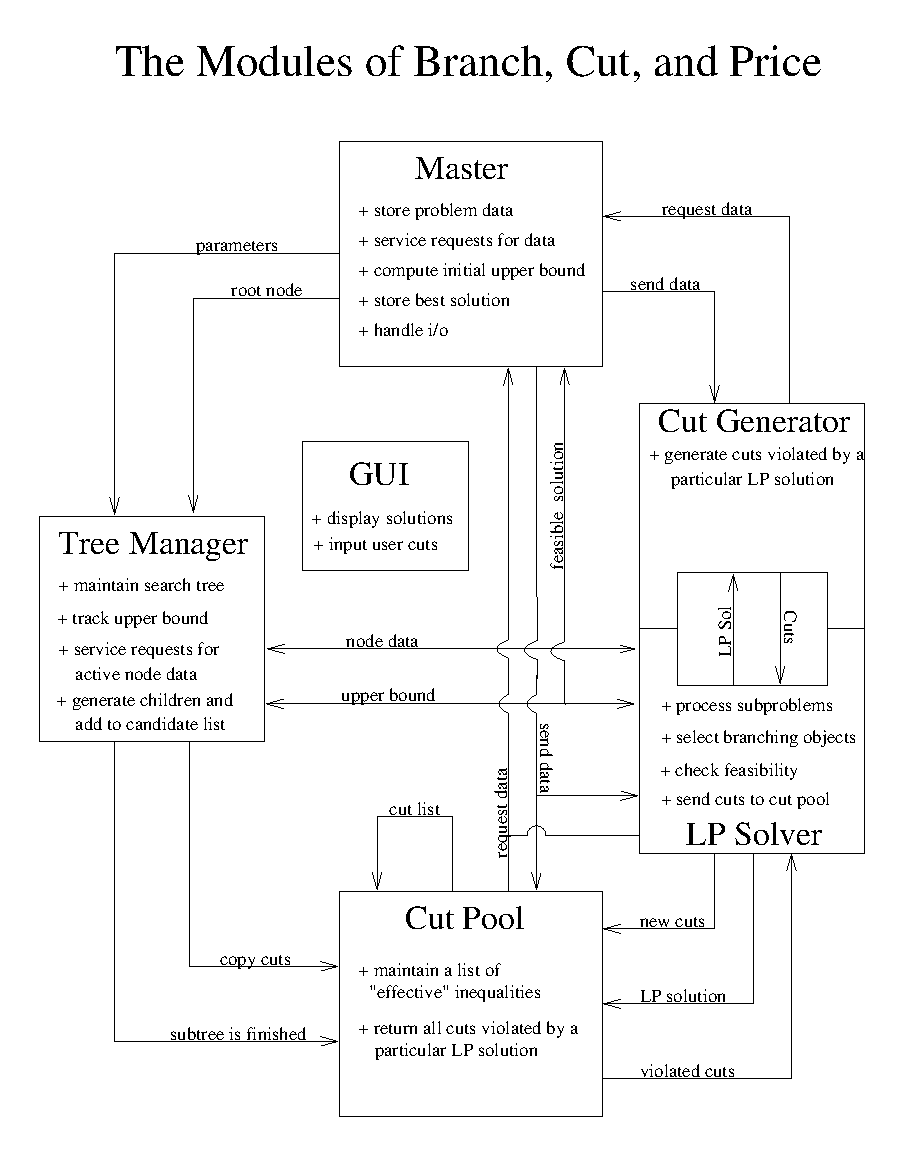
\includegraphics{pbandc}
\caption{Schematic overview of the branch, cut, and price algorithm}
\label{overview}
\end{figure}

\subsubsection{The Master Module}
\label{master-process}

The {\em master module} includes functions that perform problem initialization
and I/O. This module is the only persistent module and stores all static
problem data. The other modules are created only during a solve call and
destroyed afterward. All calls to the API are processed through the master
module. These functions of the master module implement the following tasks:
%\underbar{Overall Function:} Handle input/output, maintain the data
%for the problem instance and serve requests to send out that
%data. Keep track of the best solution found so far.\\
%\underbar{Specific Functions:}
\begin{itemize}
        \item Initialize the environment.
        \item Set and maintain parameter values.
        \item Read and store static problem data for instance to be solved.
        \item Compute an initial upper bound using heuristics.
        \item Perform problem preprocessing.
        \item Initialize the solution process, pass problem information to the
        solver modules and store the results after completion of the solve 
	call.
        \item Track the status of associated processes during parallel
        solution calls.
        \item Act as a clearing house for output during the solution process.
        \item Store warm start information between solver calls.
        \item Service requests from the user through the API for problem data,
        problem modification, and parameter modification.
\end{itemize}

\subsubsection{The Tree Management Module}

The \emph{tree manager} controls the overall execution of the algorithm. It
tracks the status of its worker modules, as well as that of the search
tree, and distributes the subproblems to be processed to the node processing
module(s). Functions performed by the tree management module are:
%\underbar{Overall Function:} Start up all the processes and keep
%track of the current state of the search tree.
%\noindent \underbar{Specific Functions:} \nobreak
\begin{itemize}
        \item Receive data for the root node and place it on the list 
        of candidates for processing.
        \item Receive data for subproblems to be held for later
        processing.
        \item Handle requests from linear programming modules to
        release a subproblem for processing.
        \item Receive branching object information, set up data structures
        for the children, and add them to the list of candidate subproblems.
        \item Keep track of the global upper bound and notify all node
        processing modules when it changes.
        \item Write current state information out to disk periodically
        to allow a restart in the event of a system crash.
        \item Keep track of run data and send it to the master
        program at termination.
\end{itemize} 

\subsubsection{The Node Processing Module}

The \emph{node processing} (NP) module is the most complex and
computationally intensive of the five processes. Its job is to perform
the bounding and branching operations. These operations
are, of course, central to the performance of the algorithm. Functions
performed by the LP module are:
%\underbar{Overall Function:} Process and bound subproblems. Branch and
%produce new subproblems. \\
%\underbar{Specific Functions:} 
\begin{itemize}
        \item Inform the tree manager when a new subproblem is needed.
        \item Receive a subproblem and process it in conjunction
        with the cut generator and the cut pool.
        \item Decide which cuts should be sent to the global pool to
        be made available to other NP modules.
        \item If necessary, choose a branching object and send its
        description back to the tree manager.
        \item Perform the fathoming operation, including generating
        variables. 
\end{itemize} 

\subsubsection{The Cut Generation Module}

The {\em cut generator} performs only one function---generating valid
inequalities violated by the current fractional solution and sending
them back to the requesting LP process. Here are the functions
performed by the cut generator module:
%\underbar{Overall Function:} Receive solution vectors from the LP
%processes and generate valid inequalities violated by these vectors.\\
%\underbar{Specific Functions:}
\begin{itemize}
        \item Receive an LP solution and attempt to
        separate it from the convex hull of all solutions.
        \item Send generated valid inequalities back to the NP module.  
        \item When finished processing a solution vector, inform the
        NP module not to expect any more cuts in case it is still waiting.
\end{itemize}

\subsubsection{The Cut Management Module}

The concept of a {\em cut pool} was first suggested by Padberg and
Rinaldi \cite{padb:branc}, and is based on the observation that in BCP, the
inequalities which are generated while processing a particular node in
the search tree are also generally valid and potentially useful at
other nodes. Since generating these cuts is usually a relatively
expensive operation, the cut pool maintains a list of the ``best'' or
``strongest'' cuts found in the tree so far for use in processing
future subproblems. Hence, the cut manager functions as an auxiliary cut
generator. More explicitly, here are the functions of the cut pool
module:
%\underbar{Overall Function:} Maintain a list of ``effective'' valid
%inequalities for use in processing the subproblems.\\
%\underbar{Specific Functions:}
\begin{itemize}
        \item Receive cuts generated by other modules and store them.
        \item Receive an LP solution and return a
set of cuts which this solution violates.
        \item Periodically purge ``ineffective'' and duplicate cuts
to control its size.
\end{itemize}

\subsection{Algorithm Summary}
\label{symphony}

Currently, \BB\ is what is known as a single-pool BCP algorithm.
The term {\em single-pool} refers to the fact that there is a single
central list of candidate subproblems to be processed, which is
maintained by the tree manager. Most sequential implementations use
such a single-pool scheme. However, other schemes may be used in
parallel implementations. For a description of various types of
parallel branch and bound, see \cite{gend:paral}.

The user begins by initializing the SYMPHONY environment and can then invoke
subroutines for reading in parameters and problem data, finding an initial
upper bound, and designating the initial set of active cuts and variables in
the root node. Once the user invokes a solve routine, a tree manager is
created to manage the solution process. The tree manager module in turn sets
up the cut pool module(s), the linear programming module(s), and the cut
generator module(s). Currently, there are three solve calls supported by the
API. The first call is the \emph{initial solve} (see Section
\ref{initial_solve}), which solves the problem from scratch without using warm
start information. The second type of solve call is a \emph{warm solve}, which
solves the problem using previously computed warm start information (see
Section \ref{warm_solve}). Finally, there is a \emph{multicriteria solve} call
which is used to enumerate efficient solutions to a given multicriteria MILP
(see Section \ref{mc_solve}).

During the solution process, the tree manager functions control the execution
by maintaining the list of candidate subproblems and sending them to the NP
modules as they become idle. The NP modules receive nodes from the tree
manager, process them, branch (if required), and send back the identity of the
chosen branching object to the tree manager, which in turn generates the
children and places them on the list of candidates to be processed (see
Section \ref{branching} for a description of the branching operation). A
schematic summary of the algorithm is shown in Figure \ref{overview}. The
preference ordering for processing nodes is a run-time parameter. Typically,
the node with the smallest lower bound is chosen to be processed next since
this strategy minimizes the overall size of the search tree. However, at
times, it is advantageous to {\em dive} down in the tree. The concepts of {\em
diving} and {\em search chains}, introduced in Section \ref{tree-management},
extend the basic ``best-first'' approach.

We mentioned earlier that cuts and variables can be treated in a
somewhat symmetric fashion. However, it should be clear by now
that our current implementation favors the implementation of
branch and cut algorithms, where the computational effort spent
generating cuts dominates that of generating variables. Our methods of
representation also clearly favor such problems. In a future version
of the software, we plan to erase this bias by adding additional
functionality for handling variable generation and storage. This is
the approach already taken by of COIN/BCP \cite{coin-or}. For more
discussion of the reasons for this bias and the differences between
the treatment of cuts and variables, see Section \ref{lp-relaxation}.

\section{Details of the Implementation}
\label{modules}

\subsection{The Master Module}
\label{master}

The primary functions performed by the master module were listed in
Section \ref{master-process}. Here, we describe the implementational details of
the various solve calls.  
%If needed, the user must provide a
%routine to read problem-specific parameters in from the parameter
%file. She must also provide a subroutine for upper bounding if
%desired, though upper bounds can also be provided explicitly. A good
%initial upper bound can dramatically decrease the solution time by
%allowing more variable-fixing and earlier pruning of search tree
%nodes. If no upper bounding subroutine is available, then the
%two-phase algorithm, in which a good upper bound is found quickly in
%the first phase using a reduced set of variables can be advantageous.
%See Section \ref{two-phase} for details. The user's only unavoidable
%obligation during pre-processing is to specify the list of base
%variables and, if desired, the list of extra variables that are to be
%active in the root node. Again, we point out that selecting a good set
%of base variables can make a marked difference in solution speed,
%especially using the two-phase algorithm.

\subsubsection{Initial Solve}\label{initial_solve}

Calling the initial solve method solves a given MILP from scratch, as
described above. The first action taken is to create an instance of the tree
manager module that will control execution of the algorithm. If the algorithm
is to be executed in parallel on a distributed architecture, the master module
spawns a separate tree manager process that will autonomously control the
solution process. The tree manager in turn creates the modules for processing
the nodes of the search tree, generating cuts, and maintaining cut pools.
These modules work in concert to execute the solution process. When it makes
sense, sets of two or more modules, such as a node processing module and a cut
generation module may be combined to yield a single process in which the
combined modules work in concert and communicate with each other through
shared memory instead of across the network. When running as separate process,
the modules communicate with each other using a standard communications
protocol. Currently, the only option supported is PVM, but it would be
relatively easy to add an MPI implementation.

The overall flow of the algorithm is similar to other branch and bound
implementations and is detailed below. A priority queue of candidate
subproblems available for processing is maintained at all times and the
candidates are processed in an order determined by the search strategy. The
algorithm terminates when the queue is empty or when another specified
condition is satisfied. A new feature in SYMPHONY \VER\  is the ability to stop
the computation based on exceeding a given time limit, exceeding a given limit
on the number of processed nodes, achieving a target percentage gap between
the upper and lower bounds, or finding the first feasible solution. After
halting prematurely, the computation can be restarted after modifying
parameters or problem data. This enables the implementation of a wide range of
dynamic and on-line solution algorithms, as we describe next.

\subsubsection{Solve from Warm Start} \label{warm_solve}

Among the utility classes in the COIN-OR repository is a base class for
describing the data needed to warm start the solution process for a particular
solver or class of solvers. To support this option for SYMPHONY, we have
implemented such a warm start class for MILPs. The main content of the class
is a compact description of the search tree at the time the computation was
halted. This description contains complete information about the subproblem
corresponding to each node in the search tree, including the branching
decisions that lead to the creation of the node, the list of active variables
and constraints, and warm start information for the subproblem itself (which
is a linear program). All information is stored compactly using SYMPHONY's
native data structures, which store only the differences between a child and
its parent, rather than an explicit description of every node. This approach
reduces the tree's description to a fraction of the size it would otherwise
be. In addition to the tree itself, other relevant information regarding the
status of the computation is recorded, such as the current bounds and best
feasible solution found so far. Using the warm start class, the user can save
a warm start to disk, read one from disk, or restart the computation at any
point after modifying parameters or the problem data itself. This allows
the user to easily implement periodic checkpointing, to design dynamic
algorithms in which the parameters are modified after the gap reaches a
certain threshold, or to modify problem data during the solution process if
needed.

\paragraph{Modifying Parameters.}

The most straightforward use of the warm start class is to restart the solver
after modifying problem parameters. To start the computation from a given warm
start when the problem data has not been modified, the tree manager simply
traverses the tree and adds those nodes marked as candidates for processing to
the node queue. Once the queue has been reformed, the algorithm is then able
to pick up exactly where it left off. Code for using the resolve command was
shown in Figure \ref{dynamic}. The situation is more challenging if the user
modifies problem data in between calls to the solver. We address this
situation next.

\paragraph{Modifying Problem Data.}

If the user modifies problem data in between calls to the solver, SYMPHONY
must make corresponding modifications to the leaf nodes of the current search
tree to allow execution of the algorithm to continue. In principle, any change
to the original data that does not invalidate the subproblem warm start data,
i.e., the basis information for the LP relaxation, can be
accommodated. Currently, SYMPHONY can only handle modifications to the rim
vectors of the original MILP. Methods for handling other modifications, such as
the addition of columns or the modification of the constraint matrix itself,
will be added in the future. To initialize the algorithm, each leaf node,
regardless of its status after termination of the previous solve call, must be
inserted into the queue of candidate nodes and reprocessed with the changed
rim vectors. After this reprocessing, the computation can continue as usual.
Optionally, the user can ``trim the tree'' before resolving. This consists of
locating nodes whose descendants are all likely to be pruned in the resolve
and eliminating those descendants in favor of processing the parent node
itself. This ability could be extended to allow changes that invalidate the
warm start data of some leaf nodes.

The ability to resolve after modifying problem data has a wide range of
applications in practice. One obvious use is to allow dynamic modification of
problem data during the solve procedure, or even after the procedure has been
completed. Implementing such a solver is simply a matter of periodically
stopping to check for user input describing a change to the problem. Another
obvious application is in situations where it is known a priori that the user
will be solving a sequence of very similar MILPs. This occurs, for instance,
when implementing algorithms for multicriteria optimization, as we describe in
Section \ref{mc_solve}. One approach to this is to solve a given ``base
problem'' (possibly limiting the size of the warm start tree), save the warm
start information from the base problem and then start each subsequent call
from this same checkpoint. Code for implementing this was shown in Figure
\ref{warm_start}. 

\subsubsection{Bicriteria Solve}\label{mc_solve}

For those readers not familiar with bicriteria integer programming, we briefly
review the basic notions here. For clarity, we restrict the discussion here to
pure integer programs (ILPs), but the principles are easily generalized. A
bicriteria ILP is a generalization of a standard ILP presented earlier that
includes a second objective function, yielding an optimization problem of the
form
\begin{equation}
\begin{array}{lrcl}
\vmin & [cx, dx],  \label{bicrit} \\
\textrm{s.t.} & Ax & \leq & b, \\ 
& x & \in & \Z^{n}.
\end{array}
\end{equation}
The operator \emph{vmin} is understood to mean that solving this program is
the problem of generating \emph{efficient} solutions, which are these feasible
solutions $p$ to \ref{bicrit} for which there does not exist a second
distinct feasible solution $q$ such that $cq \leq cp$ and $dq \leq dp$ and at
least one inequality is strict. Note that (\ref{bicrit}) does not have a
unique optimal solution value, but a set of pairs of solution values called
\emph{outcomes}. The pairs of solution values corresponding to efficient
solutions are called \emph{Pareto outcomes}. Surveys of methodology for for
enumerating the Pareto outcomes of multicriteria integer programs are provided
by Climaco et al.~\cite{climaco97} and more recently by Ehrgott and
Gandibleux~\cite{ehrgott00, ehrgott02} and Ehrgott and
Wiecek~\cite{ehrgott04}.

The bicriteria ILP (\ref{bicrit}) can be converted to a standard ILP by
taking a nonnegative linear combination of the objective
functions~\cite{geoff68}. Without loss of generality, the weights can be
scaled so they sum to one, resulting in a family of ILPs parameterized by a
scalar $0 \leq \alpha \leq 1$, with the bicriteria objective function replaced
by the \emph{weighted sum objective}
\begin{equation}\label{wsum}
(\alpha c + (1 - \alpha) d) x.
\end{equation}
Each selection of weight $\alpha$ produces a different single-objective
problem. Solving the resulting ILP produces a Pareto outcome called a
\emph{supported outcome}, since it is an extreme point on the convex lower
envelope of the set of Pareto outcomes. Unfortunately, not all efficient
outcomes are supported, so it is not possible to enumerate the set of Pareto
outcomes by solving a sequence of ILPs from this parameterized family. To
obtain all Pareto outcomes, one must replace the weighted sum objective
(\ref{wsum}) with an objective based on the \emph{weighted Chebyshev norm}
studied by Eswaran et al.~\cite{eswaran89} and Solanki~\cite{solanki91}. If
$x^c$ is a solution to a weighted sum problem with $\alpha = 1$ and $x^d$ is
the solution with $\alpha = 0$, then the weighted Chebyshev norm of a feasible
solution $p$ is
\begin{equation}
\max \{\alpha (cp - cx^c), (1 - \alpha)(dp - dx^d)\}.
\label{chebyshev}
\end{equation} 
Although this objective function is not linear, it can easily be linearized by
adding an artificial variable, resulting in a second parameterized family of
ILPs. Under the assumption of \emph{uniform dominance}, Bowman showed that an
outcome is Pareto if and only if it can be obtained by solving some ILP in
this family~\cite{bowman76}. In \cite{WCN}, the authors presented a method for
enumerating all Pareto outcomes by solving a sequence of ILPs in this
parameterized family. By slightly perturbing the objective function, they also
showed how to relax the uniform dominance assumption. Note that the set of all
supported outcomes, which can be thought of as an approximation of the set of
Pareto outcomes, can be similarly obtained by solving a sequence of ILPs with
weighted sum objectives.

SYMPHONY \VER\  contains a generic implementation of the algorithm described in
\cite{WCN}, along with a number of methods for approximating the set of Pareto
outcomes. To support these capabilities, we have extended the OSI interface so
that it allows the user to define a second objective function. Of course, we
have also added a method for invoking this bicriteria solver called
\texttt{multiCriteriaBranchAndBound()}. Relaxing the uniform dominance
requirement requires the underlying ILP solver to have the ability to
generate, among all optimal solutions to a ILP with a primary objective, a
solution minimizing a given secondary objective. We added this capability to
SYMPHONY through the use of optimality cuts, as described in \cite{WCN}.

Because implementing the algorithm requires the solution of a sequence of
ILPs that vary only in their objective functions, it is possible to use warm
starting to our advantage.  Although the linearization of (\ref{chebyshev})
requires modifying the constraint matrix from iteration to iteration, it is
easy to show that these modifications cannot invalidate the basis. In the case
of enumerating all supported outcomes, only the objective function is modified
from one iteration to the next. In both cases, we save warm start information
from the solution of the first ILP in the sequence and use it for each
subsequent computation.

\subsection{The Node Processing Module}

The NP module is at the core of the algorithm, as it performs the
processing and bounding operations for each subproblem. A schematic
diagram of the node processing loop is presented in Fig. \ref{LP-loop}.
The details of the implementation are discussed in the following
sections. 

\begin{figure}
\centering
%\psfig{figure=lploop.eps,width=4.80in}
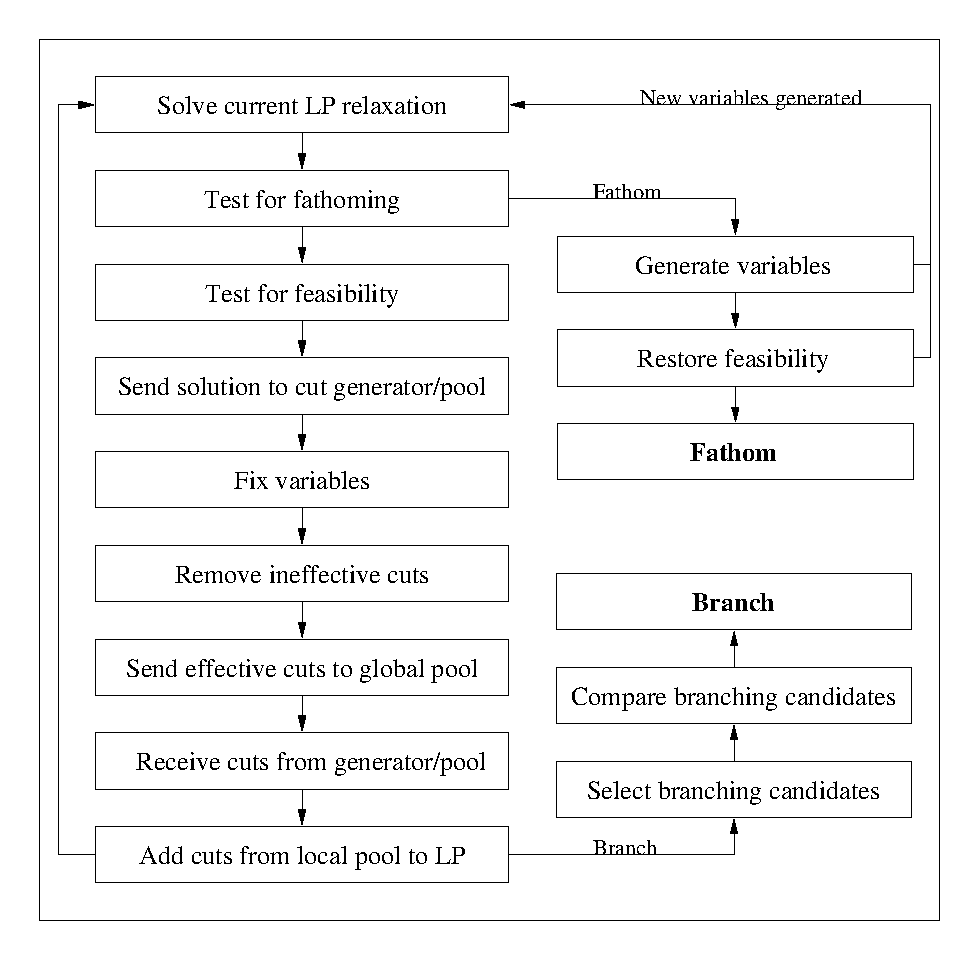
\includegraphics[width=4.8in]{lploop}
\caption{Overview of the node processing loop}
\label{LP-loop}
\end{figure}

\subsubsection{The LP Engine}

SYMPHONY requires the use of a third-party callable library (referred
to as the {\em LP engine} or {\em LP library}) to solve the LP
relaxations once they are formulated. As with the user functions,
SYMPHONY communicates with the LP engine through an API that converts
SYMPHONY's internal data structures into those of the LP engine.
Currently, the framework will only work with advanced, simplex-based
LP engines, such as CPLEX \cite{cplex}, since the LP engine must be
able to accept an advanced basis, and provide a variety of data to the
framework during the solution process. The internal data structures
used for maintaining the LP relaxations are similar to those of CPLEX
and matrices are stored in the standard column-ordered format.

\subsubsection{Managing the LP Relaxation}
\label{lp-relaxation}

The majority of the computational effort of BCP is spent
solving LPs and hence a major emphasis in the development was to make
this process as efficient as possible. Besides using a good LP engine,
the primary way in which this is done is by controlling the size of
each relaxation, both in terms of number of active variables and
number of active constraints. 

The number of constraints is controlled through use of a local
pool and through purging of ineffective constraints. When a cut is
generated by the cut generator, it is first sent to the local cut
pool. In each iteration, up to a specified number of the strongest
cuts (measured by degree of violation) from the local pool are added
to the problem. Cuts that are not strong enough to be added to the
relaxation are eventually purged from the list. In addition, cuts are
purged from the LP itself when they have been deemed ineffective for
more than a specified number of iterations, where ineffective is
defined as either (1) the corresponding slack variable is positive,
(2) the corresponding slack variable is basic, or (3) the dual value
corresponding to the row is zero (or very small). Cuts that have
remained effective in the LP for a specified number of iterations are
sent to the global pool where they can be used in later search nodes.
Cuts that have been purged from the LP can be made active again if
they later become violated.

The number of variables (columns) in the relaxation is controlled
through {\em reduced cost fixing} and {\em dynamic column generation}.
Periodically, each active variable is {\em priced} to see if it can be
fixed by reduced cost. That is, the LP reduced cost is examined in an
effort  to determine whether fixing that variable at
one of its bounds would remove improving solutions; if not, the
variable is fixed and removed from consideration. If the matrix is
{\em full} at the time of the fixing, meaning that all unfixed
variables are active, then the fixing is permanent for that subtree.
Otherwise, it is temporary and only remains in force until the next
time that columns are dynamically generated.

Because SYMPHONY was originally designed for combinatorial problems
with relatively small numbers of variables, techniques for performing
dynamic column generation are somewhat unrefined. Currently, variables
are priced out sequentially by index, which can be costly. To improve
the process of pricing variables, we plan to increase the symmetry
between our methods for handling variables and those for handling
cuts. This includes (1) allowing user-defined, abstract
representations for variables, (2) allowing the use of ``variable
generators'' analogous to cut generators, (3) implementing both global
and local pools for variables, (4) implementing heuristics that help
determine the order in which the indexed variables should be priced,
and (5) allowing for methods of simultaneously pricing out large
groups of variables. Much of this is already implemented in COIN/BCP.

Because pricing is computationally burdensome, it currently takes
place only either (1) before branching (optional), or (2) when a node
is about to be pruned (depending on the phase---see the description of
the two-phase algorithm in Sect. \ref{two-phase}). To use dynamic
column generation, the user must supply a subroutine which generates
the column corresponding to a particular user index, given the list of
active constraints in the current relaxation. When column generation
occurs, each column not currently active that has not been previously
fixed by reduced cost is either priced out immediately, or becomes
active in the current relaxation. Only a specified number of columns
may enter the problem at a time, so when that limit is reached, column
generation ceases. For further discussion of column generation, see
Sect. \ref{two-phase}, where the two-phase algorithm is described.

Since the matrix is stored in compressed form, considerable
computation may be needed to add and remove rows and columns. Hence,
rows and columns are only physically removed from the problem when
there are sufficiently many to make it ``worthwhile.'' Otherwise,
deleted rows and columns remain in the matrix but are simply ignored
by the computation. Note that because ineffective rows left in the
matrix increase the size of the basis unnecessarily, it is usually
advisable to adopt an aggressive strategy for row removal.

\subsubsection{Branching}
\label{branching}

Branching takes place whenever either (1) both cut generation and
column generation (if performed) have failed; (2) ``tailing off'' in
the objective function value has been detected; or (3) the
user chooses to force branching. Branching can take place on cuts or
variables and can be fully automated or fully controlled by the user,
as desired. Branching can result in as many children as the user
desires, though two is typical. Once it is decided that branching will
occur, the user must either select the list of candidates for {\em
strong branching} (see below for the procedure) or allow SYMPHONY to
do so automatically by using one of several built-in strategies, such
as branching on the variable whose value is farthest from being
integral. The number of candidates may depend on the level of the
current node in the tree---it is usually best to expend more effort on
branching near the top of the tree.

After the list of candidates is selected, each candidate is {\em
pre-solved}, by performing a specified number of iterations of the
dual simplex algorithm in each of the resulting subproblems. Based on
the objective function values obtained in each of the potential
children, the final branching object is selected, again either by the
user or by built-in rule. This procedure of using exploratory LP
information in this manner to select a branching candidate is commonly
referred to as {\em strong branching}. When the branching object has
been selected, the NP module sends a description of that object to the
tree manager, which then creates the children and adds them to the
list of candidate nodes. It is then up to the tree manager to specify
which node the now-idle NP module should process next. This issue is
further discussed below.

\subsection{The Tree Management Module}
\label{tree-management}

\subsubsection{Managing the Search Tree}

The tree manager's primary job is to control the execution of the
algorithm by deciding which candidate node should be chosen as the
next to be processed. This is done using either one of several
built-in rules or a user-defined rule. Usually, the goal of the search
strategy is to minimize overall running time, but it is sometimes
also important to find good feasible solutions early in the search
process. In general, there are two ways to decrease running
time---either by decreasing the size of the search tree or by
decreasing the time needed to process each search tree node.

To minimize the size of the search tree, the strategy is to select
consistently that candidate node with the smallest associated lower bound.
In theory, this strategy, sometimes called {\em best-first}, will lead
the smallest possible search tree. However, we need to consider the
time required to process each search tree node as well. This is affected
by both the quality of the current upper bound and by such factors as
communication overhead and node set-up costs. When considering these
additional factors, it is sometimes be more effective to deviate from the
best-first search order. We discuss the importance of such strategies
below.

\subsubsection{Search Chains and Diving}

One reason for not strictly enforcing the search order is because it
is somewhat expensive to construct a search node, send it to an NP
module, and set it up for processing. If, after branching, we choose
to continue processing one of the children of the current subproblem,
we avoid the set-up cost, as well as the cost of communicating the
node description of the retained child subproblem back to the tree
manager. This is called {\em diving} and the resulting chain of nodes
is called a {\em search chain}. There are a number of rules for
deciding when an NP module should be allowed to dive. One such rule is
to look at the number of variables in the current LP solution that
have fractional values. When this number is low, there may be a good
chance of finding a feasible integer solution quickly by diving. This
rule has the advantage of not requiring any global information. We
also dive if one of the children is ``close'' to being the best node,
where ``close'' is defined by a chosen parameter.

In addition to the time saved by avoiding reconstruction of the LP in
the child, diving has the advantage of often leading quickly to the
discovery of feasible solutions, as discussed above. Good upper bounds
not only allow earlier pruning of unpromising search chains, but also
should decrease the time needed to process each search tree node by
allowing variables to be fixed by reduced cost.

\subsubsection{The Two-Phase Algorithm}
\label{two-phase}

If no heuristic subroutine is available for generating feasible
solutions quickly, then a unique two-phase algorithm can also be
invoked. In the two-phase method, the algorithm is first run to
completion on a specified set of core variables. Any node that would
have been pruned in the first phase is instead sent to a pool of
candidates for the second phase. If the set of core variables is
small, but well-chosen, this first phase should be finished quickly
and should result in a near-optimal solution. In addition, the first
phase will produce a list of useful cuts. Using the upper bound and
the list of cuts from the first phase, the root node is {\em
repriced}---that is, it is reprocessed with the full set of variables
and cuts. The hope is that most or all of the variables not included
in the first phase will be priced out of the problem in the new root
node. Any variable thus priced out can be eliminated from the problem
globally. If we are successful at pricing out all of the inactive
variables, we have shown that the solution from the first phase was,
in fact, optimal. If not, we must go back and price out the (reduced)
set of extra variables in each leaf of the search tree produced during
the first phase. We then continue processing any node in which we fail
to price out all the variables.

In order to avoid pricing variables in every leaf of the tree, we can
{\em trim the tree} before the start of the second phase. Trimming the
tree consists of eliminating the children of any node for which
each child has lower bound above the current upper
bound. We then reprocess the parent node itself. This is typically
more efficient, since there is a high probability that, given the new
upper bound and cuts, we will be able to prune the parent node and
avoid the task of processing each child individually.

\subsection{The Cut Generation Module}

To implement the cut generator process, the user must provide a
function that accepts an LP solution and returns cuts violated by that
solution to the NP module. In parallel configurations, each cut is
returned immediately to the NP module, rather than being passed back
as a group once the function exits. This allows the LP to begin adding
cuts and solving the current relaxation before the cut generator is
finished if desired. Parameters controlling if and when the LP should
begin solving the relaxation before the cut generator is finished can
be set by the user.

SYMPHONY generates generic cutting planes using the Cut Generator Library,
also available from 
\htmladdnormallink{COIN-OR}{https://github.com/coin-or/Cgl}
The CGL can be used to generate cuts in cases where problem-specific cutting
planes are not available or not implemented yet. 

\subsection{The Cut Management Module}

\subsubsection{Maintaining and Scanning the Pool}

The cut manager's primary job is to receive a solution from an
NP module and return cuts from the pool that are violated by it. The
cuts are stored along with two pieces of information---the level of
the tree on which the cut was generated, known simply as the {\em
level} of the cut, and the number of times it has been checked for
violation since the last time it was actually found to be violated,
known as the number of {\em touches}. The number of touches
can be used as a simplistic measure of its effectiveness. Since the pool
can get quite large, the user can choose to scan only cuts whose
number of touches is below a specified threshold and/or cuts that were
generated on a level at or above the current one in the tree. The idea
behind this second criterion is to try to avoid checking cuts that were
not generated ``nearby'' in the tree, as they are less likely to be
effective. Any cut generated at a level in the tree
below the level of the current node must have been generated in a
different part of the tree. Although this is admittedly a naive
method, it does seem to work reasonably well.

On the other hand, the user may define a specific measure of quality for
each cut to be used instead. For example, the degree of
violation is an obvious candidate. This measure of quality must be
computed by the user, since the cut pool module has no knowledge of
the cut data structures. The quality is recomputed every time
the user checks the cut for violation and a running average is used as
the global quality measure. The cuts in the pool are periodically
sorted by this measure and only the highest quality cuts
are checked each time. All duplicate cuts, as well as all cuts whose
number of touches exceeds or whose quality falls below specified
thresholds, are periodically purged from the pool to keep it as small as
possible.

\subsubsection{Using Multiple Pools}
\label{multi-cut-pools}

For several reasons, it may be desirable to have multiple cut pools.
When there are multiple cut pools, each pool is initially assigned
to a particular node in the search tree. After being assigned to that
node, the pool services requests for cuts from that node and all
of its descendants until such time as one of its descendants gets
assigned to another cut pool. After that, it continues to
serve all the descendants of its assigned node that are not assigned
to other cut pools.

Initially, the first cut pool is assigned to the root node. All other cut
pools are unassigned. During execution, when a new node is sent to be
processed, the tree manager must determine which cut pool the node should be
serviced by. The default is to use the same cut pool as its parent. However,
if there is currently an idle cut pool process (either it has never been
assigned to any node or all the descendants of its assigned node have been
processed or reassigned), then that cut pool is assigned to this new node. All
the cuts currently in the cut pool of its parent node are copied to the new
pool to initialize it, after which the two pools operate independently on
their respective subtrees. When generating cuts, the NP module sends the new
cuts to the cut pool assigned to service the node during whose processing the
cuts were generated.

The primary motivation behind the idea of multiple cut pools is
two-fold. First, we want simply to limit the size of each pool as
much as possible. By limiting the number of nodes that a cut pool has
to service, the number of cuts in the pool will be similarly limited.
This not only allows cut storage to spread over multiple processors,
and hence increases the available memory, but at the same time, the
efficiency with which the cut pool can be scanned for violated cuts is
also increased. A secondary reason for maintaining multiple cut pools is
that it allows us to limit the scanning of cuts to only those that
were generated in the same subtree as the current search node. As
described above, this helps focus the search and should increase the
efficiency and effectiveness of the search. This idea also
allows us to generate locally valid cuts, such as the classical
Gomory cuts (see \cite{nemwol88}).

\section{Parallelizing BCP}
\label{parallelizing}

Because of the clear partitioning of work that occurs when the
branching operation generates new subproblems, branch and bound
algorithms lend themselves well to parallelization. As a result, there
is already a significant body of research on performing branch and
bound in parallel environments. We again point the reader to the
survey of parallel branch and bound algorithms by Gendron and Crainic
\cite{gend:paral}, as well as other references such as
\cite{PICO,GraKum99,kuma:para4,kuma:para3}.

In parallel BCP, as in general branch and bound, there are two major
sources of parallelism. First, it is clear that any number of
subproblems on the current candidate list can be processed
simultaneously. Once a subproblem has been added to the list, it can
be properly processed before, during, or after the processing of any
other subproblem. This is not to say that processing a particular node
at a different point in the algorithm won't produce different
results---it most certainly will---but the algorithm will terminate
correctly in any case. The second major source of parallelism is to
parallelize the processing of individual subproblems. By allowing
separation to be performed in parallel with the solution of the linear
programs, we can theoretically process a node in little more than the
amount of time it takes to solve the sequence of LP relaxations. Both
of these sources of parallelism can be easily exploited using the
\BB\ framework.

The most straightforward parallel implementation, which is the one we
currently employ, is a master-slave model, in which there is a central
manager responsible for partitioning the work and parceling it out to
the various slave processes that perform the actual computation. The
reason we chose this approach is because it allows memory-efficient
data structures for sequential computation and yet is conceptually
easy to parallelize. Unfortunately, this approach does have limited
scalability. For further discussions on the scalability of BCP algorithms and
approaches to improving it, see \cite{symphony1} and \cite{ALPS2}.

%\subsection{Details of the Parallel Implementation}

\subsection{Parallel Configurations}

SYMPHONY supports numerous configurations, ranging from completely
sequential to fully parallel, allowing efficient execution in many
different computational settings. As described in the previous
section, there are five modules in the standard distributed
configuration. Various subsets of these modules can be
combined to form separate executables capable of communicating
with each other across a network. When two or more modules are combined,
they simply communicate through shared-memory instead of through
message-passing. However, they are also forced to run in sequential
fashion in this case, unless the user chooses to enable threading
using an OpenMP compliant compiler (see next section). 

As an example, the default distributed configuration includes a
separate executable for each module type, allowing full parallelism.
However, if cut generation is fast and not memory-intensive,
it may not be worthwhile to have the NP module and its associated cut
generator work independently, as this increases communication
overhead without much potential benefit. In this case, the cut
generator functions can be called directly from the NP module,
creating a single, more efficient executable.

\subsection{Inter-process Communication}

SYMPHONY can utilize any third-party communication protocol supporting basic
message-passing functions. All communication subroutines interface with
SYMPHONY through a separate communications API. Currently, PVM \cite{PVMbook}
is the only message-passing protocol supported, but interfacing with another
protocol is a straightforward exercise.

Additionally, it is possible to configure the code to run in parallel using
threading to process multiple search tree nodes simultaneously. Currently,
this is implemented using OpenMP compiler directives to specify the parallel
regions of the code and perform memory locking functions. Compiling the code
with an OpenMP compliant compiler will result in a shared-memory parallel
executable. For a list of OpenMP compliant compilers and other resources,
visit \code{\url{http://www.openmp.org}}.

\subsection{Fault Tolerance}
\label{fault-tolerance} 

Fault tolerance is an important consideration for solving large problems on
computing networks whose nodes may fail unpredictably. The tree manager tracks
the status of all processes and can restart them as necessary. Since the state
of the entire tree is known at all times, the most that will be lost if an NP
module or cut generator is killed is the work that had been completed on that
particular search node. To protect against the tree manager itself or a cut
pool being killed, full logging capabilities have been implemented. If
desired, the tree manager can write out the entire state of the tree to disk
periodically, allowing a warm restart if a fault occurs. Similarly, the cut
pool process can be warm-started from a log file. This not only allows for
fault tolerance but also for full reconfiguration in the middle of solving a
long-running problem. Such reconfiguration could consist of anything from
adding more processors to moving the entire solution process to another
network.



\chapter{Developing Custom Applications}
\label{SYMPHONY-development}
%===========================================================================%
%                                                                           %
% This file is part of the documentation for the SYMPHONY MILP Solver.      %
%                                                                           %
% SYMPHONY was jointly developed by Ted Ralphs (ted@lehigh.edu) and         %
% Laci Ladanyi (ladanyi@us.ibm.com).                                        %
%                                                                           %
% (c) Copyright 2000-2015 Ted Ralphs. All Rights Reserved.                  %
%                                                                           %
% SYMPHONY is licensed under the Eclipse Public License. Please see         %
% accompanying file for terms.                                              %
%                                                                           %
%===========================================================================%

\section{Navigating the Source Code}

To develop an application with SYMPHONY, you need to first understand how the
source files are organized. Note that in this chapter, all path names are
given Unix-style. When you unpack the \BB\ source distribution, you will
notice at the root level a number of files associated with the automatic
configuration system, as well as a number of subdirectories, each of which
corresponds to a library used by SYMPHONY for some specific functionality. The
files associated with SYMPHONY itself are located in the \code{SYMPHONY}
subdirectory. Within the SYMPHONY subdirectory are a number of other
subdirectories, including one called \code{src} containing the source files
for SYMPHONY itself. 

Also in the main \code{SYMPHONY/} subdirectory, there is a subdirectory called
\code{Applications/} (see Sections~\ref{build_appl_unix} and
\ref{build_appl_msvc}) for instructions on building the applications). The
\code{Applications/} subdirectory contains the source code for a number of
sample applications developed with SYMPHONY, as well as function stubs for
developing a custom application using SYMPHONY's callbacks. The subdirectory
\code{SYMPHONY/Applications/USER} contains the files needed for implementing
the callbacks and is a template for developing an application. In this
directory and its subdirectories, which mirror the subdirectories of SYMPHONY
itself, each file contains function stubs that can be filled in to create a
new custom application. There is a separate subdirectory for each
module---master (\code{Master/}), tree management (\code{TreeManager/}), cut
generation (\code{CutGen/}), cut management (\code{CutPool/}), and node
processing (\code{LP/}). Within each subdirectory, there is a file, initially
called \code{USER/*/user\_*.c}, where \code{*} is the name of the module. The
primary thing that you, as the user, need to understand to build a custom
application is how to fill in these stubs. That is what the second part of
this chapter is about. Before describing that, however, we will discuss how to
build your application. 

%Within the \code{src} subdirectory, the files are
%organized along the lines of the modules. There is a separate subdirectory for
%each module---master (\code{Master/}), tree management (\code{TreeManager/}),
%cut generation (\code{CutGen/}), cut management (\code{CutPool/}), and node
%processing (\code{LP/}). In addition, there are directories called
%\code{DrawGraph/} and \code{Common/} that also contain source files. The
%\code{DrawGraph/} directory provides an interface from \BB\ to the
%\emph{Interactive Graph Drawing} software package developed by Marta Es\"o.
%This is an excellent utility for graphical display and debugging. The
%\code{Common/} directory contains source code for functions used by multiple
%modules.

%Within each module's directory, there is a primary source file containing the
%function \code{main()} (named \code{*.c} where \code{*} is the module name), a
%source file containing functions related to inter-process communication (named
%\code{*\_proccomm.c}) and a file containing general subroutines used by the
%module (named \code{*\_func.c}). The master is the exception and is organized
%slightly differently. The LP process source code is further subdivided due to
%the sheer number of functions.

%In the main \code{SYMPHONY/} subdirectory (at the same level as the
%\code{src/} subdirectory), there is also a subdirectory called \code{include/}
%that contains the header files. Corresponding to each module, there are three
%header files, one containing internal data structures and function prototypes
%associated with the module (named \code{sym\_*.h} where * is the module name),
%one containing the data structures for storing the parameters (these are also
%used by the master process), and the third containing the function prototypes
%for the user callbacks (name \code{sym\_*\_u.h}). By looking at the header
%files, you should get a general idea of how things are laid out.

%FIXME: Check this
\section{Building an Application}
\label{building_custom_app}

Note that the template application can be built and will work without
modifying any of the source files. In this case, SYMPHONY will behave
according to default settings. 

\subsection{Unix}

First, download and build SYMPHONY as described in Section
\ref{build_appl_unix}. This will generate the required library and makefiles
for each application. After this, typing \code{make} in the
\code{SYMPHONY/Applications/USER/} subdirectory should successfully build the
executable. For more information, including the parallel configuration
instructions, see the \code{SYMPHONY/Applications/USER/INSTALL} file.

\subsection{Microsoft Visual C++}

First, download \code{SYMPHONY-\VER} and unpack the archive if it is
required. You now have three options. You can either compile on the
command-line using the automated DEVENV build system or NMAKE utility or you
can use the provided project and solution files. For all of the following
options, first go to the \code{SYMPHONY\bs Applications\bs USER\bs
MSVisualStudio \bs v8} directory.

\subsubsection{Using the MSDEV Utility}
\begin{itemize}
\item Open a command line terminal and type
{\color{brown}
\begin{verbatim}
 devenv user.sln /Build "Win32|Release"
\end{verbatim}
} 
This will create both the release version of the USER application, including
the executable \code{user} and the SYMPHONY library needed for linking with
applications.

\item To test the executable, type 
{\color{brown}
\begin{verbatim}
 Debug\user.exe -F ..\..\sample.user
\end{verbatim}
}
\item If USER source files are modified, type 
{\color{brown}
\begin{verbatim}
 devenv user.sln /make all /rebuild
\end{verbatim}
}
in order to clean and rebuild everything.
\end{itemize} 

\subsubsection{Using the MSVC++ IDE}

\begin{itemize}
\item Open the solution file \code{user.sln}.

\item 
The configuration steps are exactly the same with the MSVC++ section of 
\code{SYMPHONY}. The only 
difference is that, you have the \code{user} project instead of the
\code{symphony} project. Go through the related steps of section 
\ref{getting_started_windows} to see how to get USER executable. 

\item
Once you have the proper settings, choose \code{Build
user.exe} from the \code{Build} menu. This should successfully 
build the executable.

\item
To test the executable, right click on the \code{user} project, go to the
\code{Debug} tab and set the program arguments to 
\code{-F ..\bs ..\bs sample.mps}. Note that command-line switches are 
Unix-style.

\item
Now choose \code{Execute} from the build menu and you have a working branch
and bound solver! After successful compilation, you can fill in the user
callback functions as describe in Section \ref{SYMPHONY-development}.
\end{itemize}

\section{Writing the Callbacks}

For each module, all callback functions are invoked from so-called
\emph{wrapper functions} that provide the interface and also performs a
default action if the user chooses not to override it. Although SYMPHONY is
written in C, the wrapper functions provide a C++-style interface in which the
user can either accept the default action or override it. Each wrapper
function is named \code{*\_u()} , where \code{*} is the name of the
corresponding callback function, and is defined in a file called
\code{*\_wrapper.c}. The wrapper function first collects the necessary data
and hands it to the user by calling the user function. Based on the return
value from the user, the wrapper then performs any necessary post-processing.
All callback functions have default options, so that SYMPHONY now acts as a
generic MILP solver out of the box.

In Section \ref{API}, the callback functions are described in
detail.  The name of every callback function starts with \code{user\_}.
There are three kinds of arguments:
\begin{description}
\item[\rm IN:] An argument containing information that the user might need
to perform the function.
\item[\rm OUT:] A pointer to an argument in which the user should
return a result (requested data, decision, etc.) of the function. 
\item[\rm INOUT:] An argument which contains information the user might need,
but also for which the user can change the value.
\end{description}
The return values for most function are as follows:
\begin{description}
\item[Return values:] \hfill

\begin{tabular}{lp{310pt}} 

\code{USER\_ERROR} & Error in the user function. Printing an error message is
the user's responsibility. Depending on the work the user function was
supposed to do, the error might be ignored (and some default option used), or
the process aborts. \\

\code{USER\_SUCCESS} & The user function was implemented and executed correctly. \\

\code{USER\_DEFAULT} & This option means that the user function was not
implemented and that SYMPHONY should either execute a default subroutine (the
default is one of the built-in options---\BB\ decides which one to use based on
initial parameter settings and the execution of the algorithm) or else do
nothing, if execution of the subroutine is optional. \\

\code{built\_in\_option1 } & \\
\code{built\_in\_option2 } ... & The specified built-in option will be used.\\
\end{tabular}

\item[Notes:] \hfill
\begin{itemize}
\vspace{-3ex}

\item Sometimes an output is optional. This is always noted in the
function descriptions.

\item If an array has to be returned (i.e., the argument is \code{type
  **array}), then (unless otherwise noted) the user has to allocate space for
  the array itself and set \code{*array} to be the array allocated. If an
  output array is optional and the user is not returning any values in that
  array, then the user {\em must not} set \code{*array} because this is how
  \BB\ decides which optional arrays are filled up.

\item Some built-in options are implemented so that the user can invoke them
directly from the callback function. This might be useful if, for example,
the user wants to use different built-in options at different stages
of the algorithm.
\end{itemize}

\end{description}

\section{Data Structures}

The user can define her own data structure for each module to maintain problem
data and any other information the user needs access to in order to implement
functions to customize the solver. A pointer to this data structure is
maintained by \BB\ and is passed to the user as an argument to each user
function. The pointer must be initially passed using the
\ptt{sym\_set\_user\_data()} command. Since \BB\ knows nothing about this data
structure, it is up to the user to allocate it and maintain it. The user must
also implement a function to free it. The functions for freeing the user data
structures in each module are called \code{user\_free\_*}, where \code{*} is
the module. These functions are called by SYMPHONY at the time when other data
structures for the modules are being freed and the module is being closed. By
default, for sequential computation, there is one common user data structure
for all modules and the pointer to that data structure is passed to all user
functions, regardless of the module. This setup should work fine for most
sequential applications. In parallel, however, pointers cannot be shared
between modules and data must be explicitly passed. In this case, it is
sometimes more efficient to maintain in each module only the data necessary to
perform the functions of that module.

\section{Parallel Implementation}

\subsection{Distributed-memory Architectures}
\label{communication}

While the implementation of \BB\ strives to shield the user from having to
know anything about communications protocols or the specifics of inter-process
communication, it may be necessary for the user to pass information from one
module to another in order to implement a parallel application. For instance,
the user may want to pass data describing the problem instance to the LP
process after reading them in from a file in the master process. For the
purpose of passing user data from the master process to other processes, a
customization function called
\code{user\_send\_*\_data()} is provided in the master module, along with a
corresponding function called \code{user\_receive\_*\_data()} in the module
\code{*}. These two functions work in tandem to transport the user's data
from the maser, where it can be read in from a file, to the proper module for
processing. There are also a number of other tandem pairs of \emph{send} and
\emph{receive} functions that are used to transport user data from place to
place.

All data are sent in the form of arrays of either type \code{char}, \code{int},
or \code{double}, or as strings. To send an array, the user has simply to
invoke the function \code{send\_XXX\_array(XXX *array, int length)} where
\code{XXX} is one of the previously listed types. To receive that array,
there is a corresponding function called \code{receive\_?\_array(?  *array, int
length)}. When receiving an array, the user must first allocate the
appropriate amount of memory. In cases where variable length arrays need to be
passed, the user must first pass the length of the array (as a separate array
of length one) and then the array itself. In the receive function, this allows
the length to be received first so that the proper amount of space can be
allocated before receiving the array itself. Note that data must be received
in exactly the same order as it was passed, as data is read linearly into and
out of the message buffer. The easiest way to ensure this is done properly is
to simply copy the send statements into the receive function and change the
function names. It may then be necessary to add some allocation statements in
between the receive function calls.

\subsection{Shared-memory Architectures}
\label{shared}

In the shared memory configuration, it is not necessary to use
message passing to move information from one module to another since
memory is globally accessible. In the few cases where the user would
ordinarily have to pass information using message passing, it is
easiest and most efficient to simply copy the information to the new
location. This copying gets done in the {\em send} function and hence
the {\em receive} function is never actually called. This means that
the user must perform all necessary initialization, etc. in the send
function. This makes it a little confusing to write source code which
will work for all configurations. However, the confusion should be
minimized by looking at the sample applications, especially the VRP solver,
which works in all configurations, sequential, distributed parallel, and
shared parallel. 

%\subsection{Unix Operating Systems}

%Once the callback functions are filled in, all that remains is to compile the
%application. The distribution comes with two makefiles that facilitate this
%process. The primary makefile resides in the {\tt SYMPHONY-\VER/} directory.
%The user makefile resides in the user's subdirectory, initially called
%\code{SYMPHONY-\VER/SYMPHONY/Applications/USER/}. This subdirectory can be
%moved, as well as renamed. There are a number of variables that must be set in
%the primary make file. To modify the makefiles appropriately, see the
%instructions in Section \ref{getting_started_unix}.

%\subsection{Microsoft Windows}

%First, follow the instructions for compiling SYMPHONY in Section
%\ref{getting_started_windows} to ensure you have the proper settings. Once the
%stub files in the {\tt SYMPHONY-\VER\bs SYMPHONY\bs Applications \bs USER}
%hierarchy are filled in, you should be able to compile the new application and
%run it successfully.

\section{Debugging Your Application}

Much of this section applies to Unix operating systems. However, it may
also be useful for Windows users.

\subsection{The First Rule}

\BB\ has many built-in options to make debugging easier. The most
important one, however, is the following rule. {\bf It is easier to
debug the fully sequential version than the fully distributed
version}. Debugging parallel code is not terrible, but it is more
difficult to understand what is going on when you have to look at the
interaction of several different modules running as separate
processes. This means multiple debugging windows which have to be
closed and restarted each time the application is re-run. For this
reason, it is highly recommended to develop code that can be compiled
serially even if you eventually intend to run in a fully distributed
environment. This does make the coding marginally more complex, but
believe me, it's worth the effort. The vast majority of your code will
be the same for either case. Make sure to use the configuration flag to
\code{--enable-debug} while building (see Section \ref{building_from_source}). 

\subsection{Debugging with PVM}
\label{debugging-PVM}
If you wish to venture into debugging your distributed application, then you
simply need to set the parameter \code{*\_debug}, where * is the name of the
module you wish to debug, to ``1'' in the parameter file. This will tell PVM
to spawn the particular process or processes in question under a debugger.
What PVM actually does in this case is to launch the script
\code{\$PVM\_ROOT/lib/debugger}. You will undoubtedly want to modify this
script to launch your preferred debugger in the manner you deem fit. If you
have trouble with this, please send e-mail to the list serve (see Section
\ref{resources}).

It's a little tricky to debug interacting parallel processes. The main
difficulty is in that the order of operations is difficult to control. Random
interactions can occur when processes run in parallel due to varying system
loads, process priorities, etc. Therefore, it may not always be possible to
duplicate errors. To force runs that you should be able to reproduce, make
sure the parameter \ptt{no\_cut\_timeout} appears in the parameter file or
start \BB\ with the \code{-a} option. This will keep the cut generator from
timing out, a major source of randomness. Furthermore, run with only one
active node allowed at a time (set \ptt{ max\_active\_nodes} to ``1''). This
will keep the tree search from becoming random. These two steps should allow
runs to be reproduced. You still have to be careful, but this should make
things easier.

%\subsection{Using \code{Purify} and \code{Quantify}}

%The makefile is already set up for compiling applications using {\tt
%purify} and {\tt quantify}. Simply set the paths to the executables
%and type ``{\tt make pall}'' or ``{\tt p*}'' where * is the module you
%want to purify. The executable name is the same as described in
%Section \ref{distributed-build}, but with a ``p'' in front of it. To tell PVM
%to launch the purified version of the executables, you must set the
%parameters {\tt *\_exe} in the parameter file to the purified
%executable names. See Section \ref{tm_params} for information on
%setting parameters in the parameter file.

\subsection{Checking the Validity of Cuts and Tracing the Optimal Path}
\label{debugging}

Sometimes the only evidence of a bug is the fact that the optimal solution to
a particular problem is never found. This is usually caused by either (1)
adding an invalid cut, or (2) performing an invalid branching. There are two
options available for discovering such errors. The first is for checking the
validity of added cuts. This checking must, of course, be done by the user,
but \BB\ can facilitate such checking. To do this, the user must fill in the
function \hyperref{{\tt user\_check\_validity\_of\_cut()}} {\ptt{
user\_check\_validity\_of\_cut()} (see Section
}{)}{user_check_validity_of_cut}. THIS function is called every time a cut is
passed from the cut generator to the LP and can function as an independent
verifier. To do this, the user must pass (through her own data structures) a
known feasible solution. Then for each cut passed into the function, the user
can check whether the cut is satisfied by the feasible solution. If not, then
there is a problem! Of course, the problem could also be with the checking
routine. To enable this functionality, the user must configure SYMPHONY with
the flag \code{--enable-cut-check} (see Section \ref{building_from_source}). 

Tracing the optimal path can alert the user when the subproblem which admits a
particular known feasible solution (at least according to the branching
restrictions that have been imposed so far) is pruned. This could be due to an
invalid branching. Note that this option currently only works for branching on
binary variables. To use this facility, the user must fill in the function
\hyperref{{\tt user\_send\_feas\_sol()}} {\ptt {user\_send\_feas\_sol()} (see
Section }{)}{user_send_feas_sol}. All that is required is to pass out an array
of user indices that are in the feasible solution that you want to trace. Each
time the subproblem which admits this feasible solution is branched on, the
branch that continues to admit the solution is marked. When one of these
marked subproblems is pruned, the user is notified. To enable this
functionality, the user must configure SYMPHONY with the flag
\code{--enable-trace-path} (see Section \ref{building_from_source}). 


\subsection{Using the Interactive Graph Drawing Software}
\label{IGD}
The Interactive Graph Drawing (IGD) software package is included with
\BB\ and \BB\ facilitates its use through interfaces with the
package. The package, which is a Tcl/Tk application, is extremely
useful for developing and debugging applications involving graph-based
problems. Given display coordinates for each node in the graph, IGD
can display support graphs corresponding to fractional solutions with or
without edge weights and node labels and weights, as well as other
information. Furthermore, the user can interactively modify the graph
by, for instance, moving the nodes apart to ``disentangle'' the
edges. The user can also interactively enter violated cuts through the
IGD interface.

To use IGD, you must have installed PVM since the drawing window runs
as a separate application and communicates with the user's routines
through message passing. To compile the graph drawing application,
type \code{make dg} in the \BB\ root directory. The user
routines in the file \code{user\_dg.c} can be filled in, but it is not
necessary to fill anything in for basic applications. 

After compiling \code{dg}, the user must write some subroutines that
communicate with \code{dg} and cause the graph to be drawn.
Regrettably, this is currently a little more complicated than it needs
to be and is not well documented. However, by looking at the sample
application, it should be possible to see how it is done. To
enable graph drawing, put the line {\ptt {do\_draw\_graph 1} into the
parameter file or use the \code{-d} command line option. It can be difficult to
get IGD to work. If you are interested in using it and cannot get it to work,
feel free to contact me.

\subsection{Other Debugging Techniques}

Another useful built-in function is \code{write\_mps()}, which will write the
current LP relaxation to a file in MPS format. This file can then be read into
the LP solver interactively or examined by hand for errors.  Many times, CPLEX
gives much more explicit error messages interactively than through the
callable library. The form of the function is
{\color{brown}
\begin{verbatim}
void write_mps(LPdata *lp_data, char *fname)
\end{verbatim}
} where \code{fname} is the name of the file to be written. If \BB\ is forced
to abandon solution of an LP because the LP solver returns an error code, the
current LP relaxation is automatically written to the file
\code{matrix.[bc\_index].[iter\_num].mps} where \code{bc\_index} is the index
of the current subproblem and \code{iter\_num} is the current iteration
number. The \code{write\_mps()} function can be called using breakpoint code
to examine the status of the matrix at any point during execution.

Logging is another useful feature. Logging the state of the search tree can
help isolate some problems more easily. See Section \ref{tm_params}
for the appropriate parameter settings to use logging.

\section{Case Study: Implementing a Matching Solver}

This section was contributed by Michael Trick a few years ago and is a
walkthrough of the steps for developing a very simple application using
SYMPHONY. Rather than presenting the code in its final version, we will go
through the steps that a user would go through. Note that some of the code is
lifted from the vehicle routing application. This code is designed to be a
sequential code. The MATCH application discussed here is part of the SYMPHONY
distribution and the source code can be found in the
\code{SYMPHONY/Applications/MATCH} directory.

The goal is to create a minimum matching on a complete graph. Initially, we
will just formulate this as an integer program with one variable for each
possible pair that can be matched. Then we will include a set of constraints
that can be added by cut generation.

We begin with the template code in the \code{USER} subdirectory included with
SYMPHONY. This gives stubs for each user callback routine. First, I need to
define a data structure for describing an instance of the matching problem. We
use the template structure \code{USER\_PROBLEM} in the file
\code{include/user.h} for this purpose.  To describe an instance, we just
need the number of nodes and the cost matrix. In addition, we also need a way
of assigning an index to each possible assignment. Here is the data
structure: 
{\color{brown}
\begin{verbatim}
typedef struct USER_PROBLEM{
   int              numnodes;
   int              cost[MAXNODES][MAXNODES];
   int              match1[MAXNODES*(MAXNODES-1)/2];
   int              match2[MAXNODES*(MAXNODES-1)/2]; 
   int              index[MAXNODES][MAXNODES];
}user_problem;
\end{verbatim}
}
The fields \code{match1}, \code{match2}, and
\code{index} will be used later in the code in order to map variables to the
corresponding assignment and vice versa. 

Next, we need to read in the problem instance. We could implement this
function within the \code{user\_io()} callback function (see the file
\code{user\_master.c}). However, in order to show how it can be done
explicitly, we will define our own function \code{match\_read\_data()} in
\code{user\_main.c} to fill in the user data structure and then use
\code{sym\_set\_user\_data()} to pass this structure to SYMPHONY. The
template code already provides basic command-line options for the user. The
``-F'' flag is used to specify the location of a data file, from which we will
read in the data. The datafile contains first the number of nodes in the graph
(\code{nnodes}) followed by the pairwise cost matrix (nnode by nnode). We
read the file in with the \code{match\_read\_data()} routine in
\code{user\_main.c}:

%FIXME: Here, we don't need to pass in the user data structure...just return
%it. We also don't need to pass in the sym_enviroment 

{\color{brown}
\begin{verbatim}
int match_read_data(user_problem *prob, char *infile)
{
   int i, j;
   FILE *f = NULL;

   if ((f = fopen(infile, "r")) == NULL){
      printf("main(): user file %s can't be opened\n", infile);
      return(ERROR__USER); 
   }

   /* Read in the costs */
   fscanf(f,"%d",&(prob->numnodes));
   for (i = 0; i < prob->numnodes; i++)
      for (j = 0; j < prob->numnodes; j++)
         fscanf(f, "%d", &(prob->cost[i][j]));
   
   return (FUNCTION_TERMINATED_NORMALLY);
}
\end{verbatim}
}   

We can now construct the integer program itself. This is done by specifying
the constraint matrix and the rim vectors in sparse format. We will have a
variable for each possible assignment $(i,j)$ with $i<j$. We have a constraint
for each node $i$, so it can only me matched to one other node.

We define the IP in our other helper function \code{match\_load\_problem()}
in \code{user\_main.c}. In the first part of this routine, we will build a
description of the IP, and then in the second part, we will load this
representation to SYMPHONY through
\code{sym\_explicit\_load\_problem()}. Note that we could instead create a
description of each subproblem dynamically using the
\code{user\_create\_subproblem()} callback (see \code{user\_lp.c}), but
this is more complicated and unnecessary here.

{\color{brown}
\begin{verbatim}
int match_load_problem(sym_environment *env, user_problem *prob){
   
   int i, j, index, n, m, nz, *matbeg, *matind;
   double *matval, *lb, *ub, *obj, *rhs, *rngval;
   char *sense, *is_int;
   
   /* set up the inital LP data */
   n = prob->numnodes*(prob->numnodes-1)/2;
   m = 2 * prob->numnodes;
   nz = 2 * n;

   /* Allocate the arrays */
   matbeg  = (int *) malloc((n + 1) * ISIZE);
   matind  = (int *) malloc((nz) * ISIZE);
   matval  = (double *) malloc((nz) * DSIZE);
   obj     = (double *) malloc(n * DSIZE);
   lb      = (double *) calloc(n, DSIZE);
   ub      = (double *) malloc(n * DSIZE);
   rhs     = (double *) malloc(m * DSIZE);
   sense   = (char *) malloc(m * CSIZE);
   rngval  = (double *) calloc(m, DSIZE);
   is_int  = (char *) malloc(n * CSIZE);
   
   /* Fill out the appropriate data structures -- each column has
      exactly two entries */
   index = 0;
   for (i = 0; i < prob->numnodes; i++) {
      for (j = i+1; j < prob->numnodes; j++) {
         prob->match1[index] = i; /*The first component of assignment 'index'*/
         prob->match2[index] = j; /*The second component of assignment 'index'*/
         /* So we can recover the index later */
         prob->index[i][j] = prob->index[j][i] = index;
         obj[index] = prob->cost[i][j]; /* Cost of assignment (i, j) */
         is_int[index] = TRUE;
         matbeg[index] = 2*index;
         matval[2*index] = 1;
         matval[2*index+1] = 1;
         matind[2*index] = i;
         matind[2*index+1] = j;
         ub[index] = 1.0;
         index++;
      }
   }
   matbeg[n] = 2 * n;
   
   /* set the initial right hand side */
   for (i = 0; i < m; i++) {
      rhs[i] = 1;
      sense[i] = 'E';
   }
   
   /* Load the problem to SYMPHONY */   
   sym_explicit_load_problem(env, n, m, matbeg, matind, matval, lb, ub, 
                             is_int, obj, 0, sense, rhs, rngval, true);
			     
   return (FUNCTION_TERMINATED_NORMALLY);

}
\end{verbatim}
}

Now, we are ready to gather everything in the \code{main()} routine in 
\code{user\_main()}. This will involve to create a SYMPHONY environment and 
a user data structure, read in the data, create the corresponding IP, 
load it to the environment and ask SYMPHONY to solve it 
(\code{CALL\_FUNCTION} is just a macro to take care of the return values):  

{\color{brown}
\begin{verbatim}
int main(int argc, char **argv)
{
   int termcode;
   char * infile;

   /* Create a SYMPHONY environment */
   sym_environment *env = sym_open_environment();

   /* Create the data structure for storing the problem instance.*/
   user_problem *prob = (user_problem *)calloc(1, sizeof(user_problem));
   
   CALL_FUNCTION( sym_set_user_data(env, (void *)prob) );
   CALL_FUNCTION( sym_parse_command_line(env, argc, argv) );
   CALL_FUNCTION( sym_get_str_param(env, "infile_name", &infile));
   CALL_FUNCTION( match_read_data(prob, infile) );
   CALL_FUNCTION( match_load_problem(env, prob) );
   CALL_FUNCTION( sym_solve(env) );
   CALL_FUNCTION( sym_close_environment(env) );
   return(0);
}
\end{verbatim}
}

OK, that's it. That defines an integer program, and if you compile and
optimize it, the rest of the system will come together to solve this problem.
Here is a data file to use:
{\color{brown}
\begin{verbatim}
6
0 1 1 3 3 3
1 0 1 3 3 3
1 1 0 3 3 3
3 3 3 0 1 1
3 3 3 1 0 1
3 3 3 1 1 0
\end{verbatim}
}

The optimal value is 5. To display the solution, we need to be able to map
back from variables to the nodes. That was the use of the \code{node1} and
\code{node2} parts of the \code{USER\_PROBLEM}. We can now use
\code{user\_display\_solution()} in \code{user\_master.c} to print 
out the solution:

{\color{brown}
\begin{verbatim}
int user_display_solution(void *user, double lpetol, int varnum, int *indices,
                          double *values, double objval)
{
   /* This gives you access to the user data structure. */
   user_problem *prob = (user_problem *) user;
   int index;
 
   for (index = 0; index < varnum; index++){
      if (values[index] > lpetol) {
          printf("%2d matched with %2d at cost %6d\n",
                prob->node1[indices[index]],
                prob->node2[indices[index]],
                prob->cost[prob->node1[indices[index]]]
                [prob->node2[indices[index]]]);
      }	   
   }
   
   return(USER_SUCCESS);
}
\end{verbatim}
}

We will now update the code to include a crude cut generator. Of course, We
could go for a Gomory-Hu type odd-set separation (ala Gr\"otschel and Padberg)
but for the moment, let's just check for sets of size three with more than
value 1 among them (such a set defines a cut that requires at least one edge
out of any odd set). We can do this by brute force checking of triples, as
follows:

{\color{brown}
\begin{verbatim}
int user_find_cuts(void *user, int varnum, int iter_num, int level,
                   int index, double objval, int *indices, double *values,
                   double ub, double etol, int *num_cuts, int *alloc_cuts, 
                   cut_data ***cuts)
{
   user_problem *prob = (user_problem *) user;
   double edge_val[200][200]; /* Matrix of edge values */
   int i, j, k, cutind[3];
   double cutval[3];
   
   int cutnum = 0;

   /* Allocate the edge_val matrix to zero (we could also just calloc it) */
   memset((char *)edge_val, 0, 200*200*ISIZE);
   
   for (i = 0; i < varnum; i++) {
      edge_val[prob->node1[indices[i]]][prob->node2[indices[i]]] = values[i];
   }
   
   for (i = 0; i < prob->nnodes; i++){
      for (j = i+1; j < prob->nnodes; j++){
         for (k = j+1; k < prob->nnodes; k++) {
            if (edge_val[i][j]+edge_val[j][k]+edge_val[i][k] > 1.0 + etol) {
               /* Found violated triangle cut */
               /* Form the cut as a sparse vector */
               cutind[0] = prob->index[i][j];
               cutind[1] = prob->index[j][k];
               cutind[2] = prob->index[i][k];
               cutval[0] = cutval[1] = cutval[2] = 1.0;
               cg_add_explicit_cut(3, cutind, cutval, 1.0, 0, 'L',
                                   TRUE, num_cuts, alloc_cuts, cuts);
               cutnum++;
            }
         }
      }
   }

   return(USER_SUCCESS);
}

\end{verbatim}
}

Note the call of \code{cg\_add\_explicit\_cut()}, which tells SYMPHONY about
any cuts found. If we now solve the matching problem on the sample data set,
the number of nodes in the branch and bound tree should just be 1 (rather than
3 without cut generation).




\chapter{Reference}
\label{SYMPHONY-reference}

\section{Callable Library C API}
\label{callable-library}
%===========================================================================%
%                                                                           %
% This file is part of the documentation for the SYMPHONY MILP Solver.      %
%                                                                           %
% SYMPHONY was jointly developed by Ted Ralphs (ted@lehigh.edu) and         %
% Laci Ladanyi (ladanyi@us.ibm.com).                                        %
%                                                                           %
% (c) Copyright 2000-2015 Ted Ralphs. All Rights Reserved.                  %
%                                                                           %
% SYMPHONY is licensed under the Eclipse Public License. Please see         %
% accompanying file for terms.                                              %
%                                                                           %
%===========================================================================%

\label{C_Interface}

This chapter specifies the interface for using SYMPHONY's callable
library. These function calls can be used to build custom applications that
call SYMPHONY as a subroutine, as described in Section
\ref{callable_library}. All callable library function begin with the
prefix \code{sym\_}. To call these function from an application, include the
header file \code{symphony.h} and then link with the SYMPHONY library as
described \hyperref{here}{in Section }{}{getting_started}. In general, if an
array is requested, such as the array of lower bounds on the variables, for
instance, the user is responsible for allocating an array of appropriate size
and passing it to SYMPHONY. SYMPHONY will then fill up the array.

\newpage

\subsection{Primary Interface Functions}
%begin{description}
\bd

%%%%%%%%%%%%%%%%%%%%%%%%%%%%%%%%%%%%%%%%%%%%%%%%%%%%%%%%%%%%%%%%%%%%%%%%%%%%%
% sym_open_environment
%%%%%%%%%%%%%%%%%%%%%%%%%%%%%%%%%%%%%%%%%%%%%%%%%%%%%%%%%%%%%%%%%%%%%%%%%%%%%

\firstfuncdef{sym\_open\_environment}
\mysindex{f}{sym\_open\_environmet}
\begin{verbatim}
sym_environment *sym_open_environment()
\end{verbatim}

\bd
\describe

This routine is used to get a new SYMPHONY environment to be passed as an 
argument to all other API subroutines. This routine also invokes the callback
function \hyperref{{\tt user\_initialize()}} {{\tt user\_initialize()} (see
Section }{)}{user_initialize}.

\returns

\bt{lp{317pt}}
{\tt NULL} & Error. Environment could not be initialized. None of the 
other API subroutines can be called after this point.\\
{\tt sym\_environment *} & Pointer to a successfully opened environment \\
\et

\ed
\vspace{1ex}

%%%%%%%%%%%%%%%%%%%%%%%%%%%%%%%%%%%%%%%%%%%%%%%%%%%%%%%%%%%%%%%%%%%%%%%%%%%%%
% sym_create_copy_environment
%%%%%%%%%%%%%%%%%%%%%%%%%%%%%%%%%%%%%%%%%%%%%%%%%%%%%%%%%%%%%%%%%%%%%%%%%%%%%
\functiondef{sym\_create\_copy\_environment}
\mysindex{f}{sym\_create\_copy\_environmet}
\begin{verbatim}
sym_environment *sym_create_copy_environment(sym_environment *env)
\end{verbatim}

\bd
\describe

This routine is used to copy the given environment.

\args

\bt{llp{250pt}}
{\tt sym\_environment *env} & IN & Pointer to the SYMPHONY environment.
\et

\returns

\bt{lp{317pt}}
{\tt NULL} & An empty environment is passed in. \\
{\tt SYM\_ENVIRONMENT *} & Pointer to the copy of the environment. \\
\et  
\ed

\vspace{1ex}

%%%%%%%%%%%%%%%%%%%%%%%%%%%%%%%%%%%%%%%%%%%%%%%%%%%%%%%%%%%%%%%%%%%%%%%%%%%%%
% sym_parse_command_line
%%%%%%%%%%%%%%%%%%%%%%%%%%%%%%%%%%%%%%%%%%%%%%%%%%%%%%%%%%%%%%%%%%%%%%%%%%%%%

\functiondef{sym\_parse\_command\_line}
\label{sym_parse_command_line}
\mysindex{f}{sym\_parse\_command\_line}
\begin{verbatim}
int sym_parse_command_line(sym_environment *env, int argc, char **argv)
\end{verbatim}

\bd
\describe

This routine parses the command line arguments. It must be called whenever the
user specifies any of SYMPHONY's built-in command-line switches. For instance,
this is the case when the user specifies the location of an MPS, LP, or GMPL
file using the \texttt{-F} or \texttt{-L} switch or when the user specifies
the location of a parameter file with the \texttt{-f} switch. This command
also invokes the user callback function \hyperref{{\tt user\_readparams()}}
{{\tt user\_readparams()} (see Section }{)}{user_readparams}.

\args

\bt{llp{250pt}}
{\tt sym\_environment *env} & INOUT & Pointer to the SYMPHONY environment.\\
{\tt int argc} & IN & The number of command line arguments. \\
{\tt char **argv} & IN & Array of pointers to these arguments. 
\et

\returns

\bt{lp{317pt}}
{\tt ERROR\_\_USER} & Error. User error detected in {\tt user\_readparams()} \\ 
& function.\\
{\tt FUNCTION\_TERMINATED\_ABNORMALLY} & Function invoked unsuccessfully. \\
{\tt FUNCTION\_TERMINATED\_NORMALLY} & Function invoked successfully. \\
\et
\ed
\vspace{1ex}

%%%%%%%%%%%%%%%%%%%%%%%%%%%%%%%%%%%%%%%%%%%%%%%%%%%%%%%%%%%%%%%%%%%%%%%%%%%%%
% sym_find_initial_bounds
%%%%%%%%%%%%%%%%%%%%%%%%%%%%%%%%%%%%%%%%%%%%%%%%%%%%%%%%%%%%%%%%%%%%%%%%%%%%%

\functiondef{sym\_find\_initial\_bounds}
\mysindex{f}{sym\_find\_initial\_bounds}
\begin{verbatim}
int sym_find_initial_bounds(sym_environment *env)
\end{verbatim}
\bd
\describe

This routine invokes the user callback \hyperref{{\tt user\_start\_heurs()}}
{{\tt user\_start\_heurs()} (see Section }{)}{user_start_heurs} to set the
priori bound for the problem.

\args

\bt{llp{250pt}}
{\tt sym\_environment *env} & INOUT & Pointer to the SYMPHONY environment.
\et

\returns

\bt{lp{317pt}}
{\tt ERROR\_\_USER} & Error. User error detected in {\tt user\_start\_heurs()} \\
&function.\\
{\tt FUNCTION\_TERMINATED\_ABNORMALLY} & Function invoked unsuccessfully. \\
{\tt FUNCTION\_TERMINATED\_NORMALLY} & Function invoked successfully.\\
\et
\ed
\vspace{1ex}

%%%%%%%%%%%%%%%%%%%%%%%%%%%%%%%%%%%%%%%%%%%%%%%%%%%%%%%%%%%%%%%%%%%%%%%%%%%%%
% sym_load_problem
%%%%%%%%%%%%%%%%%%%%%%%%%%%%%%%%%%%%%%%%%%%%%%%%%%%%%%%%%%%%%%%%%%%%%%%%%%%%%

\functiondef{sym\_load\_problem}
\mysindex{f}{sym\_load\_problem}
\begin{verbatim}
int sym_load_problem(sym_environment *env)
\end{verbatim}

\bd
\describe

This routine loads the description of the problem given in MPS or GMPL/AMPL
format or in a file read by a custom file parser implemented in the 
\hyperref{{\tt user\_io()}} {{\tt user\_io()} (see
Section }{)}{user_io} callback. If the problem is to be loaded from an MPS or
a GMPL/AMPL file whose location is specified on the command line, then the
{\tt sym\_parse\_command\_line()} function has to be invoked
beforehand. This function also invokes the user callback 
\hyperref{{\tt user\_initialize\_root\_node()}} {{\tt
user\_initialize\_root\_node()} (see Section
}{)}{user_initialize_root_node}. Note that if the user wishes to load the
problem manually without implementing a callback or using one of SYMPHONY's
built-in parsers (as is typically done in other callable libraries), then the
{\tt sym\_explicit\_load\_problem()} routine should be used.

\args

\bt{llp{250pt}}
{\tt sym\_environment *env} & INOUT & Pointer to the SYMPHONY environment.
\et

\returns

\bt{lp{317pt}}
{\tt ERROR\_\_USER} & Error. User error detected in one of \\
&{\tt user\_io()} and {\tt user\_init\_draw()} \\ & functions.\\
{\tt ERROR\_\_READING\_GMPL\_FILE} & Error detected in the given 
GMPL/AMPL \\ &file. \\
{\tt FUNCTION\_TERMINATED\_ABNORMALLY} & Function invoked unsuccessfully. \\
{\tt FUNCTION\_TERMINATED\_NORMALLY} & Function invoked successfully. \\
\et
\ed
\vspace{1ex}

%%%%%%%%%%%%%%%%%%%%%%%%%%%%%%%%%%%%%%%%%%%%%%%%%%%%%%%%%%%%%%%%%%%%%%%%%%%%%
%sym_explicit_load_problem
%%%%%%%%%%%%%%%%%%%%%%%%%%%%%%%%%%%%%%%%%%%%%%%%%%%%%%%%%%%%%%%%%%%%%%%%%%%%%

\functiondef{sym\_explicit\_load\_problem}
\mysindex{f}{sym\_explicit\_load\_problem}
\begin{verbatim}
int sym_explicit_load_problem_user(sym_environment * env, int numcols, 
                          int numrows, int *start, int *index, double *value, 
                          double *collb, double *colub, char *is_int, 
                          double *obj, double *obj2, char *rowsen, 
                          double *rowrhs, double *rowrng, char make_copy)
\end{verbatim}

\bd
\describe

This routine is used to load a problem description into SYMPHONY manually. The
constraint matrix is passed in a standard column-ordered format. The arguments
here are the same as the fields in the \texttt{MIPdesc} data structure
discussed in Section \ref{data_structures}. Please see the discussion there for
a more detailed description of the arguments here.

\args

\bt{llp{250pt}}
{\tt sym\_environment *env} & INOUT & Pointer to the SYMPHONY environment.\\
{\tt int numcols} & IN & Number of the columns. \\
{\tt int numrows} & IN & Number of the rows.\\
{\tt int *start} & IN & Array of the starting positions of each of 
column. \\
{\tt int *index} & IN & Array of the row indices corresponding to 
each entry of {\tt value}. \\ 
{\tt int *value} & IN & Array of the values of nonzero entries of 
the constraint matrix in \emph{column order}. \\
{\tt double *collb} & IN & Array of the lower bounds of the columns. \\
{\tt double *colub} & IN & Array of the upper bounds of the columns. \\
{\tt double *obj} & IN & Array of the objective function coefficients. \\
{\tt double *obj2} & IN & Array of the second objective function 
coefficients when multi criteria solver is to be used. \\
{\tt char *rowsen} & IN & Array of the senses of the constraints. \\
&&'L': $\leq$ constraint \\
&&  	'E': =  constraint \\
&&  	'G': $\geq$ constraint \\
&&  	'R': ranged constraint \\
&&  	'N': free constraint \\
{\tt double *rowrhs} & IN & Array of the right hand side values. \\
{\tt double *rowrng} & IN & Array of the row ranges.\\
&& ({\tt sym\_get\_row\_upper}) - ({\tt sym\_get\_row\_lower}) if the row 
sense is {\tt 'R'}, 0 otherwise. \\
{\tt char make\_copy} & IN & SYMPHONY will create the copies of these
arrays for internal usage if this flag is set to true, otherwise, will own 
them.\\ 
\et

\returns

\bt{lp{280pt}}
{\tt ERROR\_\_USER} & Error. User error detected in \\
& {\tt user\_initialize\_root\_node} function. \\
{\tt FUNCTION\_TERMINATED\_ABNORMALLY} & Function invoked unsuccessfully.\\
{\tt FUNCTION\_TERMINATED\_NORMALLY} & Function invoked successfully. \\
\et
\ed
\vspace{1ex}

%%%%%%%%%%%%%%%%%%%%%%%%%%%%%%%%%%%%%%%%%%%%%%%%%%%%%%%%%%%%%%%%%%%%%%%%%%%%%
% sym_read_mps
%%%%%%%%%%%%%%%%%%%%%%%%%%%%%%%%%%%%%%%%%%%%%%%%%%%%%%%%%%%%%%%%%%%%%%%%%%%%%
\functiondef{sym\_read\_mps}
\mysindex{f}{sym\_read\_mps}
\begin{verbatim}
int sym_read_mps(sym_environment *env, char *infile)
\end{verbatim}

\bd
\describe
This routine is used to load an instance from an MPS file. 
\args

\bt{llp{250pt}}
{\tt sym\_environment *env} & IN & Pointer to the SYMPHONY environment. \\
{\tt char *infile} & IN & Pointer to a character array indicating the name 
of the file. \\
\et

\returns
\bt{lp{317pt}}
{\tt FUNCTION\_TERMINATED\_ABNORMALLY} & Function invoked unsuccessfully. \\
{\tt FUNCTION\_TERMINATED\_NORMALLY} & Function invoked successfully.\\
\et
\ed
\vspace{1ex}

%%%%%%%%%%%%%%%%%%%%%%%%%%%%%%%%%%%%%%%%%%%%%%%%%%%%%%%%%%%%%%%%%%%%%%%%%%%%%
% sym_read_gmpl
%%%%%%%%%%%%%%%%%%%%%%%%%%%%%%%%%%%%%%%%%%%%%%%%%%%%%%%%%%%%%%%%%%%%%%%%%%%%%
\functiondef{sym\_read\_gmpl}
\mysindex{f}{sym\_read\_gmpl}
\begin{verbatim}
int sym_read_gmpl(sym_environment *env, char *modelfile, char *datafile)
\end{verbatim}

\bd
\describe
This routine is used to load an instance from a GMPL file. 
\args

\bt{llp{250pt}}
{\tt sym\_environment *env} & IN & Pointer to the SYMPHONY environment. \\
{\tt char *modelfile} & IN & Pointer to a character array indicating the name 
of the model file. \\
{\tt char *datafile} & IN & Pointer to a character array indicating the name 
of the data file. \\
\et

\returns
\bt{lp{317pt}}
{\tt FUNCTION\_TERMINATED\_ABNORMALLY} & Function invoked unsuccessfully. \\
{\tt FUNCTION\_TERMINATED\_NORMALLY} & Function invoked successfully.\\
\et
\ed
\vspace{1ex}

%%%%%%%%%%%%%%%%%%%%%%%%%%%%%%%%%%%%%%%%%%%%%%%%%%%%%%%%%%%%%%%%%%%%%%%%%%%%%
% sym_solve
%%%%%%%%%%%%%%%%%%%%%%%%%%%%%%%%%%%%%%%%%%%%%%%%%%%%%%%%%%%%%%%%%%%%%%%%%%%%%

\functiondef{sym\_solve}
\mysindex{f}{sym\_solve}
\label{sym_solve}
\begin{verbatim}
int sym_solve(sym_environment *env)
\end{verbatim}

\bd
\describe

This routine solves the currently loaded MILP problem from scratch even in the
presence of a loaded warm start. Any warm start information loaded or kept
before will be deleted from the environment!

\args

\bt{llp{250pt}}
{\tt }
{\tt sym\_environment *env} & INOUT & Pointer to the SYMPHONY environment.
\et

\returns

\bt{lp{250pt}}
{\tt ERROR\_\_USER} & Error. User error detected in one of \\
&{\tt user\_send\_lp\_data()}, \\
&{\tt user\_send\_cg\_data()}, \\
&{\tt user\_send\_cp\_data()}, \\ 
&{\tt user\_receive\_feasible\_solution()}, \\
&{\tt user\_display\_solution()} and  \\
&{\tt user\_process\_own\_messages()} functions. \\ 
{\tt TM\_OPTIMAL\_SOLUTION\_FOUND} & Tree Manager (TM) found the optimal solution and stopped.\\ 
{\tt TM\_TIME\_LIMIT\_EXCEEDED} & TM stopped after reaching the predefined 
time limit.\\
{\tt TM\_NODE\_LIMIT\_EXCEEDED} & TM stopped after reaching the predefined 
node limit. \\
{\tt TM\_TARGET\_GAP\_ACHIEVED} & TM stopped after achieving the predefined 
target gap. \\
{\tt TM\_FOUND\_FIRST\_FEASIBLE} & TM stopped after finding the first feasible 
solution. \\
{\tt TM\_ERROR\_\_NO\_BRANCHING\_CANDIDATE} & Error. TM stopped. User didn't 
select branching candidate in {\tt user\_select\_candidates()} callback. \\ 
{\tt TM\_ERROR\_\_ILLEGAL\_RETURN\_CODE} & Error. TM stopped after getting a 
non-valid return code. \\
{\tt TM\_ERROR\_\_NUMERICAL\_INSTABILITY} & Error. TM stopped due to some 
numerical difficulties. \\
{\tt TM\_ERROR\_\_COMM\_ERROR} & Error. TM stopped due to communication 
error. \\
{\tt TM\_ERROR\_\_USER} & Error. TM stopped. User error detected in one of 
user callbacks called during TM processes. \\
\et
\ed
\vspace{1ex}

%%%%%%%%%%%%%%%%%%%%%%%%%%%%%%%%%%%%%%%%%%%%%%%%%%%%%%%%%%%%%%%%%%%%%%%%%%%%%
% sym_warm_solve
%%%%%%%%%%%%%%%%%%%%%%%%%%%%%%%%%%%%%%%%%%%%%%%%%%%%%%%%%%%%%%%%%%%%%%%%%%%%%

\functiondef{sym\_warm\_solve}
\mysindex{f}{sym\_warm\_solve}
\begin{verbatim}
int sym_warm_solve(sym_environment *env)
\end{verbatim}

\bd
\describe

This routine re-solves the corresponding problem after some of the parameters
have been changed or problem data has been modified from a warm start.  If the
user plans to invoke this routine, the \texttt{keep\_warm\_start} parameter
must be set to \texttt{TRUE} before the initial call to the {\tt sym\_solve()}
routine, so that SYMPHONY will collect the necessary warm starting information
during the solve procedure.

\args

\bt{llp{250pt}}
{\tt sym\_environment *env} & INOUT & Pointer to the SYMPHONY environment.
\et

\returns

\bt{lp{250pt}}
{\tt ERROR\_\_USER} & Error. User error detected in one of \\
&{\tt user\_send\_lp\_data}, \\
&{\tt user\_send\_cg\_data}, \\
&{\tt user\_send\_cp\_data}, \\
&{\tt user\_receive\_feasible\_solution}, \\
&{\tt user\_display\_solution} and  \\
&{\tt user\_process\_own\_messages} functions. \\ 
{\tt TM\_OPTIMAL\_SOLUTION\_FOUND} & Tree Manager (TM) found the optimal 
solution and stopped.\\ 
{\tt TM\_TIME\_LIMIT\_EXCEEDED} & TM stopped after reaching the predefined 
time limit.\\
{\tt TM\_NODE\_LIMIT\_EXCEEDED} & TM stopped after reaching the predefined 
node limit. \\
{\tt TM\_TARGET\_GAP\_ACHIEVED} & TM stopped after achieving the predefined 
target gap. \\
{\tt TM\_FOUND\_FIRST\_FEASIBLE} & TM stopped after finding the first feasible 
solution. \\
{\tt TM\_ERROR\_\_NO\_BRANCHING\_CANDIDATE} & Error. TM stopped. User didn't 
select branching candidate in {\tt user\_select\_candidates} callback\\ 
{\tt TM\_ERROR\_\_ILLEGAL\_RETURN\_CODE} & Error. TM stopped after getting a 
non-valid return code. \\
{\tt TM\_ERROR\_\_NUMERICAL\_INSTABILITY} & Error. TM stopped due to some 
numerical difficulties. \\
{\tt TM\_ERROR\_\_COMM\_ERROR} & Error. TM stopped due to communication 
error. \\
{\tt TM\_ERROR\_\_USER} & Error. TM stopped. User error detected in one of 
user callbacks called during TM processes. \\
{\tt FUNCTION\_TERMINATED\_ABNORMALLY} & Function invoked unsuccessfully.\\
\et
\ed
\vspace{1ex}

%%%%%%%%%%%%%%%%%%%%%%%%%%%%%%%%%%%%%%%%%%%%%%%%%%%%%%%%%%%%%%%%%%%%%%%%%%%%%
% sym_mc_solve
%%%%%%%%%%%%%%%%%%%%%%%%%%%%%%%%%%%%%%%%%%%%%%%%%%%%%%%%%%%%%%%%%%%%%%%%%%%%%

\functiondef{sym\_mc\_solve}
\mysindex{f}{sym\_mc\_solve}
\begin{verbatim}
int sym_mc_solve(sym_environment *env)
\end{verbatim}

\bd
\describe

This routine is used to solve the loaded problem as a multicriteria problem.
For this function, a second objective function must be set either by calling
the {\tt sym\_set\_obj2\_coeff()} function or by passing it directly using the
{\tt sym\_explict\_load\_problem()} function.

\args

\bt{llp{250pt}}
{\tt sym\_environment *env} & INOUT & Pointer to the SYMPHONY environment.
\et

\returns

\bt{lp{250pt}}
{\tt } 
{\tt ERROR\_\_USER} & Error. User error detected in one of \\
&{\tt user\_send\_lp\_data()}, \\
&{\tt user\_send\_cg\_data()}, \\
&{\tt user\_send\_cp\_data()}, \\
&{\tt user\_receive\_feasible\_solution()}, \\
&{\tt user\_display\_solution()}, \\
&{\tt user\_process\_own\_messages()} functions. \\ 
{\tt TM\_OPTIMAL\_SOLUTION\_FOUND} & The set of supported or nondominated 
solutions have been found. \\
{\tt TM\_ERROR\_\_NO\_BRANCHING\_CANDIDATE} & Error. TM stopped. User didn't 
select branching candidate in {\tt user\_select\_candidates} callback\\ 
{\tt TM\_ERROR\_\_ILLEGAL\_RETURN\_CODE} & Error. TM stopped after getting a 
non-valid return code. \\
{\tt TM\_ERROR\_\_NUMERICAL\_INSTABILITY} & Error. TM stopped due to some 
numerical difficulties. \\
{\tt TM\_ERROR\_\_COMM\_ERROR} & Error. TM stopped due to communication 
error. \\
{\tt TM\_ERROR\_\_USER} & Error. TM stopped. User error detected in one of 
user callbacks activated by user and invoked during TM processes. \\
{\tt FUNCTION\_TERMINATED\_ABNORMALLY} & Function invoked unsuccessfully.\\
\et
\ed
\vspace{1ex}

%%%%%%%%%%%%%%%%%%%%%%%%%%%%%%%%%%%%%%%%%%%%%%%%%%%%%%%%%%%%%%%%%%%%%%%%%%%%%
% sym_create_permanent_cut_pools
%%%%%%%%%%%%%%%%%%%%%%%%%%%%%%%%%%%%%%%%%%%%%%%%%%%%%%%%%%%%%%%%%%%%%%%%%%%%%

\functiondef{sym\_create\_permanent\_cut\_pools}
\mysindex{f}{sym\_create\_permanent\_cut\_pools}
\begin{verbatim}
int sym_create_permanent_cut_pools(sym_environment *env, int *cp_num)
\end{verbatim}

\bd
\describe

This routine is used to create a global cut pool that will be saved even after
the solve call exits and can be used to initialize the cut pool for later
solve calls. This can be useful when solving a series of related MILPs that
share classes of globally valid inequalities. For instance, if only the
objective function is varied, as is the case with multicriteria integer
programming, then cuts can be saved for use in later solve calls.

\args

\bt{llp{250pt}}
{\tt sym\_environment *env} & INOUT & Pointer to the SYMPHONY environment. \\
{\tt int *cp\_num} & OUT & Pointer to an integer indicating the
number of cut pools stored in the environment.
\et

\returns

\bt{lp{317pt}}
{\tt INT} & The number of the cut pools created. 
\et
\ed
\vspace{1ex}


%%%%%%%%%%%%%%%%%%%%%%%%%%%%%%%%%%%%%%%%%%%%%%%%%%%%%%%%%%%%%%%%%%%%%%%%%%%%%
% sym_set_user_data
%%%%%%%%%%%%%%%%%%%%%%%%%%%%%%%%%%%%%%%%%%%%%%%%%%%%%%%%%%%%%%%%%%%%%%%%%%%%%

\functiondef{sym\_set\_user\_data}
\mysindex{f}{sym\_set\_user\_data}
\begin{verbatim}
int sym_set_user_data(sym_environment *env, void *user)
\end{verbatim}

\bd
\describe

This routine is used to give SYMPHONY a pointer to the user's problem data
structure. This pointer will then be handed back to the user during subsequent
calls to user callbacks. This allows the user to store static problem
data. Note that this pointer can also be stored by filling out the callback
function \hyperref{{\tt user\_initialize()}} {{\tt user\_initialize()}(see
Section }{)}{user_initialize}.

\args

\bt{llp{250pt}}
{\tt sym\_environment *env} & INOUT & Pointer to the SYMPHONY environment.\\
{\tt void *user} & IN & Pointer to the user defined problem structure. 
%SYMPHONY, instead of making a copy or overriding, will directly use the 
%object itself, thus, any later modification on the object will be known unless
%its location is changed. 

\et

\returns

\bt{lp{317pt}}
{\tt ERROR\_\_USER} & Error in the passed in {\tt user} structure.\\
{\tt FUNCTION\_TERMINATED\_ABNORMALLY} & Function invoked unsuccessfully \\
{\tt FUNCTION\_TERMINATED\_NORMALLY} & Function invoked successfully. \\
\et
\ed
\vspace{1ex}

%%%%%%%%%%%%%%%%%%%%%%%%%%%%%%%%%%%%%%%%%%%%%%%%%%%%%%%%%%%%%%%%%%%%%%%%%%%%%
% NEW sym_get_user_data
%%%%%%%%%%%%%%%%%%%%%%%%%%%%%%%%%%%%%%%%%%%%%%%%%%%%%%%%%%%%%%%%%%%%%%%%%%%%%

\functiondef{sym\_get\_user\_data}
\mysindex{f}{sym\_get\_user\_data}
\begin{verbatim}
int sym_get_user_data(sym_environment *env, void **user)
\end{verbatim}

\bd
\describe
This routine is used to get the user's problem data structure from 
SYMPHONY environment. 

\args

\bt{llp{250pt}}
{\tt sym\_environment *env} & INOUT & Pointer to the SYMPHONY environment.\\
{\tt void **user} & OUT & Pointer to the user defined problem structure. 
%SYMPHONY, instead of making a copy or overriding, will directly use the 
%object itself, thus, any later modification on the object will be known unless
%its location is changed. 

\et

\returns

\bt{lp{317pt}}
{\tt ERROR\_\_USER} & Error in the passed in {\tt user} structure.\\
{\tt FUNCTION\_TERMINATED\_ABNORMALLY} & Function invoked unsuccessfully \\
{\tt FUNCTION\_TERMINATED\_NORMALLY} & Function invoked successfully. \\
\et
\ed
\vspace{1ex}

%%%%%%%%%%%%%%%%%%%%%%%%%%%%%%%%%%%%%%%%%%%%%%%%%%%%%%%%%%%%%%%%%%%%%%%%%%%%%
% sym_close_environment
%%%%%%%%%%%%%%%%%%%%%%%%%%%%%%%%%%%%%%%%%%%%%%%%%%%%%%%%%%%%%%%%%%%%%%%%%%%%%

\functiondef{sym\_close\_environment}
\mysindex{f}{sym\_close\_environment}
\begin{verbatim}
int sym_close_environment(sym_environment *env)
\end{verbatim}

\bd
\describe

This routine closes the environment and returns the allocated memory.

\args

\bt{llp{250pt}}
{\tt sym\_environment *env} & INOUT & Pointer to the SYMPHONY environment.
\et

\returns

\bt{lp{270pt}}
{\tt ERROR\_\_USER} & Error. User error detected in {\tt user\_free\_master()} 
function.\\
{\tt FUNCTION\_TERMINATED\_ABNORMALLY} & Function invoked unsuccessfully.\\
{\tt FUNCTION\_TERMINATED\_NORMALLY} & Function invoked successfully.\\
\et
\ed
\vspace{1ex}

\ed

\newpage

\subsection{Parameter Query and Modification}

\bd

%%%%%%%%%%%%%%%%%%%%%%%%%%%%%%%%%%%%%%%%%%%%%%%%%%%%%%%%%%%%%%%%%%%%%%%%%%%%%
% sym_set_defaults
%%%%%%%%%%%%%%%%%%%%%%%%%%%%%%%%%%%%%%%%%%%%%%%%%%%%%%%%%%%%%%%%%%%%%%%%%%%%%

\firstfuncdef{sym\_set\_defaults}
\mysindex{f}{sym\_set\_defaults}
\begin{verbatim}
int sym_set_defaults(sym_environment *env)
\end{verbatim}

\bd
\describe

This routine sets all the environment variables and parameters
to their default values. 

\args

\bt{llp{250pt}}
{\tt sym\_environment *env} & INOUT & Pointer to the SYMPHONY environment to 
be modified. 
\et

\returns

\bt{lp{317pt}}
{\tt FUNCTION\_TERMINATED\_ABNORMALLY} & Function invoked unsuccessfully.\\
{\tt FUNCTION\_TERMINATED\_NORMALLY} & Function invoked successfully. \\
\et
\ed
\vspace{1ex}

%%%%%%%%%%%%%%%%%%%%%%%%%%%%%%%%%%%%%%%%%%%%%%%%%%%%%%%%%%%%%%%%%%%%%%%%%%%%%
% sym_set_int param
%%%%%%%%%%%%%%%%%%%%%%%%%%%%%%%%%%%%%%%%%%%%%%%%%%%%%%%%%%%%%%%%%%%%%%%%%%%%%

\functiondef{sym\_set\_int\_param}
\mysindex{f}{sym\_set\_int\_param}
\begin{verbatim}
void sym_set_int_param(sym_environment *env, char *key, int value)
\end{verbatim}

\bd
\describe

This routine is used to set an integer type parameter.

\args

\bt{llp{250pt}}
{\tt sym\_environment *env} & INOUT & Pointer to the SYMPHONY environment. \\
{\tt char *key} & IN & The name of the parameter to be set. \\
{\tt int value} & OUT & New value of the corresponding parameter.
\et
\ed
\vspace{1ex}

%%%%%%%%%%%%%%%%%%%%%%%%%%%%%%%%%%%%%%%%%%%%%%%%%%%%%%%%%%%%%%%%%%%%%%%%%%%%%
% sym_set_dbl param
%%%%%%%%%%%%%%%%%%%%%%%%%%%%%%%%%%%%%%%%%%%%%%%%%%%%%%%%%%%%%%%%%%%%%%%%%%%%%

\functiondef{sym\_set\_dbl\_param}
\mysindex{f}{sym\_set\_dbl\_param}
\begin{verbatim}
void sym_set_int_param(sym_environment *env, char *key, double value)
\end{verbatim}

\bd
\describe

This routine is used to set a double type parameter.

\args

\bt{llp{250pt}}
{\tt sym\_environment *env} & INOUT & Pointer to the SYMPHONY environment. \\
{\tt char *key} & IN & The name of the parameter to be set. \\
{\tt double value} & OUT & New value of the corresponding parameter.
\et
\ed
\vspace{1ex}


%%%%%%%%%%%%%%%%%%%%%%%%%%%%%%%%%%%%%%%%%%%%%%%%%%%%%%%%%%%%%%%%%%%%%%%%%%%%%
% sym_set_str param
%%%%%%%%%%%%%%%%%%%%%%%%%%%%%%%%%%%%%%%%%%%%%%%%%%%%%%%%%%%%%%%%%%%%%%%%%%%%%

\functiondef{sym\_set\_str\_param}
\mysindex{f}{sym\_set\_str\_param}
\begin{verbatim}
void sym_set_str_param(sym_environment *env, char *key, char *value)
\end{verbatim}

\bd
\describe

This routine is used to set a string type parameter.

\args

\bt{llp{250pt}}
{\tt sym\_environment *env} & INOUT & Pointer to the SYMPHONY environment. \\
{\tt char *key} & IN & The name of the parameter to be set. \\
{\tt char *value} & OUT & New value of the corresponding parameter.
\et
\ed
\vspace{1ex}

%%%%%%%%%%%%%%%%%%%%%%%%%%%%%%%%%%%%%%%%%%%%%%%%%%%%%%%%%%%%%%%%%%%%%%%%%%%%%
% sym_get_int_param
%%%%%%%%%%%%%%%%%%%%%%%%%%%%%%%%%%%%%%%%%%%%%%%%%%%%%%%%%%%%%%%%%%%%%%%%%%%%%

\functiondef{sym\_get\_int\_param}
\mysindex{f}{sym\_get\_int\_param}
\begin{verbatim}
int sym_get_int_param(sym_environment *env, char *key)
\end{verbatim}

\bd
\describe

This routine is used to get the value of an integer type parameter. 

\args

\bt{llp{250pt}}
{\tt sym\_environment *env} & INOUT & Pointer to the SYMPHONY environment. \\
{\tt char *key} & IN & The name of the parameter.
\et

\returns

\bt{lp{317pt}}
{\tt INT} & An integer indicating the value of the parameter. \\
\et  
\ed
\vspace{1ex}

%%%%%%%%%%%%%%%%%%%%%%%%%%%%%%%%%%%%%%%%%%%%%%%%%%%%%%%%%%%%%%%%%%%%%%%%%%%%%
% sym_get_dbl_param
%%%%%%%%%%%%%%%%%%%%%%%%%%%%%%%%%%%%%%%%%%%%%%%%%%%%%%%%%%%%%%%%%%%%%%%%%%%%%

\functiondef{sym\_get\_dbl\_param}
\mysindex{f}{sym\_get\_dbl\_param}
\begin{verbatim}
double sym_get_int_param(sym_environment *env, char *key)
\end{verbatim}

\bd
\describe

This routine is used to get the value of a double type parameter.

\args

\bt{llp{250pt}}
{\tt sym\_environment *env} & INOUT & Pointer to the SYMPHONY environment. \\
{\tt char *key} & IN & The name of the parameter.
\et

\returns

\bt{lp{317pt}}
{\tt DOUBLE} & A double indicating the value of the parameter. \\
\et  
\ed
\vspace{1ex}

%%%%%%%%%%%%%%%%%%%%%%%%%%%%%%%%%%%%%%%%%%%%%%%%%%%%%%%%%%%%%%%%%%%%%%%%%%%%%
% sym_get_str_param
%%%%%%%%%%%%%%%%%%%%%%%%%%%%%%%%%%%%%%%%%%%%%%%%%%%%%%%%%%%%%%%%%%%%%%%%%%%%%

\functiondef{sym\_get\_str\_param}
\mysindex{f}{sym\_get\_str\_param}
\begin{verbatim}
char *sym_get_int_param(sym_environment *env, char *key)
\end{verbatim}

\bd
\describe

This routine is used to get the value of a string type parameter.

\args

\bt{llp{250pt}}
{\tt sym\_environment *env} & INOUT & Pointer to the SYMPHONY environment. \\
{\tt char *key} & IN & The name of the parameter.
\et

\returns

\bt{lp{317pt}}
{\tt CHAR*} & A character array indicating the value of the parameter. \\
\et  
\ed
\vspace{1ex}

\ed

\newpage

\subsection{Solver Status Query Functions}

\bd

%%%%%%%%%%%%%%%%%%%%%%%%%%%%%%%%%%%%%%%%%%%%%%%%%%%%%%%%%%%%%%%%%%%%%%%%%%%%%
% sym_get_status
%%%%%%%%%%%%%%%%%%%%%%%%%%%%%%%%%%%%%%%%%%%%%%%%%%%%%%%%%%%%%%%%%%%%%%%%%%%%%

\firstfuncdef{sym\_get\_status}
\mysindex{f}{sym\_get\_status}
\begin{verbatim}
int sym_get_status(sym_environment *env)
\end{verbatim}

\bd
\describe

This post-solution query routine is used to learn the termination
status of the solution procedure.

\args
\bt{llp{250pt}}
{\tt sym\_environment *env} & IN & Pointer to the SYMPHONY environment.
\et

\returns

\bt{lp{250pt}}
{\tt ERROR\_\_USER} & Error. User error detected in one of \\
&{\tt user\_send\_lp\_data()}, \\
&{\tt user\_send\_cg\_data()}, \\
&{\tt user\_send\_cp\_data()}, \\
&{\tt user\_receive\_feasible\_solution()}, \\
&{\tt user\_display\_solution()}, \\
&{\tt user\_process\_own\_messages()} functions. \\ 
{\tt TM\_OPTIMAL\_SOLUTION\_FOUND} & Tree Manager (TM) found the optimal solution and stopped.\\ 
{\tt TM\_TIME\_LIMIT\_EXCEEDED} & TM stopped after reaching the predefined 
time limit.\\
{\tt TM\_NODE\_LIMIT\_EXCEEDED} & TM stopped after reaching the predefined 
node limit. \\
{\tt TM\_TARGET\_GAP\_ACHIEVED} & TM stopped after achieving the predefined 
target gap. \\
{\tt TM\_FOUND\_FIRST\_FEASIBLE} & TM stopped after finding the first feasible 
solution. \\
{\tt TM\_ERROR\_\_NO\_BRANCHING\_CANDIDATE} & Error. TM stopped. User didn't 
select branching candidate in {\tt user\_select\_candidates()} callback\\ 
{\tt TM\_ERROR\_\_ILLEGAL\_RETURN\_CODE} & Error. TM stopped after getting an
invalid return code. \\
{\tt TM\_ERROR\_\_NUMERICAL\_INSTABILITY} & Error. TM stopped due to some 
numerical difficulties. \\
{\tt TM\_ERROR\_\_COMM\_ERROR} & Error. TM stopped due to communication 
error. \\
{\tt TM\_ERROR\_\_USER} & Error. TM stopped. User error detected in one of 
user callbacks called during TM processes. \\
\et
\ed

\vspace{1ex}

%%%%%%%%%%%%%%%%%%%%%%%%%%%%%%%%%%%%%%%%%%%%%%%%%%%%%%%%%%%%%%%%%%%%%%%%%%%%%
% sym_is_proven_optimal
%%%%%%%%%%%%%%%%%%%%%%%%%%%%%%%%%%%%%%%%%%%%%%%%%%%%%%%%%%%%%%%%%%%%%%%%%%%%%

\functiondef{sym\_is\_proven\_optimal}
\mysindex{f}{sym\_is\_proven\_optimal}
\begin{verbatim}
int sym_is_proven_optimal(sym_environment *env)
\end{verbatim}

\bd
\describe

This post-solution query routine is used to learn whether the problem 
was solved to optimality.

\args

\bt{llp{250pt}}
{\tt sym\_environment *env} & IN & Pointer to the SYMPHONY environment.
\et

\returns

\bt{lp{317pt}}
{\tt TRUE} & The problem was solved to optimality. \\
{\tt FALSE} & The problem was not solved to optimality.\\
\et
\ed
\vspace{1ex}

%%%%%%%%%%%%%%%%%%%%%%%%%%%%%%%%%%%%%%%%%%%%%%%%%%%%%%%%%%%%%%%%%%%%%%%%%%%%%
% sym_is_proven_primal_infeasible
%%%%%%%%%%%%%%%%%%%%%%%%%%%%%%%%%%%%%%%%%%%%%%%%%%%%%%%%%%%%%%%%%%%%%%%%%%%%%

\functiondef{sym\_is\_proven\_primal\_infeasible}
\mysindex{f}{sym\_is\_proven\_primal\_infeasible}
\begin{verbatim}
int sym_is_proven_primal_infeasible(sym_environment *env)
\end{verbatim}

\bd
\describe

This post-solution query routine is used to learn whether the problem 
was proven to be infeasible.

\args

\bt{llp{250pt}}
{\tt sym\_environment *env} & IN & Pointer to the SYMPHONY environment.
\et

\returns

\bt{lp{317pt}}
{\tt TRUE} & The problem was proven to be infeasible. \\
{\tt FALSE} & The problem was not proven to be infeasible.\\
\et
\ed
\vspace{1ex}

%%%%%%%%%%%%%%%%%%%%%%%%%%%%%%%%%%%%%%%%%%%%%%%%%%%%%%%%%%%%%%%%%%%%%%%%%%%%%
% sym_is_iteration_limit_reached
%%%%%%%%%%%%%%%%%%%%%%%%%%%%%%%%%%%%%%%%%%%%%%%%%%%%%%%%%%%%%%%%%%%%%%%%%%%%%

\functiondef{sym\_is\_iteration\_limit\_reached}
\mysindex{f}{sym\_is\_iteration\_limit\_reached}
\begin{verbatim}
int sym_is_iteration_limit_reached(sym_environment *env)
\end{verbatim}

\bd
\describe

This post-solution query routine is used to learn whether the iteration 
(node limit) was reached. It can also be used if ``find\_first\_feasible'' 
parameter was set to true before solving the problem.

\args

\bt{llp{250pt}}
{\tt sym\_environment *env} & IN & Pointer to the SYMPHONY environment.
\et

\returns

\bt{lp{317pt}}
{\tt TRUE} & The iteration limit is reached. \\
{\tt FALSE} & The iteration limit is not reached.\\
\et
\ed
\vspace{1ex}

%%%%%%%%%%%%%%%%%%%%%%%%%%%%%%%%%%%%%%%%%%%%%%%%%%%%%%%%%%%%%%%%%%%%%%%%%%%%%
% sym_is_time_limit_reached
%%%%%%%%%%%%%%%%%%%%%%%%%%%%%%%%%%%%%%%%%%%%%%%%%%%%%%%%%%%%%%%%%%%%%%%%%%%%%

\functiondef{sym\_is\_time\_limit\_reached}
\mysindex{f}{sym\_is\_time\_limit\_reached}
\begin{verbatim}
int sym_is_time_limit_reached(sym_environment *env)
\end{verbatim}

\bd
\describe

This post-solution query routine is used to learn whether the time limit 
was reached. 

\args

\bt{llp{250pt}}
{\tt sym\_environment *env} & IN & Pointer to the SYMPHONY environment.
\et

\returns

\bt{lp{317pt}}
{\tt TRUE} & Time limit was reached. \\
{\tt FALSE} & Time limit was not reached.\\
\et
\ed
\vspace{1ex}

%%%%%%%%%%%%%%%%%%%%%%%%%%%%%%%%%%%%%%%%%%%%%%%%%%%%%%%%%%%%%%%%%%%%%%%%%%%%%
% sym_is_target_gap_achieved
%%%%%%%%%%%%%%%%%%%%%%%%%%%%%%%%%%%%%%%%%%%%%%%%%%%%%%%%%%%%%%%%%%%%%%%%%%%%%

\functiondef{sym\_is\_target\_gap\_achieved}
\mysindex{f}{sym\_is\_target\_gap\_achieved}
\begin{verbatim}
int sym_is_target_gap_achieved(sym_environment *env)
\end{verbatim}

\bd
\describe

This post-solution query routine is used to learn whether the target gap was
reached. 

\args

\bt{llp{250pt}}
{\tt sym\_environment *env} & IN & Pointer to the SYMPHONY environment.
\et

\returns

\bt{lp{317pt}}
{\tt TRUE} & Target gap was reached. \\
{\tt FALSE} & Target gap was not reached.\\
\et

\ed
\vspace{1ex}

%%%%%%%%%%%%%%%%%%%%%%%%%%%%%%%%%%%%%%%%%%%%%%%%%%%%%%%%%%%%%%%%%%%%%%%%%%%%%
% sym_is_abandoned
%%%%%%%%%%%%%%%%%%%%%%%%%%%%%%%%%%%%%%%%%%%%%%%%%%%%%%%%%%%%%%%%%%%%%%%%%%%%%

\firstfuncdef{sym\_is\_abandoned}
\mysindex{f}{sym\_is\_abandoned}
\begin{verbatim}
int sym_is_abandoned(sym_environment *env)
\end{verbatim}

\bd
\describe

This post-solution query routine is used to learn whether the problem 
was abandoned for some reason.

\args

\bt{llp{250pt}}
{\tt sym\_environment *env} & IN & Pointer to the SYMPHONY environment.
\et

\returns

\bt{lp{317pt}}
{\tt TRUE} & The problem was abandoned. \\
{\tt FALSE} & The problem was not abandoned.\\
\et
\ed
\vspace{1ex}

\ed

\newpage

\subsection{Data Query Functions}

\bd

%%%%%%%%%%%%%%%%%%%%%%%%%%%%%%%%%%%%%%%%%%%%%%%%%%%%%%%%%%%%%%%%%%%%%%%%%%%%%
% sym_create_copy_mip_desc
%%%%%%%%%%%%%%%%%%%%%%%%%%%%%%%%%%%%%%%%%%%%%%%%%%%%%%%%%%%%%%%%%%%%%%%%%%%%%

\firstfuncdef{sym\_create\_copy\_mip\_desc}
\mysindex{f}{sym\_create\_copy\_mip\_desc}
\begin{verbatim}
MIPdesc *sym_create_copy_mip_desc(sym_environment *env)
\end{verbatim}

\bd
\describe

This routine is used to copy the problem description loaded to the environment.

\args

\bt{llp{250pt}}
{\tt sym\_environment *env} & IN & Pointer to the SYMPHONY environment. \\
\et

\returns

\bt{lp{317pt}}
{\tt NULL} & An empty environment is passed in or there is no problem
description loaded to the environment. \\
{\tt MIPdesc *} & Pointer to the copy of the problem description. \\
\et  
\ed

\vspace{1ex}

%%%%%%%%%%%%%%%%%%%%%%%%%%%%%%%%%%%%%%%%%%%%%%%%%%%%%%%%%%%%%%%%%%%%%%%%%%%%%
% sym_get_num_cols
%%%%%%%%%%%%%%%%%%%%%%%%%%%%%%%%%%%%%%%%%%%%%%%%%%%%%%%%%%%%%%%%%%%%%%%%%%%%%

\functiondef{sym\_get\_num\_cols}
\mysindex{f}{sym\_get\_num\_cols}
\begin{verbatim}
int sym_get_num_cols(sym_environment *env, int *numcols)
\end{verbatim}

\bd
\describe

This routine is used to get the number of the columns of the current problem.

\args

\bt{llp{250pt}}
{\tt sym\_environment *env} & IN & Pointer to the SYMPHONY environment.\\
{\tt int *numcols} & OUT & Pointer to an integer indicating the number of 
columns.
\et

\returns

\bt{lp{317pt}}
{\tt FUNCTION\_TERMINATED\_ABNORMALLY} & Function invoked unsuccessfully.\\
{\tt FUNCTION\_TERMINATED\_NORMALLY} & Function invoked successfully.\\
\et
\ed
\vspace{1ex}

%%%%%%%%%%%%%%%%%%%%%%%%%%%%%%%%%%%%%%%%%%%%%%%%%%%%%%%%%%%%%%%%%%%%%%%%%%%%%
% sym_get_num_rows
%%%%%%%%%%%%%%%%%%%%%%%%%%%%%%%%%%%%%%%%%%%%%%%%%%%%%%%%%%%%%%%%%%%%%%%%%%%%%

\functiondef{sym\_get\_num\_rows}
\mysindex{f}{sym\_get\_num\_rows}
\begin{verbatim}
int sym_get_num_cols(sym_environment *env, int *numrows)
\end{verbatim}

\bd
\describe

This routine is used to get the number of the rows of the current problem.

\args

\bt{llp{250pt}}
{\tt sym\_environment *env} & IN & Pointer to the SYMPHONY environment. \\
{\tt int *numrows} & OUT & Pointer to an integer indicating the number of rows.
\et

\returns

\bt{lp{317pt}}
{\tt FUNCTION\_TERMINATED\_ABNORMALLY} & Function invoked unsuccessfully.\\
{\tt FUNCTION\_TERMINATED\_NORMALLY} & Function invoked successfully.\\
\et
\ed
\vspace{1ex}

%%%%%%%%%%%%%%%%%%%%%%%%%%%%%%%%%%%%%%%%%%%%%%%%%%%%%%%%%%%%%%%%%%%%%%%%%%%%%
% sym_get_num_elements
%%%%%%%%%%%%%%%%%%%%%%%%%%%%%%%%%%%%%%%%%%%%%%%%%%%%%%%%%%%%%%%%%%%%%%%%%%%%%

\functiondef{sym\_get\_num\_elements}
\mysindex{f}{sym\_get\_num\_elements}
\begin{verbatim}
int sym_get_num_elements(sym_environment *env, int *numelems)
\end{verbatim}

\bd
\describe

This routine is used to get the number of non-zero entries of the 
constraint matrix of the current problem.

\args

\bt{llp{250pt}}
{\tt sym\_environment *env} & IN & Pointer to the SYMPHONY environment. \\
{\tt int *numelems} & OUT & Pointer to an integer indicating the number of 
non-zero elements.
\et

\returns

\bt{lp{317pt}}
{\tt FUNCTION\_TERMINATED\_ABNORMALLY} & Function invoked unsuccessfully.\\
{\tt FUNCTION\_TERMINATED\_NORMALLY} & Function invoked successfully.\\
\et
\ed
\vspace{1ex}

%%%%%%%%%%%%%%%%%%%%%%%%%%%%%%%%%%%%%%%%%%%%%%%%%%%%%%%%%%%%%%%%%%%%%%%%%%%%%
% sym_get_col_lower
%%%%%%%%%%%%%%%%%%%%%%%%%%%%%%%%%%%%%%%%%%%%%%%%%%%%%%%%%%%%%%%%%%%%%%%%%%%%%

\functiondef{sym\_get\_col\_lower}
\mysindex{f}{sym\_get\_col\_lower}
\begin{verbatim}
int sym_get_col_lower(sym_environment *env, double *collb)
\end{verbatim}

\bd
\describe

This routine is used to get the lower bounds of the variables.

\args

\bt{llp{250pt}}
{\tt sym\_environment *env} & IN & Pointer to the SYMPHONY environment. \\
{\tt double *collb} & OUT & Pointer to a double type array to be filled by 
the column lower bounds. Note that, the size of this array has to be at least 
the number of columns.
\et

\returns

\bt{lp{317pt}}
{\tt FUNCTION\_TERMINATED\_ABNORMALLY} & Function invoked unsuccessfully.\\
{\tt FUNCTION\_TERMINATED\_NORMALLY} & Function invoked successfully.\\
\et
\ed
\vspace{1ex}

%%%%%%%%%%%%%%%%%%%%%%%%%%%%%%%%%%%%%%%%%%%%%%%%%%%%%%%%%%%%%%%%%%%%%%%%%%%%%
% sym_get_col_upper
%%%%%%%%%%%%%%%%%%%%%%%%%%%%%%%%%%%%%%%%%%%%%%%%%%%%%%%%%%%%%%%%%%%%%%%%%%%%%

\functiondef{sym\_get\_col\_upper}
\mysindex{f}{sym\_get\_col\_upper}
\begin{verbatim}
int sym_get_col_upper(sym_environment *env, double *colub)
\end{verbatim}

\bd
\describe

This routine is used to get the upper bounds of the variables.

\args

\bt{llp{250pt}}
{\tt sym\_environment *env} & IN & Pointer to the SYMPHONY environment. \\
{\tt double *colub} & OUT & Pointer to a double type array to be filled by 
the column upper bounds. Note that, the size of this array has to be at least 
the number of columns.
\et

\returns

\bt{lp{317pt}}
{\tt FUNCTION\_TERMINATED\_ABNORMALLY} & Function invoked unsuccessfully.\\
{\tt FUNCTION\_TERMINATED\_NORMALLY} & Function invoked successfully.\\
\et
\ed
\vspace{1ex}

%%%%%%%%%%%%%%%%%%%%%%%%%%%%%%%%%%%%%%%%%%%%%%%%%%%%%%%%%%%%%%%%%%%%%%%%%%%%%
% sym_get_row_sense
%%%%%%%%%%%%%%%%%%%%%%%%%%%%%%%%%%%%%%%%%%%%%%%%%%%%%%%%%%%%%%%%%%%%%%%%%%%%%

\functiondef{sym\_get\_row\_sense}
\mysindex{f}{sym\_get\_row\_sense}
\begin{verbatim}
int sym_get_row_sense(sym_environment *env, char *rowsen)
\end{verbatim}

\bd
\describe

This routine is used to get the row senses.

\args

\bt{llp{250pt}}
{\tt sym\_environment *env} & IN & Pointer to the SYMPHONY environment.\\
{\tt char *rowsen} & OUT & Pointer to a char type array to be filled by 
the row senses. Note that, the size of this array has to be at least 
the number of rows.
\et

\returns

\bt{lp{317pt}}
{\tt FUNCTION\_TERMINATED\_ABNORMALLY} & Function invoked unsuccessfully.\\
{\tt FUNCTION\_TERMINATED\_NORMALLY} & Function invoked successfully.\\
\et
\ed
\vspace{1ex}


%%%%%%%%%%%%%%%%%%%%%%%%%%%%%%%%%%%%%%%%%%%%%%%%%%%%%%%%%%%%%%%%%%%%%%%%%%%%%
% sym_get_rhs
%%%%%%%%%%%%%%%%%%%%%%%%%%%%%%%%%%%%%%%%%%%%%%%%%%%%%%%%%%%%%%%%%%%%%%%%%%%%%

\functiondef{sym\_get\_rhs}
\mysindex{f}{sym\_get\_rhs}
\begin{verbatim}
int sym_get_rhs(sym_environment *env, double *rowrhs)
\end{verbatim}

\bd
\describe

This routine is used to get the right hand side vector.

\args

\bt{llp{250pt}}
{\tt sym\_environment *env} & IN & Pointer to the SYMPHONY environment.\\
{\tt double *rowrhs} & OUT & Pointer to a double type array to be filled by 
the right hand side vector. Note that, the size of this array has to be at 
least the number of rows.
\et

\returns

\bt{lp{317pt}}
{\tt FUNCTION\_TERMINATED\_ABNORMALLY} & Function invoked unsuccessfully.\\
{\tt FUNCTION\_TERMINATED\_NORMALLY} & Function invoked successfully.\\
\et
\ed
\vspace{1ex}

%%%%%%%%%%%%%%%%%%%%%%%%%%%%%%%%%%%%%%%%%%%%%%%%%%%%%%%%%%%%%%%%%%%%%%%%%%%%%
% sym_get_row_range
%%%%%%%%%%%%%%%%%%%%%%%%%%%%%%%%%%%%%%%%%%%%%%%%%%%%%%%%%%%%%%%%%%%%%%%%%%%%%

\functiondef{sym\_get\_row\_range}
\mysindex{f}{sym\_get\_row\_range}
\begin{verbatim}
int sym_get_row_range(sym_environment *env, double *rowrng)
\end{verbatim}

\bd
\describe

This routine is used to get the row ranges. 

\args

\bt{llp{250pt}}
{\tt sym\_environment *env} & IN & Pointer to the SYMPHONY environment.\\
{\tt double *rowrng} & OUT & Pointer to a double type array to be filled by 
the row range values. Note that, the size of this array has to be at 
least the number of rows.
\et

\returns

\bt{lp{317pt}}
{\tt FUNCTION\_TERMINATED\_ABNORMALLY} & Function invoked unsuccessfully.\\
{\tt FUNCTION\_TERMINATED\_NORMALLY} & Function invoked successfully.\\
\et
\ed

\vspace{1ex}

%%%%%%%%%%%%%%%%%%%%%%%%%%%%%%%%%%%%%%%%%%%%%%%%%%%%%%%%%%%%%%%%%%%%%%%%%%%%%
% sym_get_row_lower
%%%%%%%%%%%%%%%%%%%%%%%%%%%%%%%%%%%%%%%%%%%%%%%%%%%%%%%%%%%%%%%%%%%%%%%%%%%%%

\functiondef{sym\_get\_row\_lower}
\mysindex{f}{sym\_get\_row\_lower}
\begin{verbatim}
int sym_get_row_lower(sym_environment *env, double *rowlb)
\end{verbatim}

\bd
\describe

This routine is used to get the lower bounds of the rows.

\args

\bt{llp{250pt}}
{\tt sym\_environment *env} & IN & Pointer to the SYMPHONY environment.\\
{\tt double *rowlb} & OUT & Pointer to a double type array to be filled by 
the row lower bounds. Note that, the size of this array has to be at 
least the number of rows.
\et

\returns

\bt{lp{317pt}}
{\tt FUNCTION\_TERMINATED\_ABNORMALLY} & Function invoked unsuccessfully.\\
{\tt FUNCTION\_TERMINATED\_NORMALLY} & Function invoked successfully.\\
\et
\ed

\vspace{1ex}

%%%%%%%%%%%%%%%%%%%%%%%%%%%%%%%%%%%%%%%%%%%%%%%%%%%%%%%%%%%%%%%%%%%%%%%%%%%%%
% sym_get_row_upper
%%%%%%%%%%%%%%%%%%%%%%%%%%%%%%%%%%%%%%%%%%%%%%%%%%%%%%%%%%%%%%%%%%%%%%%%%%%%%

\functiondef{sym\_get\_row\_upper}
\mysindex{f}{sym\_get\_row\_upper}
\begin{verbatim}
int sym_get_row_upper(sym_environment *env, double *rowub)
\end{verbatim}

\bd
\describe

This routine is used to get the upper bounds of the rows.

\args

\bt{llp{250pt}}
{\tt sym\_environment *env} & IN & Pointer to the SYMPHONY environment.\\
{\tt double *rowub} & OUT & Pointer to a double type array to be filled by 
the row upper bounds. Note that, the size of this array has to be at 
least the number of rows.
\et

\returns

\bt{lp{317pt}}
{\tt FUNCTION\_TERMINATED\_ABNORMALLY} & Function invoked unsuccessfully.\\
{\tt FUNCTION\_TERMINATED\_NORMALLY} & Function invoked successfully.\\
\et
\ed

\vspace{1ex}

%%%%%%%%%%%%%%%%%%%%%%%%%%%%%%%%%%%%%%%%%%%%%%%%%%%%%%%%%%%%%%%%%%%%%%%%%%%%%
% sym_get_matrix
%%%%%%%%%%%%%%%%%%%%%%%%%%%%%%%%%%%%%%%%%%%%%%%%%%%%%%%%%%%%%%%%%%%%%%%%%%%%%
\functiondef{sym\_get\_matrix}
\mysindex{f}{sym\_get\_matrix}
\begin{verbatim}
int sym_get_matrix(sym_environment *env, int *nz, int *matbeg, int *matind, 
		   double *matval)
\end{verbatim}

\bd
\describe
This routine is used to get the constraint matrix in a standard column-ordered format.
\args

\bt{llp{250pt}}
{\tt sym\_environment *env} & IN & Pointer to the SYMPHONY environment. \\
{\tt int *nz} & OUT &  Pointer to integer indicating the non zero elements of
the constraint matrix. \\
{\tt int *matbeg} & OUT & Pointer to a double type array to be filled 
by the starting positions of each of 
column. Note that, the size of this array has to be at least the number 
of columns+1\\
{\tt int *matind} & OUT  &Pointer to a double type array to be filled by the
 row indices corresponding to each entry of {\tt matval}. Note that, the size of this array has to be at least the number of nonzero elements of the constraint matrix.\\ 
{\tt int *matval} & OUT & Pointer to a double type array of the values of 
nonzero entries of the constraint matrix in \emph{column order}.  Note that, the size of this array has to be at least the number of nonzero elements of the constraint matrix.\\
\et
\returns
\bt{lp{317pt}}
{\tt FUNCTION\_TERMINATED\_ABNORMALLY} & Function invoked unsuccessfully. \\
{\tt FUNCTION\_TERMINATED\_NORMALLY} & Function invoked successfully.\\
\et
\ed
\vspace{1ex}

%%%%%%%%%%%%%%%%%%%%%%%%%%%%%%%%%%%%%%%%%%%%%%%%%%%%%%%%%%%%%%%%%%%%%%%%%%%%%
% sym_get_obj_coeff
%%%%%%%%%%%%%%%%%%%%%%%%%%%%%%%%%%%%%%%%%%%%%%%%%%%%%%%%%%%%%%%%%%%%%%%%%%%%%

\functiondef{sym\_get\_obj\_coeff}
\mysindex{f}{sym\_get\_obj\_coeff}
\begin{verbatim}
int sym_get_obj_coeff(sym_environment *env, double *obj)
\end{verbatim}

\bd
\describe

This routine is used to get the objective vector.

\args

\bt{llp{250pt}}
{\tt sym\_environment *env} & IN & Pointer to the SYMPHONY environment.\\
{\tt double *obj} & OUT & Pointer to a double type array to be filled by 
the objective vector. Note that, the size of this array has to be at 
least the number of columns.
\et

\returns

\bt{lp{317pt}}
{\tt FUNCTION\_TERMINATED\_ABNORMALLY} & Function invoked unsuccessfully.\\
{\tt FUNCTION\_TERMINATED\_NORMALLY} & Function invoked successfully.\\
\et
\ed
\vspace{1ex}


%%%%%%%%%%%%%%%%%%%%%%%%%%%%%%%%%%%%%%%%%%%%%%%%%%%%%%%%%%%%%%%%%%%%%%%%%%%%%
% sym_get_obj2_coeff
%%%%%%%%%%%%%%%%%%%%%%%%%%%%%%%%%%%%%%%%%%%%%%%%%%%%%%%%%%%%%%%%%%%%%%%%%%%%%

\functiondef{sym\_get\_obj2\_coeff}
\mysindex{f}{sym\_get\_obj2\_coeff}
\begin{verbatim}
int sym_get_obj2_coeff(sym_environment *env, double *obj2)
\end{verbatim}

\bd
\describe

This routine is used to get the second objective vector if it exists. By
default, it is set to the zero vector.

\args

\bt{llp{250pt}}
{\tt sym\_environment *env} & IN & Pointer to the SYMPHONY environment.\\
{\tt double *obj2} & OUT & Pointer to a double type array to be filled by 
the second objective vector. Note that, the size of this array has to be at 
least the number of columns.
\et

\returns

\bt{lp{317pt}}
{\tt FUNCTION\_TERMINATED\_ABNORMALLY} & Function invoked unsuccessfully.\\
{\tt FUNCTION\_TERMINATED\_NORMALLY} & Function invoked successfully.\\
\et
\ed
\vspace{1ex}

%%%%%%%%%%%%%%%%%%%%%%%%%%%%%%%%%%%%%%%%%%%%%%%%%%%%%%%%%%%%%%%%%%%%%%%%%%%%%
% sym_get_obj_sense
%%%%%%%%%%%%%%%%%%%%%%%%%%%%%%%%%%%%%%%%%%%%%%%%%%%%%%%%%%%%%%%%%%%%%%%%%%%%%

\functiondef{sym\_get\_obj\_sense}
\mysindex{f}{sym\_get\_obj\_sense}
\begin{verbatim}
int sym_get_obj_sense(sym_environment *env, int *sense)
\end{verbatim}

\bd
\describe

This routine is used to get the objective sense.

\args

\bt{llp{250pt}}
{\tt sym\_environment *env} & IN & Pointer to the SYMPHONY environment.\\
{\tt int *sense} & OUT & Pointer to an integer indicating the objective 
sense. In return, it will be {\tt 1} in case of minimization and {\tt -1}
in case of maximization. 
\et

\returns

\bt{lp{317pt}}
{\tt FUNCTION\_TERMINATED\_ABNORMALLY} & Function invoked unsuccessfully.\\
{\tt FUNCTION\_TERMINATED\_NORMALLY} & Function invoked successfully.\\
\et
\ed
\vspace{1ex}

%%%%%%%%%%%%%%%%%%%%%%%%%%%%%%%%%%%%%%%%%%%%%%%%%%%%%%%%%%%%%%%%%%%%%%%%%%%%%
% sym_is_continuous
%%%%%%%%%%%%%%%%%%%%%%%%%%%%%%%%%%%%%%%%%%%%%%%%%%%%%%%%%%%%%%%%%%%%%%%%%%%%%

\functiondef{sym\_is\_continuous}
\mysindex{f}{sym\_is\_continuous}
\begin{verbatim}
int sym_is_continuous(sym_environment *env, int index, int *value)
\end{verbatim}

\bd
\describe

This routine is used to learn whether the queried variable is 
continuous.

\args

\bt{llp{250pt}}
{\tt sym\_environment *env} & IN & Pointer to the SYMPHONY environment.\\
{\tt int index} & IN & The index of the queried variable. Note that, it has 
to be at most the number of columns.\\
{\tt int *value} & OUT & Pointer to a boolean indicating the variable status.
\et

\returns

\bt{lp{317pt}}
{\tt FUNCTION\_TERMINATED\_ABNORMALLY} & Function invoked unsuccessfully.\\
{\tt FUNCTION\_TERMINATED\_NORMALLY} & Function invoked successfully.\\
\et
\ed
\vspace{1ex}

%%%%%%%%%%%%%%%%%%%%%%%%%%%%%%%%%%%%%%%%%%%%%%%%%%%%%%%%%%%%%%%%%%%%%%%%%%%%%
% sym_is_binary
%%%%%%%%%%%%%%%%%%%%%%%%%%%%%%%%%%%%%%%%%%%%%%%%%%%%%%%%%%%%%%%%%%%%%%%%%%%%%

\functiondef{sym\_is\_binary}
\mysindex{f}{sym\_is\_binary}
\begin{verbatim}
int sym_is_binary(sym_environment *env, int index, int *value)
\end{verbatim}

\bd
\describe

This routine is used to learn whether the queried variable is 
binary.

\args

\bt{llp{250pt}}
{\tt sym\_environment *env} & IN & Pointer to the SYMPHONY environment.\\
{\tt int index} & IN & The index of the queried variable. Note that, it has 
to be at most the number of columns.\\
{\tt int *value} & OUT & Pointer to a boolean indicating the variable status.
\et

\returns

\bt{lp{317pt}}
{\tt FUNCTION\_TERMINATED\_ABNORMALLY} & Function invoked unsuccessfully.\\
{\tt FUNCTION\_TERMINATED\_NORMALLY} & Function invoked successfully.\\
\et  
\ed
\vspace{1ex}


%%%%%%%%%%%%%%%%%%%%%%%%%%%%%%%%%%%%%%%%%%%%%%%%%%%%%%%%%%%%%%%%%%%%%%%%%%%%%
% sym_is_integer
%%%%%%%%%%%%%%%%%%%%%%%%%%%%%%%%%%%%%%%%%%%%%%%%%%%%%%%%%%%%%%%%%%%%%%%%%%%%%

\functiondef{sym\_is\_integer}
\mysindex{f}{sym\_is\_integer}
\begin{verbatim}
int sym_is_integer(sym_environment *env, int index, int *value)
\end{verbatim}

\bd
\describe

This routine is used to ask whether the queried variable is 
integer.

\args

\bt{llp{250pt}}
{\tt sym\_environment *env} & IN & Pointer to the SYMPHONY environment.\\
{\tt int index} & IN & Index of the queried variable. Note that, it has to 
be at most the number of columns.\\
{\tt int *value} & OUT & Pointer to a boolean indicating the variable status.
\et

\returns

\bt{lp{317pt}}
{\tt FUNCTION\_TERMINATED\_ABNORMALLY} & Function invoked unsuccessfully.\\
{\tt FUNCTION\_TERMINATED\_NORMALLY} & Function invoked successfully.\\
\et  
\ed
\vspace{1ex}

%%%%%%%%%%%%%%%%%%%%%%%%%%%%%%%%%%%%%%%%%%%%%%%%%%%%%%%%%%%%%%%%%%%%%%%%%%%%%
% sym_get_infinity
%%%%%%%%%%%%%%%%%%%%%%%%%%%%%%%%%%%%%%%%%%%%%%%%%%%%%%%%%%%%%%%%%%%%%%%%%%%%%

\functiondef{sym\_get\_infinity}
\mysindex{f}{sym\_get\_infinity}
\begin{verbatim}
double sym_get_infinity()
\end{verbatim}

\bd
\describe

This routine returns the infinity value of SYMPHONY.

\args

\returns

\bt{lp{317pt}}
{\tt DOUBLE} & Infinity value of SYMPHONY
\et  
\ed
\vspace{1ex}

%%%%%%%%%%%%%%%%%%%%%%%%%%%%%%%%%%%%%%%%%%%%%%%%%%%%%%%%%%%%%%%%%%%%%%%%%%%%%
% sym_get_col_solution
%%%%%%%%%%%%%%%%%%%%%%%%%%%%%%%%%%%%%%%%%%%%%%%%%%%%%%%%%%%%%%%%%%%%%%%%%%%%%

\functiondef{sym\_get\_col\_solution}
\mysindex{f}{sym\_get\_col\_solution}
\begin{verbatim}
int sym_get_col_solution(sym_environment *env, double *colsol)
\end{verbatim}

\bd
\describe

This routine is used to get the post-solution column values.

\args

\bt{llp{250pt}}
{\tt sym\_environment *env} & IN & Pointer to the SYMPHONY environment.\\
{\tt double *colsol} & OUT & Pointer to a double type array to be filled by 
the solution vector. Note that, the size of this array has to be at least 
the number of columns. \\
\et

\returns

\bt{lp{317pt}}
{\tt FUNCTION\_TERMINATED\_ABNORMALLY} & Function invoked unsuccessfully.\\
{\tt FUNCTION\_TERMINATED\_NORMALLY} & Function invoked successfully.\\
\et  
\ed
\vspace{1ex}

%%%%%%%%%%%%%%%%%%%%%%%%%%%%%%%%%%%%%%%%%%%%%%%%%%%%%%%%%%%%%%%%%%%%%%%%%%%%%
% sym_get_sp_size
%%%%%%%%%%%%%%%%%%%%%%%%%%%%%%%%%%%%%%%%%%%%%%%%%%%%%%%%%%%%%%%%%%%%%%%%%%%%%

\functiondef{sym\_get\_sp\_size}
\mysindex{f}{sym\_get\_sp\_size}
\begin{verbatim}
int sym_get_sp_size(sym_environment *env, int *size)
\end{verbatim}

\bd
\describe

This routine is used to get the size of the solution pool available after the
solve. the solution pool contains additional (possibly su optimal) solutions
generated during the solution procedure.

\args

\bt{llp{250pt}}
{\tt sym\_environment *env} & IN & Pointer to the SYMPHONY environment.\\
{\tt int *size} & OUT & Pointer to the location in which the size of the
solution pool will be stored after the function call. \\
\et

\returns

\bt{lp{317pt}}
{\tt FUNCTION\_TERMINATED\_ABNORMALLY} & Function invoked unsuccessfully.\\
{\tt FUNCTION\_TERMINATED\_NORMALLY} & Function invoked successfully.\\
\et  
\ed
\vspace{1ex}

%%%%%%%%%%%%%%%%%%%%%%%%%%%%%%%%%%%%%%%%%%%%%%%%%%%%%%%%%%%%%%%%%%%%%%%%%%%%%
% sym_get_sp_solution
%%%%%%%%%%%%%%%%%%%%%%%%%%%%%%%%%%%%%%%%%%%%%%%%%%%%%%%%%%%%%%%%%%%%%%%%%%%%%

\functiondef{sym\_get\_sp\_solution}
\mysindex{f}{sym\_get\_sp\_solution}
\begin{verbatim}
int sym_get_sp_solution(sym_environment *env, int index, double *colsol, 
                        double *objval)
\end{verbatim}

\bd
\describe

This routine is used to get the solution indexed by \texttt{index} from the
solution pool. 

\args

\bt{llp{250pt}}
{\tt sym\_environment *env} & IN & Pointer to the SYMPHONY environment.\\
{\tt int *size} & OUT & Index of the solution in the solution pool, \\
{\tt double *colsol} & OUT & Pointer to a double type array to be filled by 
the solution vector. Note that, the size of this array has to be at least 
the number of columns. \\
{\tt double *colsol} & OUT & Pointer to a double to the location that will
contain the value of the solution after the function call. \\
\et

\returns

\bt{lp{317pt}}
{\tt FUNCTION\_TERMINATED\_ABNORMALLY} & Function invoked unsuccessfully.\\
{\tt FUNCTION\_TERMINATED\_NORMALLY} & Function invoked successfully.\\
\et  
\ed
\vspace{1ex}

%%%%%%%%%%%%%%%%%%%%%%%%%%%%%%%%%%%%%%%%%%%%%%%%%%%%%%%%%%%%%%%%%%%%%%%%%%%%%
% sym_get_row_activity
%%%%%%%%%%%%%%%%%%%%%%%%%%%%%%%%%%%%%%%%%%%%%%%%%%%%%%%%%%%%%%%%%%%%%%%%%%%%%

\functiondef{sym\_get\_row\_activity}
\mysindex{f}{sym\_get\_row\_activity}
\begin{verbatim}
double *sym_get_row_activity(sym_environment *env, double *rowact)
\end{verbatim}

\bd
\describe

This routine is used to get the row activities which are defined as the 
left hand side values, i.e., constraint matrix times the solution.

\args

\bt{llp{250pt}}
{\tt sym\_environment *env} & IN & Pointer to the SYMPHONY environment.\\
{\tt double *rowact} & OUT & Pointer to a double type array to be filled by 
the row activity values. Note that, the size of this array has to be at least 
the number of rows.
\et

\returns

\bt{lp{317pt}}
{\tt FUNCTION\_TERMINATED\_ABNORMALLY} & Function invoked unsuccessfully.\\
{\tt FUNCTION\_TERMINATED\_NORMALLY} & Function invoked successfully.\\
\et  
\ed
\vspace{1ex}

%%%%%%%%%%%%%%%%%%%%%%%%%%%%%%%%%%%%%%%%%%%%%%%%%%%%%%%%%%%%%%%%%%%%%%%%%%%%%
% sym_get_obj_val
%%%%%%%%%%%%%%%%%%%%%%%%%%%%%%%%%%%%%%%%%%%%%%%%%%%%%%%%%%%%%%%%%%%%%%%%%%%%%

\functiondef{sym\_get\_obj\_val}
\mysindex{f}{sym\_get\_obj\_val}
\begin{verbatim}
double *sym_get_obj_val(sym_environment *env, double *objval)
\end{verbatim}

\bd
\describe

This routine is used to get the objective value after solving the problem.

\args

\bt{llp{250pt}}
{\tt sym\_environment *env} & IN & Pointer to the SYMPHONY environment.\\
{\tt double *objval} & OUT & Pointer to a double indicating the post-solution
objective value. 
\et

\returns

\bt{lp{317pt}}
{\tt FUNCTION\_TERMINATED\_ABNORMALLY} & Function invoked unsuccessfully.\\
{\tt FUNCTION\_TERMINATED\_NORMALLY} & Function invoked successfully.\\
\et  
\ed
\vspace{1ex}

%%%%%%%%%%%%%%%%%%%%%%%%%%%%%%%%%%%%%%%%%%%%%%%%%%%%%%%%%%%%%%%%%%%%%%%%%%%%%
% sym_get_primal_bound
%%%%%%%%%%%%%%%%%%%%%%%%%%%%%%%%%%%%%%%%%%%%%%%%%%%%%%%%%%%%%%%%%%%%%%%%%%%%%

\functiondef{sym\_get\_primal\_bound}
\mysindex{f}{sym\_get\_primal\_bound}
\begin{verbatim}
double *sym_get_primal_bound(sym_environment *env, double *ub)
\end{verbatim}

\bd
\describe

This routine is used to get the a priori upper/lower bound for the problem.

\args

\bt{llp{250pt}}
{\tt sym\_environment *env} & IN & Pointer to the SYMPHONY environment.\\
{\tt double *ub} & OUT & Pointer to a double indicating the upper 
(for minimization) or lower (for maximization) bound obtained through user 
defined primal heuristics.
\et

\returns

\bt{lp{317pt}}
{\tt FUNCTION\_TERMINATED\_ABNORMALLY} & Function invoked unsuccessfully.\\
{\tt FUNCTION\_TERMINATED\_NORMALLY} & Function invoked successfully.\\
\et  
\ed
\vspace{1ex}


%%%%%%%%%%%%%%%%%%%%%%%%%%%%%%%%%%%%%%%%%%%%%%%%%%%%%%%%%%%%%%%%%%%%%%%%%%%%%
% sym_get_iteration_count
%%%%%%%%%%%%%%%%%%%%%%%%%%%%%%%%%%%%%%%%%%%%%%%%%%%%%%%%%%%%%%%%%%%%%%%%%%%%%

\functiondef{sym\_get\_iteration\_count}
\mysindex{f}{sym\_get\_iteration\_count}
\begin{verbatim}
double *sym_get_iteration\_count(sym_environment *env, int *numnodes)
\end{verbatim}

\bd
\describe

This routine is used to get the number of the analyzed nodes of the 
branching tree after solving the problem. It can also be used to query
the status of a loaded warm start.

\args

\bt{llp{250pt}}
{\tt sym\_environment *env} & IN & Pointer to the SYMPHONY environment.\\
{\tt int *numnodes} & OUT & Pointer to an integer indicating the number of 
nodes analyzed so far. 
\et

\returns

\bt{lp{317pt}}
{\tt FUNCTION\_TERMINATED\_ABNORMALLY} & Function invoked unsuccessfully.\\
{\tt FUNCTION\_TERMINATED\_NORMALLY} & Function invoked successfully.\\
\et  
\ed
\vspace{1ex}

\ed

\newpage

\subsection{Data Modification Functions}

\bd

%%%%%%%%%%%%%%%%%%%%%%%%%%%%%%%%%%%%%%%%%%%%%%%%%%%%%%%%%%%%%%%%%%%%%%%%%%%%%
% sym_set_obj_coeff
%%%%%%%%%%%%%%%%%%%%%%%%%%%%%%%%%%%%%%%%%%%%%%%%%%%%%%%%%%%%%%%%%%%%%%%%%%%%%

\firstfuncdef{sym\_set\_obj\_coeff}
\mysindex{f}{sym\_set\_obj\_coeff}
\begin{verbatim}
double *sym_set_obj_coeff(sym_environment *env, int index, double value)
\end{verbatim}

\bd
\describe

This routine is used to set an objective coefficient. 

\args

\bt{llp{250pt}}
{\tt sym\_environment *env} & INOUT & Pointer to the SYMPHONY environment. \\
{\tt int index} & IN & Index of the objective coefficient to be modified. 
Note that, it has to be at most the number of columns.\\
{\tt double value} & IN & New objective value of the corresponding column.
\et

\returns

\bt{lp{317pt}}
{\tt FUNCTION\_TERMINATED\_NORMALLY} & Function invoked successfully.\\
{\tt FUNCTION\_TERMINATED\_ABNORMALLY} & Function invoked unsuccessfully.\\
\et  
\ed
\vspace{1ex}

%%%%%%%%%%%%%%%%%%%%%%%%%%%%%%%%%%%%%%%%%%%%%%%%%%%%%%%%%%%%%%%%%%%%%%%%%%%%%
% sym_set_obj2_coeff
%%%%%%%%%%%%%%%%%%%%%%%%%%%%%%%%%%%%%%%%%%%%%%%%%%%%%%%%%%%%%%%%%%%%%%%%%%%%%

\functiondef{sym\_set\_obj2\_coeff}
\mysindex{f}{sym\_set\_obj2\_coeff}
\begin{verbatim}
double *sym_set_obj2_coeff(sym_environment *env, int index, double value)
\end{verbatim}

\bd
\describe

This routine is used to set a coefficient of the second objective function
of the corresponding bicriteria problem. 

\args

\bt{llp{250pt}}
{\tt sym\_environment *env} & INOUT & Pointer to the SYMPHONY environment. \\
{\tt int index} & IN & Index of the objective coefficient to be modified. 
Note that, it has to be at most the number of columns.\\
{\tt double value} & IN & New value of the objective coefficient to be 
modified.
\et

\returns

\bt{lp{317pt}}
{\tt FUNCTION\_TERMINATED\_NORMALLY} & Function invoked successfully.\\
{\tt FUNCTION\_TERMINATED\_ABNORMALLY} & Function invoked unsuccessfully.\\
\et  
\ed
\vspace{1ex}

%%%%%%%%%%%%%%%%%%%%%%%%%%%%%%%%%%%%%%%%%%%%%%%%%%%%%%%%%%%%%%%%%%%%%%%%%%%%%
% sym_set_col_lower
%%%%%%%%%%%%%%%%%%%%%%%%%%%%%%%%%%%%%%%%%%%%%%%%%%%%%%%%%%%%%%%%%%%%%%%%%%%%%

\functiondef{sym\_set\_col\_lower}
\mysindex{f}{sym\_set\_col\_lower}
\begin{verbatim}
double *sym_set_col_lower(sym_environment *env, int index, double value)
\end{verbatim}

\bd
\describe

This routine is used to set the lower bound of a variable.

\args

\bt{llp{250pt}}
{\tt sym\_environment *env} & INOUT & Pointer to the SYMPHONY environment. \\
{\tt int index} & IN & Index of the variable. Note that, it has to be at 
most the number of columns.\\
{\tt double value} & IN & New lower bound of the variable.
\et

\returns

\bt{lp{317pt}}
{\tt FUNCTION\_TERMINATED\_NORMALLY} & Function invoked successfully.\\
{\tt FUNCTION\_TERMINATED\_ABNORMALLY} & Function invoked unsuccessfully. \\
\et  
\ed
\vspace{1ex}

%%%%%%%%%%%%%%%%%%%%%%%%%%%%%%%%%%%%%%%%%%%%%%%%%%%%%%%%%%%%%%%%%%%%%%%%%%%%%
% sym_set_col_upper
%%%%%%%%%%%%%%%%%%%%%%%%%%%%%%%%%%%%%%%%%%%%%%%%%%%%%%%%%%%%%%%%%%%%%%%%%%%%%

\functiondef{sym\_set\_col\_upper}
\mysindex{f}{sym\_set\_col\_upper}
\begin{verbatim}
double *sym_set_col_upper(sym_environment *env, int index, double value)
\end{verbatim}

\bd
\describe

This routine is used to set the upper bound of a variable.

\args

\bt{llp{250pt}}
{\tt sym\_environment *env} & INOUT & Pointer to the SYMPHONY environment. \\
{\tt int index} & IN & Index of the variable. Note that, it has to be at most 
the number of columns. \\
{\tt double value} & IN & New upper bound of the variable.
\et

\returns

\bt{lp{317pt}}
{\tt FUNCTION\_TERMINATED\_NORMALLY} & Function invoked successfully.\\
{\tt FUNCTION\_TERMINATED\_ABNORMALLY} & Function invoked unsuccessfully.\\
\et  
\ed
\vspace{1ex}

%%%%%%%%%%%%%%%%%%%%%%%%%%%%%%%%%%%%%%%%%%%%%%%%%%%%%%%%%%%%%%%%%%%%%%%%%%%%%
% sym_set_row_lower
%%%%%%%%%%%%%%%%%%%%%%%%%%%%%%%%%%%%%%%%%%%%%%%%%%%%%%%%%%%%%%%%%%%%%%%%%%%%%

\functiondef{sym\_set\_row\_lower}
\mysindex{f}{sym\_set\_row\_lower}
\begin{verbatim}
double *sym_set_row_lower(sym_environment *env, int index, double value)
\end{verbatim}

\bd
\describe

This routine is used to set the lower bound of a row.

\args

\bt{llp{250pt}}
{\tt sym\_environment *env} & INOUT & Pointer to the SYMPHONY environment. \\
{\tt int index} & IN & Index of the row. Note that, it has to be at most the 
number of rows.\\
{\tt double value} & IN & New lower bound of the row.
\et

\returns

\bt{lp{317pt}}
{\tt FUNCTION\_TERMINATED\_NORMALLY} & Function invoked successfully.\\
{\tt FUNCTION\_TERMINATED\_ABNORMALLY} & Function invoked unsuccessfully.\\
\et  
\ed
\vspace{1ex}

%%%%%%%%%%%%%%%%%%%%%%%%%%%%%%%%%%%%%%%%%%%%%%%%%%%%%%%%%%%%%%%%%%%%%%%%%%%%%
% sym_set_row_upper
%%%%%%%%%%%%%%%%%%%%%%%%%%%%%%%%%%%%%%%%%%%%%%%%%%%%%%%%%%%%%%%%%%%%%%%%%%%%%

\functiondef{sym\_set\_row\_upper}
\mysindex{f}{sym\_set\_row\_upper}
\begin{verbatim}
double *sym_set_row_upper(sym_environment *env, int index, double value)
\end{verbatim}

\bd
\describe

This routine is used to set the upper bound of a row.

\args

\bt{llp{250pt}}
{\tt sym\_environment *env} & INOUT & Pointer to the SYMPHONY environment. \\
{\tt int index} & IN & Index of the row. Note that, it has to be at most the 
number of rows.\\
{\tt double value} & IN & New upper bound of the row.
\et

\returns

\bt{lp{317pt}}
{\tt FUNCTION\_TERMINATED\_NORMALLY} & Function invoked successfully.\\
{\tt FUNCTION\_TERMINATED\_ABNORMALLY} & Function invoked unsuccessfully.\\
\et  
\ed
\vspace{1ex}

%%%%%%%%%%%%%%%%%%%%%%%%%%%%%%%%%%%%%%%%%%%%%%%%%%%%%%%%%%%%%%%%%%%%%%%%%%%%%
% sym_set_row_type
%%%%%%%%%%%%%%%%%%%%%%%%%%%%%%%%%%%%%%%%%%%%%%%%%%%%%%%%%%%%%%%%%%%%%%%%%%%%%

\functiondef{sym\_set\_row\_type}
\mysindex{f}{sym\_set\_row\_type}
\begin{verbatim}
int sym_set_row_type(sym_environment *env, int index, char rowsense, 
                     double rowrhs, double rowrng)
\end{verbatim}

\bd
\describe

This routine is used to set the characteristics of a row.

\args

\bt{llp{250pt}}
{\tt sym\_environment *env} & INOUT & Pointer to the SYMPHONY environment. \\
{\tt int index} & IN & Index of the row. Note that, it has to be at most the 
number of rows.\\
{\tt char rowsense} & IN & New sense of the row. \\
{\tt double rowrhs} & IN & New value of the right hand side of the row. \\
{\tt double rowrng} & IN & New value of the row range.
\et

\returns

\bt{lp{317pt}}
{\tt FUNCTION\_TERMINATED\_NORMALLY} & Function invoked successfully.\\
{\tt FUNCTION\_TERMINATED\_ABNORMALLY} & Function invoked unsuccessfully.\\
\et  
\ed
\vspace{1ex}

%%%%%%%%%%%%%%%%%%%%%%%%%%%%%%%%%%%%%%%%%%%%%%%%%%%%%%%%%%%%%%%%%%%%%%%%%%%%%
% sym_set_obj_sense
%%%%%%%%%%%%%%%%%%%%%%%%%%%%%%%%%%%%%%%%%%%%%%%%%%%%%%%%%%%%%%%%%%%%%%%%%%%%%

\functiondef{sym\_set\_obj\_sense}
\mysindex{f}{sym\_set\_obj\_sense}
\begin{verbatim}
int sym_set_obj_sense(sym_environment *env, int sense)

\end{verbatim}

\bd
\describe

This routine is used to set the objective sense. By default, SYMPHONY 
will solve a minimization problem.

\args

\bt{llp{250pt}}
{\tt sym\_environment *env} & INOUT & Pointer to the SYMPHONY environment. \\
{\tt int sense} & IN & New sense of the objective function. It can be 1 and -1 
for minimization and maximization. Otherwise, SYMPHONY will assume the 
objective sense to be minimization.
\et

\returns

\bt{lp{317pt}}
{\tt FUNCTION\_TERMINATED\_NORMALLY} & Function invoked successfully.\\
{\tt FUNCTION\_TERMINATED\_ABNORMALLY} & Function invoked unsuccessfully \\
\et  
\ed
\vspace{1ex}


%%%%%%%%%%%%%%%%%%%%%%%%%%%%%%%%%%%%%%%%%%%%%%%%%%%%%%%%%%%%%%%%%%%%%%%%%%%%%
% sym_set_col_solution
%%%%%%%%%%%%%%%%%%%%%%%%%%%%%%%%%%%%%%%%%%%%%%%%%%%%%%%%%%%%%%%%%%%%%%%%%%%%%

\functiondef{sym\_set\_col\_solution}
\mysindex{f}{sym\_set\_col\_solution}
\begin{verbatim}
int sym_set_col_solution(sym_environment *env, double *colsol)

\end{verbatim}

\bd
\describe

This routine is used to set the current solution if a known one exists. Note
that setting the column solution will not affect or help the treemanager's 
processes other than setting the best feasible solution and the corresponding
upper bound. 

\args

\bt{llp{250pt}}
{\tt sym\_environment *env} & INOUT & Pointer to the SYMPHONY environment. \\
{\tt double *colsol} & IN &  Pointer to a double type array of the known 
column values. Note that, if the given solution is not feasible or if 
a better solution was found/loaded before, SYMPHONY will refuse to set the 
column solution and will leave this function without success.
\et

\returns

\bt{lp{317pt}}
{\tt FUNCTION\_TERMINATED\_NORMALLY} & Function invoked successfully.\\
{\tt FUNCTION\_TERMINATED\_ABNORMALLY} & Function invoked unsuccessfully. \\
\et  
\ed
\vspace{1ex}


%%%%%%%%%%%%%%%%%%%%%%%%%%%%%%%%%%%%%%%%%%%%%%%%%%%%%%%%%%%%%%%%%%%%%%%%%%%%%
% sym_set_primal_bound
%%%%%%%%%%%%%%%%%%%%%%%%%%%%%%%%%%%%%%%%%%%%%%%%%%%%%%%%%%%%%%%%%%%%%%%%%%%%%

\functiondef{sym\_set\_primal\_bound}
\mysindex{f}{sym\_set\_primal\_bound}
\begin{verbatim}
int sym_set_primal_bound(sym_environment *env, double bound)

\end{verbatim}

\bd
\describe

This routine is used to set a priori upper/lower bound to the problem.

\args

\bt{llp{250pt}}
{\tt sym\_environment *env} & INOUT & Pointer to the SYMPHONY environment. \\
{\tt double double} & IN &  The value of the priori upper (for minimization) 
or lower (for maximization) bound.
\et

\returns

\bt{lp{317pt}}

{\tt FUNCTION\_TERMINATED\_NORMALLY} & Function invoked successfully.\\
{\tt FUNCTION\_TERMINATED\_ABNORMALLY} & Function invoked unsuccessfully.\\
\et  
\ed
\vspace{1ex}


%%%%%%%%%%%%%%%%%%%%%%%%%%%%%%%%%%%%%%%%%%%%%%%%%%%%%%%%%%%%%%%%%%%%%%%%%%%%%
% sym_set_continuous
%%%%%%%%%%%%%%%%%%%%%%%%%%%%%%%%%%%%%%%%%%%%%%%%%%%%%%%%%%%%%%%%%%%%%%%%%%%%%

\functiondef{sym\_set\_continuous}
\mysindex{f}{sym\_set\_continuous}
\begin{verbatim}
int sym_set_continuous(sym_environment *env, int index)

\end{verbatim}

\bd
\describe

This routine is used to set the type of a variable to be continuous.

\args

\bt{llp{250pt}}
{\tt sym\_environment *env} & INOUT & Pointer to the SYMPHONY environment. \\
{\tt int index} & IN &  The index of the variable to be modified. Note that, 
it has to be at most the number of columns.\\ 
\et

\returns

\bt{lp{317pt}}
{\tt FUNCTION\_TERMINATED\_NORMALLY} & Function invoked successfully.\\
{\tt FUNCTION\_TERMINATED\_ABNORMALLY} & Function invoked unsuccessfully.\\
\et  
\ed
\vspace{1ex}

%%%%%%%%%%%%%%%%%%%%%%%%%%%%%%%%%%%%%%%%%%%%%%%%%%%%%%%%%%%%%%%%%%%%%%%%%%%%%
% sym_set_integer
%%%%%%%%%%%%%%%%%%%%%%%%%%%%%%%%%%%%%%%%%%%%%%%%%%%%%%%%%%%%%%%%%%%%%%%%%%%%%

\functiondef{sym\_set\_integer}
\mysindex{f}{sym\_set\_integer}
\begin{verbatim}
int sym_set_integer(sym_environment *env, int index)

\end{verbatim}

\bd
\describe

This routine is used to set the type of a variable to be integer.

\args

\bt{llp{250pt}}
{\tt sym\_environment *env} & INOUT & Pointer to the SYMPHONY environment. \\
{\tt int index} & IN &  The index of the variable to be modified. Note that, 
it has to be at most the number of columns.\\
\et

\returns

\bt{lp{317pt}}
{\tt FUNCTION\_TERMINATED\_NORMALLY} & Function invoked successfully.\\
{\tt FUNCTION\_TERMINATED\_ABNORMALLY} & Function invoked unsuccessfully.\\
\et  
\ed
\vspace{1ex}


%%%%%%%%%%%%%%%%%%%%%%%%%%%%%%%%%%%%%%%%%%%%%%%%%%%%%%%%%%%%%%%%%%%%%%%%%%%%%
% sym_set_col_names
%%%%%%%%%%%%%%%%%%%%%%%%%%%%%%%%%%%%%%%%%%%%%%%%%%%%%%%%%%%%%%%%%%%%%%%%%%%%%

\functiondef{sym\_set\_col\_names}
\mysindex{f}{sym\_set\_col\_names}
\begin{verbatim}
int sym_set_col_names(sym_environment * env, char **colname)
\end{verbatim}

\bd
\describe

This routine is used to set the column names. 

\args

\bt{llp{250pt}}
{\tt sym\_environment *env} & INOUT & Pointer to the SYMPHONY environment. \\
{\tt char **colname} & IN &  Pointer to a string array including the column 
names. Note that, the size of this array has to be at least the number of 
columns.\\ 
\et

\returns

\bt{lp{317pt}}
{\tt FUNCTION\_TERMINATED\_NORMALLY} & Function invoked successfully.\\
{\tt FUNCTION\_TERMINATED\_ABNORMALLY} & Function invoked unsuccessfully. \\
\et  
\ed
\vspace{1ex}


%%%%%%%%%%%%%%%%%%%%%%%%%%%%%%%%%%%%%%%%%%%%%%%%%%%%%%%%%%%%%%%%%%%%%%%%%%%%%
% sym_add_col
%%%%%%%%%%%%%%%%%%%%%%%%%%%%%%%%%%%%%%%%%%%%%%%%%%%%%%%%%%%%%%%%%%%%%%%%%%%%%

\functiondef{sym\_add\_col}
\mysindex{f}{sym\_add\_col}
\begin{verbatim}
int sym_add_col(sym_environment *env, int numelems, int *indices, 
                double *elements, double collb, double colub,
                double obj, char *name)
\end{verbatim}

\bd
\describe

This routine is used to add a new column to the original problem description.

\args

\bt{llp{250pt}}
{\tt sym\_environment *env} & INOUT & Pointer to the SYMPHONY environment. \\
{\tt int numelems} & IN & An integer indicating the non zero elements of
the column. \\
{\tt int *indices} & IN & Pointer to an integer type array indicating the row 
indices of the non zero elements of the column and having a size of at least
{\tt numelems}. \\
{\tt double *elements} & IN & Pinter to a double type array indicating the 
values of the non zero elements of the column and having a size of at least 
{\tt numelems}. \\
{\tt double collb} & IN & A double indicating the lower bound of the column. \\
{\tt double colub} & IN & A double indicating the upper bound of the column.\\
{\tt double obj} & IN & A double indicating the objective coefficient value
of the column. \\
{\tt char *name} & IN & Pointer to a string of the name of the column.  
\et

\returns

\bt{lp{317pt}}
{\tt FUNCTION\_TERMINATED\_NORMALLY} & Function invoked successfully.\\
{\tt FUNCTION\_TERMINATED\_ABNORMALLY} & Function invoked unsuccessfully. \\
\et  
\ed
\vspace{1ex}

%%%%%%%%%%%%%%%%%%%%%%%%%%%%%%%%%%%%%%%%%%%%%%%%%%%%%%%%%%%%%%%%%%%%%%%%%%%%%
% sym_add_row
%%%%%%%%%%%%%%%%%%%%%%%%%%%%%%%%%%%%%%%%%%%%%%%%%%%%%%%%%%%%%%%%%%%%%%%%%%%%%

\functiondef{sym\_add\_row}
\mysindex{f}{sym\_add\_row}
\begin{verbatim}
int sym_add_row(sym_environment *env, int numelems, int *indices, 
                double *elements, char rowsen, double rowrhs,
                double rowrng)

\end{verbatim}

\bd
\describe

This routine is used to add a new row to the original constraint matrix.

\args

\bt{llp{250pt}}
{\tt sym\_environment *env} & INOUT & Pointer to the SYMPHONY environment. \\
{\tt int numelems} & IN & An integer indicating the non zero elements of
the row. \\
{\tt int *indices} & IN & Pointer to an integer type array indicating the 
column indices of the non zero elements of the row and having a size of 
at least {\tt numelems}. \\
{\tt double *elements} & IN & Pointer to a double type array indicating the
values of the non zero elements of the row and having a size of 
at least {\tt numelems}. \\
{\tt char rowsen} & IN & A character indicating the sense of the row. \\
{\tt double rowrhs} & IN & A double indicating the right hand side of the 
row.\\
{\tt double rowrng} & IN & A double indicating the range value
of the row.
\et

\returns

\bt{lp{317pt}}
{\tt FUNCTION\_TERMINATED\_NORMALLY} & Function invoked successfully.\\
{\tt FUNCTION\_TERMINATED\_ABNORMALLY} & Function invoked unsuccessfully. \\
\et  
\ed
\vspace{1ex}


%%%%%%%%%%%%%%%%%%%%%%%%%%%%%%%%%%%%%%%%%%%%%%%%%%%%%%%%%%%%%%%%%%%%%%%%%%%%%
% sym_delete_cols
%%%%%%%%%%%%%%%%%%%%%%%%%%%%%%%%%%%%%%%%%%%%%%%%%%%%%%%%%%%%%%%%%%%%%%%%%%%%%

\functiondef{sym\_delete\_cols}
\mysindex{f}{sym\_delete\_cols}
\begin{verbatim}
int sym_delete_cols(sym_environment *env, int num, int * indices)
\end{verbatim}

\bd
\describe

This routine is used to delete columns from the original problem description.

\args

\bt{llp{250pt}}
{\tt sym\_environment *env} & INOUT & Pointer to the SYMPHONY environment. \\
{\tt int num} & IN & An integer indicating the number of columns to be 
deleted.\\
{\tt int *indices} & IN & Pointer to an integer type array indicating the 
indices of the columns to be deleted and having a size of 
at least {\tt num}.
\et

\returns

\bt{lp{317pt}}
{\tt FUNCTION\_TERMINATED\_NORMALLY} & Function invoked successfully.\\
{\tt FUNCTION\_TERMINATED\_ABNORMALLY} & Function invoked unsuccessfully or 
one of the {\tt indices} \\
&is out of the range of [0, number of variables-1] \\
\et  
\ed
\vspace{1ex}

%%%%%%%%%%%%%%%%%%%%%%%%%%%%%%%%%%%%%%%%%%%%%%%%%%%%%%%%%%%%%%%%%%%%%%%%%%%%%
% sym_delete_rows
%%%%%%%%%%%%%%%%%%%%%%%%%%%%%%%%%%%%%%%%%%%%%%%%%%%%%%%%%%%%%%%%%%%%%%%%%%%%%

\functiondef{sym\_delete\_rows}
\mysindex{f}{sym\_delete\_rows}
\begin{verbatim}
int sym_delete_rows(sym_environment *env, int num, int * indices)
\end{verbatim}

\bd
\describe

This routine is used to delete rows from the original constraint matrix.

\args

\bt{llp{250pt}}
{\tt sym\_environment *env} & INOUT & Pointer to the SYMPHONY environment. \\
{\tt int num} & IN & An integer indicating the number of rows to be deleted.\\
{\tt int *indices} & IN & An array indicating the indices of the rows to 
be deleted and having a size of at least {\tt num}.
\et

\returns

\bt{lp{317pt}}
{\tt FUNCTION\_TERMINATED\_NORMALLY} & Function invoked successfully.\\
{\tt FUNCTION\_TERMINATED\_ABNORMALLY} & Function invoked unsuccessfully or
one of the \\
&{\tt indices} is out of the range of [0, number of variables-1] \\
\et  
\ed
\vspace{1ex}

\ed

\newpage

\subsection{Warm Starting Functions}

\bd

%%%%%%%%%%%%%%%%%%%%%%%%%%%%%%%%%%%%%%%%%%%%%%%%%%%%%%%%%%%%%%%%%%%%%%%%%%%%%
% sym_write_warm_start_desc
%%%%%%%%%%%%%%%%%%%%%%%%%%%%%%%%%%%%%%%%%%%%%%%%%%%%%%%%%%%%%%%%%%%%%%%%%%%%%

\firstfuncdef{sym\_write\_warm\_start\_desc}
\mysindex{f}{sym\_write\_warm\_start\_desc}
\begin{verbatim}
int sym_write_warm_start_desc(warm_start_desc *ws, char *file)
\end{verbatim}

\bd
\describe

This routine is used to write the given warm start structure to a file.

\args

\bt{llp{250pt}}
{\tt warm\_start\_desc *ws} & IN & Pointer to the warm start description to 
be written. \\
{\tt char *file} & IN & The name of the file the warm start is desired to be
written to. 
\et

\returns

\bt{lp{317pt}}
{\tt FUNCTION\_TERMINATED\_NORMALLY} & Function invoked successfully.\\
{\tt FUNCTION\_TERMINATED\_ABNORMALLY} & Function invoked unsuccessfully. \\
\et  
\ed
\vspace{1ex}

%%%%%%%%%%%%%%%%%%%%%%%%%%%%%%%%%%%%%%%%%%%%%%%%%%%%%%%%%%%%%%%%%%%%%%%%%%%%%
% sym_read_warm_start
%%%%%%%%%%%%%%%%%%%%%%%%%%%%%%%%%%%%%%%%%%%%%%%%%%%%%%%%%%%%%%%%%%%%%%%%%%%%%

\functiondef{sym\_read\_warm\_start}
\mysindex{f}{sym\_read\_warm\_start}
\begin{verbatim}
int sym_read_warm_start(char *file, warm_start_desc *ws)
\end{verbatim}

\bd
\describe

This routine is used to read in a warm start structure from a file.

\args

\bt{llp{250pt}}
{\tt char *file} & IN & The name of the file the warm start is desired to be
read from. \\
{\tt warm\_start\_desc *ws} & OUT & Pointer to a warm start object 
to be read from the file.
\et

\returns

\bt{lp{317pt}}
{\tt FUNCTION\_TERMINATED\_NORMALLY} & Function invoked successfully.\\
{\tt FUNCTION\_TERMINATED\_ABNORMALLY} & Function invoked unsuccessfully. \\
\et  
\ed
\vspace{1ex}

%%%%%%%%%%%%%%%%%%%%%%%%%%%%%%%%%%%%%%%%%%%%%%%%%%%%%%%%%%%%%%%%%%%%%%%%%%%%%
% sym_delete_warm_start
%%%%%%%%%%%%%%%%%%%%%%%%%%%%%%%%%%%%%%%%%%%%%%%%%%%%%%%%%%%%%%%%%%%%%%%%%%%%%

\functiondef{sym\_delete\_warm\_start}
\mysindex{f}{sym\_delete\_warm\_start}
\begin{verbatim}
void sym_delete_warm_start(warm_start_desc *ws)
\end{verbatim}

\bd
\describe

This routine is used to free a warm start structure and return the allocated 
memory.

\args

\bt{llp{250pt}}
{\tt warm\_start\_desc *ws} & IN & Pointer to the warm start description to be 
deleted.
\et

\ed
\vspace{1ex}

%%%%%%%%%%%%%%%%%%%%%%%%%%%%%%%%%%%%%%%%%%%%%%%%%%%%%%%%%%%%%%%%%%%%%%%%%%%%%
% sym_get_warm_start
%%%%%%%%%%%%%%%%%%%%%%%%%%%%%%%%%%%%%%%%%%%%%%%%%%%%%%%%%%%%%%%%%%%%%%%%%%%%%

\functiondef{sym\_get\_warm\_start}
\mysindex{f}{sym\_get\_warm\_start}
\begin{verbatim}
warm_start_desc *sym_get_warm_start(sym_environment *env, int copy_warm_start,
warm_start_desc **ws)
\end{verbatim}

\bd
\describe

This routine is used to get the warm start description loaded to the 
environment.

\args

\bt{llp{250pt}}
{\tt sym\_environment *env} & IN & Pointer to the SYMPHONY environment. \\
{\tt int copy\_warm\_start} & IN & A boolean indicating whether the warm start
of the environment is desired to be copied or overtaken. \\
{\tt warm\_start\_desc **ws} & OUT & Pointer to a pointer to be directed  
to a copy or the itself of the currently loaded warm start.  
\et

\returns

\bt{lp{317pt}}
{\tt FUNCTION\_TERMINATED\_NORMALLY} & Function invoked successfully.\\
{\tt FUNCTION\_TERMINATED\_ABNORMALLY} & Function invoked unsuccessfully. \\
\et  
\ed
\vspace{1ex}

%%%%%%%%%%%%%%%%%%%%%%%%%%%%%%%%%%%%%%%%%%%%%%%%%%%%%%%%%%%%%%%%%%%%%%%%%%%%%
% sym_set_warm_start
%%%%%%%%%%%%%%%%%%%%%%%%%%%%%%%%%%%%%%%%%%%%%%%%%%%%%%%%%%%%%%%%%%%%%%%%%%%%%

\functiondef{sym\_set\_warm\_start}
\mysindex{f}{sym\_set\_warm\_start}
\begin{verbatim}
int sym_set_warm_start(sym_environment *env, warm_start_desc *ws)
\end{verbatim}

\bd
\describe

This routine is used to load a warm start structure to the environment.

\args

\bt{llp{250pt}}
{\tt sym\_environment *env} & INOUT & Pointer to the SYMPHONY environment. \\
{\tt warm\_start\_desc *ws} & IN & Pointer to the warm start structure to be 
loaded to the environment.
\et

\returns

\bt{lp{317pt}}
{\tt FUNCTION\_TERMINATED\_NORMALLY} & Function invoked successfully.\\
{\tt FUNCTION\_TERMINATED\_ABNORMALLY} & Function invoked unsuccessfully. \\
\et  
\ed
\vspace{1ex}

%%%%%%%%%%%%%%%%%%%%%%%%%%%%%%%%%%%%%%%%%%%%%%%%%%%%%%%%%%%%%%%%%%%%%%%%%%%%%
% sym_create_copy_warm_start
%%%%%%%%%%%%%%%%%%%%%%%%%%%%%%%%%%%%%%%%%%%%%%%%%%%%%%%%%%%%%%%%%%%%%%%%%%%%%

\functiondef{sym\_create\_copy\_warm\_start}
\mysindex{f}{sym\_create\_copy\_warm\_start}
\begin{verbatim}
warm_start_desc *sym_create_copy_warm_start(warm_start_desc *ws)
\end{verbatim}

\bd
\describe

This routine is used to copy the given warm start structure.

\args

\bt{llp{250pt}}
{\tt warm\_start\_desc *ws} & INOUT & Pointer to the warm start structure to 
be copied.
\et

\returns

\bt{lp{317pt}}
{tt NULL} & An empty warm start description is passed in. \\
{\tt WARM\_START\_DESC *} & Pointer to the copy of the warm start structure. \\
\et  
\ed

\vspace{1ex}

\ed

\newpage

\subsection{Sensitivity Analysis Functions}

\bd

%%%%%%%%%%%%%%%%%%%%%%%%%%%%%%%%%%%%%%%%%%%%%%%%%%%%%%%%%%%%%%%%%%%%%%%%%%%%%
% sym_get_lb_for_new_rhs
%%%%%%%%%%%%%%%%%%%%%%%%%%%%%%%%%%%%%%%%%%%%%%%%%%%%%%%%%%%%%%%%%%%%%%%%%%%%%

\firstfuncdef{sym\_get\_lb\_for\_new\_rhs}
\mysindex{f}{sym\_get\_lb\_for\_new\_rhs}
\begin{verbatim}
int sym_get_lb_for_new_rhs(sym_environment *env, int cnt, int *new_rhs_ind, 
                           double *new_rhs_val, double *lb_for_new_rhs)
			      
\end{verbatim}

\bd
\describe

This routine is used for a basic sensitivity analysis of the right hand side
case. It returns a lower bound for the problem with a modified
right hand side using the information gathered from the branching tree of 
the original solved problem. Note that, in order to use this feature, the
\texttt{sensitivity\_analysis} parameter needs to be set before solving 
the original problem.
\args

\bt{llp{250pt}}
{\tt sym\_environment *env} & IN & Pointer to the SYMPHONY environment. \\
{\tt int cnt} & IN & The number of the non zero elements in the new right 
hand side vector. \\
{\tt int *new\_rhs\_ind} & IN & Array of the column indices of these non 
zero elements. \\
{\tt double *new\_rhs\_val} & IN & Array of the values of these non zero 
elements. \\
{\tt double *lb\_for\_new\_rhs} & OUT & Pointer to a double indicating the 
lower bound obtained for the new problem. \\
\et

\returns

\bt{lp{317pt}}
{\tt FUNCTION\_TERMINATED\_NORMALLY} & Function invoked successfully.\\
{\tt FUNCTION\_TERMINATED\_ABNORMALLY} & Function invoked unsuccessfully.\\
\et  
\ed
\vspace{1ex}


%%%%%%%%%%%%%%%%%%%%%%%%%%%%%%%%%%%%%%%%%%%%%%%%%%%%%%%%%%%%%%%%%%%%%%%%%%%%%
% sym_get_ub_for_new_rhs
%%%%%%%%%%%%%%%%%%%%%%%%%%%%%%%%%%%%%%%%%%%%%%%%%%%%%%%%%%%%%%%%%%%%%%%%%%%%%

\functiondef{sym\_get\_ub\_for\_new\_rhs}
\mysindex{f}{sym\_get\_ub\_for\_new\_rhs}
\begin{verbatim}
int sym_get_ub_for_new_rhs(sym_environment *env, int cnt, int *new_rhs_ind, 
                           double *new_rhs_val, double *ub_for_new_rhs)
			      
\end{verbatim}

\bd
\describe

This routine is used for a basic sensitivity analysis of the right hand side
case. It returns a quick upper bound for the problem with a modified
right hand side using the information gathered from the branching tree of 
the original solved problem. Note that, in order to use this feature, the
\texttt{sensitivity\_analysis} parameter needs to be set before solving 
the original problem. 
\args

\bt{llp{250pt}}
{\tt sym\_environment *env} & IN & Pointer to the SYMPHONY environment. \\
{\tt int cnt} & IN & The number of the non zero elements in the new right 
hand side vector. \\
{\tt int *new\_rhs\_ind} & IN & Array of the column indices of these non 
zero elements. \\
{\tt double *new\_rhs\_val} & IN & Array of the values of these non zero 
elements. \\
{\tt double *ub\_for\_new\_rhs} & OUT & Pointer to a double indicating the 
lower bound obtained for the new problem. This value will be set to 
{\tt SYM\_INFINITY} if an upper bound can not be found. \\
\et

\returns

\bt{lp{317pt}}
{\tt FUNCTION\_TERMINATED\_NORMALLY} & Function invoked successfully.\\
{\tt FUNCTION\_TERMINATED\_ABNORMALLY} & Function invoked unsuccessfully.\\
\et  
\ed
\vspace{1ex}


%%%%%%%%%%%%%%%%%%%%%%%%%%%%%%%%%%%%%%%%%%%%%%%%%%%%%%%%%%%%%%%%%%%%%%%%%%%%%
% sym_get_lb_for_new_obj
%%%%%%%%%%%%%%%%%%%%%%%%%%%%%%%%%%%%%%%%%%%%%%%%%%%%%%%%%%%%%%%%%%%%%%%%%%%%%

\functiondef{sym\_get\_lb\_for\_new\_obj}
\mysindex{f}{sym\_get\_lb\_for\_new\_obj}
\begin{verbatim}
int sym_get_lb_for_new_rhs(sym_environment *env, int cnt, int *new_obj_ind, 
                           double *new_obj_val, double *lb_for_new_obj)
			      
\end{verbatim}

\bd
\describe

This routine is used for a basic sensitivity analysis of the objective 
function case. It returns a quick lower bound for the problem with a modified
objective vector using the information gathered from the branching tree of 
the original solved problem. Note that, in order to use this feature, the
\texttt{sensitivity\_analysis} parameter needs to be set before solving 
the original problem.
\args

\bt{llp{250pt}}
{\tt sym\_environment *env} & IN & Pointer to the SYMPHONY environment. \\
{\tt int cnt} & IN & The number of the non zero elements in the new objective
coefficients. \\
{\tt int *new\_obj\_ind} & IN & Array of the column indices of these non 
zero elements. \\
{\tt double *new\_obj\_val} & IN & Array of the values of these non zero 
elements. \\
{\tt double *lb\_for\_new\_obj} & OUT & Pointer to a double indicating the 
lower bound obtained for the new problem.\\
\et
\returns

\bt{lp{317pt}}
{\tt FUNCTION\_TERMINATED\_NORMALLY} & Function invoked successfully.\\
{\tt FUNCTION\_TERMINATED\_ABNORMALLY} & Function invoked unsuccessfully.\\
\et  
\ed
\vspace{1ex}

%%%%%%%%%%%%%%%%%%%%%%%%%%%%%%%%%%%%%%%%%%%%%%%%%%%%%%%%%%%%%%%%%%%%%%%%%%%%%
% sym_get_ub_for_new_obj
%%%%%%%%%%%%%%%%%%%%%%%%%%%%%%%%%%%%%%%%%%%%%%%%%%%%%%%%%%%%%%%%%%%%%%%%%%%%%

\functiondef{sym\_get\_ub\_for\_new\_obj}
\mysindex{f}{sym\_get\_ub\_for\_new\_obj}
\begin{verbatim}
int sym_get_ub_for_new_rhs(sym_environment *env, int cnt, int *new_obj_ind, 
                           double *new_obj_val, double *ub_for_new_obj)
			      
\end{verbatim}

\bd
\describe

This routine is used for a basic sensitivity analysis of the objective 
function case. It returns a quick lower bound for the problem with a modified
objective vector using the information gathered from the branching tree of 
the original solved problem. Note that, in order to use this feature, the
\texttt{sensitivity\_analysis} parameter needs to be set before solving 
the original problem.
\args

\bt{llp{250pt}}
{\tt sym\_environment *env} & IN & Pointer to the SYMPHONY environment. \\
{\tt int cnt} & IN & The number of the non zero elements in the new objective
coefficients. \\
{\tt int *new\_obj\_ind} & IN & Array of the column indices of these non 
zero elements. \\
{\tt double *new\_obj\_val} & IN & Array of the values of these non zero 
elements. \\
{\tt double *ub\_for\_new\_obj} & OUT & Pointer to a double indicating the 
upper bound obtained for the new problem. This value will be set to
{\tt SYM\_INFINITY} if an upper bound can not be found.\\
\et

\returns

\bt{lp{317pt}}
{\tt FUNCTION\_TERMINATED\_NORMALLY} & Function invoked successfully.\\
{\tt FUNCTION\_TERMINATED\_ABNORMALLY} & Function invoked unsuccessfully.\\
\et  
\ed
\vspace{1ex}

\ed
\newpage
%%%%%%%%%%%%%%%%%%%%%%%%%%%%%%%%%%%%%%%%%%%%%%%%%%%%%%%%%%%%%%%%%%%%%%%%%%%%%
% END
%%%%%%%%%%%%%%%%%%%%%%%%%%%%%%%%%%%%%%%%%%%%%%%%%%%%%%%%%%%%%%%%%%%%%%%%%%%%%

\section{Callable Library C++ API}
\label{C++_Interface}

SYMPHONY's C++ interface is derived from COIN-OR's Open Solver Interface
(OSI). The OSI methods are implemented simply as wrapped calls to the SYMPHONY
C callable library just described. For instance, when an instance of the OSI
interface class is constructed, a call is made to
\texttt{sym\_open\_environment()} and a pointer to the environment is stored
in the class and when the OSI object is destroyed,
\texttt{sym\_close\_environment} is called to destroy the environment object. 
Most subsequent calls within the class can then be made without
any arguments. To fully support SYMPHONY's capabilities, we have 
extended the OSI interface to include some other methods not in the base 
class. For example, we added calls equivalent to our 
\texttt{sym\_parse\_command\_line()} and \texttt{sym\_find\_initial\_bounds()}.
Additionally, SYMPHONY has a warm start class derived from the CoinWarmStart 
base class to support the new functionalities of the MILP warm starting such 
as \texttt{sym\_get\_warm\_start} and \texttt{sym\_set\_warm\_start}. They are 
also implemented as wrapped calls to the C interface library. 

In order to have the whole list of the methods and information 
regarding their usage, see the OSI SYMPHONY interface and SYMPHONY warm start
header files (\texttt{OsiSymSolverInterface.hpp} and 
\texttt{SymWarmStart.hpp}). Here, we will give the table of the C library 
equivalent calls of the C++ interface routines with brief descriptions:

\newpage

%\begin{table}
%\centering
\resizebox{15cm}{12cm}{
\begin{tabular}{|l||l||l|} \hline
{\bf C++ Interface} & {\bf C Interface} & {\bf Description}\\ \hline \hline
OsiSymSolverInterface & sym\_open\_environment & 
create a new environment.\\ \hline \hline
loadProblem & sym\_load\_problem & 
load the problem read trough an MPS or GMPL file\\ \hline \hline
branchAndBound & sym\_solve/sym\_warm\_solve & 
solve the MILP problem from scratch or \\
& & from a warm start if loaded. \\ \hline \hline
resolve & sym\_warm\_solve & 
re-solve the MILP problem after some modifications.\\ \hline \hline
initialSolve & sym\_solve & 
solve the MILP problem from scratch.\\ \hline \hline
multiCriteriaBranchAndBound & sym\_mc\_solve & 
solve the multi criteria problem.\\ \hline \hline
setInitialData & sym\_set\_defaults & 
set the parameters to their defaults.\\ \hline \hline
parseCommandLine & sym\_parse\_command\_line & 
read the command line arguments.\\ \hline \hline
findInitialBounds & sym\_find\_initial\_bounds & 
find the initial bounds via the user defined heuristics.\\ \hline \hline
createPermanentCutPools & sym\_create\_permanent\_cut\_pools & 
save the global cuts. \\ \hline \hline
loadProblem & sym\_explicit\_load\_problem & 
load the problem through a set of arrays. \\ \hline \hline
getWarmStart & sym\_get\_warm\_start & 
get the warm start description.\\ \hline \hline
setWarmStart & sym\_set\_warm\_start & 
set the warm start description. \\ \hline
getLbForNewRhs & sym\_get\_lb\_for\_new\_rhs & 
find a lower bound to the new rhs problem\\ 
&&using the post solution info.\\ \hline \hline
getUbForNewRhs & sym\_get\_lb\_for\_new\_rhs & 
find an upper bound to the new rhs problem.\\
&&using the post solution info.\\ \hline \hline
getLbForNewObj & sym\_get\_lb\_for\_new\_rhs & 
find a lower bound to the new obj problem.\\
&&using the post solution info.\\ \hline \hline
getUbForNewObj & sym\_get\_lb\_for\_new\_rhs & 
find an upper bound to the new obj problem.\\
&&using the post solution info.\\ \hline \hline
reset & sym\_close\_environment & 
return the allocated memory.\\ \hline \hline
setIntParam & sym\_set\_int\_param & 
set the integer type OSI parameter.\\ \hline \hline
setSymParam(int) & sym\_set\_int\_param & 
set the integer type SYMPHONY parameter.\\ \hline \hline
setDblParam & sym\_set\_dbl\_param & 
set the double type OSI parameter.\\ \hline \hline
setSymParam(double) & sym\_set\_dbl\_param & 
set the double type SYMPHONY parameter.\\ \hline \hline
setStrParam & sym\_set\_str\_param & 
set the string type OSI parameter.\\ \hline \hline
setSymParam(string) & sym\_set\_str\_param & 
set the string type SYMPHONY parameter.\\ \hline \hline
getIntParam & sym\_get\_int\_param & 
get the value of the integer type OSI parameter. \\ \hline \hline
getSymParam(int \&) & sym\_get\_int\_param & 
get the value of the integer type SYMPHONY parameter. \\ \hline \hline
getDblParam & sym\_get\_dbl\_param & 
get the value of the double type OSI parameter. \\ \hline \hline
getSymParam(double \&) & sym\_get\_dbl\_param & 
get the value of the double type SYMPHONY parameter. \\ \hline \hline
getStrParam & sym\_get\_str\_param & 
get the value of the string type OSI parameter. \\ \hline \hline
getSymParam(string \&) & sym\_get\_str\_param & 
get the value of the string type SYMPHONY parameter. \\ \hline \hline
isProvenOptimal & sym\_is\_proven\_optimal & 
query the problem status. \\ \hline \hline
isProvenPrimalInfeasible & sym\_is\_proven\_primal\_infeasible & 
query the problem status. \\ \hline \hline
isPrimalObjectiveLimitReached & sym\_is\_target\_gap\_achieved & 
query the problem status. \\ \hline \hline
isIterationLimitReached & sym\_is\_iteration\_limit\_reached & 
query the problem status. \\ \hline \hline
isTimeLimitReached & sym\_is\_time\_limit\_reached & 
query the problem status. \\ \hline \hline
isTargetGapReached & sym\_is\_target\_gap\_achieved & 
query the problem status. \\ \hline \hline
getNumCols & sym\_get\_num\_cols & 
get the number of columns. \\ \hline \hline
getNumRows & sym\_get\_num\_rows & 
get the number of rows. \\ \hline \hline
getNumElements & sym\_get\_num\_elements & 
get the number of nonzero elements. \\ \hline \hline
getColLower & sym\_get\_col\_lower & 
get the column lower bounds. \\ \hline \hline
getColUpper & sym\_get\_col\_upper & 
get the column upper bounds. \\ \hline \hline
getRowSense & sym\_get\_row\_sense & 
get the row senses. \\ \hline \hline
getRightHandSide & sym\_get\_rhs & 
get the rhs values. \\ \hline \hline
getRowRange & sym\_get\_row\_range & 
get the row range values. \\ \hline \hline
getRowLower & sym\_get\_row\_lower & 
get the row lower bounds. \\ \hline \hline
getRowUpper & sym\_get\_row\_upper & 
get the row upper bounds. \\ \hline \hline
getObjCoefficients & sym\_get\_obj\_coeff & 
get the objective function vector. \\ \hline
\end{tabular}
}

\newpage

\resizebox{15cm}{10.5cm}{
\begin{tabular}{|l||l||l|} \hline
{\bf C++ Interface} & {\bf C Interface} & {\bf Description}\\ \hline \hline
getObjSense & sym\_get\_obj\_sense & 
get the objective sense. \\ \hline \hline
isContinuous & sym\_is\_continuous & 
query the variable type.\\ \hline \hline
isBinary & sym\_is\_binary &
query the variable type.\\ \hline \hline
isInteger & sym\_is\_integer &
query the variable type.\\ \hline \hline
isIntegerNonBinary & - & 
query the variable type.\\ \hline \hline
isFreeBinary & sym\_is\_binary &
query the variable type.\\ \hline \hline
getMatrixByRow & - & 
get the constraint matrix by row oriented. \\ \hline \hline
getMatrixByCol & - &
get the constraint matrix by column oriented. \\ \hline \hline
getInfinity & - & 
get the infinity definition of SYMPHONY. \\ \hline \hline
getColSolution & sym\_get\_col\_solution & 
get the current best column solution. \\ \hline \hline
getRowActivity & sym\_get\_row\_activity & 
get the current row activity. \\ \hline \hline
getObjValue & sym\_get\_obj\_val &
get the current best objective value. \\ \hline \hline
getPrimalBound & sym\_get\_primal\_bound & 
get the primal upper bound. \\ \hline \hline
getIterationCount & sym\_get\_iteration\_count &
get the number of the analyzed tree nodes. \\ \hline \hline
setObjCoeff & sym\_set\_obj\_coeff & 
set the objective function vector. \\ \hline \hline
setObj2Coeff & sym\_set\_obj2\_coeff & 
set the second objective function vector. \\ \hline \hline
setColLower & sym\_set\_col\_lower & 
set the column lower bounds. \\ \hline \hline
setColUpper & sym\_set\_col\_upper & 
set the column upper bounds. \\ \hline \hline
setRowLower & sym\_set\_row\_lower & 
set the row lower bounds. \\ \hline \hline
setRowUpper & sym\_set\_row\_upper & 
set the row upper bounds. \\ \hline \hline
setRowType & sym\_set\_row\_type & 
set the row characteristics. \\ \hline \hline
setObjSense & sym\_set\_obj\_sense & 
set the objective sense. \\ \hline \hline
setColSolution & sym\_set\_col\_solution & 
set the current solution. \\ \hline \hline
setContinuous & sym\_set\_continuous & 
set the variable type. \\ \hline \hline
setInteger & sym\_set\_integer & 
set the variable type. \\ \hline \hline
setColName & sym\_set\_col\_names & 
set the column names. \\ \hline \hline
addCol & sym\_add\_col & 
add columns to the constraint matrix. \\ \hline \hline
addRow & sym\_add\_row & 
add rows to the constraint matrix. \\ \hline \hline
deleteCols & sym\_delete\_cols & 
delete some columns from the constraint matrix. \\ \hline \hline
deleteRows & sym\_delete\_rows &
delete some rows from the constraint matrix. \\ \hline \hline
writeMps & - & 
write the current problem in MPS format. \\ \hline \hline
applyRowCut & - & 
add some row cuts. \\ \hline \hline
applyColCut & - & 
add some column cuts. \\ \hline \hline
SymWarmStart(warm\_start\_desc *) & sym\_create\_copy\_warm\_start & 
create a SYMPHONY warm start by copying the given one. \\ \hline \hline
SymWarmStart(char *) & sym\_read\_warm\_start & 
create a SYMPHONY warm start reading from file. \\ \hline \hline
getCopyOfWarmStartDesc & sym\_create\_copy\_warm\_start & 
get the copy of the warm start structure. \\ \hline \hline
writeToFile & sym\_write\_warm\_start\_desc & 
write the loaded warm start to a file. \\ \hline
\end{tabular}
%\end{table}
}

%%%%%%%%%%%%%%%%%%%%%%%%%%%%%%%%%%%%%%%%%%%%%%%%%%%%%%%%%%%%%%%%%%%%%%%%%%%%%
% END
%%%%%%%%%%%%%%%%%%%%%%%%%%%%%%%%%%%%%%%%%%%%%%%%%%%%%%%%%%%%%%%%%%%%%%%%%%%%%

\newpage


\section{User Callback API}
\label{API}
\sloppy
%===========================================================================%
%                                                                           %
% This file is part of the documentation for the SYMPHONY MILP Solver.      %
%                                                                           %
% SYMPHONY was jointly developed by Ted Ralphs (ted@lehigh.edu) and         %
% Laci Ladanyi (ladanyi@us.ibm.com).                                        %
%                                                                           %
% (c) Copyright 2000-2015 Ted Ralphs. All Rights Reserved.                  %
%                                                                           %
% SYMPHONY is licensed under the Eclipse Public License. Please see         %
% accompanying file for terms.                                              %
%                                                                           %
%===========================================================================%

%%%%%%%%%%%%%%%%%%%%%%%%%%%%%%%%%%%%%%%%%%%%%%%%%%%%%%%%%%%%%%%%%%%%%%%%%%%%%

\subsection{Master module callbacks}

%begin{latexonly}
\bd
%end{latexonly}

%%%%%%%%%%%%%%%%%%%%%%%%%%%%%%%%%%%%%%%%%%%%%%%%%%%%%%%%%%%%%%%%%%%%%%%%%%%%%
% user_usage
%%%%%%%%%%%%%%%%%%%%%%%%%%%%%%%%%%%%%%%%%%%%%%%%%%%%%%%%%%%%%%%%%%%%%%%%%%%%%

\firstfuncdef{user\_usage}
\label{user_usage}
\mysindex{cf}{user\_usage}
\begin{verbatim}
void user_usage()
\end{verbatim}

\bd

\describe

SYMPHONY's command-line switches are all lower case letters. The user can use
any upper case letter (except 'H' and as specified below) for command line
switches to control user-defined parameter settings without the use of a
parameter file. The function \ptt{user\_usage()} can optionally print out
usage information for the user-defined command line switches. The command line
switch {\tt -H} automatically calls the user's usage subroutine. The switch
{\tt -h} prints \BB's own usage information. In its default configuration, the
command-line switch \texttt{-F} is used to specify the file in which the
instance data is contained (either an MPS file or an GMPL/AMPL file). The
\texttt{-D} switch is used to specify the data file if an GMPL/AMPL file is
being read in (see the README file). The \texttt{-L} switch is used to specify
the data file if a file in LP format is being read in

\ed

\vspace{1ex}
%%%%%%%%%%%%%%%%%%%%%%%%%%%%%%%%%%%%%%%%%%%%%%%%%%%%%%%%%%%%%%%%%%%%%%%%%%%%%
% user_initialize
%%%%%%%%%%%%%%%%%%%%%%%%%%%%%%%%%%%%%%%%%%%%%%%%%%%%%%%%%%%%%%%%%%%%%%%%%%%%%

\functiondef{user\_initialize}
\label{user_initialize}
\mysindex{cf}{user\_initialize}
\begin{verbatim}
int user_initialize(void **user)
\end{verbatim}

\bd

\describe

The user allocates space for and initializes the user-defined
data structures for the master module.

\args

\bt{llp{250pt}}
{\tt void **user} & OUT & Pointer to the user-defined data structure. \\
\et

\returns

\bt{lp{300pt}}
{\tt USER\_ERROR} & Error. \BB\ exits. \\
{\tt USER\_SUCCESS} & Initialization is done. \\
{\tt USER\_DEFAULT} & There is no user-defined data structure (this can be the
case if the default parser is being used to read in either an MPS or GMPL/AMPL
file. \\
\et

\ed

\vspace{1ex}

%%%%%%%%%%%%%%%%%%%%%%%%%%%%%%%%%%%%%%%%%%%%%%%%%%%%%%%%%%%%%%%%%%%%%%%%%%%%%
% user_readparams
%%%%%%%%%%%%%%%%%%%%%%%%%%%%%%%%%%%%%%%%%%%%%%%%%%%%%%%%%%%%%%%%%%%%%%%%%%%%%

\functiondef{user\_readparams}
\label{user_readparams}
\mysindex{cf}{user\_readparams}
\begin{verbatim}
int user_readparams(void *user, char *filename, int argc, char **argv)
\end{verbatim}

\bd

\describe

The user can optionally read in parameter settings from the file named 
\texttt{filename}, specified on the command line using the \texttt{-f} switch. 
The parameter file \texttt{filename} can contain both SYMPHONY's built-in
parameters and user-defined parameters. If desired, the user can open this
file for reading, scan the file for lines that contain user parameter settings
and then read the parameter settings. A shell for doing this is set up in the
in the file \texttt{SYMPHONY-5.0/USER/user\_master.c}. Also, see the file
\texttt{Master/master\_io.c} to see how \BB\ does this. \\
\\
The user can also parse the command line arguments for user
settings. A shell for doing this is also set up in the file
\texttt{SYMPHONY-5.0/USER/user\_master.c}. Upper case letters are reserved for
user-defined command line switches. The switch {\tt -H} is reserved for help
and calls the user's usage subroutine (see \hyperref{\texttt{user_usage}}
{\texttt{user\_usage()}}{}{user_usage}). If the user returns 
`\texttt{USER\_DEFAULT}', then \BB\ will look for the command-line switches 
\texttt{-F} to specify the file name for reading in the model from either an 
MPS or a GMPL/AMPL file or \texttt{-L} to specify the file name for reading in
the model from an LP format file. The \texttt{-D} command-line switch is used
to specify an additional data file for GMPL/AMPL models. If the \texttt{-D}
option is not present, SYMPHONY assumes the file is an MPS file.

\args

\bt{llp{280pt}}
{\tt void *user} & IN & Pointer to the user-defined data structure. \\
{\tt char *filename} & IN & The name of the parameter file. \\
\et

\returns

\bt{lp{300pt}}
{\tt USER\_ERROR} & Error. \BB\ stops. \\ {\tt USER\_SUCCESS} & User
parameters were read successfully. \\ {\tt USER\_DEFAULT} & SYMPHONY will read
in the problem instance from either an MPS, LP, or GMPL/AMPL file. The
command-line switches \texttt{-F}, \texttt{-L}, and \texttt{-D} (as
appropriate) will be used to specify the model file. \\
\et

\ed

\vspace{1ex}

%%%%%%%%%%%%%%%%%%%%%%%%%%%%%%%%%%%%%%%%%%%%%%%%%%%%%%%%%%%%%%%%%%%%%%%%%%%%%
% user_io
%%%%%%%%%%%%%%%%%%%%%%%%%%%%%%%%%%%%%%%%%%%%%%%%%%%%%%%%%%%%%%%%%%%%%%%%%%%%%

\functiondef{user\_io}
\label{user_io}
\mysindex{cf}{user\_io}
\begin{verbatim}
int user_io(void *user)
\end{verbatim}

\bd

\describe

Here, the user can read in an instance in a custom format and set up
appropriate data structures. If the user wants to use the default parsers to
read either an MPS file or a GMPL/AMPL file, then the return value
\texttt{USER\_DEFAULT} should be specified (see
\hyperref{\texttt{user_readparams}} 
{\texttt{user\_readparams()}}{}{user_readparams} for the
command-line switches to use to specify this behavior).

\args

\bt{llp{280pt}}
{\tt void *user} & IN & Pointer to the user-defined data structure. \\
\et

\returns

\bt{lp{300pt}}
{\tt USER\_ERROR} & Error. \BB\ stops. \\
{\tt USER\_SUCCESS} & User I/O was completed successfully. \\
{\tt USER\_DEFAULT} & Input will be read in from an MPS or GMPL/AMPL file. \\
\et

\ed

\vspace{1ex}

%%%%%%%%%%%%%%%%%%%%%%%%%%%%%%%%%%%%%%%%%%%%%%%%%%%%%%%%%%%%%%%%%%%%%%%%%%%%%
% user_init_draw_graph
%%%%%%%%%%%%%%%%%%%%%%%%%%%%%%%%%%%%%%%%%%%%%%%%%%%%%%%%%%%%%%%%%%%%%%%%%%%%%

\functiondef{user\_init\_draw\_graph}
\mysindex{cf}{user\_init\_draw\_graph}
\begin{verbatim}
int user_init_draw_graph(void *user, int dg_id)
\end{verbatim}

\bd

\describe

This function is invoked only if the {\tt do\_draw\_graph} parameter is set.
The user can initialize the graph drawing module by sending
some initial information (e.g., the location of the nodes of a
graph, like in the TSP.)

\args

\bt{llp{280pt}}
{\tt void *user} & IN & Pointer to the user-defined data structure. \\
{\tt int dg\_id} & IN & The process id of the graph drawing module. \\
\et

\returns

\bt{lp{300pt}}
{\tt USER\_ERROR} & Error. \BB\ stops. \\
{\tt USER\_SUCCESS} & The user completed initialization successfully. \\
{\tt USER\_DEFAULT} & No action. \\
\et

\ed

\vspace{1ex}

%%%%%%%%%%%%%%%%%%%%%%%%%%%%%%%%%%%%%%%%%%%%%%%%%%%%%%%%%%%%%%%%%%%%%%%%%%%%%
% user_start_heurs
%%%%%%%%%%%%%%%%%%%%%%%%%%%%%%%%%%%%%%%%%%%%%%%%%%%%%%%%%%%%%%%%%%%%%%%%%%%%%

\functiondef{user\_start\_heurs}
\label{user_start_heurs}
\mysindex{cf}{user\_start\_heurs}
\begin{verbatim}
int user_start_heurs(void *user, double *ub, double *ub_estimate)
\end{verbatim}

\bd

\describe

The user invokes heuristics and generates the initial global upper
bound and also perhaps an upper bound estimate. This is the last place 
where the user can do things before the
branch and cut algorithm starts. She might do some preprocessing,
in addition to generating the upper bound.

\args

\bt{llp{300pt}}
{\tt void *user} & IN & Pointer to the user-defined data structure. \\
{\tt double *ub} & OUT & Pointer to the global upper bound. Initially,
the upper bound is set to either {\tt -MAXDOUBLE} or the bound read in
from the parameter file, and should be changed by the user only if
a better valid upper bound is found. \\
{\tt double *ub\_estimate} & OUT & Pointer to an estimate of the global
upper bound. This is useful if the {\tt BEST\_ESTIMATE} diving
strategy is used (see the treemanager parameter
\hyperref{\tt diving\_strategy}{{\tt diving\_strategy} (Section } {)}
{diving_strategy}) \\
\et

\returns

\bt{lp{300pt}}
{\tt USER\_ERROR} & Error. This error is probably not fatal. \\
{\tt USER\_SUCCESS} & User executed function successfully. \\
{\tt USER\_DEFAULT} & No action (someday, there may be a
default MIP heuristic here). \\
\et

\ed

\vspace{1ex}


%%%%%%%%%%%%%%%%%%%%%%%%%%%%%%%%%%%%%%%%%%%%%%%%%%%%%%%%%%%%%%%%%%%%%%%%%%%%%
% user_initialize_root_node
%%%%%%%%%%%%%%%%%%%%%%%%%%%%%%%%%%%%%%%%%%%%%%%%%%%%%%%%%%%%%%%%%%%%%%%%%%%%%
\functiondef{user\_initialize\_root\_node}
\label{user_initialize_root_node}
\mysindex{cf}{user\_initialize\_root\_node}
\begin{verbatim}
int user_initialize_root_node(void *user, int *basevarnum, int **basevars,
                              int *basecutnum, int *extravarnum,  int **extravars,
                              char *obj_sense, double *obj_offset,
                              char ***colnames, int *colgen_strat)
\end{verbatim}

\bd

\describe

In this function, the user must specify the list of indices for the base and
extra variables. The option to specify a variable as base is provided simply
for efficiency reasons. If there is no reasonable way to come up with a set of
base variables, then all variables should be specified as extra (see Section
\ref{variables} for a discussion of base and extra variables). If the function
returns \texttt{USER\_DEFAULT} and sets \texttt{extravarnum}, then SYMPHONY
will put all variables indexed from 0 to \texttt{extravarnum} in the set of
extra variables by default. If an MPS or GMPL/AMPL file was read in using
SYMPHONY's built-in parser, i.e., the default behavior of
\hyperref{\texttt{user\_io}}{\texttt{user\_io()}}{}{user_io} was not modified,
then \texttt{extravarnum} need not be set. \\
\\
In this function, the user may also specify column names for display
purposes. If the \texttt{colnames} array is allocated, then SYMPHONY will use
for displaying solutions. If the data was read in from either an MPS or
GMPL/AMPL file, then the column names will be set automatically.

\args

\bt{llp{265pt}}
{\tt void *user} & IN & Pointer to the user-defined data structure. \\
{\tt int *basevarnum} & OUT & Pointer to the number of base variables. \\
{\tt int **basevars} & OUT & Pointer to an array containing a list of
user indices of the base variables to be active in the root. \\
{\tt int *basecutnum} & OUT & The number of base constraints. \\
{\tt int *extravarnum} & OUT & Pointer to the number of extra active
variables in the root. \\
{\tt int **extravars} & OUT & Pointer to an array containing a list of
user indices of the extra variables to be active in the root. \\
{\tt char *obj\_sense} & INOUT & Whether to negate the objective function value
when printing the solution, set to either \texttt{MAXIMIZE} or
\texttt{MINIMIZE}. Note that SYMPHONY always minimizes---\textbf{this only
effects the printing of the solution}. The default is \texttt{MINIMIZE}. \\
{\tt double *obj\_offset} & INOUT & A specified constant to be added to the
objective function value when printing out the solution. \\
{\tt int ***colnames} & OUT & Pointer to an array containing a list of
column names to be used for display purposes. \\
{\tt int *colgen\_strat} & INOUT & The default strategy or one that has
been read in from the parameter file is passed in, but the user is free
to change it. See {\tt colgen\_strat} in the description of
parameters for details on how to set it.
\et

\returns

\bt{lp{300pt}}
{\tt USER\_ERROR} & Error. \BB\ stops. \\
{\tt USER\_SUCCESS} & The required data are filled in. \\
{\tt USER\_DEFAULT} & All variables indexed 0 to \texttt{extravarnum} are put 
in the extra set (The user must set \texttt{extravarnum} unless an MPS or
GMPL/AMPL file was read in by SYMPHONY. \\
\et

\postp

The array of base and extra indices are sorted.

\ed

\vspace{1ex}

%%%%%%%%%%%%%%%%%%%%%%%%%%%%%%%%%%%%%%%%%%%%%%%%%%%%%%%%%%%%%%%%%%%%%%%%%%%%%
% user_receive_feasible_solution
%%%%%%%%%%%%%%%%%%%%%%%%%%%%%%%%%%%%%%%%%%%%%%%%%%%%%%%%%%%%%%%%%%%%%%%%%%%%%

\functiondef{user\_receive\_feasible\_solution}
\label{user_receive_feasible_solution}
\mysindex{cf}{user\_receive\_feasible\_solution}
\begin{verbatim}
int user_receive_feasible_solution(void *user, int msgtag, double cost, 
                                   int numvars, int *indices, double *values)
\end{verbatim}

\bd

\describe

This function is only used for parallel execution. Feasible solutions can be
sent and/or stored in a user-defined packed form if desired. For instance, the
TSP, a tour can be specified simply as a permutation, rather than as a list of
variable indices. In the LP module, a feasible solution is packed either by
the user or by a default packing routine. If the default packing routine was
used, the {\tt msgtag} will be {\tt FEASIBLE\_SOLUTION\_NONZEROS}. In this
case, {\tt cost}, {\tt numvars}, {\tt indices} and {\tt values} will contain
the solution value, the number of nonzeros in the feasible solution, and their
user indices and values. The user has only to interpret and store the
solution. Otherwise, when {\tt msgtag} is {\tt FEASIBLE\_SOLUTION\_USER}, \BB\
will send and receive the solution value only and the user has to unpack
exactly what she has packed in the LP module. In this case the contents of
the last three arguments are undefined. \\
\\
In most cases, SYMPHONY's default routines for sending and receiving feasible
solutions, as well as displaying them, will suffice. These routines simply
display all nonzeros by either index or name, depending on whether the user
set the column names. See
\hyperref{{\tt user_send_feasible_solution()}} 
{\ptt{user\_receive\_lp\_data()} in Section }{}{user_send_feasible_solution} for
more discussion.

\args

\bt{llp{290pt}}
{\tt void *user} & IN & Pointer to the user-defined data structure. \\
{\tt int msgtag} &    IN & {\tt FEASIBLE\_SOLUTION\_NONZEROS} or {\tt
FEASIBLE\_SOLUTION\_USER} \\
{\tt double cost}  &    IN & The cost of the feasible solution.\\
{\tt int numvars} &  IN & The number of variables whose user indices and
values were sent (length of {\tt indices} and {\tt values}). \\
{\tt int *indices} &  IN & The user indices of the nonzero variables. \\
{\tt double *values} & IN & The corresponding values. \\
\et

\returns

\bt{lp{300pt}}
{\tt USER\_ERROR} & Ignored. This is probably not a fatal error.\\
{\tt USER\_SUCCESS} & The solution has been unpacked and stored. \\
{\tt USER\_DEFAULT} & Store the nonzeros in the solutions for later display. \\
\et

\ed

\vspace{1ex}

%%%%%%%%%%%%%%%%%%%%%%%%%%%%%%%%%%%%%%%%%%%%%%%%%%%%%%%%%%%%%%%%%%%%%%%%%%%%%
% user_send_lp_data
%%%%%%%%%%%%%%%%%%%%%%%%%%%%%%%%%%%%%%%%%%%%%%%%%%%%%%%%%%%%%%%%%%%%%%%%%%%%%

\functiondef{user\_send\_lp\_data}
\label{user_send_lp_data}
\mysindex{cf}{user\_send\_lp\_data}
\begin{verbatim}
int user_send_lp_data(void *user, void **user_lp)
\end{verbatim}

\bd

\describe

If the user wishes to employ parallelism, she has to send all problem-specific
data that will be needed to implement user functions in the LP module in order
to set up the initial LP relaxation and perform later computations. This could
include instance data, as well as user parameter settings (see Section
\ref{communication} for a discussion of this). This is one of the few places
where the user may need to worry about the configuration of the modules. If
either the tree manager or the LP are running as a separate process (either
{\tt COMPILE\_IN\_LP} or {\tt COMPILE\_IN\_TM} are {\tt FALSE} in the make
file), then the data will be sent and received through message-passing. See
\hyperref{{\tt user_receive_lp_data}} {\ptt{user\_receive\_lp\_data()} in
Section }{}{user_receive_lp_data} for more discussion. Otherwise, it can be
copied through shared memory. The easiest solution, which is set up by default
is to simply copy over a pointer to a single user data structure where
instance data is stored. The code for the two cases is put in the same source
file by use of {\tt \#ifdef} statements. See the comments in the code stub for
this function for more details.

\args

\bt{llp{275pt}}
{\tt void *user} & IN & Pointer to the user-defined data structure. \\
{\tt void **user\_lp} & OUT & Pointer to the user-defined data
structure for the LP module. \\
\et

\returns

\bt{lp{300pt}}
{\tt USER\_ERROR} & Error. \BB\ stops. \\
{\tt USER\_SUCCESS} & Packing is done. \\
{\tt USER\_DEFAULT} & User has no data to send. This would be used when
SYMPHONY has read in an MPS or GMPL/AMPL model file. 
\et

\ed

\vspace{1ex}

%%%%%%%%%%%%%%%%%%%%%%%%%%%%%%%%%%%%%%%%%%%%%%%%%%%%%%%%%%%%%%%%%%%%%%%%%%%%%
% user_send_cg_data
%%%%%%%%%%%%%%%%%%%%%%%%%%%%%%%%%%%%%%%%%%%%%%%%%%%%%%%%%%%%%%%%%%%%%%%%%%%%%

\functiondef{user\_send\_cg\_data}
\label{user_send_cg_data}
\mysindex{cf}{user\_send\_cg\_data}
\begin{verbatim}
int user_pack_cg_data(void *user, void **user_cg)
\end{verbatim}

\bd

\describe

If the user wishes to employ parallelism and wants a separate cut generator
module, this function can be used to send all problem-specific data that will
be needed by the cut generator module to perform separation. This could
include instance data, as well as user parameter settings (see Section
\ref{communication} for a discussion of this). This is one of the few places
where the user may need to worry about the configuration of the modules. If
either the tree manager or the LP are running as a separate process (either
{\tt COMPILE\_IN\_LP} or {\tt COMPILE\_IN\_TM} are {\tt FALSE} in the {\tt
make} file), then the data will be sent and received through message-passing.
See \hyperref{{\tt user_receive_cg_data}} {\ptt{user\_receive\_cg\_data()} in
Section }{}{user_receive_cg_data} for more discussion. Otherwise, it can be
copied through shared memory. The easiest solution, which is set up by default
is to simply copy over a pointer to a single user data structure where
instance data is stored. The code for the two cases is put in the same source
file by use of {\tt \#ifdef} statements. See the comments in the code stub for
this function for more details.

\args

\bt{llp{275pt}}
{\tt void *user} & IN & Pointer to the user-defined data structure. \\
{\tt void **user\_cg} & OUT & Pointer to the user-defined data
structure for the cut generator module. \\
\et

\returns

\bt{lp{300pt}}
{\tt USER\_ERROR} & Error. \BB\ stops. \\
{\tt USER\_SUCCESS} & Packing is done. \\
{\tt USER\_DEFAULT} & No data to send to the cut generator (no separation
performed). \\
\et

\ed

\vspace{1ex}

%%%%%%%%%%%%%%%%%%%%%%%%%%%%%%%%%%%%%%%%%%%%%%%%%%%%%%%%%%%%%%%%%%%%%%%%%%%%%
% user_send_cp_data
%%%%%%%%%%%%%%%%%%%%%%%%%%%%%%%%%%%%%%%%%%%%%%%%%%%%%%%%%%%%%%%%%%%%%%%%%%%%%

\functiondef{user\_send\_cp\_data}
\label{user_send_cp_data}
\mysindex{cf}{user\_send\_cp\_data}
\begin{verbatim}
int user_pack_cp_data(void *user, void **user_cp)
\end{verbatim}

\bd

\describe

If the user wishes to employ parallelism and wants to use the cut pool to
store user-defined cuts, this function can be used to send all
problem-specific data that will be needed by the cut pool module. This could
include instance data, as well as user parameter settings (see Section
\ref{communication} for a discussion of this). This is one of the few places
where the user may need to worry about the configuration of the modules. If
either the tree manager or the LP are running as a separate process (either
{\tt COMPILE\_IN\_LP} or {\tt COMPILE\_IN\_TM} are {\tt FALSE} in the {\tt
make} file), then the data will be sent and received through message-passing.
See \hyperref{{\tt user_receive_cp_data}} {\ptt{user\_receive\_cp\_data()} in
Section }{}{user_receive_cp_data} for more discussion. Otherwise, it can be
copied through shared memory. The easiest solution, which is set up by default
is to simply copy over a pointer to a single user data structure where
instance data is stored. The code for the two cases is put in the same source
file by use of {\tt \#ifdef} statements. See the comments in the code stub for
this function for more details. \\
\\
Note that there is support for cuts generated and stored as explicit matrix
rows. The cut pool module is already configured to deal with such cuts, so no
user implementation is required. Only the use of user-defined cuts requires
customization of the Cut Pool module. 

\args

\bt{llp{275pt}}
{\tt void *user} & IN & Pointer to the user-defined data structure. \\
{\tt void **user\_cp} & OUT & Pointer to the user-defined data
structure for the cut pool module. \\
\et

\returns

\bt{lp{300pt}}
{\tt USER\_ERROR} & Error. \BB\ stops. \\
{\tt USER\_SUCCESS} & Packing is done. \\
{\tt USER\_DEFAULT} & No data to send to the cut pool (no user-defined cut
classes or cut pool not used). \\
\et

\ed

\vspace{1ex}

%%%%%%%%%%%%%%%%%%%%%%%%%%%%%%%%%%%%%%%%%%%%%%%%%%%%%%%%%%%%%%%%%%%%%%%%%%%%%
% user_display_solution
%%%%%%%%%%%%%%%%%%%%%%%%%%%%%%%%%%%%%%%%%%%%%%%%%%%%%%%%%%%%%%%%%%%%%%%%%%%%%

\functiondef{user\_display\_solution}
\label{user_display_solution}
\mysindex{cf}{user\_display\_solution}
\begin{verbatim}
int user_display_solution(void *user, double lpetol, int varnum, int *indices, 
                          double *values, double objval)
\end{verbatim}

\bd

\describe

This function is invoked when a best solution found so far is to be displayed
(after heuristics, after the end of the first phase, or the end of the whole
algorithm). This can be done using either a text-based format or using the
{\tt drawgraph} module. By default, SYMPHONY displays the indices (or column
names, if specified) and values for each nonzero variable in the solution. The
user may wish to display a custom version of the solution by interpreting the
variables. 

\args

\bt{llp{280pt}}
{\tt void *user} & IN & Pointer to the user-defined data structure. For
sequential computation, a pointer to the user's LP data structure is passed
in. For parallel computation, a pointer to the user's Master data structure is
passed in. \\
{\tt double lpetol} & IN & The LP zero tolerance used.\\
{\tt int varnum} & IN & The number of nonzeros in the solution. \\
{\tt int *indices} & IN & The indices of the nonzeros. \\
{\tt double *values} & IN & The values of the nonzeros. \\
{\tt double objval} &  IN & The objective function value of the solution. \\
\et

\returns

\bt{lp{300pt}}
{\tt USER\_ERROR} & Ignored. \\
{\tt USER\_SUCCESS} & User displayed the solution. SYMPHONY should do nothing. 
\\
{\tt USER\_DEFAULT} & SYMPHONY should display the solution in default format. 
\\
\et

\postp

If requested, SYMPHONY will display a best solution found so far in the
default format. 

\ed

\vspace{1ex}

%%%%%%%%%%%%%%%%%%%%%%%%%%%%%%%%%%%%%%%%%%%%%%%%%%%%%%%%%%%%%%%%%%%%%%%%%%%%%
% user_send_feas_sol
%%%%%%%%%%%%%%%%%%%%%%%%%%%%%%%%%%%%%%%%%%%%%%%%%%%%%%%%%%%%%%%%%%%%%%%%%%%%%

\functiondef{user\_send\_feas\_sol}
\label{user_send_feas_sol}
\mysindex{cf}{user\_send\_feas\_sol}
\begin{verbatim}
int user_send_feas_sol(void *user, int *feas_sol_size, int **feas_sol)
\end{verbatim}

\bd

\describe

This function is useful for debugging purposes. It passes a known
feasible solution to the tree manager. The tree manager then tracks
which current subproblem admits this feasible solution and notifies
the user when it gets pruned. It is useful for finding out why a known
optimal solution never gets discovered. Usually, this is due to either
an invalid cut of an invalid branching. Note that this feature only
works when branching on binary variables. See Section \ref{debugging}
for more on how to use this feature.

\args

\bt{llp{245pt}}
{\tt void *user} & IN & Pointer to the user-defined data structure. \\
{\tt int *feas\_sol\_size} & INOUT & Pointer to size of the feasible
solution passed by the user. \\
{\tt int **feas\_sol} & INOUT & Pointer to the array of user indices
containing the feasible solution. This array is simply copied by the tree
manager and must be freed by the user. \\
\et

\returns

\args\bt{lp{260pt}}
{\tt USER\_ERROR} & Solution tracing is not enabled. \\
{\tt USER\_SUCCESS} & Tracing of the given solution is enabled. \\
{\tt USER\_DEFAULT} & No feasible solution given. \\
\et

\ed

\vspace{1ex}
%%%%%%%%%%%%%%%%%%%%%%%%%%%%%%%%%%%%%%%%%%%%%%%%%%%%%%%%%%%%%%%%%%%%%%%%%%%%%
% user_process_own_messages
%%%%%%%%%%%%%%%%%%%%%%%%%%%%%%%%%%%%%%%%%%%%%%%%%%%%%%%%%%%%%%%%%%%%%%%%%%%%%

\functiondef{user\_process\_own\_messages}
\mysindex{cf}{user\_process\_own\_messages}
\begin{verbatim}
int user_process_own_messages(void *user, int msgtag)
\end{verbatim}

\bd

\describe

The user must receive any message he sends to the master module
(independently of \BB's own messages). An example for such a message is
sending feasible solutions from separate heuristics processes fired up
in \htmlref{\tt user\_start\_heurs()}{user_start_heurs}. 

\args

\bt{llp{280pt}}
{\tt void *user} & IN & Pointer to the user-defined data structure. \\
{\tt int msgtag} & IN & The message tag of the message. \\
\et

\returns

\bt{lp{300pt}}
{\tt USER\_ERROR} & Ignored. \\
{\tt USER\_SUCCESS} & Message is processed. \\
{\tt USER\_DEFAULT} & No user message types defined. \\
\et

\ed

\vspace{1ex}

%%%%%%%%%%%%%%%%%%%%%%%%%%%%%%%%%%%%%%%%%%%%%%%%%%%%%%%%%%%%%%%%%%%%%%%%%%%%%
% user_free_master
%%%%%%%%%%%%%%%%%%%%%%%%%%%%%%%%%%%%%%%%%%%%%%%%%%%%%%%%%%%%%%%%%%%%%%%%%%%%%

\functiondef{user\_free\_master}
\mysindex{cf}{user\_free\_master}
\begin{verbatim}
int user_free_master(void **user)
\end{verbatim}

\bd

\describe

The user frees all the data structures within {\tt *user}, and
also free {\tt *user} itself. This can be done using the built-in macro
{\tt FREE} that checks the existence of a pointer before freeing it.

\args

\bt{llp{280pt}}
{\tt void **user} & INOUT & Pointer to the user-defined data structure
(should be {\tt NULL} on return). \\
\et

\returns

\bt{lp{300pt}}
{\tt USER\_ERROR} & Ignored. This is probably not a fatal error.\\
{\tt USER\_SUCCESS} & Everything was freed successfully. \\
{\tt USER\_DEFAULT} & There is no user memory to free. \\
\et

\ed

\vspace{1ex}

%begin{latexonly}
\ed
%end{latexonly}


\newpage

%===========================================================================%
%                                                                           %
% This file is part of the documentation for the SYMPHONY MILP Solver.      %
%                                                                           %
% SYMPHONY was jointly developed by Ted Ralphs (ted@lehigh.edu) and         %
% Laci Ladanyi (ladanyi@us.ibm.com).                                        %
%                                                                           %
% (c) Copyright 2000-2015 Ted Ralphs. All Rights Reserved.                  %
%                                                                           %
% SYMPHONY is licensed under the Eclipse Public License. Please see         %
% accompanying file for terms.                                              %
%                                                                           %
%===========================================================================%

%%%%%%%%%%%%%%%%%%%%%%%%%%%%%%%%%%%%%%%%%%%%%%%%%%%%%%%%%%%%%%%%%%%%%%%%%%%%%
\subsection{LP module callbacks}
\label{user-written-lp}

\subsubsection{Data Structures}
\label{data_structures}

We first describe a few structures that are used to pass
data into and out of the user functions of the LP module.

\begin{description}

\begin{htmlonly}
\paragraph{MIPdesc}
\end{htmlonly}
%\begin{latexonly}
\firstfuncdef{MIPdesc}
%\end{latexonly}
\label{MIPdesc}

One of the few internally defined data structures that the user has to deal
with frequently is the \texttt{MIPdesc} data structure, which holds the data
needed to describe a MILP. This data structure is used by SYMPHONY for two
purposes. First, it is used to store the description of a generic MILP that is
either read in from an MPS or AMPL file. More importantly, it is the data
structure the user must use to pass the subproblem descriptions back to
SYMPHONY at the time a new search tree node is created in the function
\hyperref{{\tt user\_create\_subproblem()}} {\ptt {user\_create\_subproblem()}
(see Section }{)}{user_create_subproblem}. The structure has 14 fields (listed
below) that must be filled out to describe a subproblem (some fields are
optional). \\
\\
A subproblem is a mixed-integer program defined by a matrix of constraints, an
objective function, bounds on both the right hand side values of the
constraints and the variables, an array indicating which variables are
integer, and (optionally) an array of column names that allows SYMPHONY to
report the solution back in terms of column names instead of user indices. If
the subproblem has \texttt{n} variables and \texttt{m} constraints, the
constraints are given by a constraint coefficient matrix of size \texttt{m}
$\times$ \texttt{n} (described in the next paragraph). The sense of each
constraint, the right hand side values and bounds on the right hand side
(called {\em range}) are vectors are of size \texttt{m}. The objective
function coefficients and the lower and upper bounds on the variables are
vectors of length \texttt{n}. The sense of each constraint can be either 'L'
($\leq$), 'E' ($=$), 'G' ($\geq$) or 'R' (ranged). For non-ranged rows the
range value is {\tt 0}, for a ranged row the range value must be non-negative
and the constraint means that the row activity level has to be between the
right hand side value and the right hand side increased by the range value. \\
\\
Since the coefficient matrix is very often sparse, only the nonzero entries
are stored. Each entry of the matrix has a column index, a row index and a
coefficient value associated with it. A matrix is specified in the form of the
three arrays \texttt{matval}, \texttt{matind}, and \texttt{matbeg}. The array
\texttt{matval} contains the values of the nonzero entries of the matrix in
\emph{column order}; that is, all the entries for the $0^{th}$ column come 
first, then the entries for the $1^{st}$ column, etc. The row index
corresponding to each entry of \texttt{matval} is listed in \texttt{matind}
(both of them are of length \texttt{nz}, the number of nonzero entries in the
matrix). Finally,
\texttt{matbeg} contains the starting positions of each of the columns in 
\texttt{matval} and \texttt{matind}. Thus, \texttt{matbeg[i]} is the position
of the first entry of column \texttt{i} in both \texttt{matval} and
\texttt{matind}). By convention \texttt{matbeg} is allocated to be of length
\texttt{n+1}, with \texttt{matbeg[n]} containing the position after the very
last entry in \texttt{matval} and \texttt{matind} (so it is very conveniently
equal to \texttt{nz}). This representation of a matrix is known as a {\em
column ordered} or {\em column major} representation. Below are listed the
fields that must be filled out to describe a subproblem.\\
\\

\begin{description}
\item [\texttt{int n} --] The number of columns.
\item [\texttt{int m} --] The number of rows.
\item [\texttt{int nz} --] The number of nonzeros.
\item [\texttt{double obj\_offset} --] Constant to be added to the objective
function value when printed.
\item [\texttt{char obj\_sense} --] Objective sense (set to \texttt{MAXIMIZE}
or \texttt{MINIMIZE}).
\item [\texttt{char *is\_int} --] Indicates which variables are required to be 
integer.
\item [\texttt{int *matbeg} -- ] The array containing the starting positions
for each column.  
\item [\texttt{int *matind} --] The array containing the indices for each
column. 
\item [\texttt{double *matval} --] The array containing the matrix values for
each column.
\item [\texttt{double *obj} --] The objective function coefficients for the second objective (for multicriteria solve).
\item [\texttt{double *obj2} --] The objective function coefficients.
\item [\texttt{double *rhs} --] The right hand side values for the
constraints. 
\item [\texttt{double *rngval} --] The range values for the constraints
(optional). 
\item [\texttt{char *sense} --] The senses of the constraints. 
\item [\texttt{double *lb} --] The lower bounds of the variables.
\item [\texttt{double *ub} --] The upper bounds of the variables.
\item [\texttt{char **colname} --] The column names.
\end{description}

\begin{htmlonly}
\paragraph{cut\_data}
\end{htmlonly}
%\begin{latexonly}
\functiondef{cut\_data}
%\end{latexonly}
\label{cut_data}

Another of the internally defined data structures that the user has to
deal with frequently is the {\tt cut\_data} data structure, used to
store the packed form of cuts. This structure has 8 fields listed
below.
\begin{description}
\item [{\tt int size} --] The size of the {\tt coef} array.
\item [{\tt char *coef} --] An array containing the packed form of the
cut, which is defined and constructed by the user. Given this packed
form and a list of the variables active in the current relaxation, the
user must be able to construct the corresponding constraint.
\item [{\tt double rhs} --] The right hand side of the constraint.
\item [{\tt double range} --] The range of the constraint. It is zero for
a standard form constraint. Otherwise, the row activity level is
limited to between {\tt rhs} and ${\tt rhs}+{\tt range}$.
\item [{\tt char type} --] A user-defined type identifier that represents the
general class that the cut belongs to.
\item [{\tt char sense} --] The sense of the constraint. Can be either 'L' 
($\leq$), 'E' ($=$), 'G' ($\geq$) or 'R' (ranged). This may be evident
from the {\tt type}.
\item [{\tt char deletable} --] Determines whether or not a cut can be
deleted once added to the formulation. {\tt TRUE} by default.
\item [{\tt char branch} --] Determines whether the cut can be branched
on or not. Possible initial values are {\tt DO\_NOT\_BRANCH\_ON\_THIS\_ROW}
and {\tt ALLOWED\_TO\_BRANCH\_ON}.
\item [{\tt int name} --] Identifier used by \BB. The user should not
set this.
\end{description}

\begin{htmlonly}
\paragraph{waiting\_row}
\end{htmlonly}
%\begin{latexonly}
\functiondef{waiting\_row}
\label{waiting_row}
%\end{latexonly}

A closely related data structure is the {\tt waiting\_row},
essentially the ``unpacked'' form of a cut. There are six fields.

\begin{description}

\item[{\tt source\_pid} --] Used internally by \BB.

\item[{\tt cut\_data *cut} --] Pointer to the cut from which the row was generated.

\item[{\tt int nzcnt, *matind, *matval} --] Fields describing the row. {\tt nzcnt} is the number of nonzeros in
the row, i.e., the length of the {\tt matind} and {\tt matval} arrays,
which are the variable indices (wrt. the current LP relaxation) and
nonzero coefficients in the row.

\item[{\tt double violation} --] If the constraint corresponding to the cut is violated, this value
contains the degree of violation (the absolute value of the difference
between the row activity level (i.e., lhs) and the right hand
side). This value does not have to be set by the user.

\end{description}

\begin{htmlonly}
\paragraph{var\_desc}
\end{htmlonly}
%\begin{latexonly}
\functiondef{var\_desc}
%\end{latexonly}

The {\tt var\_desc} structure is used list the variables in the current
relaxation. There are four fields.

\begin{description}
\item[{\tt int userind} --] The user index of the variables,
\item[{\tt int colind} --] The column index of the variables (in the
current relaxation),
\item[{\tt double lb} --] The lower bound of the variable,
\item[{\tt double ub} --] The upper bound of the variable.
\end{description}

\end{description}

\newpage
\subsubsection{Function Descriptions}
\noindent Now we describe the functions themselves.

\bd

%%%%%%%%%%%%%%%%%%%%%%%%%%%%%%%%%%%%%%%%%%%%%%%%%%%%%%%%%%%%%%%%%%%%%%%%%%%%%
% user_receive_lp_data
%%%%%%%%%%%%%%%%%%%%%%%%%%%%%%%%%%%%%%%%%%%%%%%%%%%%%%%%%%%%%%%%%%%%%%%%%%%%%
\firstfuncdef{user\_receive\_lp\_data} 
\label{user_receive_lp_data}
\mysindex{cf}{user\_receive\_lp\_data}
\begin{verbatim}
int user_receive_lp_data (void **user)
\end{verbatim}

\bd

\describe

This function only has to be filled out for parallel execution and only if
either the TM or LP modules are configured as separate processes. Otherwise,
data will have been copied into appropriate locations in the master function
\hyperref{{\tt user\_send\_lp\_data()}} {\ptt {user\_send\_lp\_data()} (see
Section }{)}{user_send_lp_data}. The two cases can be handled by means of {\tt
\#ifdef} statements. See comments in the source code stubs for more details. \\
\\
Here, the user must receive all problem-specific information sent from
the master, set up necessary data structures, etc. Note that the data must be
received in exactly the same order as it was sent in \hyperref{{\tt
user\_send\_lp\_data()}} {\ptt {user\_send\_lp\_data()} (see Section
}{)}{user_send_lp_data}. See Section \ref{communication} for more notes on
receiving data.

\args

\bt{llp{250pt}}
{\tt void **user} & OUT & Pointer to the user-defined LP data
structure. \\
\et

\returns

\bt{lp{300pt}}
{\tt USER\_ERROR} & Error. \BB\ aborts this LP module. \\
{\tt USER\_SUCCESS} & User received the data successfully. \\
{\tt USER\_DEFAULT} & User did not send any data. \\
\et

\item[Wrapper invoked from:] 
{\tt lp\_initialize()} at process start.

\ed

\vspace{1ex}

%%%%%%%%%%%%%%%%%%%%%%%%%%%%%%%%%%%%%%%%%%%%%%%%%%%%%%%%%%%%%%%%%%%%%%%%%%%%%
% user_create_subproblem
%%%%%%%%%%%%%%%%%%%%%%%%%%%%%%%%%%%%%%%%%%%%%%%%%%%%%%%%%%%%%%%%%%%%%%%%%%%%%

\functiondef{user\_create\_subproblem}
\label{user_create_subproblem}
\mysindex{cf}{user\_create\_subproblem}
\begin{verbatim}
int user_create_subproblem(void *user, int *indices, MIPdesc *mip,
                           int *maxn, int *maxm, int *maxnz)
\end{verbatim}

\bd

\describe

Based on the instance data contained in the user data structure and the list
of base and extra variables that are active in the current subproblem, the
user has to create the subproblem for the search node. The matrix describing
the subproblem must contain those variables whose user indices are listed in
the array \texttt{indices} (in the same order) and the base constraints. The
extra (dynamically generated) constraints are added automatically by SYMPHONY
after the initial subproblem description is created. \\
\\
In this function, the user is required to construct a description of the
subproblem in column-ordered format and pass it back to SYMPHONY by filling
out the \texttt{MIPdesc} data structure, described \hyperref{here}{in Section
}{}{MIPdesc}. The user is not responsible for allocating extra memory to allow
for the addition of dynamically generated cuts and variables. The arrays
allocated in \ptt{user\_create\_subproblem()} are owned by SYMPHONY after
allocation and are freed as soon as the relaxation is loaded into the
solver. However, if the user has an idea as to the maximum number of variables
and constraints that are likely to be generated during processing of the
subproblem, this information can be passed to SYMPHONY in the variables
\texttt{*maxn}, \texttt{*maxm}, and \texttt{*maxnz}. These numbers are only
estimates that SYMPHONY can use to perform memory allocation. They do not have
to be exact numbers. In fact, these estimates need not be provided at all. The
\texttt{obj\_sense} and \texttt{obj\_offset} fields are set globally in the
function \hyperref{{\tt user\_initialize\_root\_node()}} {\ptt{
user\_initialize\_root\_node()} (see
Section}{)}{user_initialize_root_node}. Setting them here will have no
effect.\\
\\
Note that, the user should return ``USER\_DEFAULT'' if an MPS or GMPL/AMPL 
file was read in to describe the original MILP. \BB\ will allocate the 
corresponding arrays and specify the constraint matrix automatically in this 
case.

\args

\bt{llp{257pt}}
{\tt void *user} & IN & Pointer to the user-defined LP data structure. \\ & \\
{\tt int *indices} & IN & The list of the active variables (base and extra).\\
{\tt MIPdesc *mip} & OUT & Pointer to the MIPdesc data structure. \\ 
{\tt int *maxn} & OUT & Estimated maximum number of variables.\\
{\tt int *maxm} & OUT & Estimated maximum number of constraints.\\
{\tt int *maxnz} & OUT & Estimated maximum number of nonzeros. \\
\et

\returns

\bt{lp{330pt}}
{\tt USER\_ERROR} & Error. The LP module is aborted. \\
{\tt USER\_SUCCESS} & User created the constraint matrix with the base
constraints. \\
{\tt USER\_DEFAULT} & This return code is used when the default routines for
reading in an MPS or AMPL file were used and the user wants to let SYMPHONY
set up the subproblem automatically. This return will cause an error if the
default I/O routines were not used. \\
\et

\postp

The extra constraints are added to the matrix by calling the 
{\tt \htmlref{user\_unpack\_cuts()}{user_unpack_cuts}} subroutine and 
then adding the corresponding rows to the matrix. This is easier for
the user to implement, but less efficient than adding the cuts at the
time the original matrix was being constructed.

\item[Wrapper invoked from:] {\tt process\_chain()} which is
invoked when setting up a the initial search node in a chain.

\ed
\vspace{1ex}

%%%%%%%%%%%%%%%%%%%%%%%%%%%%%%%%%%%%%%%%%%%%%%%%%%%%%%%%%%%%%%%%%%%%%%%%%%%%%
% user_is_feasible
%%%%%%%%%%%%%%%%%%%%%%%%%%%%%%%%%%%%%%%%%%%%%%%%%%%%%%%%%%%%%%%%%%%%%%%%%%%%%

\functiondef{user\_is\_feasible}
\mysindex{cf}{user\_is\_feasible}
\begin{verbatim}
int user_is_feasible(void *user, double lpetol, int varnum, int
                     *indices, double *values, int *feasible, 
                     double *objval, int branching, double *heur_solution)
\end{verbatim}

\bd
\describe

The user can test the feasibility status of the solution to the current LP
relaxation and/or return a feasible solution generated by a primal heuristic.
This function is primarily used in cases where a solution satisfying
integrality restrictions may not be feasible, i.e., it may violate an
inequality not present in the current relaxation that will be generated by the
user during the cut generation phase. In such a case, it is not possible for
SYMPHONY to determine this and the user should set {\tt *feasible} to {\tt
IP\_INFEASIBLE} and return {\tt USER\_SUCCESS}. If the user tests the
feasibility status of the solution and determines that the current solution is
feasible, then {\tt *feasible} should be set to {\tt IP\_FEASIBLE} instead. IN
this case, the user can set {\tt *objval} to the true objective function value
of the feasible solution to account for any round-ff error introduced by the
solver if desired. If all integral solution must be feasible, the user can ask
SYMPHONY to simply test the integrality status by returning {\tt
USER\_DEFAULT}.

If the user is able to generate a feasible solution using a primal heuristic,
then the solution can be returned in a dense format in the array {\tt
heur\_solution}. In this case, {\tt *objval} should be set to the value of the
solution and {\tt *feasible} should be set to {\tt IP\_HEUR\_FEASIBLE}. 

\args

\bt{llp{265pt}}
{\tt void *user} & INOUT & Pointer to the user-defined LP data structure. \\
& & \\
{\tt double lpetol} & IN & The $\epsilon$ tolerance of the LP solver. \\
{\tt int varnum} & IN & The length of the {\tt indices} and {\tt values}
arrays.\\ 
{\tt int *indices} & IN & User indices of variables at nonzero level in the
current solution.\\ 
{\tt double *values} & IN & Values of the variables listed in {\tt indices}.\\
& & \\
{\tt int *feasible} & OUT & Feasibility status of the solution ({\tt
IP\_INFEASIBLE}, {\tt IP\_FEASIBLE}, or {\tt IP\_HEUR\_FEASIBLE}). \\
{\tt double *objval} & INOUT & The user can return the ``true'' objective
function value of the solution in the case it is feasible, i.e., eliminating
the round-off error. This variable should also be set to the value of the
heuristic solution, if one is found. \\
{\tt int branching} & In & Indicates whether the function is being invoked
during strong branching (from {\tt select\_branching\_object()}) or after
solving an Lp relaxation (from {\tt fathom\_branch()}). \\
{\tt double *heur\_solution} & OUT & Used to return a solution determined
heuristically.
\et

\returns

\bt{lp{300pt}}
{\tt USER\_ERROR} & Error. Solution is considered to be not feasible.\\
{\tt USER\_SUCCESS} & User checked IP feasibility. \\
{\tt USER\_DEFAULT} & SYMPHONY should test the integrality of the solution to
determine if it is feasible.
\et

\item[Wrapper invoked from:] {\tt select\_branching\_object()} after
pre-solving the LP relaxation of a child corresponding to a candidate and from
{\tt fathom\_branch()} after solving an LP relaxation.

\ed
\vspace{1ex}

%%%%%%%%%%%%%%%%%%%%%%%%%%%%%%%%%%%%%%%%%%%%%%%%%%%%%%%%%%%%%%%%%%%%%%%%%%%%%
% user_send_feasible_solution
%%%%%%%%%%%%%%%%%%%%%%%%%%%%%%%%%%%%%%%%%%%%%%%%%%%%%%%%%%%%%%%%%%%%%%%%%%%%%

\functiondef{user\_send\_feasible\_solution}
\label{user_send_feasible_solution}
\mysindex{cf}{user\_send\_feasible\_solution}
\begin{verbatim}
int user_send_feasible_solution(void *user, double lpetol,
                                int varnum, int *indices, double *values)
\end{verbatim}

\bd
\describe

This function is only used for parallel computation. The user can send a
feasible solution in custom format to the master module if desired. However,
the default routine suffices in most situations. The solution is sent using
the communication functions described in Section
\ref{communication} in whatever logical format the user wants to use.
The default is to pack the user indices and values of variables at
non-zero level. If the user packs the
solution herself then the same data must be packed here that will be
received in the {\tt \htmlref{user\_receive\_feasible\_solution()}
{user_receive_feasible_solution}} function in
the master module. See the description of that function for details.
This function will only be called when either the LP or tree manager
are running as a separate executable. Otherwise, the solution gets
stored within the LP user data structure.

\args

\bt{llp{290pt}}
{\tt void *user} & IN & Pointer to the user-defined LP data structure. \\
& & \\
{\tt double lpetol} & IN & The $\epsilon$ tolerance of the LP solver. \\
{\tt int varnum} & IN & The length of the {\tt indices} and {\tt
values} arrays.\\
{\tt int *indices} & IN & User indices of variables at nonzero level
in the current solution.\\
{\tt double *values} & IN & Values of the variables listed in {\tt indices}.\\
\et

\returns

\bt{lp{315pt}}
{\tt USER\_ERROR} & Error. Do the default.\\
{\tt USER\_SUCCESS} & User packed the solution.\\
{\tt USER\_DEFAULT} & Regulated by the parameter {\tt
pack\_feasible\_solution\_default}, but set to {\tt SEND\_NONZEROS}
unless overridden by the user.\\
{\tt SEND\_NONZEROS} & Pack the nonzero values and their indices.\\
\et

\item[Wrapper invoked:] as soon as feasibility is detected anywhere.

\ed
\vspace{1ex}

%%%%%%%%%%%%%%%%%%%%%%%%%%%%%%%%%%%%%%%%%%%%%%%%%%%%%%%%%%%%%%%%%%%%%%%%%%%%%
% user_display_lp_solution
%%%%%%%%%%%%%%%%%%%%%%%%%%%%%%%%%%%%%%%%%%%%%%%%%%%%%%%%%%%%%%%%%%%%%%%%%%%%%

\functiondef{user\_display\_lp\_solution}
\mysindex{cf}{user\_display\_lp\_solution}
\begin{verbatim}
int user_display_lp_solution(void *user, int which_sol,
                          int varnum, int *indices, double *values)
\end{verbatim}

\bd
\describe

Given a solution to an LP relaxation (the indices and values of the nonzero
variables) the user can (graphically) display it. The {\tt which\_sol}
argument shows what kind of solution is passed to the function: {\tt
DISP\_FEAS\_SOLUTION} indicates a solution feasible to the original IP
problem, {\tt DISP\_RELAXED\_SOLUTION} indicates the solution to any LP
relaxation and {\tt DISP\_FINAL\_RELAXED\_SOLUTION} indicates the solution to
an LP relaxation when no cut has been found. There is no post-processing.
Default options print out user indices and values of nonzero or fractional
variables on the standard output.

\args

\bt{llp{290pt}}
{\tt void *user} & IN & Pointer to the user-defined LP data structure.\\
& & \\
{\tt int which\_sol} & IN & The type of solution passed on to the
displaying function. Possible values are {\tt DISP\_FEAS\_SOLUTION},
{\tt DISP\_RELAXED\_SOLUTION} and {\tt DISP\_FINAL\_RELAXED\_SOLUTION}. \\
{\tt int varnum} & IN & The number of variables in the current
solution at nonzero level (the length of the {\tt indices} and {\tt
values} arrays). \\
{\tt int *indices} & IN & User indices of variables at
nonzero level in the current solution.\\
{\tt double *values} & IN & Values of the nonzero variables.\\
\et

\returns

\bt{lp{317pt}}
{\tt USER\_ERROR} & Error. \BB\ ignores error message. \\
{\tt USER\_SUCCESS} & User displayed whatever she wanted to.\\
{\tt USER\_DEFAULT} & Regulated by the parameter {\tt
display\_solution\_default}, but set to {\tt DISP\_NZ\_INT} unless overridden
by the user.\\
{\tt DISP\_NOTHING} & Display nothing. \\
{\tt DISP\_NZ\_INT} & Display user indices (as integers) and values of
nonzero variables. \\
{\tt DISP\_NZ\_HEXA} & Display user indices (as hexadecimals) and
values of nonzero variables. \\
{\tt DISP\_FRAC\_INT} & Display user indices (as integers) and values
of variables not at their lower or upper bounds. \\
{\tt DISP\_FRAC\_HEXA} & Display user indices (as hexadecimals) and
values of variables not at their lower and upper bounds. \\
\et

\item[Wrapper invoked from:] {\tt fathom\_branch()} with {\tt
DISP\_FEAS\_SOLUTION} or {\tt DISP\_RELAXED\_SOLUTION} after solving an LP
relaxation and checking its feasibility status. If it was not feasible and no
cut could be added either then the wrapper is invoked once more, now with {\tt
DISP\_FINAL\_RELAXED\_SOLUTION}. 

\ed
\vspace{1ex}

%%%%%%%%%%%%%%%%%%%%%%%%%%%%%%%%%%%%%%%%%%%%%%%%%%%%%%%%%%%%%%%%%%%%%%%%%%%%%
% user_shall_we_branch  and  user_select_candidates
%%%%%%%%%%%%%%%%%%%%%%%%%%%%%%%%%%%%%%%%%%%%%%%%%%%%%%%%%%%%%%%%%%%%%%%%%%%%%

\functiondef{user\_shall\_we\_branch}
\label{user_shall_we_branch}
\mysindex{cf}{user\_shall\_we\_branch}
\begin{verbatim}
int user_shall_we_branch(void *user, double lpetol, int cutnum, 
                         int slacks_in_matrix_num,
                         cut_data **slacks_in_matrix,
                         int slack_cut_num, cut_data **slack_cuts,
                         int varnum, var_desc **vars, double *x, 
                         char *status, int *cand_num, 
                         branch_obj ***candidates, int *action)
\end{verbatim}

\bd

\describe

There are two user-written functions invoked from {\tt
select\_candidates\_u}. The first one
({\tt \htmlref{user\_shall\_we\_branch()}{user_shall_we_branch}}) decides
whether to branch at all, the second one ({\tt
\htmlref{user\_select\_candidates()}{user_select_candidates}}) chooses
the branching objects. The argument lists of the two functions are the
same, and if branching occurs (see discussion below) then the contents
of {\tt *cand\_num} and {\tt *candidates} will not change between the
calls to the two functions.\\
\\
The first of these two functions is invoked in each iteration
after solving the LP relaxation and (possibly) generating cuts.
Therefore, by the time it is called, some violated cuts might be known.
Still, the user might decide to branch anyway. The second function is
invoked only when branching is decided on.\\
\\
Given (1) the number of known violated cuts that can be added to the
problem when this function is invoked, (2) the constraints that are
slack in the LP relaxation, (3) the slack cuts not in the matrix that
could be branched on (more on this later), and (4) the solution to the
current LP relaxation, the user must decide whether to branch or not.
Branching can be done either on variables or slack cuts. A pool of
slack cuts which has been removed from the problem and kept for
possible branching is passed to the user. If any of these happen to
actually be violated (it is up to the user to determine this), they
can be passed back as branching candidate type {\tt VIOLATED\_SLACK}
and will be added into the current relaxation. In this case, branching
does not have to occur (the structure of the {\tt *candidates} array
is described below in {\tt \htmlref{user\_select\_candidates()}
{user_select_candidates}}). \\
\\
This function has two outputs. The first output is {\tt *action} which
can take four values: {\tt USER\_\_DO\_BRANCH} if the user wants to
branch, {\tt USER\_\_DO\_NOT\_BRANCH} if he doesn't want to branch,
{\tt USER\_\_BRANCH\_IF\_MUST} if he wants to branch only if there are
no known violated cuts, or finally {\tt USER\_\_BRANCH\_IF\_TAILOFF} if he
wants to branch in case tailing off is detected. The second output is the
number of candidates and their description. In this function the only
sensible ``candidates'' are {\tt VIOLATED\_SLACK}s. \\
\\
There is no post processing, but in case branching is
selected, the {\tt col\_gen\_before\_branch()} function is invoked
before the branching would take place. If that function finds dual
infeasible variables then (instead of branching) they are added to the
LP relaxation and the problem is resolved. (Note that the behavior of
the {\tt col\_gen\_before\_branch()} is governed by the {\tt
colgen\_strat[]} TM parameters.)

\args

\bt{llp{205pt}}
{\tt void *user} &  IN & Pointer to the user-defined LP data structure. \\
{\tt double lpetol} & IN & The $\epsilon$ tolerance of the LP solver. \\
& & \\
{\tt int cutnum} & IN & The number of violated cuts (known before invoking
this function) that could be added to the problem (instead of branching).\\
& & \\
{\tt int slacks\_in\_matrix\_num} & IN & Number of slack constraints in the
matrix. \\
{\tt cut\_data **slacks\_in\_matrix} & IN & The description of the cuts
corresponding to these constraints (see Section \ref{cut_data}). \\
& & \\
{\tt int slack\_cut\_num} & IN & The number of slack cuts not in the
matrix. \\
{\tt cut\_data **slack\_cuts} & IN & Array of pointers to these cuts
(see Section \ref{cut_data}).\\
{\tt int varnum} & IN & The number of variables in the current lp
relaxation (the length of the following three arrays).\\
{\tt var\_desc **vars} & IN & Description of the variables in the
relaxation. \\
{\tt double *x} & IN & The corresponding solution values (in the optimal
solution to the relaxation).\\
{\tt char *status} & IN & The stati of the variables. 
There are five possible status values: 
{\tt NOT\_\-FIXED}, {\tt TEMP\_\-FIXED\_\-TO\_\-UB}, {\tt
PERM\_\-FIXED\_\-TO\_\-UB}, {\tt TEMP\_\-FIXED\_\-TO\_\-LB} and {\tt
PERM\_\-FIXED\_\-TO\_\-LB}.\\ 
& & \\
{\tt int *cand\_num} & OUT & Pointer to the number of candidates
returned (the length of {\tt *candidates}).\\
{\tt candidate ***candidates} & OUT & Pointer to the array of
candidates generated (see description below).\\
{\tt int *action} & OUT & What to do. Must be one of the four above described
values unless the return code is {\tt USER\_DEFAULT}.
\et

\returns

\bt{lp{340pt}}
{\tt USER\_ERROR} & Error. {\tt DEFAULT} is used. \\
{\tt USER\_SUCCESS} & The user filled out {\tt *action} (and possibly {\tt
*cand\_num} and {\tt *candidates}). \\
{\tt USER\_DEFAULT} & Action taken is controlled by the parameter {\tt
shall\_we\_branch\_default}, which is initially
{\tt USER\_\_BRANCH\_IF\_MUST} unless overridden by the user. \\ 
\et

\item[Notes:] \hfill
\begin{itemize}
	\item The user has to allocate the pointer array for the
	candidates and place the pointer for the array into {\tt
	***candidates} (if candidates are returned).

	\item Candidates of type {\tt VIOLATED\_SLACK} are always
	added to the LP relaxation regardless of what {\tt action} is
	chosen and whether branching will be carried out or not.

	\item Also note that the user can change his mind in 
	{\tt \htmlref{user\_select\_candidates()}
	{user_select_candidates}} and not branch after all, even if
	she chose to branch in this function. A possible scenario:
	{\tt cut\_num} is zero when this function is invoked and the
	user asks for {\tt USER\_\_BRANCH\_IF\_MUST} without checking
	the slack constraints and slack cuts. Afterward no columns
	are generated (no dual infeasible variables found) and thus
	\BB\ decides branching is called for and invokes 
	{\tt \htmlref{user\_select\_candidates()}{user_select_candidates}}. 
	However, in that function the
	user checks the slack cuts, finds that some are violated,
	cancels the branching request and adds the violated cuts to
	the relaxation instead.
\end{itemize}

\item [\bf Warning:] 

The cuts the user unpacks and wants to be added to the
problem (either because they are of type {\tt VIOLATED\_SLACK} or type
{\tt CANDIDATE\_CUT\_NOT\_IN\_MATRIX}) will be deleted from the list
of slack cuts after this routine returns. Therefore the same
warning applies here as in the function {\tt 
\htmlref{user\_unpack\_cuts()}{user_unpack_cuts}}.

\item[Wrapper invoked from:] {\tt select\_branching\_object()}.

\ed

%%%%%%%%%%%%%%%%%%%%%%%%%%%%%%%%%%%%%%%%%%%%%%%%%%%%%%%%%%%%%%%%%%%%%%%%%%%%%
% user_select_candidates
%%%%%%%%%%%%%%%%%%%%%%%%%%%%%%%%%%%%%%%%%%%%%%%%%%%%%%%%%%%%%%%%%%%%%%%%%%%%%
\functiondef{user\_select\_candidates}
\label{user_select_candidates}
\mysindex{cf}{user\_select\_candidates}
\begin{verbatim}
int user_select_candidates(void *user, double lpetol, int cutnum, 
                           int slacks_in_matrix_num,
                           cut_data **slacks_in_matrix,
                           int slack_cut_num, cut_data **slack_cuts,
                           int varnum, var_desc **vars, double *x, 
                           char *status, int *cand_num, 
                           branch_obj ***candidates, int *action,
                           int bc_level)
\end{verbatim}

\bd

\describe

The purpose of this function is to generate branching candidates. Note
that {\tt *action} from {\tt \htmlref{user\_shall\_we\_branch()}
{user_shall_we_branch}} is passed on to
this function (but its value can be changed here, see notes at the
previous function), as well as the candidates in {\tt **candidates}
and their number in {\tt *cand\_num} if there were any. \\
\\
Violated cuts found among the slack cuts (not in the matrix) can be
added to the candidate list. These violated cuts will be added to the
LP relaxation regardless of the value of {\tt *action}. \\
\\
The {\tt branch\_obj} structure contains fields similar to the
{\tt \htmlref{cut\_data}{cut_data}} data structure. Branching is
accomplished by imposing inequalities which divide the current
subproblem while cutting off the corresponding fractional solution.
Branching on cuts and variables is treated symmetrically and branching
on a variable can be thought of as imposing a constraint with a single
unit entry in the appropriate column. Following is a list of the
fields of the {\tt branch\_obj} data structure which must be set by
the user.

\begin{description}

\item[\tt char type] Can take five values:
\begin{description}
\item[\tt CANDIDATE\_VARIABLE] The object is a variable.
\item[\tt CANDIDATE\_CUT\_IN\_MATRIX] The object is a cut (it must
be slack) which is in the current formulation.
\item[\tt CANDIDATE\_CUT\_NOT\_IN\_MATRIX] The object is a cut (it
must be slack) which has been deleted from the formulation and is listed among
the slack cuts.
\item[\tt VIOLATED\_SLACK] The object is not offered as a candidate for
branching, but rather it is selected because it was among the slack cuts but
became violated again.
\item[\tt SLACK\_TO\_BE\_DISCARDED] The object is not selected as a candidate
for branching rather it is selected because it is a slack cut which should be
discarded even from the list of slack cuts.
\end{description}

\item[\tt int position]

The position of the object in the appropriate array (which is one of {\tt
vars}, {\tt slacks\_in\_matrix}, or {\tt slack\_cuts}.

\item[\tt waiting\_row *row] 

Used only if the type is {\tt CANDIDATE\_CUT\_NOT\_IN\_MATRIX} or {\tt
VIOLATED\_SLACK}. In these cases this field holds the row extension
corresponding to the cut. This structure can be filled out easily
using a call to {\tt \htmlref{user\_unpack\_cuts()}{user_unpack_cuts}}.

\item[\tt int child\_num] \hfill

The number of children of this branching object.

\item[\tt char *sense, double *rhs, double *range, int *branch] \hfill

The description of the children. These arrays determine the sense,
rhs, etc. for the cut to be imposed in each of the children. These are
defined and used exactly as in the {\tt \htmlref{cut\_data}{cut_data}}
data structure. {\bf Note:} If a limit is defined on the number of
children by defining the {\tt MAX\_CHILDREN\_NUM} macro to be a number
(it is pre-defined to be 4 as a default), then these arrays will be
statically defined to be the correct length and don't have to be
allocated. This option is highly recommended. Otherwise, the user must
allocate them to be of length {\tt child\_num}.

\item[\tt double lhs] 

The activity level for the row (for branching cuts). This field is
purely for the user's convenience. \BB\ doesn't use it so it need not
be filled out.

\item[\tt double *objval, int *termcode, int *iterd, int *feasible] \hfill

The objective values, termination codes, number of iterations and
feasibility stati of the children after pre-solving them. These are all
filed out by \BB\ during strong branching. The user may access them in
{\tt \htmlref{user\_compare\_candidates()}{user_compare_candidates}} 
(see below).

\end{description}

There are three default options (see below), each chooses a few variables (the
number is determined by the \hyperref{strong branching parameters}
{strong branching parameters (see Section } {)} {strong_branching}.

\args

Same as for \htmlref{\tt user\_shall\_we\_branch()}
{user_shall_we_branch}, except
that {\tt *action} must be either {\tt USER\_\_DO\_BRANCH} or {\tt
USER\_\_DO\_NOT\_BRANCH}, and if branching is asked for, there must be
a real candidate in the candidate list (not only {\tt
VIOLATED\_SLACK}s and {\tt SLACK\_TO\_BE\_DISCARDED}s). Also, the
argument {\tt bc\_level} is the level in the tree. This could be used
in deciding how many strong branching candidates to use.

\returns

\bt{lp{210pt}}
{\tt USER\_ERROR} & Error. {\tt DEFAULT} is used. \\
{\tt USER\_SUCCESS} & User generated branching candidates. \\
{\tt USER\_DEFAULT} & Regulated by the {\tt select\_candidates\_default} 
parameter, but set to {\tt USER\_\_CLOSE\_TO\_HALF} unless overridden by the
user.\\
{\tt USER\_\_CLOSE\_TO\_HALF} & Choose variables with values closest to half.\\
{\tt USER\_\_CLOSE\_TO\_HALF\_AND\_EXPENSIVE} & Choose variables
with values close to half and with high objective function coefficients.\\
{\tt USER\_\_CLOSE\_TO\_ONE\_AND\_CHEAP} & Choose variables with
values close to one and with low objective function coefficients.\\
\et

\item[Wrapper invoked from:] {\tt select\_branching\_object()}.

\item[Notes:] See the notes at {\tt \htmlref{user\_shall\_we\_branch()}
{user_shall_we_branch}}.

\ed

\vspace{1ex}


%%%%%%%%%%%%%%%%%%%%%%%%%%%%%%%%%%%%%%%%%%%%%%%%%%%%%%%%%%%%%%%%%%%%%%%%%%%%%
% user_compare_candidates
%%%%%%%%%%%%%%%%%%%%%%%%%%%%%%%%%%%%%%%%%%%%%%%%%%%%%%%%%%%%%%%%%%%%%%%%%%%%%

\functiondef{user\_compare\_candidates}
\label{user_compare_candidates}
\mysindex{cf}{user\_compare\_candidates}
\begin{verbatim}
int user_compare_candidates(void *user, branch_obj *can1, branch_obj *can2,
                            double ub, double granularity, 
                            int *which_is_better)
\end{verbatim}

\bd
\describe

By the time this function is invoked, the children of the current search tree
node corresponding to each branching candidate have been pre-solved, i.e., the
{\tt objval}, {\tt termcode}, {\tt iterd}, and {\tt feasible} fields of the
{\tt can1} and {\tt can2} structures are filled out. Note that if the
termination code for a child is {\tt LP\_D\_UNBOUNDED} or {\tt LP\_D\_OBJLIM},
i.e., the dual problem is unbounded or the objective limit is reached, then
the objective value of that child is set to {\tt MAXDOUBLE / 2}. Similarly, if
the termination code is one of {\tt LP\_D\_ITLIM} (iteration limit reached),
{\tt LP\_D\_INFEASIBLE} (dual infeasible) or {\tt LP\_ABANDONED} (because of
numerical difficulties) then the objective value of that child is set to that
of the parent's.\\
\\
Based on this information the user must choose which candidate he
considers better and whether to branch on this better one immediately
without checking the remaining candidates. As such, there are four
possible answers: {\tt FIRST\_CANDIDATE\_BETTER}, \hfill {\tt
SECOND\_CANDIDATE\_BETTER}, \hfill {\tt
FIRST\_CANDIDATE\_BETTER\_AND\_BRANCH\_ON\_IT} and {\tt
SECOND\_CANDIDATE\_BETTER\_AND\_BRANCH\_ON\_IT}. An answer ending with
{\tt \_AND\_BRANCH\_ON\_IT} indicates that the user wants to terminate
the strong branching process and select that particular candidate for
branching.\\
\\
There are several default options. In each of them, objective values of
the pre-solved LP relaxations are compared. 

\args

\bt{llp{245pt}}
{\tt void *user} &  IN & Pointer to the user-defined LP data structure. \\
& & \\
{\tt branch\_obj *can1} & IN & One of the candidates to be compared.\\
{\tt branch\_obj *can2} & IN & The other candidate to be compared. \\
{\tt double ub} & IN & The current best upper bound. \\
{\tt double granularity} & IN & Defined tolerance  \\
{\tt int *which\_is\_better} & OUT & The user's choice. See the description
above. \\
\et

\newpage
\returns

\bt{lp{290pt}}
{\tt USER\_ERROR} & Error. {\tt DEFAULT} is used. \\
{\tt USER\_SUCCESS} & User filled out {\tt *which\_is\_better}. \\
{\tt USER\_DEFAULT} & Regulated by the {\tt compare\_candidates\_default}
parameter, initially set to {\tt LOWEST\_LOW\_OBJ} unless overridden by the
user. \\
{\tt BIGGEST\_DIFFERENCE\_OBJ} & Prefer the candidate with the biggest
difference between highest and lowest objective function values.\\
{\tt LOWEST\_LOW\_OBJ} & Prefer the candidate with the lowest minimum
objective function value. The minimum is taken over the objective function
values of all the children. \\
{\tt HIGHEST\_LOW\_OBJ} & Prefer the candidate with the highest minimum
objective function value. \\
{\tt LOWEST\_HIGH\_OBJ} & Prefer the candidate with the lowest maximum
objective function value. \\
{\tt HIGHEST\_HIGH\_OBJ} & Prefer the candidate with the highest maximum
objective function value .\\
{\tt LOWEST\_LOW\_FRAC} & Prefer the candidate with the lowest minimum
number of fractional variables. The minimum is taken over the number of
fractional variables in all the children. Fractional branching options are 
only available if the fractional branching compile-time option is set in the
makefile.\\ 
{\tt HIGHEST\_LOW\_FRAC} & Prefer the candidate with the highest minimum
number of fractional variables. \\
{\tt LOWEST\_HIGH\_FRAC} & Prefer the candidate with the lowest maximum
number of fractional variables. \\
{\tt HIGHEST\_HIGH\_FRAC} & Prefer the candidate with the highest maximum
number of fractional variables. \\
\et

\item[Wrapper invoked from:] {\tt select\_branching\_object()} after
the LP relaxations of the children have been pre-solved.

\ed

\vspace{1ex}


%%%%%%%%%%%%%%%%%%%%%%%%%%%%%%%%%%%%%%%%%%%%%%%%%%%%%%%%%%%%%%%%%%%%%%%%%%%%%
% user_select_child
%%%%%%%%%%%%%%%%%%%%%%%%%%%%%%%%%%%%%%%%%%%%%%%%%%%%%%%%%%%%%%%%%%%%%%%%%%%%%

\functiondef{user\_select\_child}
\label{user_select_child}
\mysindex{cf}{user\_select\_child}
\begin{verbatim}
int user_select_child(void *user, double ub, branch_obj *can, char *action)
\end{verbatim}

\bd

\describe

By the time this function is invoked, the candidate for branching has
been chosen. Based on this information and the current best upper
bound, the user has to decide what to do with each child. Possible
actions for a child are {\tt KEEP\_THIS\_CHILD} (the child will be
kept at this \LP\ for further processing, i.e., the process {\em
dives} into that child), {\tt PRUNE\_THIS\_CHILD} (the child will be
pruned based on some problem specific property---no questions
asked...), {\tt PRUNE\_THIS\_CHILD\_FATHOMABLE} (the child will be
pruned based on its pre-solved LP relaxation) and {\tt
RETURN\_THIS\_CHILD} (the child will be sent back to tree manager).
Note that at most one child can be kept at the current LP module.

There are two default options---in both of them, objective values of the
pre-solved LP relaxations are compared (for those children whose pre-solve
did not terminate with primal infeasibility or high cost). One rule
prefers the child with the lowest objective function value and the
other prefers the child with the higher objective function value.

\args

\bt{llp{270pt}}
{\tt void *user} &  IN & Pointer to the user-defined LP data structure. \\
& & \\
{\tt int ub} & IN & The current best upper bound. \\
{\tt branch\_obj *can} & IN & The branching candidate. \\
& & \\
{\tt char *action} & OUT & Array of actions for the children. The array is
already allocated to length {\tt can->number}.\\
\et

\returns

\bt{lp{265pt}}
{\tt USER\_ERROR} & Error. {\tt DEFAULT} is used. \\
{\tt USER\_SUCCESS} & User filled out {\tt *action}. \\
{\tt USER\_DEFAULT} & Regulated by the {\tt select\_child\_default}
parameter, which is initially set to {\tt PREFER\_LOWER\_OBJ\_VALUE},
unless overridden by the user. \\
{\tt PREFER\_HIGHER\_OBJ\_VALUE} & Choose child with the highest
objective value.\\
{\tt PREFER\_LOWER\_OBJ\_VALUE} & Choose child with the lowest
objective value.\\
{\tt PREFER\_MORE\_FRACTIONAL} & Choose child with the most fractional
variables. Fractional branching options are 
only available if the fractional branching compile-time option is set in the
makefile.\\
{\tt PREFER\_LESS\_FRACTIONAL} & Choose child with the lowest number of
fractional variables.\\
\et

\postp

Checks which children can be fathomed based on the
objective value of their pre-solved LP relaxation.

\item[Wrapper invoked from:] {\tt branch()}.

\ed

\vspace{1ex}

%%%%%%%%%%%%%%%%%%%%%%%%%%%%%%%%%%%%%%%%%%%%%%%%%%%%%%%%%%%%%%%%%%%%%%%%%%%%%
% user_print_branch_stat
%%%%%%%%%%%%%%%%%%%%%%%%%%%%%%%%%%%%%%%%%%%%%%%%%%%%%%%%%%%%%%%%%%%%%%%%%%%%%

\functiondef{user\_print\_branch\_stat}
\mysindex{cf}{user\_print\_branch\_stat}
\begin{verbatim}
int user_print_branch_stat(void *user, branch_obj *can, cut_data *cut,
                           int n, var_desc **vars, char *action)
\end{verbatim}

\bd

\describe

Print out information about branching candidate {\tt can}, such as a
more explicit problem-specific description than \BB\ can provide (for
instance, end points of an edge). If {\tt verbosity} is set
high enough, the identity of the branching object and the children
(with objective values and termination codes for the pre-solved LPs) is
printed out to the standard output by \BB.

\args

\bt{llp{285pt}}
{\tt void *user} &  IN & Pointer to the user-defined LP data structure. \\
& & \\
{\tt branch\_obj *can} & IN & The branching candidate. \\
{\tt cut\_data *cut} & IN & The description of the cut if the
branching object is a cut. \\
{\tt int n} & IN & Number of variables. \\
{\tt var\_desc **vars} & IN & Array of variables in the current relaxation.\\
{\tt char *action} & IN & Array of actions for the children. \\
\et

\returns

\bt{lp{300pt}}
{\tt USER\_ERROR} & Error. Ignored by \BB. \\
{\tt USER\_SUCCESS} & The user printed out whatever she wanted to. \\
{\tt USER\_DEFAULT} & SYMPHONY prints out its own branching information. \\
\et

\item[Wrapper invoked from:] {\tt branch()} after the best candidate has been
selected, pre-solved, and the action is decided on for the children.

\ed

\vspace{1ex}


%%%%%%%%%%%%%%%%%%%%%%%%%%%%%%%%%%%%%%%%%%%%%%%%%%%%%%%%%%%%%%%%%%%%%%%%%%%%%
% user_add_to_desc
%%%%%%%%%%%%%%%%%%%%%%%%%%%%%%%%%%%%%%%%%%%%%%%%%%%%%%%%%%%%%%%%%%%%%%%%%%%%%

\functiondef{user\_add\_to\_desc}
\mysindex{cf}{user\_add\_to\_desc}
\begin{verbatim}
int user_add_to_desc(void *user, int *desc_size, char **desc)
\end{verbatim}

\bd
\describe

Before a node description is sent to the TM, the user can provide a
pointer to a data structure that will be appended to the description
for later use by the user in reconstruction of the node. This
information must be placed into {\tt *desc}. Its size should be
returned in {\tt *desc\_size}.\\
\\
There is only one default option: the description to be added is considered to
be of zero length, i.e., there is no additional description.

\args

\bt{llp{275pt}}
{\tt void *user} & IN & Pointer to the user-defined LP data structure. \\
& & \\
{\tt int *desc\_size} & OUT & The size of the additional information, the
length of {\tt *desc} in bytes. \\
{\tt char **desc} & OUT & Pointer to the additional information (space must be
allocated by the user).\\
\et

\returns

\bt{lp{300pt}}
{\tt USER\_ERROR} & Error. {\tt DEFAULT} is used. \\
{\tt USER\_SUCCESS} & User filled out {\tt *desc\_size} and {\tt *desc}.\\
{\tt USER\_DEFAULT} & No description is appended. \\
\et

\item[Wrapper invoked from:] {\tt create\_explicit\_node\_desc()} before a
node is sent to the tree manager.

\ed
\vspace{1ex}

%%%%%%%%%%%%%%%%%%%%%%%%%%%%%%%%%%%%%%%%%%%%%%%%%%%%%%%%%%%%%%%%%%%%%%%%%%%%%
% user_same_cuts
%%%%%%%%%%%%%%%%%%%%%%%%%%%%%%%%%%%%%%%%%%%%%%%%%%%%%%%%%%%%%%%%%%%%%%%%%%%%%

\functiondef{user\_same\_cuts}
\mysindex{cf}{user\_same\_cuts}
\begin{verbatim}
int user_same_cuts (void *user, cut_data *cut1, cut_data *cut2, 
                    int *same_cuts)
\end{verbatim}

\bd
\describe

Determine whether the two cuts are comparable (the normals of the half-spaces
corresponding to the cuts point in the same direction) and if yes, which one
is stronger. The default is to declare the cuts comparable only if the {\tt
type}, {\tt sense} and {\tt coef} fields of the two cuts are the same byte by
byte; and if this is the case to compare the right hand sides to decide which
cut is stronger.

\args

\bt{llp{275pt}}
{\tt void *user} & IN & Pointer to the user-defined LP data structure.\\
& & \\
{\tt cut\_data *cut1} & IN & The first cut.\\
{\tt cut\_data *cut2} & IN & The second cut.\\
{\tt int *same\_cuts} & OUT & Possible values: {\tt SAME}, {\tt
FIRST\_CUT\_BETTER}, {\tt SECOND\_CUT\_BETTER} and {\tt DIFFERENT} (i.e., not
comparable).\\
\et

\returns

\bt{lp{295.386pt}}
{\tt USER\_ERROR} & Error. {\tt DEFAULT} is used.\\
{\tt USER\_SUCCESS} & User did the comparison, filled out {\tt *same\_cuts}. \\
{\tt USER\_DEFAULT} & Compare byte by byte (see above). \\
\et

\item[Wrapper invoked from:] {\tt process\_message()} when a {\tt PACKED\_CUT}
arrives.

\item[Note:] \hfill

This function is used to check whether a newly arrived cut is already
in the local pool. If so, or if it is weaker than a cut in the local
pool, then the new cut is discarded; if it is stronger then a cut in
the local pool, then the new cut replaces the old one and if the new
is different from all the old ones, then it is added to the local pool.

\ed

%%%%%%%%%%%%%%%%%%%%%%%%%%%%%%%%%%%%%%%%%%%%%%%%%%%%%%%%%%%%%%%%%%%%%%%%%%%%%
% user_unpack_cuts
%%%%%%%%%%%%%%%%%%%%%%%%%%%%%%%%%%%%%%%%%%%%%%%%%%%%%%%%%%%%%%%%%%%%%%%%%%%%%

\functiondef{user\_unpack\_cuts}
\label{user_unpack_cuts}
\mysindex{cf}{user\_unpack\_cuts}
\begin{verbatim}
int user_unpack_cuts(void *user, int from, int type, int varnum, 
                     var_desc **vars, int cutnum, cut_data **cuts,
                     int *new_row_num, waiting_row ***new_rows)
\end{verbatim}

\bd
\describe

If the user has defined application-specific cut classes, these cuts must be
interpreted as constraints for the current LP relaxation, i.e., the user must
decode the compact representation of the cuts (see the {\tt
\htmlref{cut\_data}{cut_data}} structure) into rows for the matrix. A pointer
to the array of generated rows must be returned in {\tt ***new\_rows} (the
user has to allocate this array) and their number in {\tt *new\_row\_num}. \\
\\
Note that SYMPHONY has built-in support for cuts generated explicitly as
matrix rows with no user-defined packed form, i.e., cuts whose indices and
coefficients are given explicitly (see the function
\hyperref{{\tt user\_find\_cuts()}} {\ptt {user\_find\_cuts()} in Section
}{}{user_find_cuts}. These cuts can be constructed and added using the helper
function
\hyperref{\texttt{cg\_add\_explicit\_cut()}} {\texttt{cg\_add\_explicit\_cut()} (see
the description of \ptt{user\_find\_cuts()} in Section }{)}{user_find_cuts}
and are packed and unpacked automatically, so the user does not need to
implement this function. In post processing, SYMPHONY unpacks explicitly
defined cuts and internally generated generic cuts.

\args

\bt{llp{225pt}}
{\tt void *user} & IN & Pointer to the user-defined LP data structure. \\
& & \\
{\tt int from} & IN & See below in ``Notes''. \\
{\tt int type} & IN & {\tt UNPACK\_CUTS\_SINGLE} or {\tt
UNPACK\_CUTS\_MULTIPLE} (see notes below). \\
{\tt int varnum} & IN & The number of variables. \\
{\tt var\_desc **vars} & IN & The variables currently in the problem. \\
{\tt int cutnum} & IN & The number of cuts to be decoded. \\
{\tt cut\_data **cuts} & IN & Cuts that need to be converted to rows
for the current LP. See ``Warning'' below. \\
& & \\
{\tt int *new\_row\_num} & OUT & Pointer to the number of rows in
{\tt **new\_rows}. \\
{\tt waiting\_row ***new\_rows} & OUT & Pointer to the array of
pointers to the new rows. \\
\et

\returns

\bt{lp{300pt}}
{\tt USER\_ERROR} & Error. The cuts are discarded.\\
{\tt USER\_SUCCESS} & User unpacked the cuts. \\
{\tt USER\_DEFAULT} & There are no user cut types defined. In this case,
SYMPHONY deals with only explicit cuts and internally generated cuts.  \\
\et

\item[Wrapper invoked from:] Wherever a cut needs to be unpacked
(multiple places).

\postp

Explicit row cuts are processed, as well as SYMPHONY's internally generated
cuts. Also, the pointers to each cut are transferred to the
\texttt{waiting\_rows} data structure (in previous version, this was done by
the user).   

\newpage
\item[Notes:] \hfill

\begin{itemize}

\item When decoding the cuts, the expanded constraints have to be adjusted to
the current LP, i.e., coefficients corresponding to variables currently not in
the LP have to be left out.

\item If the {\tt one\_row\_only} flag is set to {\tt
UNPACK\_CUTS\_MULTIPLE}, then the user can generate as many
constraints (even zero!) from a cut as she wants (this way she can
lift the cuts, thus adjusting them for the current LP).
However, if the flag is set to {\tt UNPACK\_CUTS\_SINGLE}, then for
each cut the user must generate a unique row, the same one that had
been generated from the cut before. (The flag is set to this value
only when regenerating a search tree node.)

\item The {\tt from} argument can take on six different values:
{\tt CUT\_FROM\_CG}, {\tt CUT\_FROM\_CP}, {\tt CUT\_FROM\_TM}, {\tt
CUT\_LEFTOVER} (these are cuts from a previous LP relaxation that are
still in the local pool), {\tt CUT\_NOT\_IN\_MATRIX\_SLACK} and {\tt
CUT\_VIOLATED\_SLACK} indicating where the cut came from. This might
be useful in deciding whether to lift the cut or not.

\item The {\tt matind} fields of the rows must be filled with indices with
respect to the position of the variables in {\tt **vars}.

\item {\bf Warning:} For each row, the user must make sure that the
cut the row was generated from (and can be uniquely regenerated from
if needed later) is safely stored in the {\tt 
\htmlref{waiting\_row}{waiting_row}} structure. \BB\ will free the entries in
{\tt cuts} after this function returns. If a row is generated from a
cut in {\tt cuts} (and not from a lifted cut), the user has the option
of physically copying the cut into the corresponding part of the
{\tt \htmlref{waiting\_row}{waiting_row}} structure, or copying the
pointer to the cut into the {\tt \htmlref{waiting\_row}{waiting_row}}
structure and erasing the pointer in {\tt cuts}. If a row is generated
from a lifted cut, the user should store a copy of the lifted cut in
the corresponding part of {\tt \htmlref{waiting\_row}{waiting_row}}.

\end{itemize}

\ed

\vspace{1ex}


%%%%%%%%%%%%%%%%%%%%%%%%%%%%%%%%%%%%%%%%%%%%%%%%%%%%%%%%%%%%%%%%%%%%%%%%%%%%%
% user_send_lp_solution
%%%%%%%%%%%%%%%%%%%%%%%%%%%%%%%%%%%%%%%%%%%%%%%%%%%%%%%%%%%%%%%%%%%%%%%%%%%%%

\functiondef{user\_send\_lp\_solution} 
\label{user_send_lp_solution}
\mysindex{cf}{user\_send\_lp\_solution} 
\begin{verbatim}
int user_send_lp_solution(void *user, int varnum, var_desc **vars, 
                          double *x, int where)
\end{verbatim}

\bd
\describe

This function is only used in the case of parallel execution. 
The user has the option to send the LP solution to either the cut pool
or the cut generator in some user-defined form if desired. There are
two default options---sending the indices and values for all nonzero
variables ({\tt SEND\_NONZEROS}) and sending the indices and values
for all fractional variables ({\tt SEND\_FRACTIONS}).

\args

\bt{llp{285pt}}
{\tt void *user} &  IN & Pointer to the user-defined LP data structure. \\
& & \\
{\tt int varnum} & IN & The number of variables currently in the LP
relaxation. (The length of the {\tt *vars} and {\tt x} arrays.) \\
{\tt var\_desc **vars} & IN & The variables currently in the LP relaxation.\\
{\tt double *x} & IN & Values of the above variables.\\
{\tt int where} & IN & Where the solution is to be sent---{\tt
LP\_SOL\_TO\_CG} or {\tt LP\_SOL\_TO\_CP}. \\
\et

\returns

\bt{lp{315pt}}
{\tt USER\_ERROR} & Error. No message will be sent. \\
{\tt USER\_SUCCESS} & User packed and sent the message. \\
{\tt USER\_DEFAULT} & Regulated by the {\tt pack\_lp\_solution\_default}
parameter, initially set to {\tt SEND\_NOZEROS}. \\
{\tt SEND\_NONZEROS} & Send user indices and values of variables
at nonzero level.\\
{\tt SEND\_FRACTIONS} & Send user indices and values of variables
at fractional level.\\
\et

\item[Wrapper invoked from:] {\tt fathom\_branch()} after an LP relaxation has
been solved. The message is always sent to the cut generator (if there is
one). The message is sent to the cut pool if a search tree node at the top of
a chain is being processed (except at the root in the first phase), or if a
given number ({\tt cut\_pool\_check\_freq}) of LP relaxations have
been solved since the last check.

\item[Note:] \hfill

The wrapper automatically packs the level, index, and iteration number
corresponding to the current LP solution within the current search
tree node, as well as the objective value and upper bound in case the
solution is sent to a cut generator. This data will be unpacked by
\BB\ on the receiving end, the user will have to unpack there exactly
what he has packed here.

\ed
\vspace{1ex}


%%%%%%%%%%%%%%%%%%%%%%%%%%%%%%%%%%%%%%%%%%%%%%%%%%%%%%%%%%%%%%%%%%%%%%%%%%%%%
% user_logical_fixing
%%%%%%%%%%%%%%%%%%%%%%%%%%%%%%%%%%%%%%%%%%%%%%%%%%%%%%%%%%%%%%%%%%%%%%%%%%%%%

\functiondef{user\_logical\_fixing}
\mysindex{cf}{user\_logical\_fixing}
\begin{verbatim}
int user_logical_fixing(void *user, int varnum, var_desc **vars, 
                        double *x, char *status, int *num_fixed)
\end{verbatim}

\bd
\describe

Logical fixing is modifying the stati of variables based on logical
implications derived from problem-specific information. In this
function the user can modify the status of any variable. Valid stati
are: {\tt NOT\_FIXED}, {\tt TEMP\_FIXED\_TO\_LB}, {\tt
PERM\_FIXED\_TO\_LB}, {\tt TEMP\_FIXED\_TO\_UB} and {\tt
PERM\_FIXED\_TO\_UB}. Be forewarned that fallaciously fixing a
variable in this function can cause the algorithm to terminate
improperly. Generally, a variable can only be fixed permanently if the
matrix is {\em full} at the time of the fixing (i.e. all variables
that are not fixed are in the matrix). There are no default options.

\args

\bt{llp{260pt}}
{\tt void *user} &  IN & Pointer to the user-defined LP data structure. \\
& & \\
{\tt int varnum} & IN & The number of variables currently in the LP
relaxation. (The length of the {\tt *vars} and {\tt x} arrays.) \\
{\tt var\_desc **vars} & IN & The variables currently in the LP relaxation.\\
{\tt double *x} & IN & Values of the above variables.\\
{\tt char *status} & INOUT & Stati of variables currently in the LP
relaxation. \\
{\tt int *num\_fixed} & OUT & Number of fixed variables.\\
\et

\returns

\bt{lp{300pt}}
{\tt USER\_ERROR} & Error. Ignored by \BB. \\
{\tt USER\_SUCCESS} & User changed the stati of the variables she
wanted. \\
{\tt USER\_DEFAULT} & No logical fixing rules are implemented. \\
\et

\item[Wrapper invoked from:] {\tt fix\_variables()} after doing reduced cost
fixing, but only when a specified number of variables have been fixed
by reduced cost (see LP parameter settings).

\ed
\vspace{1ex}

%%%%%%%%%%%%%%%%%%%%%%%%%%%%%%%%%%%%%%%%%%%%%%%%%%%%%%%%%%%%%%%%%%%%%%%%%%%%%
% user_generate_column
%%%%%%%%%%%%%%%%%%%%%%%%%%%%%%%%%%%%%%%%%%%%%%%%%%%%%%%%%%%%%%%%%%%%%%%%%%%%%

\functiondef{user\_generate\_column}
\mysindex{cf}{user\_generate\_column}
\begin{verbatim}
int user_generate_column(void *user, int generate_what, int cutnum, 
                         cut_data **cuts, int prevind, int nextind, 
                         int *real_nextind, double *colval, 
                         int *colind, int *collen, double *obj,
                         double *lb, double *ub)
\end{verbatim}

\bd
\describe

This function is called when pricing out the columns that are not
already fixed and are not explicitly represented in the matrix. Only
the user knows the explicit description of these columns. When a
missing variable need to be priced, the user is asked to provide the
corresponding column. \BB\ scans through the known variables in the
order of their user indices. After testing a variable in the matrix
({\tt prevind}), \BB\ asks the user if there are any missing variables
to be priced before the next variable in the matrix ({\tt nextind}).
If there are missing variables before {\tt nextind}, the user has to
supply the user index of the real next variable ({\tt real\_nextind})
along with the corresponding column. Occasionally \BB\ asks the user to
simply supply the column corresponding to {\tt nextind}. The {\tt
generate\_what} flag is used for making a distinction between the two
cases: in the former case it is set to {\tt GENERATE\_REAL\_NEXTIND}
and in the latter it is set to {\tt GENERATE\_NEXTIND}.

\newpage
\args

\bt{llp{260pt}}
{\tt void *user} &  IN & Pointer to the user-defined LP data structure. \\
& & \\
{\tt int generate\_what} & IN & {\tt GENERATE\_NEXTIND} or {\tt
GENERATE\_REAL\_NEXTIND} (see description above). \\
{\tt int cutnum} & IN & The number of added rows in the LP formulation
(i.e., the total number of rows less the number of base constraints).
This is the length of the {\tt **cuts} array.\\ 
{\tt cut\_data **cuts} & IN & Description of the cuts corresponding to
the added rows of the current LP formulation. The user is supposed to
know about the cuts corresponding to the base constraints. \\
{\tt int prevind} & IN & The last variable processed ($-1$ if there was
none) by \BB.\\
{\tt int nextind} & IN & The next variable ($-1$ if there are none)
known to \BB.\\
& & \\
{\tt int *real\_nextind} & OUT & Pointer to the user index of the next
variable ($-1$ if there is none). \\
{\tt double *colval} & OUT & Values of the nonzero entries in the
column of the next variable. (Sufficient space is already allocated for this
array.) \\
{\tt int *colind} & OUT & Row indices of the nonzero entries in the column.
(Sufficient space is already allocated for this array.) \\
{\tt int *collen} & OUT & The length of the {\tt colval} and {\tt
colind} arrays.\\
{\tt double *obj} & OUT & Objective coefficient corresponding to the
next variable.\\
{\tt double *lb} & OUT & Lower bound of the next variable.\\
{\tt double *ub} & OUT & Upper bound of the next variable.\\
\et

\returns

\bt{lp{300pt}}
{\tt USER\_ERROR} & Error. The LP process is aborted.\\
{\tt USER\_SUCCESS} & User filled out {\tt *real\_nextind} and
generated its column if needed.\\
{\tt USER\_DEFAULT} & No column generation is done. \\
\et

\item[Wrapper invoked from:] {\tt price\_all\_vars()} and {\tt
restore\_lp\_feasibility()}.

\item[Note:] \hfill

{\tt colval}, {\tt colind}, {\tt collen} and {\tt obj} do not need to
be filled out if {\tt real\_nextind} is the same as {\tt nextind} and {\tt
generate\_what} is {\tt GENERATE\_REAL\_NEXTIND}.

\ed
\vspace{1ex}

%%%%%%%%%%%%%%%%%%%%%%%%%%%%%%%%%%%%%%%%%%%%%%%%%%%%%%%%%%%%%%%%%%%%%%%%%%%%%
% user_void generate_cuts_in_lp
%%%%%%%%%%%%%%%%%%%%%%%%%%%%%%%%%%%%%%%%%%%%%%%%%%%%%%%%%%%%%%%%%%%%%%%%%%%%%

\functiondef{user\_generate\_cuts\_in\_lp}
\label{user_generate_cuts_in_lp}
\mysindex{cf}{user\_generate\_cuts\_in\_lp}
\begin{verbatim}
int user_generate_cuts_in_lp(void *user, LPdata *lp_data, int varnum,
                             var_desc **vars, double *x, int *new_row_num,
                             cut_data ***cuts)
\end{verbatim}

\bd
\describe

The user might decide to generate cuts directly within the LP module instead
of using the cut generator. This can be accomplished either through a call to
this function or simply by configuring \BB\ such that the cut generator is
called directly from the LP solver. One example of when this might be done is
when generating Gomory cuts or something else that requires knowledge of the
current LP tableau. The user must return the list of generated cuts by
allocating an array of \texttt{cut\_data} structures and setting
\texttt{*cuts} to point to this array. Post-processing consists of
checking if any of the new cuts are already in the local pool (or dominated by
a cut in the local pool).

\args

\bt{llp{225pt}}
{\tt void *user} &  IN & Pointer to the user-defined LP data structure. \\
& & \\
{\tt LPdata *lp\_data} & IN & A pointer to SYMPHONY's internal data structure for
storing the LP relaxation and related data. \\
{\tt int varnum} & IN & The number of variables currently in the LP
relaxation. (The length of the {\tt *vars} and {\tt x} arrays.) \\
{\tt var\_desc **vars} & IN & The variables currently in the LP relaxation.\\
{\tt double *x} & IN & Values of the above variables.\\
{\tt int *new\_row\_num} & OUT & The number of cuts generated. \\
{\tt cut\_data ***cuts} & OUT & The cuts and the corresponding rows. \\
\et

\returns

\bt{lp{330pt}}
{\tt USER\_ERROR} & Error. Interpreted as if no cuts were generated. \\
{\tt USER\_SUCCESS} & Cuts were generated. \\
{\tt USER\_DEFAULT} & No cuts were generated. By default, SYMPHONY uses the
CGL to generate generic cuts, according to parameter settings. \\
{\tt GENERATE\_CGL\_CUTS} & Generate generic CGL cuts, according to parameter
settings. \\
{\tt DO\_NOT\_GENERATE\_CGL\_CUTS} & No additional cuts are generated. \\
\et

\postp

\BB\ checks if any of the newly generated cuts are already in the
local pool. 

\item[Wrapper invoked from:] {\tt receive\_cuts()} before the cuts from the CG
module are received. Since the user will probably use this function
to generate tableau-dependent cuts, it is highly unlikely that any of
the new cuts would already be in the pool. Therefore the user will
probably return {\tt USER\_AND\_PP} to force \BB\ to skip post-processing.

\item[Notes:] \hfill \\

\begin{itemize}
\vspace{-3ex}
\item Just like in {\tt \htmlref{user\_unpack\_cuts()}{user_unpack_cuts}}, 
the user has to allocate space for the rows.
\item Unless the {\tt name} field of a cut is explicitly set to 
{\tt CUT\_\_SEND\_TO\_CP}, \BB\ will assume that the cut is locally
valid only and set that field to {\tt CUT\_\_DO\_NOT\_SEND\_TO\_CP}.
\end{itemize}
\ed
\vspace{1ex}

%%%%%%%%%%%%%%%%%%%%%%%%%%%%%%%%%%%%%%%%%%%%%%%%%%%%%%%%%%%%%%%%%%%%%%%%%%%%%
% user_print_stat_on_cuts_added
%%%%%%%%%%%%%%%%%%%%%%%%%%%%%%%%%%%%%%%%%%%%%%%%%%%%%%%%%%%%%%%%%%%%%%%%%%%%%

\functiondef{user\_print\_stat\_on\_cuts\_added}
\mysindex{cf}{user\_print\_stat\_on\_cuts\_added}
\begin{verbatim}
int user_print_stat_on_cuts_added(void *user, int rownum, waiting_row **rows)
\end{verbatim}

\bd
\describe

The user can print out some information (if he wishes to) on the cuts that
will be added to the LP formulation. The default is to print out the number of
cuts added. 

\args

\bt{llp{265pt}}
{\tt void *user} &  IN & Pointer to the user-defined LP data structure. \\
& & \\
{\tt int rownum} & IN & The number of cuts added. \\
{\tt waiting\_row **rows} & IN & Array of waiting rows containing the
cuts added. \\
\et

\returns

\bt{lp{300pt}}
{\tt USER\_ERROR} & Revert to default. \\
{\tt USER\_SUCCESS} & User printed whatever he wanted. \\
{\tt USER\_DEFAULT} & Print out the number of cuts added. \\
\et

\item[Wrapper invoked from:] {\tt add\_best\_waiting\_rows()} after it has been decided how many cuts to
add and after the cuts have been selected from the local pool.

\ed
\vspace{1ex}

%%%%%%%%%%%%%%%%%%%%%%%%%%%%%%%%%%%%%%%%%%%%%%%%%%%%%%%%%%%%%%%%%%%%%%%%%%%%%
% user_purge_waiting_rows
%%%%%%%%%%%%%%%%%%%%%%%%%%%%%%%%%%%%%%%%%%%%%%%%%%%%%%%%%%%%%%%%%%%%%%%%%%%%%

\functiondef{user\_purge\_waiting\_rows}
\mysindex{cf}{user\_purge\_waiting\_rows}
\begin{verbatim}
int user_purge_waiting_rows(void *user, int rownum,
                            waiting_row **rows, char *delete_rows)
\end{verbatim}

\bd
\describe

The local pool is purged from time to time to control its size. In
this function the user has the power to decide which cuts to purge
from this pool if desired. To mark the {\tt i$^{\tt th}$} waiting row
(an element of the pre-pool) for removal she has to set {\tt
delete\_rows[i]} to be {\tt TRUE} ({\tt delete\_rows} is allocated before the
function is called and its elements are set to {\tt FALSE} by
default).\\
\\
Post-processing consists of actually deleting those entries from the waiting
row list and compressing the list. The default is to discard the least
violated waiting rows and keep no more than what can be added in the next
iteration (this is determined by the {\tt max\_cut\_num\_per\_iter}
parameter).

\args

\bt{llp{255pt}}
{\tt void *user} &  IN & Pointer to the user-defined LP data structure. \\
& & \\
{\tt int rownum} & IN & The number of waiting rows. \\
{\tt waiting\_row **rows} & IN & The array of waiting rows.\\
{\tt char *delete\_rows} & OUT & An array of indicators showing which waiting 
rows are to be deleted. \\ 
\et

\returns

\bt{lp{330pt}}
{\tt USER\_ERROR} & Purge every single waiting row. \\
{\tt USER\_SUCCESS} & The user marked in {\tt delete} the rows to be deleted. 
\\
{\tt USER\_DEFAULT} & Described above. \\
\et

\postp

The marked rows are deleted.

\item[Wrapper invoked from:] {\tt receive\_cuts()} after cuts have been added.

\ed

\vspace{1ex}

%%%%%%%%%%%%%%%%%%%%%%%%%%%%%%%%%%%%%%%%%%%%%%%%%%%%%%%%%%%%%%%%%%%%%%%%%%%%%
% user_free_lp
%%%%%%%%%%%%%%%%%%%%%%%%%%%%%%%%%%%%%%%%%%%%%%%%%%%%%%%%%%%%%%%%%%%%%%%%%%%%%

\functiondef{user\_free\_lp}
\mysindex{cf}{user\_free\_lp}
\begin{verbatim}
int user_free_lp(void **user)
\end{verbatim}

\bd

\describe

The user has to free all the data structures within {\tt *user}, and also free
{\tt user} itself. The user can use the built-in macro {\tt FREE} that checks
the existence of a pointer before freeing it. 

\args

\bt{llp{250pt}}
{\tt void **user} & INOUT & Pointer to the user-defined LP data structure. \\
\et

\returns

\bt{lp{300pt}}
{\tt USER\_ERROR} & Error. \BB\ ignores error message. \\
{\tt USER\_SUCCESS} & User freed everything in the user space. \\
{\tt USER\_DEFAULT} & There is no user memory to free. \\
\et

\item[Wrapper invoked from:] {\tt lp\_close()} at module shutdown.

\ed

\vspace{1ex}

%begin{latexonly}
\ed
%end{latexonly}




\newpage

%===========================================================================%
%                                                                           %
% This file is part of the documentation for the SYMPHONY MILP Solver.      %
%                                                                           %
% SYMPHONY was jointly developed by Ted Ralphs (ted@lehigh.edu) and         %
% Laci Ladanyi (ladanyi@us.ibm.com).                                        %
%                                                                           %
% (c) Copyright 2000-2015 Ted Ralphs. All Rights Reserved.                  %
%                                                                           %
% SYMPHONY is licensed under the Eclipse Public License. Please see         %
% accompanying file for terms.                                              %
%                                                                           %
%===========================================================================%

%%%%%%%%%%%%%%%%%%%%%%%%%%%%%%%%%%%%%%%%%%%%%%%%%%%%%%%%%%%%%%%%%%%%%%%%%%%%%
\subsection{Cut generator module callbacks}

Due to the relative simplicity of the cut generator, there are no wrapper
functions implemented for CG. Consequently, there are no default
options and no post-processing.

%begin{latexonly}
\bd
%end{latexonly}

%%%%%%%%%%%%%%%%%%%%%%%%%%%%%%%%%%%%%%%%%%%%%%%%%%%%%%%%%%%%%%%%%%%%%%%%%%%%%
% user_receive_cg_data
%%%%%%%%%%%%%%%%%%%%%%%%%%%%%%%%%%%%%%%%%%%%%%%%%%%%%%%%%%%%%%%%%%%%%%%%%%%%%
\firstfuncdef{user\_receive\_cg\_data}
\sindex[cf]{user\_receive\_cg\_data}
\label{user_receive_cg_data}
\begin{verbatim}
int user_receive_cg_data (void **user)
\end{verbatim}

\bd

\describe

This function only has to be filled out for parallel execution and only if the
TM, LP, and CG modules are all compiled as separate modules. This would not be
typical. If needed, the user can use this function to receive problem-specific
data needed for computation in the CG module. The same data must be received
here that was sent in the \hyperref{{\tt user\_send\_cg\_data()}}
{\ptt{user\_send\_cg\_data()} (see Section }{)}{user_send_cg_data} 
function in the
master module. The user has to allocate space for all the data structures,
including {\tt user} itself. Note that some or all of this may be done in the
function {\tt \htmlref{user\_send\_cg\_data()}{user_send_cg_data}} if the Tree
Manager, LP, and CG are all compiled together. See that function for more
information.

\args

\bt{llp{250pt}}
{\tt void **user} & INOUT & Pointer to the user-defined data structure. \\
\et

\returns

\bt{lp{300pt}}
{\tt USER\_ERROR} & Error. CG exits. \\
{\tt USER\_SUCCESS} & The user received the data properly. \\
{\tt USER\_DEFAULT} & User did not send any data. \\
\et

\item[Invoked from:] {\tt cg\_initialize()} at process start.

\ed

\vspace{1ex}

%%%%%%%%%%%%%%%%%%%%%%%%%%%%%%%%%%%%%%%%%%%%%%%%%%%%%%%%%%%%%%%%%%%%%%%%%%%%%
% user_unpack_lp_solution_cg
%%%%%%%%%%%%%%%%%%%%%%%%%%%%%%%%%%%%%%%%%%%%%%%%%%%%%%%%%%%%%%%%%%%%%%%%%%%%%

\functiondef{user\_receive\_lp\_solution\_cg}
\sindex[cf]{user\_receive\_lp\_solution\_cg}
\begin{verbatim}
int user_receive_lp_solution_cg(void *user)
\end{verbatim}

\bd

\describe

This function is invoked only in the case of parallel computation and only if
in the {\tt \htmlref{user\_send\_lp\_solution()}{user_send_lp_solution}}
function of the LP module the user opted for packing the current LP solution
herself. Here she must receive the data sent from there.

\args

\bt{llp{250pt}}
{\tt void *user} & IN & Pointer to the user-defined data structure. \\
\et

\item[Invoked from:] Whenever an LP solution is received.

\returns

\bt{lp{300pt}}
{\tt USER\_ERROR} & Error. The LP solution was not received and will not be
processed. \\ 
{\tt USER\_SUCCESS} & The user received the LP solution. \\
{\tt USER\_DEFAULT} & The solution was sent by SYMPHONY and will be received
automatically. \\
\et

\item[Note:] \hfill

\BB\ automatically unpacks the level, index and iteration number
corresponding to the current LP solution within the current search tree node
as well as the objective value and upper bound.

\ed

\vspace{1ex}

%%%%%%%%%%%%%%%%%%%%%%%%%%%%%%%%%%%%%%%%%%%%%%%%%%%%%%%%%%%%%%%%%%%%%%%%%%%%%
% user_find_cuts
%%%%%%%%%%%%%%%%%%%%%%%%%%%%%%%%%%%%%%%%%%%%%%%%%%%%%%%%%%%%%%%%%%%%%%%%%%%%%

\functiondef{user\_find\_cuts}
\sindex[cf]{user\_find\_cuts}
\label{user_find_cuts}
\begin{verbatim}
int user_find_cuts(void *user, int varnum, int iter_num, int level,
		    int index, double objval, int *indices, double *values,
		    double ub, double lpetol, int *cutnum)
\end{verbatim}

\bd

\describe

In this function, the user can generate cuts based on the current LP solution
stored in {\tt soln}. Cuts found are added to the LP by calling the {\tt
cg\_add\_user\_cut(\htmlref{cut\_data}{cut_data} *new\_cut)} function, which
then transfers the cut to the LP module, either through message passing or
shared memory.  The argument of this function is a pointer to the cut to be
sent. See Section \ref{user-written-lp} for a description of this data
structure. Each user-defined cut assigned a type and a designated packed
form. Each user-defined type must be recognized by the user's \hyperref{{\tt
user\_unpack\_cuts()}}{\ptt{user\_unpack\_cuts()}}{}{user_unpack_cuts}
function in the master module. If the user wants a user-defined cut to be
added to the cut pool in case it proves to be effective in the LP, then {\tt
new\_cut->name} should be set to {\tt CUT\_\_SEND\_TO\_CP}. In this case, the
cut must be globally valid. Otherwise, it should be set to {\tt
CUT\_\_DO\_NOT\_SEND\_TO\_CP}. \\
\\
Alternatively, SYMPHONY provides automated support for the generation of cuts
represented explicitly as matrix rows. These cuts are passed as sparse vectors
and can be added by calling the routine \texttt{cg\_add\_explicit\_cut()},
which has the following interface.
\begin{verbatim}
int cg_add_explicit_cut(int nzcnt, int *indices, double *values,
                        double rhs, double range, char sense, 
                        char send_to_cp)
\end{verbatim}
Here, \texttt{nzcnt} is the number of nonzero coefficients in the cut,
\texttt{indices} is an array containing the indices of the columns with
nonzero entries, and \texttt{values} is an array of the corresponding
values. The right hand side value is passed in through the variable
\texttt{rhs}, the range is passed in through the variable \texttt{range}, and
the sense of the inequality is passed through the variable
\texttt{sense}. Finally, the variable \texttt{send\_to\_cp} indicates to
SYMPHONY whether the cut is globally valid and should be sent to the cut pool,
or whether it is only to be used locally.\\
\\
The only output of the \texttt{user\_find\_cuts()} function is the number of
cuts generated and this value is returned in the last argument. For options to
generate generic cuts automatically using the COIN Cut Generation Library, see
the function \hyperref{\ptt{user\_generate\_cuts\_in\_lp()}}{{\tt
user\_generate\_cuts\_in\_lp()}}{}{user_generate_cuts_in_lp}\\
\\

\newpage
\args

\bt{llp{280pt}}
{\tt void *user} & IN & Pointer to the user-defined data structure.
\\
{\tt int iter\_num} & IN & The iteration number of the current LP solution. \\
{\tt int level} & IN & The level in the tree on which the current LP
solution was generated. \\
{\tt index} & IN & The index of the node in which LP solution was generated.
\\
{\tt objval} & IN & The objective function value of the current LP solution.
\\
{\tt int varnum} & IN & The number of nonzeros in the current LP solution. \\
{\tt indices} & IN & The column indices of the nonzero variables in the current
LP solution. \\
{\tt values} & IN & The values of the nonzero variables listed in 
{\tt indices}.
\\
{\tt double ub} & IN & The current global upper bound. \\
{\tt double lpetol} & IN & The current error tolerance in the LP. \\
{\tt int *cutnum} & OUT & Pointer to the number of cuts generated
and sent to the LP. \\
\et

\returns

\bt{lp{300pt}}
{\tt USER\_ERROR} & Ignored. \\
{\tt USER\_SUCCESS} & The user function exited properly. \\
{\tt USER\_DEFAULT} & No cuts were generated. \\
\et

\item[Invoked from:] Whenever an LP solution is received.

\ed

\vspace{1ex}

%%%%%%%%%%%%%%%%%%%%%%%%%%%%%%%%%%%%%%%%%%%%%%%%%%%%%%%%%%%%%%%%%%%%%%%%%%%%%
% user_check_validity_of_cut
%%%%%%%%%%%%%%%%%%%%%%%%%%%%%%%%%%%%%%%%%%%%%%%%%%%%%%%%%%%%%%%%%%%%%%%%%%%%%
\label{user_check_validity_of_cut}
\functiondef{user\_check\_validity\_of\_cut}
\sindex[cf]{user\_check\_validity\_of\_cut}
\begin{verbatim}
int user_check_validity_of_cut(void *user, cut_data *new_cut)
\end{verbatim}

\bd

\describe

This function is provided as a debugging tool. Every cut that is to be
sent to the LP solver is first passed to this function where the user
can independently verify that the cut is valid by testing it against a
known feasible solution (usually an optimal one). This is useful for
determining why a particular known feasible (optimal) solution was
never found. Usually, this is due to an invalid cut being added. See
Section \ref{debugging} for more on this feature.

\args

\bt{llp{280pt}}
{\tt void *user} & IN & Pointer to the user-defined data structure. \\
{\tt cut\_data *new\_cut} & IN & Pointer to the cut that must be
checked. \\
\et

\returns

\bt{lp{300pt}}
{\tt USER\_ERROR} & Ignored. \\
{\tt USER\_SUCCESS} & The user is done checking the cut. \\
{\tt USER\_DEFAULT} & The cut is ignored.
\et

\item[Invoked from:] Whenever a cut is being sent to the LP.

\ed

\vspace{1ex}

%%%%%%%%%%%%%%%%%%%%%%%%%%%%%%%%%%%%%%%%%%%%%%%%%%%%%%%%%%%%%%%%%%%%%%%%%%%%%
% user_free_cg
%%%%%%%%%%%%%%%%%%%%%%%%%%%%%%%%%%%%%%%%%%%%%%%%%%%%%%%%%%%%%%%%%%%%%%%%%%%%%

\functiondef{user\_free\_cg}
\sindex[cf]{user\_free\_cg}
\begin{verbatim}
int user_free_cg(void **user)
\end{verbatim}

\bd

\describe

The user has to free all the data structures within {\tt user}, and also free
{\tt user} itself. The user can use the built-in macro {\tt FREE} that checks
the existence of a pointer before freeing it. 

\args

\bt{llp{280pt}}
{\tt void **user} & INOUT & Pointer to the user-defined data structure
(should be {\tt NULL} on exit from this function). \\
\et

\returns

\bt{lp{300pt}}
{\tt USER\_ERROR} & Ignored. \\
{\tt USER\_SUCCESS} & The user freed all data structures. \\
{\tt USER\_DEFAULT} & The user has no memory to free. \\
\et

\item[Invoked from:] {\tt cg\_close()} at module shutdown. 

\ed

\vspace{1ex}

%begin{latexonly}
\ed
%end{latexonly}


\newpage

%===========================================================================%
%                                                                           %
% This file is part of the documentation for the SYMPHONY MILP Solver.      %
%                                                                           %
% SYMPHONY was jointly developed by Ted Ralphs (ted@lehigh.edu) and         %
% Laci Ladanyi (ladanyi@us.ibm.com).                                        %
%                                                                           %
% (c) Copyright 2000-2015 Ted Ralphs. All Rights Reserved.                  %
%                                                                           %
% SYMPHONY is licensed under the Eclipse Public License. Please see         %
% accompanying file for terms.                                              %
%                                                                           %
%===========================================================================%

%%%%%%%%%%%%%%%%%%%%%%%%%%%%%%%%%%%%%%%%%%%%%%%%%%%%%%%%%%%%%%%%%%%%%%%%%%%%%
\subsection{Cut pool module callbacks}

Due to the relative simplicity of the cut pool, there are no wrapper
functions implemented for CP. Consequently, there are no default
options and no post-processing.

%begin{latexonly}
\bd
%end{latexonly}

%%%%%%%%%%%%%%%%%%%%%%%%%%%%%%%%%%%%%%%%%%%%%%%%%%%%%%%%%%%%%%%%%%%%%%%%%%%%%
% user_receive_cutpool_data
%%%%%%%%%%%%%%%%%%%%%%%%%%%%%%%%%%%%%%%%%%%%%%%%%%%%%%%%%%%%%%%%%%%%%%%%%%%%%

\firstfuncdef{user\_receive\_cp\_data}
\label{user_receive_cp_data}
\sindex[cf]{user\_receive\_cp\_data}
\begin{verbatim}
int user_receive_cp_data(void **user)
\end{verbatim}

\bd

\item[Description:] \hfill

The user has to receive here all problem-specific information sent
from \hyperref{{\tt user\_send\_cp\_data()}}{\ptt{user\_send\_cp\_data()}
(see Section }{)}{user_send_cp_data} function in the master module.
The user has to allocate space for all the data structures, including
{\tt user} itself. Note that this function is only called if the
either the Tree Manager, LP, or CP are running as a separate process
(i.e.~either {\tt COMPILE\_IN\_TM}, {\tt COMPILE\_IN\_LP}, or {\tt
COMPILE\_IN\_CP} are set to {\tt FALSE} in the {\tt make} file).
Otherwise, this is done in {\tt \htmlref{user\_send\_cp\_data()}
{user_send_cp_data}}. See the
description of that function for more details.

\item[Arguments:] \hfill

\bt{llp{280pt}}
{\tt void **user} & INOUT & Pointer to the user-defined data structure. \\
\et

\returns

\bt{lp{300pt}}
{\tt USER\_ERROR} & Error. Cut pool module exits. \\
{\tt USER\_SUCCESS} & The user received data successfully. \\
{\tt USER\_DEFAULT} & The user did not send any data to be received. \\
\et

\item[Invoked from:] {\tt cp\_initialize} at module start-up.

\ed

\vspace{1ex}

%%%%%%%%%%%%%%%%%%%%%%%%%%%%%%%%%%%%%%%%%%%%%%%%%%%%%%%%%%%%%%%%%%%%%%%%%%%%%
% user_receive_lp_solution_cp
%%%%%%%%%%%%%%%%%%%%%%%%%%%%%%%%%%%%%%%%%%%%%%%%%%%%%%%%%%%%%%%%%%%%%%%%%%%%%

\functiondef{user\_receive\_lp\_solution\_cp}
\sindex[cf]{user\_receive\_lp\_solution\_cp}
\begin{verbatim}
void user_receive_lp_solution_cp(void *user)
\end{verbatim}

\bd

\item[Description:] \hfill

This function is invoked only in the case parallel computation and only if in
the {\tt \htmlref{user\_send\_lp\_solution()}{user_send_lp_solution}} function
of the LP module, the user opted for packing the current LP solution in a
custom format. Here she must receive the data she sent there.

\item[Arguments:] \hfill

\bt{llp{250pt}}
{\tt void *user} & IN & Pointer to the user-defined data structure. \\
\et

\returns

\bt{lp{300pt}}
{\tt USER\_ERROR} & Cuts are not checked for this LP solution. \\
{\tt USER\_SUCCESS} & The user function executed properly. \\
{\tt USER\_DEFAULT} & SYMPHONY's default format should be used. \\
\et

\item[Invoked from:] Whenever an LP solution is received.

\item[Note:] \hfill

\BB\ automatically unpacks the level, index and iteration number
corresponding to the current LP solution within the current search
tree node.

\ed

\vspace{1ex}

%%%%%%%%%%%%%%%%%%%%%%%%%%%%%%%%%%%%%%%%%%%%%%%%%%%%%%%%%%%%%%%%%%%%%%%%%%%%%
% user_prepare_to_check_cuts
%%%%%%%%%%%%%%%%%%%%%%%%%%%%%%%%%%%%%%%%%%%%%%%%%%%%%%%%%%%%%%%%%%%%%%%%%%%%%

\functiondef{user\_prepare\_to\_check\_cuts}
\sindex[cf]{user\_prepare\_to\_check\_cuts}
\label{user_prepare_to_check_cuts}
\begin{verbatim}
int user_prepare_to_check_cuts(void *user, int varnum, int *indices, 
                               double *values)
\end{verbatim}

\bd

\item[Description:] \hfill

This function is invoked after an LP solution is received but before any cuts
are tested. Here the user can build up data structures
(e.g., a graph representation of the solution) that can make the testing of
cuts easier in the {\tt \htmlref{user\_check\_cuts}{user_check_cuts}} function.

\item[Arguments:] \hfill

\bt{llp{285pt}}
{\tt void *user} & IN & Pointer to the user-defined data structure. \\
{\tt int varnum} & IN & The number of nonzero/fractional variables described
in {\tt indices} and {\tt values}. \\
{\tt int *indices} & IN & The user indices of the nonzero/fractional
variables. \\
{\tt double *values} & IN & The nonzero/fractional values. \\ 
\et

\returns

\bt{lp{300pt}}
{\tt USER\_ERROR} & Cuts are not checked for this LP solution. \\
{\tt USER\_SUCCESS} & The user is prepared to check cuts. \\
{\tt USER\_DEFAULT} & There are no user-defined cuts in the pool. \\
\et

\item[Invoked from:] Whenever an LP solution is received.

\ed

%%%%%%%%%%%%%%%%%%%%%%%%%%%%%%%%%%%%%%%%%%%%%%%%%%%%%%%%%%%%%%%%%%%%%%%%%%%%%
% user_check_cut
%%%%%%%%%%%%%%%%%%%%%%%%%%%%%%%%%%%%%%%%%%%%%%%%%%%%%%%%%%%%%%%%%%%%%%%%%%%%%

\functiondef{user\_check\_cut}
\label{user_check_cuts}
\sindex[cf]{user\_check\_cut}
\begin{verbatim}
int user_check_cut(void *user, double lpetol, int varnum, 
                   int *indices, double *values, cut_data *cut,
                   int *is_violated, double *quality)
\end{verbatim}

\bd

\item[Description:] \hfill

The user has to determine whether a given cut is violated by the given
LP solution (see Section \ref{user-written-lp} for a description of
the {\tt \htmlref{cut\_data data}{cut_data}} data structure). Also,
the user can assign a number to the cut called the {\em quality}. This
number is used in deciding which cuts to check and purge. See the
section on \htmlref{Cut Pool Parameters}{cut_pool_params} for more
information.

\item[Arguments:] \hfill

\bt{llp{255pt}}
{\tt void *user} & INOUT & The user defined part of p. \\
{\tt double lpetol} & IN & The $\epsilon$ tolerance in the LP module. \\
{\tt int varnum} & IN & Same as the previous function. \\
{\tt int *indices} & IN & Same as the previous function. \\
{\tt double *values} & IN & Same as the previous function. \\
{\tt cut\_data *cut} & IN & Pointer to the cut to be tested. \\
{\tt int *is\_violated} & OUT & TRUE/FALSE based on whether the cut is violated
or not. \\
{\tt double *quality} & OUT & a number representing the relative
strength of the cut.
\et

\returns

\bt{lp{300pt}}
{\tt USER\_ERROR} & Cut is not sent to the LP, regardless of the value of
{\tt *is\_violated}. \\
{\tt USER\_SUCCESS} & The user function exited properly. \\
{\tt USER\_DEFAULT} & Same as error. \\
\et

\item[Invoked from:] Whenever a cut needs to be checked.

\item[Note:] \hfill

The same note applies to {\tt number}, {\tt indices} and {\tt values} as in
the previous function.

\ed

\vspace{1ex}

%%%%%%%%%%%%%%%%%%%%%%%%%%%%%%%%%%%%%%%%%%%%%%%%%%%%%%%%%%%%%%%%%%%%%%%%%%%%%
% user_finished_to_check_cuts
%%%%%%%%%%%%%%%%%%%%%%%%%%%%%%%%%%%%%%%%%%%%%%%%%%%%%%%%%%%%%%%%%%%%%%%%%%%%%

\functiondef{user\_finished\_checking\_cuts}
\sindex[cf]{user\_finished\_checking\_cuts}
\begin{verbatim}
int user_finished_checking_cuts(void *user)
\end{verbatim}

\bd

\item[Description:] \hfill

When this function is invoked there are no more cuts to be checked, so the
user can dismantle data structures he created in {\tt 
\htmlref{user\_prepare\_to\_check\_cuts}{user_prepare_to_check_cuts}}. Also, 
if he received and stored the LP solution himself he can delete it now.

\item[Arguments:] \hfill

\bt{llp{250pt}}
{\tt void *user} & IN & Pointer to the user-defined data structure. \\
\et

\returns

\bt{lp{300pt}}
{\tt USER\_ERROR} & Ignored. \\
{\tt USER\_SUCCESS} & The user function exited properly. \\
{\tt USER\_DEFAULT} & There are no user-defined cuts in the pool. \\
\et

\item[Invoked from:] After all cuts have been checked.

\ed

\vspace{1ex}

%%%%%%%%%%%%%%%%%%%%%%%%%%%%%%%%%%%%%%%%%%%%%%%%%%%%%%%%%%%%%%%%%%%%%%%%%%%%%
% user_free_cp
%%%%%%%%%%%%%%%%%%%%%%%%%%%%%%%%%%%%%%%%%%%%%%%%%%%%%%%%%%%%%%%%%%%%%%%%%%%%%

\functiondef{user\_free\_cp}
\sindex[cf]{user\_free\_cp}
\begin{verbatim}
int user_free_cp(void **user)
\end{verbatim}

\bd

\item[Description:] \hfill

The user has to free all the data structures within {\tt user}, and also free
{\tt user} itself. The user can use the built-in macro {\tt FREE} that checks
the existence of a pointer before freeing it. 

\item[Arguments:] \hfill

\bt{llp{280pt}}
{\tt void **user} & INOUT & Pointer to the user-defined data structure
(should be {\tt NULL} on exit). \\
\et

\returns

\bt{lp{300pt}}
{\tt USER\_ERROR} & Ignored. \\
{\tt USER\_SUCCESS} & The user freed all data structures. \\
{\tt USER\_DEFAULT} & There is nothing to be freed. \\
\et

\item[Invoked from:] cp\_close() at module shutdown.

\ed

\vspace{1ex}

%begin{latexonly}
\ed
%end{latexonly}


\newpage

%===========================================================================%
%                                                                           %
% This file is part of the documentation for the SYMPHONY MILP Solver.      %
%                                                                           %
% SYMPHONY was jointly developed by Ted Ralphs (ted@lehigh.edu) and         %
% Laci Ladanyi (ladanyi@us.ibm.com).                                        %
%                                                                           %
% (c) Copyright 2000-2015 Ted Ralphs. All Rights Reserved.                  %
%                                                                           %
% SYMPHONY is licensed under the Eclipse Public License. Please see         %
% accompanying file for terms.                                              %
%                                                                           %
%===========================================================================%

%%%%%%%%%%%%%%%%%%%%%%%%%%%%%%%%%%%%%%%%%%%%%%%%%%%%%%%%%%%%%%%%%%%%%%%%%%%%%
\subsection{Draw graph module callbacks}

Due to the relative simplicity of the cut pool, there are no wrapper
functions implemented for DG. Consequently, there are no default
options and no post-processing.

%begin{latexonly}
\bd
%end{latexonly}

%%%%%%%%%%%%%%%%%%%%%%%%%%%%%%%%%%%%%%%%%%%%%%%%%%%%%%%%%%%%%%%%%%%%%%%%%%%%%
% user_dg_process_message
%%%%%%%%%%%%%%%%%%%%%%%%%%%%%%%%%%%%%%%%%%%%%%%%%%%%%%%%%%%%%%%%%%%%%%%%%%%%%

\firstfuncdef{user\_dg\_process\_message}
\mysindex{cf}{user\_dg\_process\_message}
\begin{verbatim}
void user_dg_process_message(void *user, window *win, FILE *write_to)
			     
\end{verbatim}

\bd

\describe

The user has to process whatever user-defined messages are sent to the
process. A write-to pipe to the wish process is provided so that the
user can directly issue commands there.

\args

\bt{llp{250pt}}
{\tt void *user} & INOUT & Pointer to the user-defined data structure. \\
{\tt window *win} & INOUT & The window that received the message. \\
{\tt FILE *write\_to} & IN & Pipe to the wish process. \\
\et

\returns

\bt{lp{300pt}}
{\tt USER\_ERROR} & Error. Message ignored. \\
{\tt USER\_SUCCESS} & The user processed the message. \\
\et

\ed

\vspace{1ex}


%%%%%%%%%%%%%%%%%%%%%%%%%%%%%%%%%%%%%%%%%%%%%%%%%%%%%%%%%%%%%%%%%%%%%%%%%%%%%
% user_dg_init_window
%%%%%%%%%%%%%%%%%%%%%%%%%%%%%%%%%%%%%%%%%%%%%%%%%%%%%%%%%%%%%%%%%%%%%%%%%%%%%

\functiondef{user\_dg\_init\_window}
\mysindex{cf}{user\_dg\_init\_window}
\begin{verbatim}
void user_dg_init_window(void **user, window *win) 
\end{verbatim}

\bd

\describe

The user must perform whatever initialization is necessary for
processing later commands. This usually includes setting up the user's
data structure for receiving and storing display data.

\args

\bt{llp{275pt}}
{\tt void **user} & INOUT & Pointer to the user-defined data structure. \\
{\tt window *win} & INOUT & \\
\et

\returns

\bt{lp{300pt}}
{\tt USER\_ERROR} & Error. Ignored. \\
{\tt USER\_SUCCESS} & The user successfully performed initialization. \\
\et

\ed

\vspace{1ex}


%%%%%%%%%%%%%%%%%%%%%%%%%%%%%%%%%%%%%%%%%%%%%%%%%%%%%%%%%%%%%%%%%%%%%%%%%%%%%
% user_dg_free_window
%%%%%%%%%%%%%%%%%%%%%%%%%%%%%%%%%%%%%%%%%%%%%%%%%%%%%%%%%%%%%%%%%%%%%%%%%%%%%

\functiondef{user\_dg\_free\_window}
\mysindex{cf}{user\_dg\_free\_window}
\begin{verbatim}
void user_dg_free_window(void **user, window *win) 
\end{verbatim}

\bd

\describe

The user must free any data structures allocated.

\args

\bt{llp{275pt}}
{\tt void **user} & INOUT & Pointer to the user-defined data structure. \\
{\tt window *win} & INOUT & \\
\et

\returns

\bt{lp{300pt}}
{\tt USER\_ERROR} & Error. Ignored. \\
{\tt USER\_SUCCESS} & The user successfully freed the data structures. \\
\et

\ed

\vspace{1ex}

%%%%%%%%%%%%%%%%%%%%%%%%%%%%%%%%%%%%%%%%%%%%%%%%%%%%%%%%%%%%%%%%%%%%%%%%%%%%%
% user_interpret_text
%%%%%%%%%%%%%%%%%%%%%%%%%%%%%%%%%%%%%%%%%%%%%%%%%%%%%%%%%%%%%%%%%%%%%%%%%%%%%

\functiondef{user\_interpret\_text}
\mysindex{cf}{user\_interpret\_text}
\begin{verbatim}
void user_interpret_text(void *user, int text_length,
			 char *text, int owner_tid)
\end{verbatim}

\bd

\describe

The user can interpret text input from the window.

\args

\bt{llp{250pt}}
{\tt void *user} & INOUT & Pointer to the user-defined data structure. \\
{\tt int text\_length} & IN & The length of {\tt text}. \\
{\tt char *text} & IN &  \\
{\tt int owner\_tid} & IN & The tid of the process that initiated this window.
\\ 
\et

\returns

\bt{lp{300pt}}
{\tt USER\_ERROR} & Error. Ignored. \\
{\tt USER\_SUCCESS} & The user successfully interpreted the text. \\
\et

\ed

\vspace{1ex}

%begin{latexonly}
\ed
%end{latexonly}



\newpage

\section{Run-time Parameters}
\label{params}
%===========================================================================%
%                                                                           %
% This file is part of the documentation for the SYMPHONY MILP Solver.      %
%                                                                           %
% SYMPHONY was jointly developed by Ted Ralphs (ted@lehigh.edu) and         %
% Laci Ladanyi (ladanyi@us.ibm.com).                                        %
%                                                                           %
% (c) Copyright 2000-2015 Ted Ralphs. All Rights Reserved.                  %
%                                                                           %
% SYMPHONY is licensed under the Eclipse Public License. Please see         %
% accompanying file for terms.                                              %
%                                                                           %
%===========================================================================%

\label{parameter_file}
Parameters can be set in one of two ways. Some commonly-used parameters can be
set on the command line. To see a list of these, run \BB\ with no command-line
arguments. Other parameters must be set in a parameter file. The name of this
file is specified on the command line with ``\texttt{-f}''.  Each line of the
parameter file contains either a comment or two words -- a keyword and a
value, separated by white space. If the first word (sequence of
non-white-space characters) on a line is not a keyword, then the line is
considered a comment line. Otherwise the parameter corresponding to the
keyword is set to the listed value. Usually the keyword is the same as the
parameter name in the source code. Here we list the keywords, the type of
value that should be given with the keywords and the default value. A
parameter corresponding to keyword ``K'' in module ``P'' can also be set by
using the keyword ``P\_K''.

To make this list shorter, occasionally a comma separated list of parameters
is given if the meanings of those parameters are strongly
connected. For clarity, the constant name is sometimes given instead
of the numerical value for default settings and options. The
corresponding value is given in curly braces for convenience.

\subsection{Global parameters}
\begin{description}
\item[\ptt{verbosity} -- integer (0).] 
\sindex[p]{\GP!verbosity}
Sets the verbosity of all modules to the given value. In general,
the greater this number the more verbose each module is. Experiment
to find out what this means.

\item[\ptt{random\_seed} -- integer (17).] 
\sindex[p]{\GP!random\_seed}
A random seed.

\item[\ptt{granularity} -- double (1e-6).]
\sindex[p]{\GP!granularity}
Should be set to ``the minimum difference between two distinct
objective function values'' less the epsilon tolerance. E.g., if every
variable is integral and the objective coefficients are integral then
for any feasible solution the objective value is integer, so {\tt
granularity} could be correctly set to .99999.

\item[\ptt{upper\_bound} -- double (none)]. 
\sindex[p]{\GP!upper\_bound}
The value of the best known upper bound.

\item[\ptt{probname} -- string (empty string).]
\sindex[p]{\GP!probname}
The name of the problem name.

\item[\ptt{infile\_name} -- string (empty string).]
\sindex[p]{\GP!infile\_name}
The name of the input file that was read by ``-F'' or the ``-L'' flag.

\end{description}

\subsection{Master module parameters}
\begin{description}

\item[\ptt{M\_verbosity} -- integer (0).] 
\sindex[p]{\MP!M\_verbosity}

\item[\ptt{M\_random\_seed} -- integer (17).]
\sindex[p]{\MP!M\_random\_seed}
A random seed just for the Master module.

\item[\ptt{upper\_bound} -- double (no upper bound).] 
\sindex[p]{\MP!upper\_bound}
This parameter is used if the user wants to artificially impose an
upper bound (for instance if a solution of that value is already
known).

\item[\ptt{lower\_bound} -- double (no lower bound).] 
\sindex[p]{\MP!lower\_bound}
This parameter is used if the user wants to artificially impose a
lower bound.

\label{upper_bound_estimate}
\item[\ptt{upper\_bound\_estimate} -- double (no estimate).] 
\sindex[p]{\MP!upper\_bound\_estimate}
This parameter is used if the user wants to provide an estimate of the
optimal value which will help guide the search. This is used in
conjunction with the diving strategy \htmlref{\tt
BEST\_ESTIMATE}{diving_strategy}.

\item[\ptt{tm\_exe, dg\_exe} -- strings (``tm'', ``dg'').] 
\sindex[p]{\MP!tm\_exe} 
\sindex[p]{\MP!dg\_exe} 
The name of the executable files of the TM and DG modules. Note that
the TM executable name may have extensions that depend on the
configuration of the modules, but the default is always set to the
file name produced by the makefile. If you change the name of the
treemanager executable from the default, you must set this parameter
to the new name.

\item[\ptt{tm\_debug, dg\_debug} -- boolean (both {\tt FALSE}).] 
\sindex[p]{\MP!tm\_debug}
\sindex[p]{\MP!dg\_debug}
Whether these modules should be started under a debugger or not (see
\ref{debugging-PVM} for more details on this).

\item[\ptt{tm\_machine} -- string (empty string).] 
\sindex[p]{\MP!tm\_machine}
On which processor of the virtual machine the TM should be run. Leaving this
parameter as an empty string means arbitrary selection.

\item[\ptt{do\_draw\_graph} -- boolean ({\tt FALSE}).] 
\sindex[p]{\MP!do\_draw\_graph}
Whether to start up the DG module or not (see Section \ref{IGD} for
an introduction to this).

\item[\ptt{do\_branch\_and\_cut} -- boolean ({\tt TRUE}).] 
\sindex[p]{\MP!do\_branch\_and\_cut}
Whether to run the branch and cut algorithm or not. (Set this to {\tt
FALSE} to run the user's heuristics only.)

\item[\ptt{mc\_search\_order} -- integer ({\tt MC\_FIFO}).] 
\sindex[p]{\MP!mc\_search\_order}
Use the fifo (MC\_FIFO) or lifo (MC\_LIFO) searh order during the multi
criteria solution procedure.

\item[\ptt{mc\_warm\_start} -- boolean({\tt FALSE}).] 
\sindex[p]{\MP!mc\_warm\_start}
Whether to solve the corresponding problem of each iteration from a warm 
start loaded from a base iteration (which is the first iteration where 
gamma = 1.0 and tau = 0.0) or from scratch. Currently, this option is 
supported if only the supported solutions are desired to be found.

\item[\ptt{trim\_warm\_tree} -- boolean({\tt FALSE}).] 
\sindex[p]{\MP!trim\_warm\_tree}
Whether to trim the warm start tree before re-solving. This consists of 
locating nodes whose descendants are all likely to be pruned in the resolve 
and eliminating those descendants in favor of processing the parent node 
itself.

\item[\ptt{mc\_compare\_solution\_tolerance} -- double({\tt 0.001}).] 
\sindex[p]{\MP!mc\_compare\_solution\_tolerance}
If the difference between the objective values of two solutions to be compared,
during the bicriteria solution procedure, are less than this tolerance, then 
assume them to be equal. 

\item[\ptt{mc\_binary\_search\_tolerance} -- double({\tt 0}).] 
\sindex[p]{\MP!mc\_binary\_search\_tolerance}
The tolerance to be used to differentiate the gamma values if binary search 
is used during the bicriteria solution procedure. A value greater than zero
will cause the binary search to be activated.

\item[\ptt{prep\_level} -- integer({\tt 5}).]
\sindex[p]{\MP!prep\_level}
Determines the level of preprocessing that should be done on the current MILP
instance. A level of less than $0$ means that no preprocessing will be done.
At level $2$ basic presolve routines are used. At higher levels more advanced
routines are deployed. At level $5$, valid implications are derived.

\item[\ptt{prep\_dive\_level} -- integer({\tt 5}).]
\sindex[p]{\MP!prep\_dive\_level}
When a variable has been modified by preprocessing, then these changes can be
used to improve other variables and constraints in the instance as well. This
parameter controls how many times can we recursively try to improve the
instance if a change is made.

\item[\ptt{prep\_impl\_dive\_level} -- integer({\tt 0}).]
\sindex[p]{\MP!prep\_impl\_dive\_level}
In some advanced preprocessing routines, a variable or constraint is modified
to check what implications can be derived from that change. When such an
implication is derived, it can recursively lead to more implications. This
parameter controls how many levels of recursion are allowed.

\item[\ptt{prep\_impl\_limit} -- integer({\tt 50}).]
\sindex[p]{\MP!prep\_impl\_limit}
Determines the maximum number of implications that can be derived from
preprocessing.

\item[\ptt{prep\_do\_probing} -- integer({\tt 1}).]
\sindex[p]{\MP!prep\_do\_probing}
Determines if probing is used while preprocessing. Probing is not yet
implemented and this parameter does not have any effect.

\item[\ptt{prep\_verbosity} -- integer({\tt 1}).]
\sindex[p]{\MP!prep\_verbosity}
Determines the verbosity of messages from the preprocessing stage. Higher
levels will produce more verbose messages.

\item[\ptt{prep\_reduce\_mip} -- boolean ({\tt 1}).]
\sindex[p]{\MP!prep\_reduce\_mip}
If some variables and constraints have been eliminated in preprocessing and if 
\ptt{prep\_reduce\_mip} is $1$, then the memory allocated for these deleted
variables and constraints is freed. Otherwise, these are retained in the
instance but are never used.

\item[\ptt{prep\_probing\_verbosity} -- integer({\tt 0}).]
\sindex[p]{\MP!prep\_probing\_verbosity}
Determines the verbosity of messages from probing stage. Probing is not yet
implemented and this parameter does not have any effect.

\item[\ptt{prep\_probing\_level} -- integer({\tt 1}).]
\sindex[p]{\MP!prep\_probing\_level}
Determines the maximum level of probing that is carried out before
preprocessing is stopped. Probing is not yet
implemented and this parameter does not have any effect.

\item[\ptt{prep\_display\_stats} -- boolean ({\tt 0}).]
\sindex[p]{\MP!prep\_display\_stats}
Determines if statistics on how many of each type of changes were made in the
preprocessing stage are displayed ($1$) or not ($0$).

\item[\ptt{keep\_row\_ordered} -- integer({\tt 1}).]
\sindex[p]{\MP!keep\_row\_ordered}
When the value of this parameter is {\tt 1}, a row ordered matrix is also
retained for use after the preprocessing stage. This capability is not yet
implemented and this parameter does not have any effect.

\item[\ptt{prep\_do\_sr} -- boolean ({\tt 0}).]
\sindex[p]{\MP!prep\_do\_sr}
When the value of this parameter is {\tt 1}, additional preprocessing is
performed by solving an LP with one constraint. This procedure is not
thoroughly tested.

\item[\ptt{max\_sr\_cnt} -- integer({\tt 5}).]
\sindex[p]{\MP!max\_sr\_cnt}
This parameter controls the number of single-constraint LPs that are solved
for each constraint in the preprocessing stage. This procedure is not
thoroughly tested.

\item[\ptt{max\_aggr\_row\_cnt} -- integer({\tt 0}).]
\sindex[p]{\MP!max\_aggr\_row\_cnt}
This parameter is not used and has no effect.

\item[\ptt{prep\_iter\_limit} -- integer({\tt 10}).]
\sindex[p]{\MP!prep\_iter\_limit}
Determines the maximum number of times preprocessing can be done on an
instance. If an instance has been modified by preprocessing, then the new
problem can be preprocessed again to get an even better formulation. This
parameter puts a limit on the number of times such preprocessing can be done.

\item[\ptt{write\_mps} -- boolean ({\tt 0}).]
\sindex[p]{\MP!write\_mps}
Determines if an MPS file be written after all preprocessing has been
performed. This can be used for debugging or if the user wants to save the
preprocessed instance.

\item[\ptt{write\_lp} -- boolean ({\tt 0}).]
\sindex[p]{\MP!write\_lp}
Determines if an LP file be written after all preprocessing has been
performed. This can be used for debugging or if the user wants to save the
preprocessed instance.

\item[\ptt{prep\_time\_limit} -- integer({\tt 50}).]
\sindex[p]{\MP!prep\_time\_limit}
Determines the maximum time in seconds that can be spent in preprocessing.

   %double            etol; 
   %double            single_row_rlx_ratio;
   %char              do_aggregate_row_rlx; 
   %double            max_aggr_row_ratio;   
   %int               keep_track; 

\end{description}

\subsection{Draw Graph parameters}
\begin{description}

\item[\ptt{source\_path} -- string (``.'').] 
\sindex[p]{\DP!source\_path}
The directory where the DG tcl/tk scripts reside.

\item[\ptt{echo\_commands} -- boolean ({\tt FALSE}).]
\sindex[p]{\DP!echo\_commands}
Whether to echo the tcl/tk commands on the screen or not.

\item[\ptt{canvas\_width, canvas\_height} -- integers (1000, 700).]
\sindex[p]{\DP!canvas\_width}
\sindex[p]{\DP!canvas\_height}
The default width and height of the drawing canvas in pixels.

\item[\ptt{viewable\_width, viewable\_height} -- integers (600, 400).]
\sindex[p]{\DP!viewable\_width}
\sindex[p]{\DP!viewable\_height}
The default viewable width and height of the drawing canvas in pixels.

\item[\ptt{interactive\_mode} -- integer ({\tt TRUE}).] 
\sindex[p]{\DP!interactive\_mode}
Whether it is allowable to change things interactively on the canvas or not.

\item[\ptt{node\_radius} -- integer (8).] 
\sindex[p]{\DP!node\_radius}
The default radius of a displayed graph node.

\item[\ptt{disp\_nodelabels, disp\_nodeweights, disp\_edgeweights} -- integers
(all {\tt TRUE}).] 
\sindex[p]{\DP!disp\_nodelabels}
\sindex[p]{\DP!disp\_nodeweights}
\sindex[p]{\DP!disp\_edgeweights}
Whether to display node labels, node weights, and edge weights or not.

\item[\ptt{nodelabel\_font, nodeweight\_font, edgeweight\_font} -- strings
(all ``-adobe-helvetica-...'').] 
\sindex[p]{\DP!nodelabel\_font}
\sindex[p]{\DP!nodeweight\_font}
\sindex[p]{\DP!edgeweight\_font}
The default character font for displaying node labels, node weights and edge
weights. 

\item[\ptt{node\_dash, edge\_dash} -- strings (both empty string).] 
\sindex[p]{\DP!node\_dash}
\sindex[p]{\DP!edge\_dash}
The dash pattern of the circles drawn around dashed nodes and that of
dashed edges.

\end{description}

\subsection{Tree Manager parameters}
\label{tm_params}
\begin{description}

\item[\ptt{TM\_verbosity} -- integer (0).] 
\sindex[p]{\TP!TM\_verbosity}
The verbosity of the TM module.

\item[\ptt{lp\_exe, cg\_exe, cp\_exe} -- strings (``lp'', ``cg'',
``cp'').] 
\sindex[p]{\TP!lp\_exe}
\sindex[p]{\TP!cg\_exe}
\sindex[p]{\TP!cp\_exe}
The name of the LP, CG, and CP module binaries. Note: when running in
parallel using PVM, these executables (or links to them) must reside
in the \ptt{PVM\_ROOT/bin/PVM\_ARCH/} directory. Also, be sure to note
that the executable names may have extensions that depend on the
configuration of the modules, but the defaults will always be set to
the name that the makefile produces.

\item[\ptt{lp\_debug, cg\_debug, cp\_debug} -- boolean (all {\tt
FALSE}).] 
\sindex[p]{\TP!lp\_debug}
\sindex[p]{\TP!cg\_debug}
\sindex[p]{\TP!cp\_debug}
Whether the modules should be started under a debugger or not.

\item[\ptt{max\_active\_nodes} -- integer (1).] 
\sindex[p]{\TP!max\_active\_nodes}
The maximum number of processors/threads to be used.

\item[\ptt{max\_cp\_num} -- integer (0).] 
\sindex[p]{\TP!max\_cp\_num}
The maximum number of cut pools to be used.

\item[\ptt{lp\_mach\_num, cg\_mach\_num, cp\_mach\_num} -- integers
(all 0).] 
\sindex[p]{\TP!lp\_mach\_num}
\sindex[p]{\TP!cg\_mach\_num}
\sindex[p]{\TP!cp\_mach\_num}
The number of processors in the virtual machine to run LP (CG, CP)
processes. If this value is 0 then the processes will be assigned to
processors in round-robin order. Otherwise the next \ptt{xx\_mach\_num} lines
describe the processors where the LP (CG, CP) modules must run. The
keyword -- value pairs on these lines must be {\bf TM\_xx\_machine} and the
name or IP address of a processor (the processor names need not be distinct).
In this case the actual processes are assigned in a round robin fashion to the
processors on this list.\\
\\
This feature is useful if a specific software package is needed for
some module, but that software is not licensed for every node of the
virtual machine or if a certain process must run on a certain type of
machine due to resource requirements.

\item[\ptt{use\_cg} -- boolean ({\tt FALSE}).]
\sindex[p]{\TP!use\_cg}
Whether to use a cut generator or not. 

\item[\ptt{TM\_random\_seed} -- integer (17).] 
\sindex[p]{\TP!TM\_random\_seed}
The random seed used in the TM.

\item[\ptt{unconditional\_dive\_frac} -- double (0.0).] 
\sindex[p]{\TP!unconditional\_dive\_frac}
The fraction of the nodes on which \BB\ randomly dives
unconditionally into one of the children.

\label{diving_strategy}
\item[\ptt{diving\_strategy} -- integer ({\tt BEST\_ESTIMATE}\{0\}).] 
\sindex[p]{\TP!diving\_strategy}
The strategy employed when deciding whether to dive or not. \\
\\
The {\tt BEST\_ESTIMATE}\{0\} strategy continues to dive until the
lower bound in the child to be dived into exceeds the parameter
\htmlref{\texttt{upper\_bound\_estimate}}{upper_bound_estimate}, which is 
given by the user. \\
\\
The {\tt COMP\_BEST\_K}\{1\} strategy computes the average lower bound
on the best \htmlref{\texttt{diving\_k}}{diving} search tree nodes and
decides to dive if
the lower bound of the child to be dived into does not exceed this
average by more than the fraction \htmlref{\texttt{diving\_threshold}}{diving}.
\\
\\
The {\tt COMP\_BEST\_K\_GAP}\{2\} strategy takes the size of the gap
into account when deciding whether to dive. After the average lower
bound of the best \htmlref{\texttt{diving\_k}}{diving} nodes is computed, 
the gap between
this average lower bound and the current upper bound is computed.
Diving only occurs if the difference between the computed average
lower bound and the lower bound of the child to be dived into is at
most the fraction \htmlref{\texttt{diving\_threshold}}{diving} of the gap.\\
\\
Note that fractional diving settings can override these strategies.
See \htmlref{below}{fractional_diving}.

\label{diving}
\item[\ptt{diving\_k, diving\_threshold} -- integer, double (1, 0.05).] 
\sindex[p]{\TP!diving\_k}
\sindex[p]{\TP!diving\_threshold}
See above.

\label{fractional_diving}
\item[\ptt{fractional\_diving\_ratio, fractional\_diving\_num} --
integer (0.02, 0).]
\sindex[p]{\TP!fractional\_diving\_ratio}
\sindex[p]{\TP!fractional\_diving\_num}

Diving occurs automatically if the number of fractional variables in
the child to be dived into is less than \ptt{fractional\_diving\_num}
or the fraction of total variables that are fractional is less than {\tt
fractional\_diving\_ratio}. This overrides the other diving rules.
Note that in order for this option to work, the code must be compiled
with {\tt FRACTIONAL\_BRANCHING} defined. This is the default. See the
makefile for more details.

\item[\ptt{node\_selection\_rule} -- integer ({\tt LOWEST\_LP\_FIRST}\{0\}).] 
\sindex[p]{\TP!node\_selection\_rule}
The rule for selecting the next search tree node to be processed. This rule
selects the one with lowest lower bound. Other possible values are: {\tt
HIGHEST\_LP\_FIRST}\{1\}, {\tt BREADTH\_FIRST\_SEARCH}\{2\} and {\tt
DEPTH\_FIRST\_SEARCH}\{3\}.

\item[\ptt{load\_balance\_level}] -- integer (-1).] 
\sindex[p]{\TP!load\_balance\_level}
A naive attempt at load balancing on problems where significant time
is spent in the root node, contributing to a lack of parallel
speed-up. Only a prescribed number of iterations ({\tt
load\_balance\_iter}) are performed in the root node (and in each
subsequent node on
a level less than or equal to \ptt{load\_balance\_level}) before
branching is forced in order to provide additional subproblems for the
idle processors to work on. This doesn't work well in general.

\item[\ptt{load\_balance\_iter}] -- integer (-1).] 
\sindex[p]{\TP!load\_balance\_iter}
Works in tandem with the \ptt{load\_balance\_level} to attempt some
simple load balancing. See the above description.

\item[\ptt{tighten\_root\_bounds}] -- boolean (TRUE).]
\sindex[p]{\TP!tighten_root_bounds}
Whether to tighten the global bounds on variables using the reduced costs
from the root node.

\item[\ptt{status\_interval}] -- integer (5).]
\sindex[p]{\TP!status_interval}
How often to print status messages to the screen. 

\item[\ptt{keep\_description\_of\_pruned} -- integer ({\tt DISCARD}\{0\}).] 
\sindex[p]{\TP!keep\_description\_of\_pruned}
Whether to keep the description of pruned search tree nodes or not.
The reasons to do this are (1) if the user wants to write out a proof
of optimality using the logging function, (2) for debugging, or (3) to
get a visual picture of the tree using the software VBCTOOL.
Otherwise, keeping the pruned nodes around just takes up memory. 

There are three options if it is desired to keep some description of
the pruned nodes around. First, their full description can be written
out to disk and freed from memory ({\tt KEEP\_ON\_DISK\_FULL}\{1\}). There
is not really too much you can do with this kind of file, but
theoretically, it contains a full record of the solution process and
could be used to provide a certificate of optimality (if we were using
exact arithmetic) using an independent verifier. In this case, the
line following \ptt{keep\_description\_of\_pruned} should be a line
containing the keyword \ptt{pruned\_node\_file\_name} with its
corresponding value being the name of a file to which a description of
the pruned nodes can be written. The file does not need to exist and
will be over-written if it does exist.

If you have the software VBCTOOL, then
you can alternatively just write out the information VBCTOOL needs to
display the tree ({\tt KEEP\_ON\_DISK\_VBC\_TOOL}\{2\}). 

Finally, the user can set the value to of this parameter to {\tt
KEEP\_IN\_MEMORY}\{2\}, in which case all pruned nodes will be kept in
memory and written out to the regular log file if that option is
chosen. This is really only useful for debugging. Otherwise, pruned
nodes should be flushed.

\item[\ptt{keep\_warm\_start} -- boolean ({\tt FALSE}).]
\sindex[p]{\TP!keep\_warm\_start}
Turning this parameter on will have exactly the same impact with 
setting the \ptt{keep\_description\_of\_pruned} to 
{\tt KEEP\_IN\_MEMORY}\{2\}. This will allow SYMPHONY to keep all the
necessary information obtained from the branching tree of the original 
problem to be able to warm start after a parameter or problem data 
modification. Thus, if it is intended to warm start later, the user 
should set this parameter before solving the original problem.

\item[\ptt{warm\_start\_node\_limit} -- integer ({\tt SYM\_INFINITY}).]
\sindex[p]{\TP!warm\_start\_node\_limit}
Setting this parameter will start the warm start routine using only the 
first \ptt{warm\_start\_node\_limit} nodes generated during the 
previous solve procedure. The rest of the tree will be trimmed. 

\item[\ptt{warm\_start\_node\_ratio} -- double ({\tt 0.0}).]
\sindex[p]{\TP!warm\_start\_node\_ratio}
Setting this parameter will start the warm start routine using only the 
first \ptt{warm\_start\_node\_ratio}\% of the nodes generated during the 
previous solve procedure. 

\item[\ptt{warm\_start\_node\_level} -- integer ({\tt SYM\_INFINITY}).]
\sindex[p]{\TP!warm\_start\_node\_level}
Setting this parameter will start the warm start routine using all the
nodes above the level \ptt{warm\_start\_node\_level} of the 
tree generated during the previous solve procedure. The rest of the tree 
will be trimmed. 

\item[\ptt{warm\_start\_node\_level\_ratio} -- double ({\tt 0.0}).]
\sindex[p]{\TP!warm\_start\_node\_level\_ratio}
Setting this parameter will start the warm start routine using all the
nodes above the level \ptt{warm\_start\_node\_level}\% of the 
warm start tree depth. The rest of the tree will be trimmed

\item[\ptt{logging} -- integer ({\tt NO\_LOGGING}\{0\}).] 
\sindex[p]{\TP!logging}
Whether or not to write out the state of the search tree and all other
necessary data to disk periodically in order to allow a warm start in
the case of a system crash or to allow periodic viewing with VBCTOOL.

If the value of this parameter is set to {\tt FULL\_LOGGING}\{1\},
then all information needed to warm start the calculation will written
out periodically. The next two lines of the parameter file following
should contain the keywords \ptt{tree\_log\_file\_name} and {\tt
cut\_log\_file\_name} along with corresponding file names as values.
These will be the files used to record the search tree and related
data and the list of cuts needed to reconstruct the tree.

If the value of the parameter is set to {\tt VBC\_TOOL}\{2\}, then
only the information VBCTOOL needs to display the tree will be
logged. This is not really a very useful option since a ``live'' picture
of the tree can be obtained using the \ptt{vbc\_emulation} parameter
described below.

\item[\ptt{logging\_interval} -- integer (1800).] 
\sindex[p]{\TP!logging\_interval}
Interval (in seconds) between writing out the above log files.

\item[\ptt{warm\_start} -- boolean (0).] 
\sindex[p]{\TP!warm\_start}
Used to allow the tree manager to make a warm start by reading in
previously written log files. If this option is set, then the two line
following must start with the keywords {\tt
warm\_start\_tree\_file\_name} and \ptt{warm\_start\_cut\_file\_name}
and include the appropriate file names as the corresponding values.

\item[\ptt{vbc\_emulation}] -- integer ({\tt
NO\_VBC\_EMULATION}\{0\}).] 
\sindex[p]{\TP!vbc\_emulation}
Determines whether or not to employ the VBCTOOL emulation mode. If
one of these modes is chosen, then the tree will be displayed in
``real time'' using the VBCTOOL Software. When using the option {\tt
VBC\_EMULATION\_LIVE}\{2\} and piping the output directly to VBCTOOL, the
tree will be displayed as it is constructed, with color coding
indicating the status of each node. With {\tt
VBC\_EMULATION\_FILE}\{1\} selected, a log file will be produced which
can later be read into VBCTOOL to produce an emulation of the
solution process at any desired speed. If {\tt VBC\_EMULATION\_FILE}
is selected, the the following line should contain the keyword {\tt
vbc\_emulation\_file\_name} along with the corresponding file name
for a value.

\item[\ptt{price\_in\_root} -- boolean ({\tt FALSE}).] 
\sindex[p]{\TP!price\_in\_root}
Whether to price out variables in the root node before the second
phase starts (called {\em repricing the root}). 

\item[\ptt{trim\_search\_tree} -- boolean ({\tt FALSE}).] 
\sindex[p]{\TP!trim\_search\_tree}
Whether to trim the search tree before the second phase starts or not. Useful
only if there are two phases. (It is very useful then.)

\item[\ptt{colgen\_in\_first\_phase, colgen\_in\_second\_phase} --
integers (both 4).] 
\sindex[p]{\TP!colgen\_in\_first\_phase} 
\sindex[p]{\TP!colgen\_in\_second\_phase} 
These parameters determine if and when to do
column generation in the first and second phase of the algorithm. The
value of each parameter is obtained by setting the last four bits.
The last two bits refer to what to do when attempting to prune a node.
If neither of the last two bits are set, then we don't do
anything---we just prune it. If only the last bit is set, then we
simply save the node for the second phase without doing any column
generation (yet). If only the second to last bit is set, then we do
column generation immediately and resolve if any new columns are
found. The next two higher bits determine whether or not to do column
generation before branching. If only the third lowest bit is set, then no
column generation occurs before branching. If only the fourth lowest bit is
set, then column generation is attempted before branching. The default
is not to generate columns before branching or fathoming, which
corresponds to only the third lowest bit being set, resulting in a
default value of 4.

\item[\ptt{time\_limit} -- double (-1.0).] 
\sindex[p]{\TP!time\_limit}
Number of seconds of wall-clock time allowed for solution. When this
time limit is reached, the solution process will stop and the best
solution found to that point, along with other relevant data, will be
output. A time limit less than 0.0 means there is no limit.

\item[\ptt{node\_limit} -- integer (-1).] 
\sindex[p]{\TP!node\_limit}
Number of nodes allowed to be analyzed during the solution. When this
node limit is reached, the solution process will stop and the best
solution found to that point, along with other relevant data, will be
output. A node limit less than 0 means there is no limit. 

\item[\ptt{gap\_limit} -- double (-1.0).] 
\sindex[p]{\TP!gap\_limit}
Target gap limit allowed for solution. When the gap between the lower and 
the upper bound reaches this point, the solution process will stop and the 
best solution found to that point, along with other relevant data, will be
output. A gap limit less than 0 means there is no limit.

\item[\ptt{find\_first\_feasible} -- boolean (FALSE).]
\sindex[p]{\TP!find\_first\_feasible}
Whether to stop after finding the first feasible solution or not. 

\item[\ptt{sensitivity\_analysis} -- boolean (FALSE).] 
\sindex[p]{\TP!sensitivity\_analysis}
If the user wants to do the rudimentary sensitivity analysis, which will 
give a lower bound for the problem modified by the right hand side, then, 
this parameter has to be set before solving the original problem. If it 
is set, SYMPHONY will keep the necessary information from the solution 
processes of the original problem to be able to do the sensitivity analysis 
later.  

\end{description}

\subsection{LP parameters}

\begin{description}

\item[\ptt{LP\_verbosity} -- integer (0).]
\sindex[p]{\LPP!LP\_verbosity}
Verbosity level of the LP module.

\item[\ptt{set\_obj\_upper\_lim} -- boolean ({\tt FALSE}).] 
\sindex[p]{\LPP!set\_obj\_upper\_lim}
Whether to stop solving the LP relaxation when it's optimal value is
provably higher than the global upper bound. There are some advantages
to continuing the solution process anyway. For instance, this results
in the highest possible lower bound. On the other hand, if the matrix
is full, this node will be pruned anyway and the rest of the
computation is pointless. This option should be set at {\tt FALSE} for
column generation since the LP dual values may not be reliable otherwise.

\item[\ptt{try\_to\_recover\_from\_error} -- boolean ({\tt TRUE}).]
\sindex[p]{\LPP!try\_to\_recover\_from\_error}
Indicates what should be done in case the LP solver is unable to solve
a particular LP relaxation because of numerical problems. It is
possible to recover from this situation but further results may be
suspect. On the other hand, the entire solution process can be
abandoned.

\item[\ptt{problem\_type} -- integer ({\tt ZERO\_ONE\_PROBLEM}\{0\}).] 
\sindex[p]{\LPP!problem\_type}
The type of problem being solved. Other values are {\tt
INTEGER\_PROBLEM}\{1\} or {\tt MIXED\_INTEGER\_PROBLEM}\{2\}.
(Caution: The mixed-integer option is not well tested.)

\item[\ptt{cut\_pool\_check\_frequency} -- integer (10).] 
\sindex[p]{\LPP!cut\_pool\_check\_frequency}
The number of iterations between sending LP solutions to the cut pool
to find violated cuts. It is not advisable to check the cut pool too
frequently as the cut pool module can get bogged down and the LP
solution generally do not change that drastically from one iteration
to the next anyway.

\item[\ptt{not\_fixed\_storage\_size} -- integer (2048).]
\sindex[p]{\LPP!not\_fixed\_storage\_size}
The {\em not fixed list} is a partial list of indices of variables not
in the matrix that have not been fixed by reduced cost. Keeping this
list allows \BB\ to avoid repricing variables (an expensive operation)
that are not in the matrix because they have already been permanently
fixed. When this array reaches its maximum size, no more variable
indices can be stored. It is therefore advisable to keep the maximum
size of this array as large as possible, given memory limitations.

\item[\ptt{max\_non\_dual\_feas\_to\_add\_min},]
\item[\ptt{max\_non\_dual\_feas\_to\_add\_max},]
\item[\ptt{max\_non\_dual\_feas\_to\_add\_frac} 
-- integer, integer, double (20, 200, .05).] 
\sindex[p]{\LPP!max\_non\_dual\_feas\_to\_add\_min}
\sindex[p]{\LPP!max\_non\_dual\_feas\_to\_add\_frac}
These three parameters determine the maximum number of
non-dual-feasible columns that can be added in any one iteration
after pricing. This maximum is set to the indicated
fraction of the current number of active columns unless this numbers
exceeds the given maximum or is less than the given minimum, in which
case, it is set to the max or min, respectively.

\item[\ptt{max\_not\_fixable\_to\_add\_min},]
\item[\ptt{max\_not\_fixable\_to\_add\_max},]
\item[\ptt{max\_not\_fixable\_to\_add\_frac} -- integer, integer, double (100,
500, .1) ] 
\sindex[p]{\LPP!max\_not\_fixable\_to\_add\_max}
\sindex[p]{\LPP!max\_not\_fixable\_to\_add\_frac}
As above, these three parameters determine the maximum number of new
columns to be added to the problem because they cannot be priced out.
These variables are only added when trying to restore infeasibility
and usually, this does not require many variables anyway.

\item[\ptt{mat\_col\_compress\_num, mat\_col\_compress\_ratio} -- integer,
double (50, .05).] 
\sindex[p]{\LPP!mat\_col\_compress\_num}
\sindex[p]{\LPP!mat\_col\_compress\_ratio}
Determines when the matrix should be physically compressed. This only
happens when the number of columns is high enough to make it
``worthwhile.'' The matrix is physically compressed when the number of
deleted columns exceeds either an absolute number {\em and} a specified
fraction of the current number of active columns.

\item[\ptt{mat\_row\_compress\_num, mat\_row\_compress\_ratio} -- integer,
double (20, .05).] 
\sindex[p]{\LPP!mat\_row\_compress\_num}
\sindex[p]{\LPP!mat\_row\_compress\_ratio}
Same as above except for rows.

\item[\ptt{tailoff\_gap\_backsteps, tailoff\_gap\_frac} -- integer, double
(2, .99).] 
\sindex[p]{\LPP!tailoff\_gap\_backsteps}
\sindex[p]{\LPP!tailoff\_gap\_frac}
Determines when tailoff is detected in the LP module.
Tailoff is reported if the average ratio of the current gap to the
previous iteration's gap over the last \ptt{tailoff\_gap\_backsteps}
iterations wasn't at least \ptt{tailoff\_gap\_frac}.

\item[\ptt{tailoff\_obj\_backsteps, tailoff\_obj\_frac} -- integer, double
(2, .99).] 
\sindex[p]{\LPP!tailoff\_obj\_backsteps}
\sindex[p]{\LPP!tailoff\_obj\_frac}
Same as above, only the ratio is taken with respect to the change in
objective function values instead of the change in the gap.

\item[\ptt{ineff\_cnt\_to\_delete} -- integer (0).]
\sindex[p]{\LPP!ineff\_cnt\_to\_delete}
Determines after how many iterations of being deemed ineffective a
constraint is removed from the current relaxation.

\item[\ptt{eff\_cnt\_before\_cutpool} -- integer (3).] 
\sindex[p]{\LPP!eff\_cnt\_before\_cutpool}
Determines after how many iterations of being deemed effective each
cut will be sent to the global pool.

\item[\ptt{ineffective\_constraints} -- integer
({\tt BASIC\_SLACKS\_ARE\_INEFFECTIVE}\{2\}).]
\sindex[p]{\LPP!ineffective\_constraints}
Determines under what condition a constraint is deemed ineffective in
the current relaxation. Other possible values are {\tt
NO\_CONSTRAINT\_IS\_INEFFECTIVE}\{0\},  {\tt
NONZERO\_SLACKS\_ARE\_INEFFECTIVE}\{1\}, and \\
{\tt ZERO\_DUAL\_VALUES\_ARE\_INEFFECTIVE}\{3\}.

\item[\ptt{base\_constraints\_always\_effective} -- boolean ({\tt TRUE}).]
\sindex[p]{\LPP!base\_constraints\_always\_effective}
Determines whether the base constraints can ever be removed from the
relaxation. In some case, removing the base constraints from the
problem can be disastrous depending on the assumptions made by the cut
generator.

\item[\ptt{branch\_on\_cuts} -- boolean ({\tt FALSE}).]
\sindex[p]{\LPP!branch\_on\_cuts}
This informs the framework whether the user plans on branching on cuts
or not. If so, there is additional bookkeeping to be done, such as
maintaining a pool of slack cuts to be used for branching. Therefore,
the user should not set this flag unless he actually plans on using
this feature.

\item[\ptt{discard\_slack\_cuts} -- integer ({\tt
DISCARD\_SLACKS\_BEFORE\_NEW\_ITERATION}\{0\}).]
\sindex[p]{\LPP!discard\_slack\_cuts}
Determines when the pool of slack cuts is discarded. The other option
is {\tt DISCARD\_SLACKS\_WHEN\_STARTING\_NEW\_NODE}\{1\}.


\item[\ptt{first\_lp\_first\_cut\_time\_out},]
\item[\ptt{first\_lp\_all\_cuts\_time\_out},]
\item[\ptt{later\_lp\_first\_cut\_time\_out},]
\item[\ptt{later\_lp\_all\_cuts\_time\_out} --
double (0, 0, 5, 1).]
\sindex[p]{\LPP!first\_lp\_first\_cut\_time\_out}
\sindex[p]{\LPP!first\_lp\_all\_cuts\_time\_out}
\sindex[p]{\LPP!later\_lp\_first\_cut\_time\_out}
\sindex[p]{\LPP!later\_lp\_all\_cuts\_time\_out}
The next group of parameters determines when the LP should give up
waiting for cuts from the cut generator and start to solve the
relaxation in its current form or possibly branch if necessary. There
are two factors that contribute to determining this timeout. First
is whether this is the first LP in the search node of whether it is a
later LP. Second is whether any cuts have been added already in this
iteration. The four timeout parameters correspond to the four possible
combinations of these two variables.

\item[\ptt{no\_cut\_timeout} -- ]
\sindex[p]{\LPP!no\_cut\_timeout}
This keyword does not have an associated value. If this keyword
appears on a line by itself or with a value, this tells the framework
not to time out while waiting for cuts. This is useful for debugging
since it enables runs with a single LP module to be duplicated.

\item[\ptt{all\_cut\_timeout} -- double (no default).]
\sindex[p]{\LPP!all\_cut\_timeout}
This keyword tells the framework to set all of the above timeout
parameters to the value indicated.

\item[\ptt{max\_cut\_num\_per\_iter} -- integer (20).]
\sindex[p]{\LPP!max\_cut\_num\_per\_iter}
The maximum number of cuts that can be added to the LP in an
iteration. The remaining cuts stay in the local pool to be added in
subsequent iterations, if they are strong enough.

\item[\ptt{do\_reduced\_cost\_fixing} -- boolean ({\tt FALSE}).]
\sindex[p]{\LPP!do\_reduced\_cost\_fixing}
Whether or not to attempt to fix variables by reduced cost. This
option is highly recommended

\item[\ptt{gap\_as\_ub\_frac, gap\_as\_last\_gap\_frac} -- double (.1, .7).]
\sindex[p]{\LPP!gap\_as\_ub\_frac}
\sindex[p]{\LPP!gap\_as\_last\_gap\_frac}
Determines when reduced cost fixing should be attempted. It is only
done when the gap is within the fraction \ptt{gap\_as\_ub\_frac} of the upper
bound or when the gap has decreased by the fraction 
\ptt{gap\_as\_last\_gap\_frac} since the last time variables were fixed.

\item[\ptt{do\_logical\_fixing} -- boolean ({\tt FALSE}).] 
\sindex[p]{\LPP!do\_logical\_fixing}
Determines whether the user's logical fixing routine should be used.

\item[\ptt{fixed\_to\_ub\_before\_logical\_fixing},]
\item[\ptt{fixed\_to\_ub\_frac\_before\_logical\_fixing} -- 
{\bf integer, double (1, .01)}.]
\sindex[p]{\LPP!fixed\_to\_ub\_before\_logical\_fixing}
\sindex[p]{\LPP!fixed\_to\_ub\_frac\_before\_logical\_fixing}
Determines when logical fixing should be attempted. It will be called
only when a certain absolute number {\em and} a certain number of variables
have been fixed to their upper bounds by reduced cost. This is because
it is typically only after fixing variables to their upper bound that
other variables can be logically fixed.

\label{strong_branching}
\item[\ptt{max\_presolve\_iter} -- integer (10).] 
\sindex[p]{\LPP!max\_presolve\_iter}
Number of simplex iterations to be performed in the pre-solve for
strong branching.

\item[\ptt{strong\_branching\_cand\_num\_max},]
\item[\ptt{strong\_branching\_cand\_num\_min},]
\item[\ptt{strong\_branching\_red\_ratio} --
{\bf integer (10, 5, 1)}.]
\sindex[p]{\LPP!strong\_branching\_cand\_num\_max}
\sindex[p]{\LPP!strong\_branching\_cand\_num\_min}
\sindex[p]{\LPP!strong\_branching\_red\_ratio}
These three parameters together determine the number of strong
branching candidates to be used by default. In the root node,
\ptt{strong\_branching\_cand\_num\_max} candidates are used. On each
succeeding level, this number is reduced by the number 
\ptt{strong\_branching\_red\_ratio} multiplied by the square of the level.
This continues until the number of candidates is reduced to 
\ptt{strong\_branching\_cand\_num\_min} and then that number of candidates
is used in all lower levels of the tree.

\item [\ptt{strong\_branching\_high\_low\_weight} -- double (0.8).]
\sindex[p]{strong\_branching\_high\_low\_weight}
This parameter is used to calculate the score of each branching candidate. The
candidate with the highest score is then selected for branching. Let $z_i^+,
z_i^-$ be the estimated change in objective function value when we branch on
the candidate $i$. Then the score of candidate $i$ is $s_i =
\alpha\times\min\{z_i^+, z_i^-\} + (1-\alpha)\times\max\{z_i^+,z_i^-\}$, where
$\alpha$ is the value of \ptt{strong\_branching\_high\_low\_weight}. This
value should always lie in the interval $[0,1]$.

\item[\ptt{limit\_strong\_branching\_time}] -- boolean (TRUE).]
\sindex[p]{\TP!limit_strong_branching_time}
Whether to heuristically limit the amount of time spent in strong branching.

\item [\ptt{use\_hot\_starts} -- boolean ({\tt TRUE}).]
Determines if the LP solver is asked to make special arrangements for doing
dual-simplex iterations when bounds on a variable are changed for strong
branching. Some LP solvers provide such options so that strong branching can
be performed much faster than the regular dual-simplex procedure.

\item[\ptt{should\_use\_rel\_br} -- boolean ({\tt TRUE}).] 
\sindex[p]{should\_use\_rel\_br}
Determines if reliability braching is used to determine branching candidates
or not. This parameter is set to {\tt FALSE} if OPENMP is used. When this
branching rule is disabled, strong branching is used to select a candidate.

%   lp_par->rel_br_override_max_solves = 200;
%   lp_par->rel_br_chain_backtrack = 5;
%   lp_par->rel_br_min_imp = 0.0133;
%   lp_par->rel_br_max_imp = 0.30;

\item[\ptt{rel\_br\_override\_default} -- boolean ({\tt TRUE}).]
\sindex[p]{\LPP!rel\_br\_override\_default}
If reliability branching is enabled and this paramter is set to {\tt TRUE} then the
policy of selecting branching candidates is automatically adjusted on the
basis of bounds on solution value and the time elapsed. If this parameter is
set to {\tt FALSE}, the policy is based on the values of the following three
parameters.

\item[\ptt{rel\_br\_threshold} -- integer (8).] 
\sindex[p]{\LPP!rel\_br\_threshold}
It is assumed that the score obtained by branching on a given variable these many
times is reliable for estimating the pseudocosts of this variable in the rest
of the branch-and-bound algorithm. In other words, if reliability branching is
enabled, strong branching is used on a variable at most
\ptt{rel\_br\_threshold} many times.

\item[\ptt{rel\_br\_max\_solves} -- integer (20).] 
\sindex[p]{\LPP!rel\_br\_max\_solves}
If reliability branching is enabled, this parameter determines the maximum
number of strong branching LPs that are solved in each node. If some branching
candidates have reliable estimates, the number of LPs can be less than
the value of this parameter.

\item[\ptt{rel\_br\_cand\_threshold} -- integer (10).] 
\sindex[p]{\LPP!rel\_br\_cand\_threshold}
If reliability branching is enabled, then strong branching is stopped if the
last \ptt{rel\_br\_cand\_threshold} LPs did not give a better improvement in
the lower bound.


\item[\ptt{is\_feasible\_default} -- integer ({\tt TEST\_INTEGRALITY}\{1\}).]
\sindex[p]{\LPP!is\_feasible\_default}
Determines the default test to be used to determine feasibility. This
parameter is provided so that the user can change the default behavior
without recompiling. The only other option is {\tt TEST\_ZERO\_ONE}\{0\}.

\item[\ptt{send\_feasible\_solution\_default} -- integer 
({\tt SEND\_NONZEROS}\{0\}).] 
\sindex[p]{\LPP!send\_feasible\_solution\_default}
Determines the form in which to send the feasible solution. This
parameter is provided so that the user can change the default behavior
without recompiling. This is currently the only option.

\item[\ptt{send\_lp\_solution\_default} -- integer ({\tt SEND\_NONZEROS}\{0\}).] \sindex[p]{\LPP!send\_lp\_solution\_default}
Determines the default form in which to send the LP solution to the
cut generator and cut pool. This
parameter is provided so that the user can change the default behavior
without recompiling. The other option is {\tt SEND\_FRACTIONS}\{1\}.

\item[\ptt{display\_solution\_default} -- integer ({\tt DISP\_NOTHING}\{0\}).] \sindex[p]{\LPP!display\_solution\_default}
Determines how to display the current LP solution if desired.
See the description of \htmlref{\texttt{user\_display\_solution()}}
{user_display_solution} for other
possible values. This parameter is provided so that
the user can change the default behavior without recompiling.

\item[\ptt{shall\_we\_branch\_default} -- integer 
({\tt USER\_\_BRANCH\_IF\_MUST}\{2\}).] 
\sindex[p]{\LPP!shall\_we\_branch\_default}
Determines the default branching behavior. Other values are {\tt
USER\_\_DO\_NOT\_BRANCH}\{0\} (not recommended as a default), {\tt
USER\_\_DO\_BRANCH}\{1\} (also not recommended as a default), and {\tt
USER\_\_BRANCH\_IF\_TAILOFF}\{3\}. This
parameter is provided so that the user can change the default behavior
without recompiling.

\item[\ptt{select\_candidates\_default} -- integer ({\tt
USER\_\_CLOSE\_TO\_HALF\_AND\_EXPENSIVE}\{10\}).] 
\sindex[p]{\LPP!select\_candidates\_default}
Determines the default rule for selecting strong branching candidates.
Other values are {\tt USER\_\_CLOSE\_TO\_HALF}\{10\} and 
{\tt USER\_\_CLOSE\_TO\_ONE\_AND\_CHEAP}\{12\}. This
parameter is provided so that the user can change the default behavior
without recompiling.

\item[\ptt{compare\_candidates\_default} -- integer 
({\tt HIGHEST\_LOW\_OBJ}\{2\}).] 
\sindex[p]{\LPP!compare\_candidates\_default}
Determines the default rule for comparing candidates. See the
description of \htmlref{\texttt{user\_compare\_candidates()}}
{user_compare_candidates} for other values. This
parameter is provided so that the user can change the default behavior
without recompiling.

\item[\ptt{select\_child\_default} -- integer 
({\tt PREFER\_LOWER\_OBJ\_VALUE}\{0\}).] 
\sindex[p]{\LPP!select\_child\_default}
Determines the default rule for selecting the child to be processed
next. For other possible values, see the description \htmlref{
\texttt{user\_select\_child()}}{user_select_child}. This
parameter is provided so that the user can change the default behavior
without recompiling.

\item[\ptt{mc\_find\_supported\_solutions} -- boolean ({\tt FALSE}).] 
\sindex[p]{\LPP!mc\_find\_supported\_solutions}
By default, {\tt sym\_mc\_solve} routine will find all the non-dominated 
solutions if the problem to be solved is 
a bicriteria problem. However, if the user plans to find only the supported 
solutions, then, this parameter has to be set before 
calling {\tt sym\_mc\_solve} routine. 

\item[\ptt{mc\_rho} -- double ({\tt 0.00001}).] 
\sindex[p]{\LPP!mc\_rho}
The value used in augmented Chebyshev norm during the bicriteria 
solution procedure.

\item[\ptt{generate\_cgl\_cuts} -- boolean ({\tt TRUE}).] 
\sindex[p]{\LPP!generate\_cgl\_cuts}
Whether or not to generate cuts using COIN's cut generation library. 
Note that, to use CGL cuts, OSI interface has to be used and moreover the 
corresponding flags have to be set during installation. See the makefile for 
more details.

\item[\ptt{generate\_cgl\_gomory\_cuts} -- integer ({\tt GENERATE\_DEFAULT}).] 
\sindex[p]{\LPP!generate\_cgl\_gomory\_cuts}
\item[\ptt{generate\_cgl\_knapsack\_cuts} -- integer ({\tt GENERATE\_DEFAULT}).] 
\sindex[p]{\LPP!generate\_cgl\_knapsack\_cuts}
\item[\ptt{generate\_cgl\_twomir\_cuts} -- integer ({\tt GENERATE\_ONLY\_IN\_ROOT}).] 
\sindex[p]{\LPP!generate\_cgl\_twomir\_cuts}
\item[\ptt{generate\_cgl\_clique\_cuts} -- integer ({\tt GENERATE\_DEFAULT}).] 
\sindex[p]{\LPP!generate\_cgl\_clique\_cuts}
\item[\ptt{generate\_cgl\_oddhole\_cuts} -- integer ({\tt DO\_NOT\_GENERATE}).] 
\sindex[p]{\LPP!generate\_cgl\_oddhole\_cuts}
\item[\ptt{generate\_cgl\_flowcover\_cuts} -- integer ({\tt GENERATE\_DEFAULT}).] 
\sindex[p]{\LPP!generate\_cgl\_flowcover\_cuts}
\ \\ \ \\
This set of parameters is for controlling when certain classes of cuts are to
be generated. It can take on the values enumerated below (see values
in \texttt{symphony.h}).
\begin{itemize}
\item DO\_NOT\_GENERATE (-1): Do not generate cuts of this class.
\item GENERATE\_DEFAULT (0): Use SYMPHONY's automatic tuning for generation of
this class of cuts.
\item GENERATE\_IF\_IN\_ROOT (1): Generate these cuts in the tree only if at
least one violated cut is generated in the root node.    
\item GENERATE\_ONLY\_IN\_ROOT (2): Generate these cuts only in the root node.
\item GENERATE\_ALWAYS (3): Generate these cuts every time cut generation is
done. 
\item GENERATE\_PERIODICALLY (4): Generate these cuts every $n^{\textrm th}$
time the cut generator is called, where $n$ is set by the parameter
\texttt{generate\_cgl\_xxx\_cuts\_freq}.
\end{itemize}
See \url{https://projects.coin-or.org/Cgl} for a description of these
classes and others that could be added.

\item[\ptt{generate\_cgl\_gomory\_cuts\_freq} -- integer (5).] 
\sindex[p]{\LPP!generate\_cgl\_gomory\_cuts\_freq}
\item[\ptt{generate\_cgl\_knapsack\_cuts\_freq} -- integer (5).] 
\sindex[p]{\LPP!generate\_cgl\_knapsack\_cuts\_freq}
\item[\ptt{generate\_cgl\_twomir\_cuts\_freq} -- integer (5).] 
\sindex[p]{\LPP!generate\_cgl\_twomir\_cuts\_freq}
\item[\ptt{generate\_cgl\_clique\_cuts\_freq} -- integer (5).] 
\sindex[p]{\LPP!generate\_cgl\_clique\_cuts\_freq}
\item[\ptt{generate\_cgl\_oddhole\_cuts\_freq} -- integer (5).] 
\sindex[p]{\LPP!generate\_cgl\_oddhole\_cuts\_freq}
\item[\ptt{generate\_cgl\_flowcover\_cuts\_freq} -- integer (5).] 
\sindex[p]{\LPP!generate\_cgl\_flowcover\_cuts\_freq}
\ \\ \ \\
The frequency with which to generate cuts if the
parameter \texttt{cgl\_generate\_xxx\_cuts} for the
corresponding class is set to \texttt{GENERATE\_PERIODICALLY}.

\label{fp_enabled}
\item[\ptt{fp\_enabled} -- integer ({\tt SYM\_FEAS\_PUMP\_DEFAULT}\{1\}).] 
\sindex[p]{\LP!fp\_enabled}
Determines the overall policy of using the feasibility pump heuristic to find
feasible solutions. {\tt SYM\_FEAS\_PUMP\_DEFAULT}\{1\} indicates that the
decision to use the heuristic is determined on the basis of current values of
lower bound, upper bound, the time used etc., based on some preset rules. {\tt
SYM\_FEAS\_PUMP\_REPEATED}\{2\} indicates that the heuristic will be used
every few iterations until the problem is solved. The frequency can be
adjusted through the \ptt{fp\_frequency} parameter.  {\tt
SYM\_FEAS\_PUMP\_TILL\_SOL}\{3\} indicates that the heuristic is used only
until the first feasible solution is found. {\tt
SYM\_FEAS\_PUMP\_DISABLE}\{-1\} indicates that the heuristic is not used.

\item[\ptt{fp\_frequency} -- integer (10).] 
\sindex[p]{\LP!fp\_frequency}
Determines the number of LPs that are solved before which the feasibility pump
heuristic is called again. This parameter is used only if the parameter
\ptt{fp\_enabled} is set to {\tt SYM\_FEAS\_PUMP\_REPEATED}\{2\}. Otherwise,
the frequency is determined automatically based on some preset rules. 

\item[\ptt{fp\_max\_cycles} -- integer (100).] 
\sindex[p]{\LP!fp\_max\_cycles}
Determines the maximum number of LPs that can be solved in a call to the
feasibility pump heuristic. A higher number might be helpful in finding a
better feasible solution but may result in more time spent in the heuristic.

\item[\ptt{fp\_time\_limit} -- double (50).] 
\sindex[p]{\LP!fp\_time\_limit}
If a feasible solution has been found, this parameter determines the time in
seconds that can be spent on the feasibility pump heuristic. If a solution has
not been found yet, the parameter \ptt{fp\_max\_initial\_time} is used.

\item[\ptt{fp\_max\_initial\_time} -- double (100).] 
\sindex[p]{\LP!fp\_max\_initial\_time}
If a feasible solution has not been found, this parameter determines the time in
seconds that can be spent on the feasibility pump heuristic. If a solution has
been found, the parameter \ptt{fp\_time\_limit} is used.

\item[\ptt{fp\_min\_gap} -- double (0.5).] 
\sindex[p]{\LP!fp\_min\_gap}
If the relative (\%) gap between the lower and the upper bounds falls below the
value of this parameter, feasibility pump is not called.

\item[\ptt{fp\_flip\_fraction} -- double (0.1).] 
\sindex[p]{\LP!fp\_flip\_fraction}
When the feasibility pump gets stuck in a cycle, this fraction of binary
variables are flipped. The variables are selected randomly. Increasing the
value of this parameter may result in the pump getting stuck fewer number of
times, but the time to solve LPs after flipping may increase substantially.

\item[\ptt{fp\_poor\_sol\_lim\_fac} -- integer (10).] 
\sindex[p]{\LP!fp\_poor\_sol\_lim\_fac}
Sometimes the feasibility pump keeps generating solutions that have high
objective function values. When the number of such solutions becomes more than
\ptt{fp\_poor\_sol\_lim\_fac} times the number of ``good'' solutions, the pump
is disabled.

\end{description}
\subsection{Cut Generator Parameters}

\begin{description}

\item[\ptt{CG\_verbosity} -- integer (0).] 
\sindex[p]{\CGP!CG\_verbosity}
Verbosity level for the cut generator module.

\end{description}

\subsection{Cut Pool Parameters}
\label{cut_pool_params}
\begin{description}

\item[\ptt{CP\_verbosity} -- integer (0).] 
\sindex[p]{\CP!CP\_verbosity}
Verbosity of the cut pool module.

\item[\ptt{cp\_logging} -- boolean (0).] 
\sindex[p]{\CP!cp\_logging}
Determines whether the logging option is enabled. In this case, the
entire contents of the cut pool are written out periodically to disk
(at the same interval as the tree manager log files are written). If
this option is set, then the line following must start with the
keyword \ptt{cp\_log\_file\_name} and include the appropriate
file name as the value.

\item[\ptt{cp\_warm\_start} -- boolean (0).] 
\sindex[p]{\CP!cp\_warm\_start}
Used to allow the cut pool to make a warm start by reading in a
previously written log file. If
this option is set, then the line following must start with the
keyword \ptt{cp\_warm\_start\_file\_name} and include the appropriate
file name as the value.

\item[\ptt{block\_size} -- integer (5000).] 
\sindex[p]{\CP!block\_size}
Indicates the size of the blocks to allocate when more space is needed
in the cut list.

\item[\ptt{max\_size} -- integer (2000000).] 
\sindex[p]{\CP!max\_size}
Indicates the maximum size of the cut pool in bytes. This is the total
memory taken up by the cut list, including all data structures and the
array of pointers itself.

\item[\ptt{max\_number\_of\_cuts} -- integer (10000).] 
\sindex[p]{\CP!max\_number\_of\_cuts}
Indicates the maximum number of cuts allowed to be stored. When this
max is reached, cuts are forcibly purged, starting with duplicates
and then those indicated by the parameter \htmlref{\texttt{delete\_which}}
{delete_which} (see below), until the list is below the allowable size.

\item[\ptt{min\_to\_delete} -- integer (1000).]
\sindex[p]{\CP!min\_to\_delete}
Indicates the number of cuts required to be deleted when the pool reaches
it's maximum size.

\item[\ptt{touches\_until\_deletion} -- integer (10).] 
\sindex[p]{\CP!touches\_until\_deletion}
When using the number of touches a cut has as a measure of its
quality, this parameter indicates the number of touches a cut can have
before being deleted from the pool. The number of touches is the
number of times in a row that a cut has been checked without being
found to be violated. It is a measure of a cut's relevance or
effectiveness.

\label{delete_which}
\item[\ptt{delete\_which} -- integer 
({\tt DELETE\_BY\_TOUCHES}\{2\}).]
\sindex[p]{\CP!delete\_which}
Indicates which cuts to delete when
purging the pool. {\tt DELETE\_BY\_TOUCHES} indicates that cuts whose
number of touches is above the threshold (see {\tt
touches\_until\_deletion} above) should be purged if the pool gets too
large. {\tt DELETE\_BY\_QUALITY}\{1\} indicates that a user-defined
measure of quality should be used (see the function \hyperref{\tt
user\_check\_cuts()} {{\tt user\_check\_cuts} in Section}{} 
{user_check_cuts}).

\item[\ptt{check\_which} -- integer ({\tt CHECK\_ALL\_CUTS}\{0\}).] 
\sindex[p]{\CP!check\_which}
Indicates which cuts should be checked for violation. The choices are
to check all cuts ({\tt CHECK\_ALL\_CUTS}\{0\}); only those that have
number of touches below the threshold ({\tt CHECK\_TOUCHES}\{2\}); only
those that were generated at a level higher in the tree than the
current one ({\tt CHECK\_LEVEL}\{1\}); or both ({\tt
CHECK\_LEVEL\_AND\_TOUCHES}\{3\}). Note that with {\tt
CHECK\_ALL\_CUTS} set, SYMPHONY will still only check the first
\htmlref{\texttt{cuts\_to\_check}}{cuts_to_check} cuts in the list ordered
by quality (see the function \htmlref{\texttt{user\_check\_cut}}
{user_check_cuts}).

\label{cuts_to_check}
\item[\ptt{cuts\_to\_check} -- integer (1000).]
\sindex[p]{\CP!cuts\_to\_check}
Indicates how many cuts in the pool to actually check. The list is
ordered by quality and the first \ptt{cuts\_to\_check} cuts are
checked for violation.

\end{description}

\subsection{C++ Interface/OSI Parameters}
\label{OSI Parameters}

As the implementation of the whole interface, there exists a matching 
C interface parameter to each of the C++ Interface/OSI parameter and 
the parameter setting functions are designed to set the 
corresponding C interface parameter. Thus, we will just give a table of the 
parameter names, their C interface complements and the values they can be set 
to, rather than their detailed descriptions. For each parameter, the user 
can see the C interface complement for further explanation. \\

\resizebox{16cm}{7cm}{
\begin{tabular}{|l||l||l|} \hline
{\bf C++ Interface} & {\bf C Interface} & {\bf Value}\\ \hline \hline
OsiSymVerbosity & verbosity & -user defined- \\
\hline \hline
OsiSymWarmStart & warm\_start & -boolean- \\
\hline \hline
OsiSymNodeLimit &  & \\
OsiMaxNumIteration & node\_limit & -user defined-\\
OsiMaxNumIterationHotStart & & \\
\hline \hline
OsiSymFindFirstFeasible & find\_first\_feasible & -boolean- \\
\hline \hline
OsiSymSearchStrategy & node\_selection\_rule & LOWEST\_LP\_FIRST \\
& & HIGHEST\_LP\_FIRST \\
& & BREADTH\_FIRST\_SEARCH \\
& & DEPTH\_FIRST\_SEARCH \\
\hline \hline
OsiSymUsePermanentCutPools & use\_permanent\_cut\_pools & -boolean- \\
\hline \hline
OsiSymGenerateCglGomoryCuts & generate\_cgl\_gomory\_cuts & -boolean- \\
\hline \hline
OsiSymGenerateCglKnapsackCuts & generate\_cgl\_knapsack\_cuts & -boolean- \\
\hline \hline
OsiSymGenerateCglOddHoleCuts & generate\_cgl\_oddhole\_cuts & -boolean- \\
\hline \hline
OsiSymGenerateCglProbingCuts & generate\_cgl\_probing\_cuts & -boolean- \\
\hline \hline
OsiSymGenerateCglCliqueCuts & generate\_cgl\_clique\_cuts & -boolean- \\
\hline \hline
OsiSymGenerateCglFlowAndCoverCuts & generate\_cgl\_flow\_and\_cover\_cuts & -boolean- \\
\hline \hline
OsiSymGenerateCglRoundingCuts & generate\_cgl\_rounding\_cuts & -boolean- \\
\hline \hline
OsiSymGenerateCglLiftAndProjectCuts & generate\_cgl\_lift\_and\_project\_cuts & -boolean- \\
\hline \hline
OsiSymKeepWarmStart & keep\_warm\_start & -boolean- \\
\hline \hline
OsiSymTrimWarmTree & trim\_warm\_tree * -boolean- \\
\hline \hline
OsiSymDoReducedCostFixing & do\_reduced\_cost\_fixing & -boolean- \\
\hline \hline
OsiSymMCFindSupportedSolutions & 
mc\_find\_supported\_solutions & -boolean- \\
\hline \hline
OsiSymSensitivityAnalysis & sensitivity\_analysis & -boolean- \\
\hline \hline
OsiSymRandomSeed & random\_seed & -user defined-\\
\hline \hline
OsiSymDivingStrategy & diving\_strategy & BEST\_ESTIMATE \\
& & COMP\_BEST\_K \\
& & COMP\_BEST\_K\_GAP \\
\hline \hline
OsiSymDivingK & diving\_k & -user defined- \\
\hline \hline
OsiSymDivingThreshold & diving\_threshold & -user defined- \\
\hline \hline
OsiSymGranularity & granularity & -user defined- \\
\hline \hline
OsiSymTimeLimit & time\_limit & -user defined- \\
\hline \hline   
OsiSymGapLimit & gap\_limit & -user defined- \\
\hline \hline
OsiObjOffset & - & -user defined- \\
\hline \hline
OsiProbName & problem\_name & -user defined- \\
\hline 
\end{tabular}
} \\

However, as it is seen, only some of the C interface parameters have their 
matches. If the other parameters are required to be modified, the user 
can always set them directly by their C interface names, 
using the overlapping functions: {\tt setSymParam(string, int), 
setSymParam(string, double) and setSymParam(string,string)}. For instance, 
the \ptt{verbosity} parameter can be set, let's say, to 2 either by 
setSymParam(OsiSymVerbosity, 2) or by setSymParam(``verbosity'', 2). 
Note that, this flexibility is also supported for parameter querying 
functions. 



%\newpage

%\section{Bibliography}

\backmatter

%\begin{latexonly}
\cleardoublepage
\phantomsection
%\end{latexonly}
\addcontentsline{toc}{chapter}{Bibliography}
\bibliographystyle{plain}
\bibliography{/mnt/c/Users/tkral/Documents/Ref/BibFiles/SYMPHONY/bib}

%%===========================================================================%
%                                                                           %
% This file is part of the documentation for the SYMPHONY MILP Solver.      %
%                                                                           %
% SYMPHONY was jointly developed by Ted Ralphs (ted@lehigh.edu) and         %
% Laci Ladanyi (ladanyi@us.ibm.com).                                        %
%                                                                           %
% (c) Copyright 2000-2015 Ted Ralphs. All Rights Reserved.                  %
%                                                                           %
% SYMPHONY is licensed under the Eclipse Public License. Please see         %
% accompanying file for terms.                                              %
%                                                                           %
%===========================================================================%

\begin{thebibliography}{9}

%\bibitem{amdahl}{\sc G.M. Amdahl},
%{\em Validity of the Single-processor Approach to Achieving
%Large-scale Computing Capabilities}, In {\em AFIPS Conference
%Proceedings} {\bf 30} (Atlantic City, N.J., April 18-20), AFIPS 
%Press (1967), 483.

\bibitem{climaco97}
{\sc J.~Climaco, C.~Ferreira, and M.~E. Captivo},
{\em Multicriteria integer programming: an overview of different
  algorithmic approaches},
in J.~Climaco, editor, Multicriteria Analysis,
  Springer, Berlin (1997), 248.

\bibitem{concorde}{\sc D. Applegate, R. Bixby, V. Chv\'atal, and W. Cook},
{\em On the solution of traveling salesman problems}, Documenta
Mathematica Journal der Deutschen Mathematiker-Vereinigung,
International Congress of Mathematicians (1998), 645.

\bibitem{concorde2}{\sc D. Applegate, R. Bixby, V. Chv\'atal, and W. Cook},
{\em CONCORDE TSP Solver}, available at 
{\tt www.keck.caam.rice.edu/concorde.html}.

%\bibitem{ABCC}{\sc D. Applegate, R. Bixby, V. Chv\'atal, and W. Cook},
%{\em Finding Cuts in the TSP}, DIMACS Technical Report 95-05 (1995).

%\bibitem{AMS}{\sc Y. Agarwal, K. Mathur, and H.M. Salkin},
%{\em Set Partitioning Approach to Vehicle Routing}, Networks {\bf 7}
%(1989), 731.

%\bibitem{AKMP}{\sc J.R. Araque, G. Kudva, T.L. Morin, and J.F. Pekny},
%{\em A Branch-and-Cut Algorithm for Vehicle Routing Problems}, Annals
%of Operations Research {\bf 50} (1994), 37.

%\bibitem{AHM}{\sc J.R. Araque, L. Hall, and T. Magnanti},
%{\em Capacitated Trees, Capacitated Routing and Associated Polyhedra},
%Discussion paper 9061, CORE, Louvain La Nueve (1990).

%\bibitem{ABBCNR2}{\sc P. Augerat, J.M. Belenguer, E. Benavent, A.
%Corber\'{a}n, and D. Naddef}, {\em Separating Capacity Constraints in the
%CVRP Using Tabu Search}, European Journal of Operations Research, {\bf
%106} (1998), 546.

%\bibitem{ABBCNR}{\sc P. Augerat, J.M. Belenguer, E. Benavent, A.
%Corber\'{a}n, D. Naddef, and G. Rinaldi}, {\em Computational Results with
%a Branch and Cut Code for the Capacitated Vehicle Routing Problem},
%Research Report 949-M, Universit\'e Joseph Fourier, Grenoble, France.

\bibitem{MIPO} {\sc E. Balas, S. Ceria, and G. Cornu\'ejols}, {\em Mixed
0-1 Programming by Lift-and-Project in a Branch-and-Cut Framework},
Management Science {\bf 42} (1996), 9.

%\bibitem{BP76} {\sc E. Balas and M.W. Padberg}, {\em Set Partitioning:
%A Survey}, SIAM Review {\bf 18} (1976), 710.

\bibitem{christo}{\sc E. Balas and P. Toth},
{\em Branch and Bound Methods}, in E.L. Lawler, J.K. Lenstra,
A.H.G. Rinnooy Kan, and D.B. Shmoys, eds., The Traveling Salesman
Problem: A Guided Tour of Combinatorial Optimization, Wiley, New York
(1985), 361.

%\bibitem{B&Q}{\sc M.L. Balinski and R.E. Quandt},                            
%{\em On an Integer Program for a Delivery Problem},                   
%Operations Research {\bf 12} (1964), 300.

%\bibitem{volume} {\sc F. Barahona and R. Anbil}, {\em The Volume
%Algorithm: Producing Primal Solutions with a Subgradient Method},
%Mathematical Programming {\bf 87} (2000), 385.

\bibitem{B&PII} {\sc C. Barnhart, E.L. Johnson, G.L. Nemhauser, M.W.P.
Savelsbergh, and P.H. Vance}, {\em Branch-and-Price: Column Generation for 
Huge Integer Programs}, Operations Research {\bf 46} (1998), 316. 

\bibitem{BoB}{\sc M. Benchouche, V.-D. Cung, S. Dowaji, B. Le Cun, T.
Mautor, and C. Roucairol}, {\em Building a Parallel Branch and Bound
Library}, in Solving Combinatorial Optimization Problems in Parallel,
Lecture Notes in Computer Science {\bf 1054}, Springer, Berlin (1996), 201.

%\bibitem{B&H}{\sc U. Blasum and W. Hochst\"attler}, {\em Application of
%the Branch and Cut Method to the Vehicle Routing Problem}, Zentrum
%f\"ur Angewandte Informatik K\"oln Technical Report zpr2000-386 (2000).

%\bibitem{BB&G}{\sc R.L. Boehning, R.M. Butler, and B.E. Gillet}, {\em A
%Parallel Integer Linear Programming Algorithm}, European Journal of
%Operations Research {\bf 34} (1988), 393.

%\bibitem{BOR97}{\sc R. Bornd\"orfer}, {\em Aspects of Set Packing,
%Patitioning, and Covering}, PhD. Dissertation, Technischen
%Universit\"at Berlin (1997).

%\bibitem{CCM}{\sc V. Campos, A. Corber\'{a}n, and E. Mota}, {\em
%Polyhedral Results for a Vehicle Routing Problem}, European Journal of
%Operations Research {\bf 52} (1991), 75.

\bibitem{bowman76}
{\sc V.~J. Bowman},
{\em On the relationship of the Tchebycheff norm and the efficient
  frontier of multiple-criteria objectives},
in H.~Thieriez, editor, Multiple Criteria Decision Making,
Springer, Berlin (1976), 248.

\bibitem{FATCOP}{\sc Q. Chen and M.C. Ferris}, {\em FATCOP: A Fault
Tolerant Condor-PVM Mixed Integer Programming Solver}, University of
Wisconsin CS Department Technical Report 99-05, Madison, WI (1999).

%\bibitem{C&E}{\sc N. Christofides and S. Eilon},                 
%{\em An Algorithm for the Vehicle Dispatching Problem},           
%Operational Research Quarterly {\bf 20} (1969), 309.                

%\bibitem{CM&T}{\sc N. Christofides, A. Mingozzi, and P. Toth},           
%{\em Exact Algorithms for Solving the Vehicle Routing Problem Based on
%Spanning Trees and Shortest Path Relaxations},                   
%Mathematical Programming {\bf 20} (1981), 255.

%\bibitem{chvatal}{\sc V. Chv\'atal}, 
%{\em Linear Programming},
%W.H. Freeman and Company, San Francisco (1983).

%\bibitem{C&H}{\sc G. Cornu\'ejols and F. Harche},
%{\em Polyhedral Study of the Capacitated Vehicle Routing Problem},
%Mathematical Programming {\bf 60} (1993), 21. 

\bibitem{coin-or}{\em Common Optimization INterface for Operations
Research}, {\tt http://www.coin-or.org}.

\bibitem{bc-opt}{\sc C. Cordier, H. Marchand, R. Laundy, and L.A. Wolsey},
{\em bc-opt: A Branch-and-Cut Code for Mixed Integer Programs},
Mathematical Programming {\bf 86} (1999), 335.

\bibitem{cplex} 
{\em ILOG CPLEX 6.5 Reference Manual}, ILOG (1994).

%\bibitem{C&P}{\sc H. Crowder and M. Padberg}, 
%{\em Solving Large Scale Symmetric Traveling Salesman Problems to
%Optimality}, Management Science {\bf 26} (1980), 495.

%\bibitem{large01}{\sc H. Crowder, E.L. Johnson, and M. Padberg}, 
%{\em Solving Large-Scale Zero-One Linear Programming Problems},
%Operations Research {\bf 31} (1983), 803.

%\bibitem{CJ&R}{\sc F.H. Cullen, J.J. Jarvis, and H.D. Ratliff},
%{\em Set Partitioning Based Heuristic for Interactive Routing},         
%Networks {\bf 11} (1981), 125.                                           

%\bibitem{CDCMR}{\sc V.-D. Cung, S. Dowaji, B. Le Cun, T. Mauthor, and
%C. Roucairol}, {\em Concurrent Data Structures and Load Balancing
%Strategies for Parallel Branch and Bound/A* Algorithms}, DIMACS Series
%in Discrete Optimization and Theoretical Computer Science {\bf 30}
%(1997), 141.

%\bibitem{D&R}{\sc G.B. Dantzig and J.H. Ramser},                         
%{\em The Truck Dispatching Problem},
%Management Science {\bf 6} (1959), 80.                               

%\bibitem{eckstein}{\sc J. Eckstein}, {\em Parallel Branch and Bound
%Algorithms for General Mixed Integer Programming on the CM-5}, SIAM
%Journal on Optimization {\bf 4} (1994), 794.

%\bibitem{eckstein2}{\sc J. Eckstein}, {\em How Much Communication Does
%Parallel Branch and Bound Need?}, INFORMS
%Journal on Computing {\bf 9} (1997), 15.

\bibitem{PICO}{\sc J. Eckstein, C.A. Phillips, and W.E. Hart}, {\em
PICO: An Object-Oriented Framework for Parallel Branch and Bound},
RUTCOR Research Report 40-2000, Rutgers University, Piscataway, NJ (2000).

\bibitem{ehrgott00}
{\sc M.~Ehrgott and X.~Gandibleux},
{\em A survey and annotated bibliography of multiobjective combinatorial
  optimization}, OR Spektrum \textbf{22} (2000), 425.

\bibitem{ehrgott02}
{\sc M.~Ehrgott and X.~Gandibleux},
{\em Multiobjective combinatorial optimization---theory, methodology and
  applications},
in M.~Ehrgott and X.~Gandibleux, editors, Multiple Criteria
  Optimization---State of the Art Annotated Bibliographic Surveys, Kluwer
  Academic Publishers, Boston, MA (2002), 369.

\bibitem{ehrgott04}
{\sc M.~Ehrgott and M.~M. Wiecek}, {\em Multiobjective programming}, 
in M.~Ehrgott, J.~Figueira, and S.~Greco, editors, Multiple
  Criteria Decision Analysis: State of the Art Surveys, Springer, Berlin,
  Germany (2005), 667.

\bibitem{Marta}{\sc M. Es\H{o}},
{\em Parallel Branch and Cut for Set Partitioning},
Ph.D. Dissertation, Field of Operations Research,
Cornell University, Ithaca, NY (1999).

\bibitem{eswaran89}
{\sc P.~K. Eswaran, A.~Ravindran, and H.~Moskowitz},
{\em Algorithms for nonlinear integer bicriterion problems},
Journal of Optimization Theory and Applications \textbf{63} (1989), 261.

%\bibitem{fisher}{\sc M.L. Fisher},                                           
%{\em Optimal Solution of Vehicle Routine Problems Using Minimum k-Trees},
%Operations Research {\bf 42} (1988), 141.

%\bibitem{F&J}{\sc M.L. Fisher and R. Jaikumar},
%{\em A Generalized Assignment Heuristic for Solving the VRP},
%Networks {\bf 11} (1981), 109.

%\bibitem{F&R}{\sc B.A. Foster and D.M. Ryan},     
%{\em An Integer Programming Approach to the Vehicle Scheduling Problem},
%Operational Research Quarterly {\bf 27} (1976), 367.                     

%\bibitem{G&J}{\sc M.R. Garey and D.S. Johnson}, 
%{\em Computers and Intractability: A Guide to the Theory of
%NP-Completeness},
%W.H. Freeman and Co., San Francisco (1979).                

%\bibitem{G&N}{\sc R.S. Garfinkel and G.L. Nemhauser},
%{\em Integer Programming},
%Wiley, New York (1972).

\bibitem{pvm}{\sc A. Geist et al.},
{\em PVM: Parallel Virtual Machine, A User's Guide and Tutorial for
Networked Parallel Computing},
MIT Press, Cambridge, MA (1994).

\bibitem{G&C}{\sc B. Gendron and T.G. Crainic},
{\em Parallel Branch and Bound Algorithms: Survey and Synthesis},
Operations Research {\bf 42} (1994), 1042. 

%\bibitem{G&VL}{\sc G.H. Golub and C.F. Van Loan},
%{\em Matrix Computations},
%The Johns Hopkins University Press, Baltimore (1989).

\bibitem{geoff68}
{\sc A.~M. Geoffrion},
{\em Proper efficiency and the theory of vector maximization},
Journal of Mathematical Analysis and Applications \textbf{22} (1968), 618.

\bibitem{GJ&R}{\sc M. Gr\"otschel, M. J\"unger, and G. Reinelt}, {\em
A Cutting Plane Algorithm for the Linear Ordering Problem}, Operations
Research {\bf 32} (1984), 1155.

\bibitem{G&K}{\sc A. Grama and V. Kumar}, {\em Parallel Search
Algorithms for Discrete Optimization Problems}, ORSA Journal on
Computing {\bf 7} (1995), 365.

%\bibitem{gustafson}{\sc J.L. Gustafson},
%{\em Re-evaluating Amdahl's Law}, Communications of the ACM {\bf 31}
%(1988), 532.

%\bibitem{H&K}{\sc M. Held and R.M. Karp},                             
%{\em The Traveling Salesman Problem and Minimal Spanning Trees},
%Operations Research {\bf 18} (1969), 1138.                 

\bibitem{H&P}{\sc K. Hoffman and M. Padberg}, 
{\em LP-Based Combinatorial Problem Solving},
Annals of Operations Research {\bf 4} (1985/86), 145.

%\bibitem{HP93}{\sc K. Hoffman and M. Padberg}, {\em Solving Airline
%Crew Scheduling Problems by Brandh-and-cut}, Management Science {\bf
%39} (1993), 657. 

\bibitem{abacus1} {\sc M. J\"unger and S. Thienel}, {\em The ABACUS System
for Branch and Cut and Price Algorithms in Integer Programming and
Combinatorial Optimization}, Software Practice and Experience {\bf 30}
(2000), 1325.

\bibitem{abacus}{\sc M. J\"unger and S. Thienel}, {\em Introduction to
ABACUS---a branch-and-cut system}, Operations Research Letters {\bf
22} (1998), 83.

%\bibitem{JRT} {\sc M. J\"unger, G. Reinelt, and S. Thienel}, {\em
%Practical Problem Solving with Cutting Plane Algorithms in
%Combinatorial Optimization}, DIMACS Series in Discrete Mathematics and
%Theoretical Computer Science, American Mathematical Society (1995), 111.

%\bibitem{KK}  {\sc R.M. Karmarkar and G.S. Karp}, {\em The
%differencing method of set partitioning}, Report No. UCB/CSD 82/113, 
%Computer Science Division, University of California, Berkeley, CA (1982).

%\bibitem{kozen}{\sc D.C. Kozen},
%{\em The Design and Analysis of Algorithms},
%Springer-Verlag, New York (1992).

%\bibitem{Leo}{\sc L. Kopman},
%{\em A New Generic Separation Algorithm and Its Application to the
%Vehicle Routing Problem},
%Ph.D. Dissertation, Field of Operations Research,
%Cornell University, Ithaca, NY (1999).

\bibitem{K&R}{\sc V. Kumar and V.N. Rao}, {\em Parallel Depth-first
Search. Part II. Analysis.}, International Journal of Parallel
Programming {\bf 16} (1987), 501.

%\bibitem{K&G}{\sc V. Kumar and A. Gupta}, {\em Analyzing Scalability
%of Parallel Algorithms and Architectures}, Journal of Parallel and
%Distributed Computing {\bf 22} (1994), 379.

%\bibitem{Lthesis}{\sc L. Lad\'{a}nyi},
%{\em Parallel Branch and Cut and Its Application to the
%       Traveling Salesman Problem},
%Ph.D. Dissertation, Field of Operations Research,
%Cornell University, Ithaca, N.Y., U.S.A. (1996).

%\bibitem{LN}{\sc G. Laporte and Y. Nobert}, {\em Comb Inequalities for
%the Vehicle Routing Problem}, Methods of Operations Research {\bf 51}
%(1981), 271.

%\bibitem{LN&D}{\sc G. Laporte, Y. Nobert, and M. Desrouchers},
%{\em Optimal Routing with Capacity and Distance Restrictions},
%Operations Research {\bf 33} (1985), 1050.                               

\bibitem{symphony1}{\sc L. Lad\'{a}nyi, T.K. Ralphs, and L.E. Trotter},
{\em Branch, Cut, and Price: Sequential and Parallel},
Computational Combinatorial Optimization, D. Naddef and M.
J\"unger, eds., Springer, Berlin (2001), 223.

\bibitem{ALPS}{\sc L. Lad\'{a}nyi, T.K. Ralphs, and M.J. Saltzman},
{\em A Library Hierarchy for Implementing Scalable Parallel Search Algorithms},
available at {\tt http://www.lehigh.edu/\~{ }tkr2/pubs.html}

%\bibitem{Laursen}{\sc P. Laursen}, {\em Can Parallel Branch and Bound
%without Communication Be Effective?}, {\bf 4} (1994), 288.

%\bibitem{tspbook}{\sc E.L. Lawler, J.K. Lenstra, A.H.G. Rinnooy
%Kan, and D.B. Shmoys},
%{\em The Traveling Salesman Problem: A Guided
%Tour of Combinatorial Optimization},
%Wiley, New York (1985).

%\bibitem{LEL}{\sc A.N. Letchford, R.W. Eglese, and J. Lysgaard}, {\em
%Multi-star Inequalities for the Vehicle Routing Problem}, Technical
%Report available at {\tt http://www.lancs.ac.uk/staff/letchfoa/pubs.htm}.

\bibitem{PARINO}{\sc J. Linderoth},
{\em Topics in Parallel Integer Optimization},
Ph.D. Dissertation, School of Industrial and Systems Engineering,
Georgia Institute of Technology, Atlanta, GA (1998).

\bibitem{GLPK}
{\sc A.~Makhorin}, {\em Introduction to GLPK}, available at 
\texttt{http://www.gnu.org/software/glpk/glpk.html} (2004).

%\bibitem{marsten}{\sc R. Marsten},
%{\em The Design of The XMP Linear Programming Library},
%ACM Transactions on Mathematical Software {\bf 7} (1981), 481. 

\bibitem{SIP}{\sc A. Martin}, {\em Integer Programs with Block
Structure}, Habilitation Thesis, Technical University of Berlin,
Berlin, Germany (1998). 

%\bibitem{N&R}{\sc D. Naddef and G. Rinaldi}, {\em Branch and Cut}, in
%P. Toth and D. Vigo, eds., Vehicle Routing, SIAM (2000).

%\bibitem{N&I}{\sc H. Nagamochi and T. Ibaraki},
%{\em Computing Edge Connectivity in Multigraphs and Capacitated Graphs},
%SIAM Journal of Discrete Mathematics {\bf 5} (1992), 54. 

\bibitem{MINTO}{\sc G.L. Nemhauser, M.W.P. Savelsbergh, and G.S.
Sigismondi}, {\em MINTO, a Mixed INTeger Optimizer}, Operations
Research Letters {\bf 15} (1994), 47. 

\bibitem{N&W}{\sc G.L. Nemhauser and L.A. Wolsey}, 
{\em Integer and Combinatorial Optimization}, Wiley, New York (1988).

\bibitem{P&R}{\sc M. Padberg and G. Rinaldi}, 
{\em A Branch-and-Cut Algorithm for the Resolution of Large-Scale
Traveling Salesman Problems},
SIAM Review {\bf 33} (1991), 60.

%\bibitem{R&C}{\sc R. Radaramanan and L. Choi},                  
%{\em A Branch and Bound Algorithm for Solving the Vehicle Routing
% Problem}, Proceedings of the 8th Annual Conference on Computers and
%Industrial Engineering, 236.

%\bibitem{vrp-paper}{\sc T.K. Ralphs, L. Kopman, W.R.
%Pulleyblank, and L.E. Trotter Jr.},
%{\em On the Capacitated Vehicle Routing Problem},
%submitted for publication.

\bibitem{thesis}{\sc T.K. Ralphs}, 
{\em Parallel Branch and Cut for Vehicle Routing},
Ph.D. Dissertation, Field of Operations Research,
Cornell University, Ithaca, NY (1995).

\bibitem{symphony-future}{\sc T.K. Ralphs and L. Lad\'{a}nyi},
{\em Computational Experience with Branch, Cut, and Price: Sequential
and Parallel}, in preparation.

\bibitem{symphony}{\sc T.K. Ralphs and L. Lad\'{a}nyi},
{\em SYMPHONY: A Parallel Framework for Branch and Cut},
White paper, Rice University (1999).

\bibitem{WCN}{\sc T.K. Ralphs, M.J. Saltzman, and M.M. Wiecek},
{\em An Improved Algorithm for Biobjective Integer Programming},
to appear in the Annals Of Operations Research (2004).

%\bibitem{repository}{\sc T.K. Ralphs}, {\em Repository of Vehicle
%Routing Problem Instances}, available at {\tt
%http://www.BranchAndCut.org/VRP}. 

\bibitem{R&K}{\sc V.N. Rao and V. Kumar}, {\em Parallel Depth-first
Search. Part I. Implementation.}, International Journal of Parallel
Programming {\bf 16} (1987), 479.

%\bibitem{tsplib}{\sc G. Reinelt},
%{\em TSPLIB---A traveling salesman problem library}, ORSA Journal on
%Computing {\bf 3} (1991), 376. Update available at
%{\tt http://www.crpc.rice.edu/softlib/tsplib/}.

%\bibitem{R&N}{\sc R. Rushmeier and G. Nemhauser}, {\em Experiments
%with Parallel Branch and Bound Algorithms for the Set Covering
%Problem}, Operations Research Letters {\bf 13} (1993), 277.

%\bibitem{B&P}{\sc M.W.P. Savelsbergh}, 
%{\em A Branch-and-Price Algorithm for the Generalized
%Assignment Problem}, Operations Research {\bf 45} (1997), 831.

%\bibitem{schrijver}{\sc A. Schrijver}, 
%{\em Theory of Linear and Integer Programming}, Wiley, New York (1986).

\bibitem{PUBB}{\sc Y. Shinano, M. Higaki, and R. Hirabayashi}, {\em
Generalized Utility for Parallel Branch and Bound Algorithms},
Proceedings of the 1995 Seventh Symposium on Parallel and Distributed
Processing, IEEE Computer Society Press, Los Alamitos, CA (1995), 392.

\bibitem{PUBB2}{\sc Y. Shinano, K. Harada, and R. Hirabayashi}, {\em
Control Schemes in a Generalized Utility for Parallel Branch and
Bound}, Proceedings of the 1997 Eleventh International Parallel
Processing Symposium, IEEE Computer Society Press, Los Alamitos, CA
(1997), 621.

%\bibitem{bob} {\sc R.H. Storer}, {\em Extensions of and Uses of the 
%Differencing Method for Number Partitioning}, Report No. 99T-09, 
%Industrial and Manufacturing Systems Engineering Department, Lehigh
%University (1999).

%\bibitem{bob2} {\sc R.H. Storer}, {\em Partially Complete Paper on
%Multi-Criteria Number Partitioning}, Partial Report 20T, Industrial and
%Manufacturing Systems Engineering Department, Lehigh University
%(2000).

%\bibitem{bobandjoe} {\sc R.H. Storer and J.C. Hartman}, {\em The
%Static Container Loading Problem with Dynamic Loading
%Considerations}, submitted to Transportation Science.

\bibitem{solanki91}
{\sc R.~Solanki},
{\em Generating the noninferior set in mixed integer biobjective linear
  programs: an application to a location problem},
Computers and Operations Research \textbf{18} (1991), 1.

\bibitem{PPBB-Lib}{\sc S. Tsch\"oke and T. Polzer}, {\em Portable
Parallel Branch and Bound Library User Manual, Library Version 2.0},
Department of Computer Science, University of Paderborn.

%\bibitem{CTP} {\sc F.J. Vasko, R.S. Barbieri, K.L. Reitmeyer, K.L.
%Scott}, {\em The Cable Trench Problem: Combining the Shortest Path and
%Minimum Spanning Tree Problems}, Research Report, Kutztown University,
%Kutztown, PA.

\end{thebibliography}


%\newpage
%\section{Constant Names}

%\input{man-consts}

%\begin{latexonly}
\cleardoublepage
\phantomsection
%\refstepcounter{chapter}
\addcontentsline{toc}{chapter}{Index}
\printindex*
%\end{latexonly}

\end{document}
